
% Compilacion: usar la misma receta de LaTeX Workshop que tus otros archivos.
% !TeX encoding = UTF-8
% No se fuerza TeX program ni un directorio de salida.
% Archivo autonomo: todas las figuras y tablas estan incluidas.
\documentclass[11pt,a4paper]{article}
\usepackage[utf8]{inputenc}
\usepackage[T1]{fontenc}
\usepackage{lmodern}
\IfFileExists{spanish.ldf}{\usepackage[spanish,es-nodecimaldot,es-noquoting]{babel}}{}
\usepackage[a4paper,margin=1.85cm,headheight=15pt,footskip=23pt]{geometry}
\usepackage{amsmath,amssymb,amsthm,mathtools,bm}
\usepackage{microtype,booktabs,array,longtable,enumitem,multicol}
\usepackage[dvipsnames]{xcolor}
\usepackage{tikz,pgfplots,tikz-3dplot}
\usepackage{etoolbox}
\usetikzlibrary{arrows.meta,calc,positioning,patterns,babel}
\usepgfplotslibrary{groupplots,fillbetween}
\pgfplotsset{compat=1.18}
% Compatibilidad: comparar dimensiones con ifdim en versiones afectadas de PGFPlots.
\makeatletter
\patchcmd{\pgfplotsforeachtodomain@@}{\ifnum\pgf@xa>0.01pt}{\ifdim\pgf@xa>0.01pt}{}{}
\makeatother
\usepackage[most]{tcolorbox}
\usepackage{float,caption,fancyhdr,needspace,listings}
\usepackage[colorlinks=true,linkcolor=MidnightBlue,urlcolor=MidnightBlue]{hyperref}
\hypersetup{pdftitle={Regresion discontinua, Tobit y Heckman: desarrollo matematico completo},pdfauthor={Tratado matematico de estudio}}
\definecolor{azul}{RGB}{21,64,112}
\definecolor{celeste}{RGB}{235,244,252}
\definecolor{verde}{RGB}{27,119,94}
\definecolor{rojo}{RGB}{181,58,58}
\definecolor{gris}{RGB}{83,94,108}
\pagestyle{fancy}\fancyhf{}
\fancyhead[L]{\small\color{azul}Econometría: discontinuidad, censura y selección}
\fancyhead[R]{\small\color{gris}Desarrollo desde cero}
\fancyfoot[C]{\small\thepage}
\setlength{\parindent}{0pt}\setlength{\parskip}{4pt}
\setlength{\abovedisplayskip}{6pt}\setlength{\belowdisplayskip}{6pt}
\setlength{\abovedisplayshortskip}{4pt}\setlength{\belowdisplayshortskip}{4pt}
\setlength{\jot}{4pt}\setlength{\arraycolsep}{4pt}
\renewcommand{\arraystretch}{1.1}
\setcounter{MaxMatrixCols}{20}
\setlist{nosep,leftmargin=*}
\allowdisplaybreaks[2]\emergencystretch=2em
\captionsetup{font=small,labelfont=bf,skip=5pt}
\renewcommand{\figurename}{Figura}
\renewcommand{\tablename}{Cuadro}
\renewcommand{\contentsname}{Índice del desarrollo}
\makeatletter
\renewcommand{\l@section}{\@dottedtocline{1}{0pt}{3em}}
\makeatother
\newcommand{\R}{\mathbb R}
\newcommand{\E}{\mathbb E}
\newcommand{\Prob}{\mathbb P}
\newcommand{\T}{^{\mathsf T}}
\newcommand{\dd}{\,\mathrm d}
\newcommand{\norm}[1]{\left\lVert #1\right\rVert}
\newcommand{\abs}[1]{\left\lvert #1\right\rvert}
\DeclareMathOperator{\Var}{Var}
\DeclareMathOperator{\Cov}{Cov}
\DeclareMathOperator{\tr}{tr}
\DeclareMathOperator{\diag}{diag}
\DeclareMathOperator{\rank}{rango}
\DeclareMathOperator*{\argmax}{arg\,max}
\DeclareMathOperator*{\argmin}{arg\,min}
\newtcolorbox{idea}[1][]{enhanced,breakable,colback=celeste,colframe=azul,boxrule=.5pt,arc=1mm,left=6pt,right=6pt,top=4pt,bottom=4pt,title={#1},fonttitle=\bfseries}
\newtcolorbox{ejemplo}[1][]{enhanced,breakable,colback=white,colframe=verde,boxrule=.5pt,arc=1mm,left=6pt,right=6pt,top=4pt,bottom=4pt,title={#1},fonttitle=\bfseries}
\newtcolorbox{cuidado}[1][]{enhanced,breakable,colback=red!2,colframe=rojo,boxrule=.5pt,arc=1mm,left=6pt,right=6pt,top=4pt,bottom=4pt,title={#1},fonttitle=\bfseries}
\newenvironment{deduccion}{\par\textbf{Deducción.}\ }{\hfill$\square$\par}
\pgfplotsset{base/.style={axis lines=left,grid=both,grid style={gray!15},tick label style={font=\scriptsize},label style={font=\small},legend style={font=\scriptsize,draw=none,fill=white},samples=100}}
\lstset{basicstyle=\ttfamily\footnotesize,breaklines=true,frame=single,backgroundcolor=\color{celeste},columns=fullflexible,keepspaces=true,showstringspaces=false}
\pdfstringdefDisableCommands{\def\T{ T}\def\beta{beta}\def\ell{l}\def\R{R}\def\Cov{Cov}}

\DeclareMathOperator{\Corr}{Corr}
\begin{document}
\thispagestyle{empty}
\begin{center}
{\Huge\bfseries\color{azul}Econometría desde cero}\\[10pt]
{\LARGE Regresión discontinua, Tobit y Heckman}\\[10pt]
{\Large Probabilidad, identificación y estimación}\\[8pt]
{\large Demostraciones, laboratorios, ejercicios y figuras vectoriales}
\end{center}
\begin{idea}[Tres problemas que exigen tres mecanismos distintos]
Una regla de elegibilidad puede cambiar en un umbral:
\[
D_i=\mathbf1\{x_{i2}\ge c\}.
\]
Una respuesta latente puede quedar censurada en cero:
\[
Y_i=\max\left(0,\sum_{j=1}^kx_{ij}\beta_j+\varepsilon_i\right).
\]
Un resultado puede observarse únicamente cuando ocurre selección:
\[
S_i=\mathbf1\left\{\sum_{l=1}^q z_{il}\gamma_l+\nu_i>0\right\}.
\]
La exposición deduce lo que puede identificarse y estimarse en cada caso.
\end{idea}
Los datos conservan sus nombres \(x_{ij},y_i,z_{il},S_i\).
Las sumas se abren, los productos matriciales se desarrollan
y cada coeficiente se interpreta después de definir su modelo.

El recorrido comienza con esperanza, covarianza, normalidad
y mínimos cuadrados. Construye después el diseño de discontinuidad,
la censura Tobit y la selección de Heckman.
La razón inversa de Mills se obtiene mediante integrales
de una normal truncada, y no como una fórmula que se memoriza.

Los laboratorios usan datos didácticos explícitos.
Los experimentos simulados se identifican como tales.
Se distinguen los resultados exactos condicionados en un diseño,
las soluciones numéricas y las aproximaciones asintóticas.

Todas las figuras están incluidas en el archivo.
La compilación utiliza la misma receta de LaTeX Workshop
que ya funciona con los otros documentos.
\begin{center}
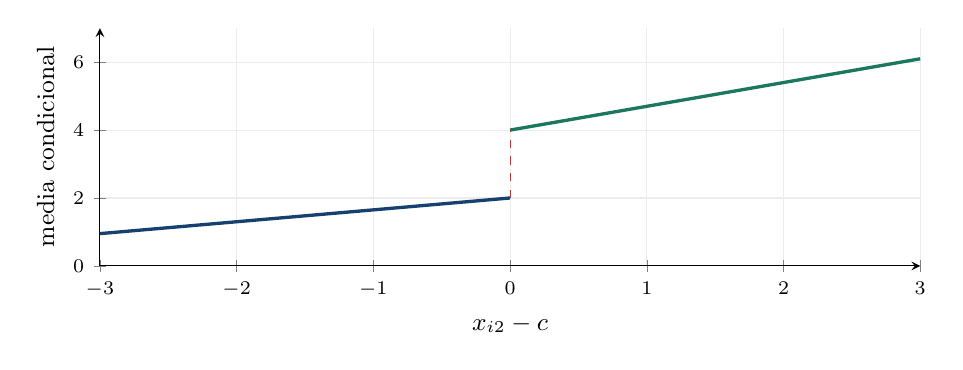
\begin{tikzpicture}\begin{axis}[base,width=12cm,height=4.6cm,xmin=-3,xmax=3,ymin=0,ymax=7,xlabel={$x_{i2}-c$},ylabel={media condicional}]
\addplot[azul,very thick,domain=-3:0]{2+.35*x};
\addplot[verde,very thick,domain=0:3]{4+.7*x};
\addplot[rojo,dashed] coordinates {(0,2)(0,4)};
\end{axis}\end{tikzpicture}
\end{center}
\clearpage\tableofcontents

\clearpage
\addcontentsline{toc}{part}{Fundamentos de probabilidad y álgebra lineal}
\pdfbookmark[0]{Fundamentos de probabilidad y álgebra lineal}{parte1}
\section{Datos observados, resultados latentes y preguntas de identificación}\label{unidad1}
Una observación contiene regresores conocidos y un resultado.
Escribimos \(x_i=(x_{i1},\ldots,x_{ik})\T\); su coordenada
\(x_{ij}\) es el valor del regresor \(j\) en la fila \(i\).
Cuando se usa intercepto, \(x_{i1}=1\).
Antes del muestreo, \(Y_i\) es aleatorio; después de observarlo,
\(y_i\) es un número. Mantener fija la matriz de datos al
calcular una derivada significa que no se deriva \(x_{ij}\).

Un resultado latente \(Y_i^\ast\) puede no coincidir con
el observado. En censura inferior,
\[
Y_i=\begin{cases}0,&Y_i^\ast\le0,\\Y_i^\ast,&Y_i^\ast>0.\end{cases}
\]
El cero indica un conjunto de valores latentes, no un
valor latente conocido exactamente.
En selección, en cambio, \(S_i=0\) puede significar
que no conocemos \(Y_i^\ast\) en absoluto.
Codificar esa ausencia como \(y_i=0\) cambia la información.

La identificación pregunta si distribuciones observables
iguales pueden corresponder a parámetros distintos.
La estimación construye una regla a partir de una muestra.
La optimización encuentra el valor de esa regla.
Son tres preguntas relacionadas, pero distintas:
\[
\text{parámetro}\longmapsto
\text{distribución observable}\longmapsto
\text{muestra}\longmapsto\text{estimador}.
\]
Un máximo numérico no demuestra que el parámetro esté
identificado. Un buen ajuste de medias tampoco demuestra
que el coeficiente tenga una interpretación causal.

\begin{ejemplo}[Ingreso observado]
Si solo se observa ingreso de quienes trabajan,
\(S_i\) señala disponibilidad de ingreso.
Quien no trabaja no necesariamente tiene un salario
potencial de cero. La ecuación salarial y la de
participación son dos relaciones diferentes.
\end{ejemplo}
En discontinuidad se conocerá una regla de elegibilidad,
\(D_i=\mathbf1\{x_{i2}\ge c\}\).
El segundo regresor se mantendrá como \(x_{i2}\)
incluso después de centrarlo: se escribirá \(x_{i2}-c\).
No se lo reemplazará por una letra que esconda el umbral.

Los laboratorios siempre indican cuáles columnas son
datos originales y cuáles operaciones de esos datos
forman un diseño de regresión.
El número de columnas puede cambiar al introducir
interacciones, mientras el número de observaciones
permanece igual. Revisar dimensiones evita
multiplicaciones que parecen razonables pero no existen.

\clearpage
\section{Masa, densidad y distribución mixta: qué se multiplica en una verosimilitud}\label{unidad2}
Una variable discreta asigna probabilidades a puntos;
una variable continua asigna probabilidades a intervalos.
Si \(Y_i^\ast\) tiene densidad \(f\), entonces
\(\Prob(Y_i^\ast=a)=0\), aunque \(f(a)>0\).
Su probabilidad en un intervalo es
\[
\Prob(a<Y_i^\ast<b)=\int_a^b f(t)\dd t.
\]
Una densidad puede superar uno: su integral total,
y no cada altura, debe valer uno.

Para \(Y_i=\max(0,Y_i^\ast)\), aparece una masa puntual:
\[
\Prob(Y_i=0)=\Prob(Y_i^\ast\le0).
\]
Para \(y>0\), su componente continua conserva la densidad
de \(Y_i^\ast\) en ese punto.
La distribución observada es mixta.
La suma de la masa del cero y del área positiva debe ser uno:
\[
\Prob(Y_i^\ast\le0)+\int_0^\infty f(t)\dd t=1.
\]
No se divide la densidad positiva por la probabilidad
de estar por encima de cero, salvo que se esté
condicionando explícitamente en ese evento.

Con independencia entre filas, la verosimilitud del
modelo mixto multiplica masas para los ceros
y densidades para los positivos.
Puede interpretarse como una densidad respecto de
una medida que suma una masa de Dirac en cero
y la medida de longitud sobre los positivos.

\begin{ejemplo}[Normal centrada de escala uno]
Si \(Y_i^\ast\sim\mathcal N(0,1)\), la masa censurada
es \(1/2\), y el área de la densidad para \(y>0\)
también es \(1/2\).
La altura en \(y=1\) es aproximadamente .24197072.
Esta altura no es la probabilidad de observar
exactamente el número uno.
\end{ejemplo}
En una muestra truncada solo llegan registros positivos.
Entonces se observa la densidad condicional
\(f(y)/\Prob(Y_i^\ast>0)\) para \(y>0\),
y no se conservan ceros censurados.
Truncamiento y censura generan objetivos diferentes.

En Heckman, \(S_i\) es discreto y el resultado seleccionado
es continuo. Su contribución es una probabilidad cuando
\(S_i=0\), y una densidad conjunta de resultado y selección
cuando \(S_i=1\).
Esta estructura se deducirá integrando el error de
selección, antes de derivar cualquier coeficiente.

\clearpage
\section{Esperanza condicional: calcular antes de interpretar un coeficiente}\label{unidad3}
La esperanza de una respuesta combina valores posibles
con sus probabilidades. Para una variable discreta,
\[
\E[Y_i\mid x_i]=\sum_y y\,\Prob(Y_i=y\mid x_i).
\]
Para una variable continua con densidad condicional,
\[
\E[Y_i\mid x_i]=\int_{\mathbb R} y f(y\mid x_i)\dd y,
\]
si la integral absoluta es finita.
En una distribución mixta se suman ambas contribuciones.
En Tobit el cero no aporta al primer momento,
pero su probabilidad influye en la masa que queda positiva.

La linealidad se comprueba expandiendo la suma o integral:
\[
\E[aY_i+bV_i\mid x_i]
=a\E[Y_i\mid x_i]+b\E[V_i\mid x_i],
\]
cuando \(a,b\) son constantes dados los condicionantes.
Esta identidad no exige independencia.
La independencia sí importa al factorizar
esperanzas de productos.

Si el modelo latente es
\(Y_i^\ast=\sum_jx_{ij}\beta_j+\varepsilon_i\)
y \(\E[\varepsilon_i\mid x_i]=0\),
\[
\E[Y_i^\ast\mid x_i]=\sum_jx_{ij}\beta_j.
\]
Pero aplicar una función no lineal y después promediar
no equivale a aplicarla a la media:
\[
\E[\max(0,Y_i^\ast)\mid x_i]
\ne\max(0,\E[Y_i^\ast\mid x_i])
\]
en general.
La censura rompe esa sustitución.

\begin{ejemplo}[Dos valores latentes]
Si \(Y_i^\ast=-1\) o \(1\), ambos con probabilidad \(1/2\),
su media es cero.
El observado \(\max(0,Y_i^\ast)\) vale cero o uno;
su media es \(1/2\), no cero.
\end{ejemplo}
En selección, \(\E[\varepsilon_i\mid x_i,z_i,S_i=1]\)
puede ser diferente de cero aunque
\(\E[\varepsilon_i\mid x_i,z_i]=0\).
Condicionar en un evento que depende de otro error
correlacionado cambia la distribución relevante.

En discontinuidad no se interpretará una media
de toda la mitad derecha como la media exactamente
en el umbral. Se tomarán límites de medias condicionales.
La operación de promediar y la de aproximar un límite
deben distinguirse antes de formular el efecto causal.

\clearpage
\section{Varianza: abrir el cuadrado y la ley de varianza total}\label{unidad4}
La varianza mide dispersión alrededor de la media:
\[
\Var(Y_i\mid x_i)
=\E[(Y_i-\E[Y_i\mid x_i])^2\mid x_i].
\]
Al abrir el cuadrado aparecen tres términos.
Los condicionantes hacen fija la media interna:
\[
\Var(Y_i\mid x_i)
=\E[Y_i^2\mid x_i]-\{\E[Y_i\mid x_i]\}^2.
\]
No es el segundo momento por sí solo.
Si una respuesta es siempre diez, su segundo momento
es cien y su varianza es cero.

Para obtener la varianza no condicionada, escribamos
\[
Y_i-\E[Y_i]
=(Y_i-\E[Y_i\mid x_i])
+(\E[Y_i\mid x_i]-\E[Y_i]).
\]
La esperanza del producto cruzado es cero,
porque el primer término tiene media condicional cero.
Por tanto,
\[
\Var(Y_i)
=\E[\Var(Y_i\mid x_i)]
+\Var(\E[Y_i\mid x_i]).
\]
La dispersión total contiene variación dentro de un
valor de los regresores y variación entre sus medias.

En un modelo lineal con error homocedástico,
la primera parte puede ser constante.
En Tobit, incluso con error latente de varianza constante,
la varianza observada depende de los regresores
porque cambia la probabilidad de censura.
En Heckman cambia al condicionar en selección.

\begin{ejemplo}[Mezcla de dos grupos]
Supongamos grupos de igual probabilidad con medias
dos y cuatro, y varianza interna uno en cada grupo.
La media global es tres.
La varianza entre medias es
\(\{(2-3)^2+(4-3)^2\}/2=1\).
La varianza total es \(1+1=2\).
\end{ejemplo}
La incertidumbre de un estimador es una varianza
entre muestras repetidas.
La variación de una nueva respuesta es otra varianza.
Una predicción puede tener pequeño error estándar
aunque las respuestas individuales sean muy dispersas.

Esta diferencia reaparecerá en los intervalos:
estimar una media, un efecto de tratamiento o
una respuesta individual exige decidir primero
qué variable aleatoria se está estudiando.

\clearpage
\section{Covarianza de vectores: desarrollar cada entrada y cada producto cruzado}\label{unidad5}
Para un vector aleatorio \(V=(V_1,\ldots,V_k)\T\)
con segundos momentos finitos, la matriz de covarianza es
\[
\Cov(V)=\E[(V-\E[V])(V-\E[V])\T].
\]
Su entrada \((j,l)\) es
\[
\Cov(V_j,V_l)=\E[V_jV_l]-\E[V_j]\E[V_l].
\]
La diagonal contiene varianzas; las entradas cruzadas
pueden ser negativas.
La matriz es simétrica porque \(V_jV_l=V_lV_j\).

Para \(v\in\mathbb R^k\), abrir la forma cuadrática da
\[
v\T\Cov(V)v
=\sum_{j=1}^k\sum_{l=1}^k v_jv_l\Cov(V_j,V_l)
=\Var\left(\sum_jv_jV_j\right)\ge0.
\]
La no negatividad se refiere a toda la forma,
y no al signo de cada entrada.
Con dos coordenadas,
\[
\Var(V_1+V_2)=\Var(V_1)+\Var(V_2)+2\Cov(V_1,V_2).
\]
Con tres hay tres varianzas y tres covarianzas
multiplicadas por dos.

Si \(M\) es una matriz fija,
\[
\E[MV]=M\E[V],\qquad \Cov(MV)=M\Cov(V)M\T.
\]
La segunda identidad se deduce sustituyendo
\(MV-\E[MV]=M(V-\E[V])\) dentro del producto exterior.
En una regresión, condicionar en el diseño permite
considerar fija la matriz que multiplica las respuestas.

\begin{ejemplo}[Una combinación de dos coeficientes]
Si la covarianza es
\(\begin{psmallmatrix}1&-.3\\-.3&.5\end{psmallmatrix}\),
la varianza de \(\widehat\beta_1+2\widehat\beta_2\)
es \(1+4(.5)+4(-.3)=1.8\).
Omitir el producto cruzado daría tres.
\end{ejemplo}
El estimador de un salto en discontinuidad es una
combinación de coeficientes o de predicciones en dos lados.
La covarianza de esa combinación se calcula mediante
esta operación, manteniendo los términos cruzados.

En Heckman se agregará además la incertidumbre
del regresor generado por la primera etapa.
Las covarianzas entre etapas se estudiarán con
ecuaciones apiladas; no se asumirá que pueden omitirse.

\clearpage
\section{Matrices de datos: filas, transpuesta y seis productos distintos}\label{unidad6}
Para tres regresores, incluyendo intercepto,
\[
X=\begin{pmatrix}
1&x_{12}&x_{13}\\
1&x_{22}&x_{23}\\
\vdots&\vdots&\vdots\\
1&x_{n2}&x_{n3}
\end{pmatrix},\qquad
y=\begin{pmatrix}y_1\\y_2\\\vdots\\y_n\end{pmatrix}.
\]
La matriz \(X\) tiene \(n\) filas y tres columnas.
Su transpuesta tiene tres filas y \(n\) columnas.
Multiplicar fila de la transpuesta por columna del diseño produce
\[
X\T X=
\begin{pmatrix}
n&\sum_i x_{i2}&\sum_i x_{i3}\\
\sum_i x_{i2}&\sum_i x_{i2}^2&\sum_i x_{i2}x_{i3}\\
\sum_i x_{i3}&\sum_i x_{i2}x_{i3}&\sum_i x_{i3}^2
\end{pmatrix}.
\]
La matriz conserva el nombre de la operación y
las sumas se muestran dentro de cada entrada.
Las tres posiciones repetidas por simetría
provienen del mismo producto, en orden inverso.

Para tres filas \((1,-1,0),(1,0,1),(1,2,1)\),
\[
X\T X=
\begin{pmatrix}3&1&2\\1&5&2\\2&2&2\end{pmatrix}.
\]
Por ejemplo, el cruce de pendientes es
\((-1)(0)+(0)(1)+(2)(1)=2\).
La suma de cuadrados del segundo regresor es
\((-1)^2+0^2+2^2=5\).

El producto con respuestas es otra columna:
\[
X\T y=
\begin{pmatrix}
\sum_i y_i\\\sum_i x_{i2}y_i\\\sum_i x_{i3}y_i
\end{pmatrix}.
\]
No tiene dimensión \(n\), sino tres.
Una multiplicación que intenta sumar columnas
de longitudes distintas no representa un modelo válido.

En discontinuidad se construirán columnas de
\(D_i,x_{i2}-c,D_i(x_{i2}-c)\).
En Heckman se agregará una columna con
\(\varphi(\sum_lz_{il}\widehat\gamma_l)/
\Phi(\sum_lz_{il}\widehat\gamma_l)\).
Cada matriz se desplegará con sus datos;
la transformación de columnas no se ocultará
bajo nombres nuevos para las filas.

\clearpage
\section{Producto exterior, rango y existencia de una inversa}\label{unidad7}
Una fila como columna \(x_i\) genera el producto exterior
\[
x_ix_i\T=
\begin{pmatrix}
x_{i1}^2&x_{i1}x_{i2}&\cdots\\
x_{i2}x_{i1}&x_{i2}^2&\cdots\\
\vdots&\vdots&\ddots
\end{pmatrix}.
\]
Su rango es uno si \(x_i\ne0\):
multiplicarlo por cualquier vector produce
\(x_i(x_i\T v)\), un múltiplo de la misma columna.
Sumar productos exteriores puede aumentar el rango:
\[
X\T X=\sum_i x_ix_i\T.
\]
Para cualquier dirección,
\[
v\T X\T Xv
=\sum_i\left(\sum_jx_{ij}v_j\right)^2.
\]
La forma es cero precisamente cuando \(Xv=0\).
Por ello \(X\T X\) es invertible si y solo si
las columnas de \(X\) son linealmente independientes.

Si \(x_{i3}=2x_{i2}\) para toda fila,
\(v=(0,2,-1)\T\) satisface \(Xv=0\).
Los coeficientes pueden cambiar en esa dirección
sin cambiar ningún producto lineal.
No se puede identificar por separado
el efecto de esas dos columnas.

Con pesos no negativos, la forma cuadrática
se convierte en suma de cuadrados ponderados.
Las filas con peso cero no ayudan a recuperar el rango.
En cada aplicación se mostrará la función
de ponderación directamente dentro de la suma.

\begin{ejemplo}[Dos puntos por lado]
Para ajustar una recta con intercepto en un lado
de un umbral, hacen falta al menos dos valores
distintos de \(x_{i2}-c\) con peso positivo.
Dos filas con exactamente el mismo valor
solo repiten la misma dirección.
\end{ejemplo}
Más filas no garantizan más información independiente.
Una matriz casi singular también puede tener inversa,
pero produce mucha incertidumbre y sensibilidad numérica.
La existencia matemática de una inversa debe
distinguirse de la precisión con que se puede calcular.

Si una columna se agrega en una segunda etapa,
debe comprobarse otra vez el rango.
La razón inversa de Mills puede variar muy poco
o aproximarse a una combinación de regresores existentes.
En ese caso la corrección de selección puede
estar identificada débilmente, aunque se pueda
escribir formalmente una matriz ampliada.

\clearpage
\section{Derivar mínimos cuadrados sin recordar una fórmula}\label{unidad8}
El objetivo de mínimos cuadrados es
\[
\sum_{i=1}^n\left(y_i-\sum_{j=1}^kx_{ij}\beta_j\right)^2.
\]
Los datos son constantes al derivar respecto de \(\beta_l\).
La regla de la cadena multiplica la derivada del
cuadrado por la derivada de la discrepancia:
\[
\frac{\partial}{\partial\beta_l}
\sum_i\left(y_i-\sum_jx_{ij}\beta_j\right)^2
=-2\sum_i x_{il}\left(y_i-\sum_jx_{ij}\beta_j\right).
\]
Igualar a cero y abrir la suma interna produce
\[
\sum_i x_{il}y_i
=\sum_{j=1}^k\beta_j\sum_i x_{il}x_{ij},
\qquad l=1,\ldots,k.
\]
Estas son las ecuaciones normales.
Reunir sus coordenadas da \(X\T X\widehat\beta=X\T y\).

La segunda derivada entre dos coeficientes es
\[
\frac{\partial^2}{\partial\beta_l\partial\beta_h}
\sum_i\left(y_i-\sum_jx_{ij}\beta_j\right)^2
=2\sum_i x_{il}x_{ih}.
\]
La Hessiana es \(2X\T X\).
Con rango completo, su forma cuadrática es positiva
para cualquier dirección no nula.
La raíz es entonces el mínimo único:
\[
\widehat\beta=(X\T X)^{-1}X\T y.
\]
La inversa aparece después de deducir el sistema,
no como un objeto que reemplaza a las sumas.

En tres columnas, la primera ecuación dice
\[
\sum_i y_i=n\widehat\beta_1
+\widehat\beta_2\sum_i x_{i2}
+\widehat\beta_3\sum_i x_{i3}.
\]
Las otras dos incorporan cuadrados y cruces.
Un intercepto impone que la suma de residuos sea cero.

\begin{ejemplo}[Una recta exacta]
Con \(x_{i2}=0,1,2\) y \(y_i=1,3,5\),
\[
\begin{pmatrix}3&3\\3&5\end{pmatrix}
\begin{pmatrix}\widehat\beta_1\\\widehat\beta_2\end{pmatrix}
=\begin{pmatrix}9\\13\end{pmatrix}.
\]
Restar las filas produce \(2\widehat\beta_2=4\);
la pendiente es dos y el intercepto uno.
\end{ejemplo}
La fórmula estima la mejor proyección lineal
para cualquier respuesta numérica.
Su interpretación como parámetro verdadero
exige hipótesis sobre la media condicional;
la minimización sola no las establece.

\clearpage
\section{Esperanza exacta de MCO condicionado en el diseño}\label{unidad9}
Supongamos el modelo lineal correcto
\[
Y_i=\sum_jx_{ij}\beta_j+\varepsilon_i,\qquad
\E[\varepsilon_i\mid X]=0,
\]
con \(X\) de rango completo.
Apilar filas produce \(Y=X\beta+\varepsilon\).
Sustituir en el estimador ya deducido da
\[
\begin{aligned}
\widehat\beta
&=(X\T X)^{-1}X\T(X\beta+\varepsilon)\\
&=\beta+(X\T X)^{-1}X\T\varepsilon.
\end{aligned}
\]
La segunda igualdad usa
\((X\T X)^{-1}X\T X=I_k\).
Condicionar en \(X\) permite sacar las matrices
fuera de la esperanza:
\[
\E[\widehat\beta\mid X]
=\beta+(X\T X)^{-1}X\T\E[\varepsilon\mid X]
=\beta.
\]
Este es un resultado exacto finito cuando las
esperanzas existen y el modelo lineal de media es correcto.

Si la media del error no es cero, la expresión cambia:
\[
\E[\widehat\beta\mid X]-\beta
=(X\T X)^{-1}X\T\E[\varepsilon\mid X].
\]
En selección, esa media puede contener la
razón inversa de Mills.
En censura, las respuestas observadas no siguen
la misma media lineal que las latentes.
Aplicar MCO a sus datos no conserva automáticamente
la primera demostración.

\begin{ejemplo}[Regresor omitido]
Si en realidad
\(Y=X\beta+\delta V+\varepsilon\),
con \(V\) una columna omitida conocida dado el diseño,
el sesgo condicionado es
\[
\delta(X\T X)^{-1}X\T V.
\]
No basta que \(V\) tenga media cero:
importa su proyección sobre las columnas incluidas.
\end{ejemplo}
En regresión discontinua, si una recta local fuera
exactamente la media en todo el intervalo usado,
sus coeficientes serían insesgados condicionados.
Si la media tiene curvatura omitida, aparece
un término de aproximación que se convierte
en sesgo de extrapolación al umbral.

La propiedad de insesgamiento no se deduce de que
el algoritmo converja ni de que los residuos
sumen cero. Se deduce de la distribución
de errores y del diseño del modelo.

\clearpage
\section{Covarianza exacta de todos los coeficientes de MCO}\label{unidad10}
La expansión lineal del estimador implica
\[
\Cov(\widehat\beta\mid X)
=(X\T X)^{-1}X\T\Cov(\varepsilon\mid X)X(X\T X)^{-1}.
\]
Se conserva la matriz de errores entre los factores del diseño.
Si las respuestas son independientes dado \(X\)
y \(\Var(\varepsilon_i\mid X)=\sigma_i^2\),
la matriz de errores es diagonal.
Multiplicar sus filas da
\[
\Cov(\widehat\beta\mid X)
=(X\T X)^{-1}
\left[\sum_i\sigma_i^2x_ix_i\T\right](X\T X)^{-1}.
\]
Con homocedasticidad \(\sigma_i^2=\sigma^2\),
la suma central es \(\sigma^2X\T X\), y
\[
\Cov(\widehat\beta\mid X)=\sigma^2(X\T X)^{-1}.
\]
Esta simplificación necesita igualdad de varianzas.
No se aplica por analogía a un resultado seleccionado
con varianza que depende de los regresores.

Cada entrada se puede abrir:
\[
\begin{aligned}
&\Cov(\widehat\beta_j,\widehat\beta_l\mid X)\\
&=\sum_{r=1}^k\sum_{s=1}^k
[(X\T X)^{-1}]_{jr}
\left[\sum_i\sigma_i^2x_{ir}x_{is}\right]
[(X\T X)^{-1}]_{sl}.
\end{aligned}
\]
Cada coordenada usa todas las covarianzas entre columnas.
Para tres coeficientes, la suma tiene nueve productos
de entradas de la inversa y de la matriz central.
La diagonal no se calcula invirtiendo cada diagonal por separado.

\begin{ejemplo}[Diseño de tres puntos]
Para intercepto y \(x_{i2}=0,1,2\),
\[
(X\T X)^{-1}
=\frac16\begin{pmatrix}5&-3\\-3&3\end{pmatrix}.
\]
Con \(\sigma^2=1\), las varianzas son \(5/6\) y \(1/2\),
y la covarianza es \(-1/2\).
La varianza de la predicción en \(x_{i2}=1\) es
\(5/6+1/2-1=1/3\).
\end{ejemplo}
Una covarianza negativa puede reducir la incertidumbre
de una combinación de coeficientes.
Omitirla modifica intervalos de predicciones
y de saltos entre dos ajustes.

La normalidad de los errores no fue necesaria
para esta identidad de covarianza.
Con errores normales, una transformación lineal del
vector de respuestas produce además una distribución
normal exacta de los coeficientes condicionado en \(X\).
Sin normalidad, la identidad de momentos sigue válida
si existen los segundos momentos especificados.

\clearpage
\section{Mínimos cuadrados ponderados: derivadas con el peso visible}\label{unidad11}
Un ajuste local triangular utiliza, para \(h>0\),
\[
\left(1-\frac{|x_{i2}-c|}{h}\right)
\mathbf1\{|x_{i2}-c|\le h\}.
\]
El objetivo conserva esa función dentro de cada sumando:
\[
\sum_i
\left(1-\frac{|x_{i2}-c|}{h}\right)\mathbf1\{|x_{i2}-c|\le h\}
\left(y_i-\sum_jx_{ij}\beta_j\right)^2.
\]
Derivar respecto del coeficiente \(l\) genera
\[
-2\sum_i
\left(1-\frac{|x_{i2}-c|}{h}\right)\mathbf1\{|x_{i2}-c|\le h\}
x_{il}\left(y_i-\sum_jx_{ij}\beta_j\right).
\]
El ancho de banda está fijo al derivar;
el peso no cambia con \(\beta_l\).

Las ecuaciones normales completas son
\[
\begin{aligned}
&\sum_{j=1}^k\beta_j
\sum_i\left(1-\frac{|x_{i2}-c|}{h}\right)
\mathbf1\{|x_{i2}-c|\le h\}x_{il}x_{ij}\\
&=\sum_i\left(1-\frac{|x_{i2}-c|}{h}\right)
\mathbf1\{|x_{i2}-c|\le h\}x_{il}y_i.
\end{aligned}
\]
La matriz de la izquierda se construye
con esos productos fila por fila.
Si es invertible, existe un mínimo único.
La condición de rango se aplica a las filas
con peso estrictamente positivo.

Los pesos del kernel dan mayor influencia a los puntos
cercanos al umbral. No son necesariamente inversas
de varianzas. La covarianza de coeficientes necesita
el cuadrado de los pesos en su matriz central:
\[
\begin{aligned}
&\left[\sum_i K\left(\frac{x_{i2}-c}{h}\right)x_ix_i\T\right]^{-1}\\
&\quad\cdot
\left[\sum_i K\left(\frac{x_{i2}-c}{h}\right)^2\sigma_i^2x_ix_i\T\right]
\left[\sum_i K\left(\frac{x_{i2}-c}{h}\right)x_ix_i\T\right]^{-1}.
\end{aligned}
\]
Aquí \(K(u)=(1-|u|)\mathbf1\{|u|\le1\}\)
es una función especificada; en los laboratorios
se sustituye por su expresión completa.

Si todos los errores tienen varianza uno,
el factor central no coincide en general
con la primera suma, porque los pesos al cuadrado
no son iguales a los pesos.
Por eso invertir la primera matriz por sí sola
no calcula la dispersión exacta de ese ajuste local.
La homocedasticidad de errores y la elección
de pesos son dos decisiones diferentes.

\clearpage
\section{Taylor multivariable: conservar el resto y el segmento}\label{unidad12}
Para una función diferenciable y un cambio
\(\Delta\in\mathbb R^k\), recorramos
\(\beta+t\Delta\), con \(0\le t\le1\).
Integrar la regla de la cadena da la identidad
\[
f(\beta+\Delta)-f(\beta)
=\int_0^1\nabla f(\beta+t\Delta)\T\Delta\dd t.
\]
Con segundas derivadas continuas,
\[
\begin{aligned}
f(\beta+\Delta)
={}&f(\beta)+\nabla f(\beta)\T\Delta\\
&+\int_0^1(1-t)\Delta\T\nabla^2f(\beta+t\Delta)\Delta\dd t.
\end{aligned}
\]
El segundo orden en el punto inicial aproxima la integral.
No es una igualdad global salvo que la Hessiana
permanezca constante a lo largo del segmento.

Para el gradiente, la identidad exacta es
\[
\nabla f(\beta+\Delta)
=\nabla f(\beta)
+\left[\int_0^1\nabla^2f(\beta+t\Delta)\dd t\right]\Delta.
\]
No se presupone un mismo punto intermedio para
todas las coordenadas. El valor medio escalar
no se convierte automáticamente en una identidad
vectorial con una sola Hessiana intermedia.

Newton aproxima la integral por la Hessiana inicial
y pide gradiente aproximado cero:
\[
\nabla^2f(\beta)\Delta=-\nabla f(\beta).
\]
Resolver un sistema mantiene la interacción
entre coordenadas. Dividir cada componente del
gradiente por su entrada diagonal omite
las derivadas cruzadas.

\begin{ejemplo}[Un cruce visible]
Para \(f(\beta_1,\beta_2)=\beta_1^2+\beta_1\beta_2+\beta_2^2\),
la Hessiana es
\(\begin{psmallmatrix}2&1\\1&2\end{psmallmatrix}\).
El término cuadrático es
\(\Delta_1^2+\Delta_1\Delta_2+\Delta_2^2\).
\end{ejemplo}
En Tobit se derivará conjuntamente coeficientes y escala.
En Heckman aparecerá además la correlación de errores.
La amplitud del paso se controlará reevaluando
la verosimilitud original, porque una aproximación
local no asegura mejora con paso completo.

El mismo Taylor explica el sesgo de un polinomio local
en discontinuidad: los términos de curvatura
omitidos no desaparecen por haber ajustado
una recta con muchos decimales.

\clearpage
\section{Método delta: propagar covarianza a funciones no lineales}\label{unidad13}
Supongamos
\(\sqrt n(\widehat\theta-\theta_\star)
\Rightarrow\mathcal N(0,V)\).
Para una función diferenciable \(g\), Taylor local da
\[
g(\widehat\theta)-g(\theta_\star)
=\nabla g(\theta_\star)\T(\widehat\theta-\theta_\star)
+o_p(n^{-1/2}),
\]
con las condiciones correspondientes de regularidad.
Multiplicar por \(\sqrt n\) produce
\[
\sqrt n[g(\widehat\theta)-g(\theta_\star)]
\Rightarrow\mathcal N
\left(0,\nabla g(\theta_\star)\T V\nabla g(\theta_\star)\right).
\]
Para varias funciones se usa el Jacobiano y su transpuesta.

El cociente \(g(u,v)=u/v\), con \(v\ne0\), tiene derivada
\[
\left(\frac1v,-\frac u{v^2}\right)\T.
\]
La propagación completa es
\[
\frac{\Var(\widehat u)}{v^2}
+\frac{u^2}{v^4}\Var(\widehat v)
-\frac{2u}{v^3}\Cov(\widehat u,\widehat v).
\]
El cruce importa porque los dos saltos de una
discontinuidad fuzzy usan las mismas observaciones.
Su independencia no se deduce de que uno
se refiera a resultados y el otro a tratamiento.

En Tobit, la media observada depende de
\(\beta_1,\ldots,\beta_k,\sigma\).
Su error estándar incluye covarianzas de
coeficientes con la escala.
En Heckman, Mills depende de todos los
parámetros de selección.

\begin{ejemplo}[Una razón]
Con \(u=2,v=.5\), varianzas .04 y .01,
y covarianza .01, la varianza aproximada es
\[
.04/.25+4(.01)/.0625-4(.01)/.125=.48.
\]
Eliminar la covarianza daría .80.
\end{ejemplo}
El método es una aproximación local.
Si el denominador se acerca a cero,
las derivadas crecen sin límite y la
aproximación normal regular puede ser deficiente.
Una primera etapa débil no se resuelve
imprimiendo un intervalo de Wald rutinario.

Las funciones \(u,v\) de este ejemplo son
cantidades estimadas, no cambios de nombre
de los datos de una fila.
En las aplicaciones se escribirá el numerador
y denominador como saltos, sumas o funciones
completas de los parámetros.

\clearpage
\section{Verosimilitud, score e información: demostrar la igualdad de momentos}\label{unidad14}
La verosimilitud fija los datos y evalúa
su masa o densidad bajo distintos parámetros.
El score es el vector de derivadas del logaritmo,
\(\nabla_\theta\ell(\theta;y)\).
La información observada es el negativo de su Hessiana.
La esperada promedia esa curvatura bajo el modelo.

Bajo regularidad, derivar la integral uno da
\[
\begin{aligned}
0&=\frac{\partial}{\partial\theta_j}\int f_\theta(y)\dd y\\
&=\int
\frac{\partial\log f_\theta(y)}{\partial\theta_j}
f_\theta(y)\dd y.
\end{aligned}
\]
Es la esperanza cero del score.
Se requiere intercambio válido de derivación e integración.
Para una distribución mixta se incluyen la masa
y la parte continua con su medida de referencia fija.

Derivar una segunda vez genera dos términos:
la segunda derivada del logaritmo y el
producto de sus primeras derivadas.
Su suma esperada es cero:
\[
-\E[\nabla_\theta^2\ell(\theta;Y)]
=\E[\nabla_\theta\ell(\theta;Y)
\nabla_\theta\ell(\theta;Y)\T].
\]
La derecha es la covarianza del score
porque su esperanza se anula.
En un modelo incorrecto, estas dos matrices
pueden ser distintas y aparece un sándwich.

La identidad no demuestra que el estimador
no lineal tenga covarianza exacta igual
a la inversa de la información.
Taylor de sus ecuaciones y un límite central
justifican esa aproximación en muestras grandes,
con identificación y un máximo interior regular.

\begin{ejemplo}[Escala]
Dividir la log-verosimilitud por \(n\)
divide la curvatura por \(n\).
Su inversa se multiplica por \(n\).
La covarianza de \(\widehat\theta\)
y la de \(\sqrt n(\widehat\theta-\theta_\star)\)
requieren escalas distintas.
\end{ejemplo}
En Tobit la Hessiana observada depende de
qué filas están censuradas.
En Heckman depende de selección y resultados.
En probit, incluso manteniendo el diseño fijo,
la curvatura observada cambia con las respuestas.

Se comprobará esperanza cero del score
por integración explícita en Tobit,
además de esta demostración general.
Esa verificación separa la teoría del
redondeo numérico de un ajuste concreto.

\clearpage
\section{Momentos exactos y límites asintóticos: distinguir sus condiciones}\label{unidad15}
Una afirmación exacta describe una muestra de tamaño fijo.
Una asintótica describe una secuencia cuando crece \(n\).
En MCO de media correctamente especificada,
la esperanza exacta se calculó por linealidad.
En modelos no lineales, el estimador puede
no existir en algunas realizaciones.

La convergencia
\[
\sqrt n(\widehat\theta-\theta_\star)
\Rightarrow\mathcal N(0,V)
\]
no demuestra por sí sola convergencia de
esperanzas y varianzas.
Una pequeña probabilidad de valores enormes
puede afectar mucho los momentos.
Se necesita control adicional de colas.

En un modelo censurado, todas las respuestas cero
pueden tener probabilidad positiva.
Disminuir indefinidamente el intercepto hace
que la probabilidad de ese evento se acerque a uno,
sin alcanzar un máximo finito.
En probit, todas las selecciones uno
producen un problema análogo.

Restringir coeficientes a un conjunto compacto,
escala lejos de cero y correlación lejos
de sus extremos garantiza una región controlada.
Si el objetivo es continuo, alcanza un máximo.
Un criterio de desempate define una regla finita.
Sus momentos son los de ese procedimiento
restringido, no los del máximo sin restricciones.

\begin{ejemplo}[Curvatura frente a promedio]
La inversa de una Hessiana en una muestra
describe curvatura local.
Para obtener \(\E[\widehat\beta_j]\),
hay que promediar la regla de estimación
sobre todas las muestras de su distribución.
No se toma la inversa de un único ajuste.
\end{ejemplo}
Los laboratorios lineales de discontinuidad
permiten momentos exactos condicionados.
Para Tobit y Heckman se estudiarán
límites, aproximaciones locales y sumas
o integrales sobre patrones observables.

Los decimales impresos son aproximaciones
cuando dependen de raíces de ecuaciones.
Se distinguirá \(\approx\) de una identidad.
La precisión de un cálculo de ocho dígitos
no elimina la incertidumbre muestral
ni garantiza existencia del estimador.

\clearpage
\section{Variables instrumentales: construir cada ecuación de momentos}\label{unidad16}
Si
\(Y_i=\sum_jx_{ij}\beta_j+\varepsilon_i\)
y hay regresores correlacionados con el error,
un instrumento \(z_{il}\) exige
\(\E[z_{il}\varepsilon_i]=0\).
Sustituir el modelo produce
\[
\E\left[z_{il}\left(Y_i-\sum_jx_{ij}\beta_j\right)\right]=0.
\]
La versión muestral es
\[
\sum_i z_{il}y_i
=\sum_j\beta_j\sum_i z_{il}x_{ij},
\qquad l=1,\ldots,q.
\]
Con tantos instrumentos como coeficientes,
el sistema es cuadrado. Su identificación
necesita rango completo de los productos
instrumento por regresor en población.

Con instrumentos adicionales, la proyección
sobre sus columnas conduce a
\[
\widehat\beta_{\mathrm{IV}}
=\left[X\T Z(Z\T Z)^{-1}Z\T X\right]^{-1}
X\T Z(Z\T Z)^{-1}Z\T y.
\]
La entrada \((l,j)\) de \(Z\T X\) es
\(\sum_i z_{il}x_{ij}\).
La entrada \((l,h)\) de \(Z\T Z\) es
\(\sum_i z_{il}z_{ih}\).
Estos productos se mantienen visibles;
no se reemplazan por letras auxiliares.

\begin{ejemplo}[Un instrumento y un regresor]
Sin intercepto, con \(z=(1,2,3)\T\),
\(x=(1,1,2)\T\), \(y=(2,3,5)\T\), se resuelve
\[
(1)(2)+(2)(3)+(3)(5)
=\beta[(1)(1)+(2)(1)+(3)(2)].
\]
La solución es \(23/9\).
El número no demuestra que el instrumento
sea exógeno: eso es una hipótesis del modelo.
\end{ejemplo}
La discontinuidad fuzzy utiliza elegibilidad
como fuente instrumental del cambio de tratamiento.
La razón entre saltos se interpretará
sobre una población local de cumplidores.

La relevancia necesita un cambio no nulo
en tratamiento. La exclusión exige que la
elegibilidad no cambie directamente el resultado
por una vía adicional no modelada.
Una matriz casi singular refleja debilidad
de información y puede invalidar una
aproximación normal rutinaria para la razón.

\clearpage
\section{Regresores generados: la incertidumbre heredada de una primera etapa}\label{unidad17}
En Heckman, una columna se calcula con parámetros
estimados en un probit:
\[
\frac{\varphi(\sum_l z_{il}\widehat\gamma_l)}
{\Phi(\sum_l z_{il}\widehat\gamma_l)}.
\]
Antes de observar la muestra, esa columna es aleatoria.
Tratarla como conocida omite potencialmente
una parte de la dispersión de segunda etapa.

Una expansión simultánea de sus ecuaciones
incluye dos cambios:
\[
\begin{aligned}
0\approx&
\text{momento en los parámetros verdaderos}\\
&+\frac{\partial\,\text{momento}}{\partial\beta\T}
(\widehat\beta-\beta_\star)
+\frac{\partial\,\text{momento}}{\partial\gamma\T}
(\widehat\gamma-\gamma_\star).
\end{aligned}
\]
Resolver para el primer cambio deja
una parte de su propio error de muestreo
y otra procedente de la primera etapa.
Su covarianza debe propagarlas conjuntamente.

Los dos estimadores comparten observaciones.
No se presume que sean independientes.
Una covarianza poblacional concreta puede
anularse por media condicional cero,
pero esa anulación necesita una demostración.

\begin{ejemplo}[Cambio de una coordenada]
Al mover \(\gamma_l\),
\(\sum_h z_{ih}\gamma_h\) cambia en \(z_{il}\)
por el incremento.
La derivada escalar de Mills multiplica
esa coordenada del dato.
Su tamaño indica cómo afecta la primera etapa
a la nueva columna de una fila.
\end{ejemplo}
Apilar todas las ecuaciones produce un
Jacobiano por bloques. Los bloques cruzados
registran el efecto de \(\gamma\) sobre
los momentos de resultados.
Invertirlo y propagar la covarianza de
los momentos incorpora la incertidumbre.

La corrección no consiste simplemente en
multiplicar todos los errores estándar
por una constante.
Puede modificar cada varianza y cada
covarianza cruzada de manera diferente.

Se desarrollará la matriz con sumas
sobre seleccionados y sobre toda la muestra.
La comparación con \(\gamma\) conocido
mostrará exactamente qué términos
se perderían al ignorar el regresor generado.

\clearpage
\section{Efectos fijos: eliminar interceptos de grupo con sumas explícitas}\label{unidad18}
En un panel,
\[
Y_{it}=\alpha_i+\sum_{j=1}^k x_{itj}\beta_j+\varepsilon_{it}.
\]
El intercepto \(\alpha_i\) es constante dentro del individuo.
Sumar \(T\) ecuaciones y dividir por \(T\) da
\[
\frac1T\sum_sY_{is}
=\alpha_i+\sum_j\left(\frac1T\sum_sx_{isj}\right)\beta_j
+\frac1T\sum_s\varepsilon_{is}.
\]
Restar de la ecuación en el tiempo \(t\) elimina
exactamente ese intercepto:
\[
\begin{aligned}
Y_{it}-\frac1T\sum_sY_{is}
={}&\sum_j\left(x_{itj}-\frac1T\sum_sx_{isj}\right)\beta_j\\
&+\varepsilon_{it}-\frac1T\sum_s\varepsilon_{is}.
\end{aligned}
\]
Las medias se conservan como sumas;
no se renombra cada dato transformado.

Las ecuaciones normales tienen entrada
\[
\sum_i\sum_t
\left(x_{itj}-\frac1T\sum_sx_{isj}\right)
\left(x_{itl}-\frac1T\sum_sx_{isl}\right).
\]
Su lado derecho reemplaza el segundo factor
por \(Y_{it}-T^{-1}\sum_sY_{is}\).
La matriz de productos cruzados usa
exclusivamente variación dentro de individuos.

Una variable constante en el individuo
se convierte en cero.
Su coeficiente no se identifica por
esta transformación. Para interpretar los
otros coeficientes se necesitan condiciones
sobre la relación de los errores con
los regresores del panel completo.

\begin{ejemplo}[Dos tiempos]
Con \(x_{i12}=1,x_{i22}=3\),
la media es dos y los valores centrados
son \(-1,1\).
El intercepto de grupo desaparece,
pero la variación temporal permanece.
\end{ejemplo}
En Tobit, restar medias del observado
\(\max(0,Y_{it}^\ast)\) no elimina
linealmente \(\alpha_i\).
La transformación y la censura no conmutan.
En selección, el error condicionado
también incorpora una media que cambia
con los regresores de selección.

Los efectos fijos y Heckman resuelven
problemas distintos. Agregar dummies
no garantiza que desaparezca la selección
ni que la distribución de los errores
observados sea homocedástica.

\clearpage
\addcontentsline{toc}{part}{Regresión discontinua: identificación y cálculo local}
\pdfbookmark[0]{Regresión discontinua: identificación y cálculo local}{parte19}
\section{Resultados potenciales y elegibilidad en un umbral}\label{unidad19}
Cada individuo tiene dos resultados potenciales:
\(Y_i(0)\) sin tratamiento y \(Y_i(1)\) con tratamiento.
La respuesta observada es
\[
Y_i=(1-T_i)Y_i(0)+T_iY_i(1),\qquad T_i\in\{0,1\}.
\]
No observamos ambos resultados del mismo individuo.
El efecto individual es \(Y_i(1)-Y_i(0)\);
una comparación de dos personas puede incluir
diferencias previas además del tratamiento.

Una regla de elegibilidad fija un umbral conocido \(c\):
\[
D_i=\mathbf1\{x_{i2}\ge c\}.
\]
En un diseño sharp, el tratamiento recibido coincide
con esa regla: \(T_i=D_i\).
Justo por debajo todos son controles;
justo por encima todos son tratados.
El valor \(x_{i2}\) se conserva como dato original.

La asignación cambia abruptamente, pero se requiere
que las medias de los resultados potenciales
sean continuas en el umbral:
\[
x\longmapsto\E[Y_i(0)\mid x_{i2}=x],
\qquad
x\longmapsto\E[Y_i(1)\mid x_{i2}=x].
\]
Estas funciones pueden tener pendientes o curvaturas;
la continuidad no obliga a que sean constantes.

El parámetro local de interés es
\[
\E[Y_i(1)-Y_i(0)\mid x_{i2}=c].
\]
Para una variable de asignación continua,
condicionar en un punto de probabilidad cero
se interpreta mediante una versión continua
de la esperanza condicional.
Su valor se identifica por los límites laterales.

\begin{ejemplo}[Beca y puntaje]
Una beca se concede desde cierto puntaje.
Si las otras determinantes del resultado académico
cambian suavemente alrededor de ese puntaje,
un salto del resultado puede atribuirse al
cambio de elegibilidad bajo esos supuestos.
No se atribuye automáticamente todo contraste
entre puntajes altos y bajos a la beca.
\end{ejemplo}
La hipótesis debe referirse a resultados potenciales,
no a la media observada, que precisamente
puede saltar por el tratamiento.
Una discontinuidad simultánea en otra política
puede invalidar la interpretación de un
único efecto de tratamiento.

\clearpage
\section{Deducir la identificación sharp por límites laterales}\label{unidad20}
Si \(x<c\), la regla implica \(T_i=0\).
Entonces la identidad de respuesta observada da
\[
\E[Y_i\mid x_{i2}=x]=\E[Y_i(0)\mid x_{i2}=x].
\]
Para \(x\ge c\), ocurre lo contrario:
\[
\E[Y_i\mid x_{i2}=x]=\E[Y_i(1)\mid x_{i2}=x].
\]
Al aproximar el umbral por cada lado,
la continuidad de las medias potenciales produce
\[
\begin{aligned}
\lim_{x\downarrow c}\E[Y_i\mid x_{i2}=x]
&=\E[Y_i(1)\mid x_{i2}=c],\\
\lim_{x\uparrow c}\E[Y_i\mid x_{i2}=x]
&=\E[Y_i(0)\mid x_{i2}=c].
\end{aligned}
\]
Restar las dos igualdades y usar linealidad
de esperanza demuestra
\[
\boxed{\lim_{x\downarrow c}\E[Y_i\mid x_{i2}=x]
-\lim_{x\uparrow c}\E[Y_i\mid x_{i2}=x]
=\E[Y_i(1)-Y_i(0)\mid x_{i2}=c]}.
\]
El límite derecho se toma con valores superiores
que descienden hacia \(c\); el izquierdo
con valores inferiores que ascienden.

La diferencia entre promedios de toda una banda
no aparece en esta identidad.
Una banda finita mezcla puntos a distintas
distancias del umbral.
Su interpretación necesita aproximar
las dos funciones hasta el punto de corte.

\begin{ejemplo}[Dos rectas]
Si la media izquierda es \(2+.5(x-c)\)
y la derecha \(5+(x-c)\), los límites son dos y cinco.
El efecto identificado es tres.
Las pendientes son distintas, pero ninguna
altera ese salto en el propio umbral.
\end{ejemplo}
Cambiar el umbral de medición desplaza los
interceptos de una representación lineal,
pero el contraste debe seguir evaluándose
en el umbral que determina la regla.
No se elige un punto por presentar
el mayor salto en los datos.

La identificación es local.
El efecto en una persona muy alejada del corte
no se identifica por esta misma resta.
Transportarlo exige hipótesis adicionales
sobre heterogeneidad de efectos y poblaciones.

\begin{figure}[H]\centering
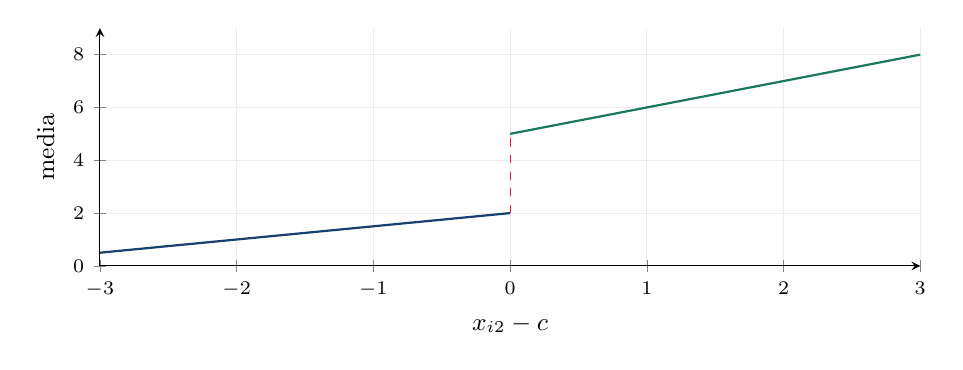
\begin{tikzpicture}\begin{axis}[base,width=12cm,height=4.6cm,xmin=-3,xmax=3,ymin=0,ymax=9,xlabel={$x_{i2}-c$},ylabel={media}]
\addplot[azul,thick,domain=-3:0]{2+.5*x};\addplot[verde,thick,domain=0:3]{5+x};\addplot[rojo,dashed] coordinates {(0,2)(0,5)};
\end{axis}\end{tikzpicture}
\caption{Dos medias laterales; el salto se mide en \(x_{i2}-c=0\).}
\end{figure}

\clearpage
\section{Continuidad no significa independencia en una banda finita}\label{unidad21}
La identificación sharp utiliza continuidad en el umbral.
No afirma que \(D_i\) sea independiente de los
regresores o de los resultados potenciales
en todo intervalo alrededor del corte.
De hecho, \(D_i\) es una función determinista
del dato \(x_{i2}\).

Supongamos que la media de control es
\(2+x_{i2}-c\), y que el tratamiento añade tres.
Con puntajes uniformes dentro de \([c-h,c+h]\),
la media del puntaje a la izquierda es \(c-h/2\);
a la derecha es \(c+h/2\).
Los promedios observados son
\[
2-h/2,\qquad 5+h/2.
\]
Su diferencia es
\[
3+h.
\]
Aunque las medias potenciales son continuas,
la comparación de toda la banda contiene
un término de pendiente.
Ese término desaparece al llevar \(h\) a cero,
pero no en una banda fijada arbitrariamente.

Ajustar rectas laterales permite extrapolar
sus interceptos al punto de corte.
Si esas rectas son correctas, elimina
exactamente el término de pendiente.
Si hay curvatura, quedará un error de
aproximación que se estudiará con Taylor.

Un enfoque de aleatorización local hace
una hipótesis diferente: dentro de una
ventana concreta, la asignación puede
tratarse como un mecanismo aleatorio
con ciertas propiedades.
Eso permite inferencia por asignaciones.
No se deduce simplemente de la continuidad.

\begin{ejemplo}[Dos preguntas]
La continuidad pregunta qué pasa al aproximar
un punto cada vez más de cerca.
La aleatorización local pregunta qué mecanismo
podría generar las asignaciones dentro
de una ventana de tamaño determinado.
\end{ejemplo}
Los diagnósticos de covariables y densidad
aportan evidencia sobre validez,
pero no prueban por sí solos todas
las hipótesis causales no observables.

La proximidad en \(x_{i2}\) reduce ciertas
diferencias sistemáticas si son suaves.
No garantiza que todas las características
sean literalmente idénticas o que
las personas hayan sido sorteadas.

\clearpage
\section{Rectas laterales como una regresión con interacciones}\label{unidad22}
Una representación con pendientes distintas es
\[
Y_i=\beta_1+\beta_2D_i+\beta_3(x_{i2}-c)
+\beta_4D_i(x_{i2}-c)+\varepsilon_i.
\]
Para \(D_i=0\), sustituir produce
\[
\E[Y_i\mid x_{i2}]=\beta_1+\beta_3(x_{i2}-c).
\]
Para \(D_i=1\), se obtiene
\[
\E[Y_i\mid x_{i2}]
=(\beta_1+\beta_2)+(\beta_3+\beta_4)(x_{i2}-c).
\]
El intercepto izquierdo es \(\beta_1\);
el derecho es \(\beta_1+\beta_2\).
La pendiente izquierda es \(\beta_3\);
la derecha es \(\beta_3+\beta_4\).
El salto en el corte es exactamente \(\beta_2\).

La interacción no es una quinta variable
independiente de sus componentes:
se calcula multiplicando \(D_i\)
por el dato centrado \(x_{i2}-c\).
Cada fila del diseño tiene cuatro columnas:
\[
(1,D_i,x_{i2}-c,D_i(x_{i2}-c)).
\]
En el corte, los dos términos de pendiente
valen cero; por eso no confunden el
coeficiente del salto.

Si se usa \(x_{i2}\) sin centrar, el contraste
en el corte contiene también \(\beta_4c\).
En esa parametrización, el coeficiente de
\(D_i\) representa un contraste en cero,
que puede no ser el corte de asignación.
Centrar facilita la interpretación,
sin cambiar las funciones ajustables.

\begin{ejemplo}[Umbral distinto de cero]
Si \(c=50\), los datos 49 y 51
entran como \(-1\) y \(1\).
El salto se evalúa en dato centrado cero,
equivalente al puntaje original 50.
\end{ejemplo}
Imponer \(\beta_4=0\) fuerza pendientes iguales.
Es una restricción del modelo,
no una consecuencia del diseño causal.
Puede alterar el salto estimado si
las funciones laterales son distintas.

Se ajustará esta representación en una
vecindad del corte. Una recta global
usa puntos lejanos y puede depender
fuertemente de una restricción funcional
que la continuidad no impone.

\clearpage
\section{Demostrar equivalencia entre dos rectas y cuatro coeficientes}\label{unidad23}
Considérese ajustar por separado una recta
a cada lado del corte.
Sus parámetros son intercepto y pendiente
izquierdos, e intercepto y pendiente derechos.
La transformación a cuatro coeficientes es
\[
\begin{pmatrix}
\beta_1\\\beta_2\\\beta_3\\\beta_4
\end{pmatrix}
=
\begin{pmatrix}
\text{intercepto izquierdo}\\
\text{intercepto derecho}-\text{intercepto izquierdo}\\
\text{pendiente izquierda}\\
\text{pendiente derecha}-\text{pendiente izquierda}
\end{pmatrix}.
\]
La transformación es invertible:
a partir de \(\beta\) se reconstruyen
los parámetros de ambos lados por sumas.

El objetivo conjunto con pesos de fila es
\[
\begin{aligned}
&\sum_{x_{i2}<c}K\left(\frac{x_{i2}-c}{h}\right)
[y_i-\beta_1-\beta_3(x_{i2}-c)]^2\\
&+\sum_{x_{i2}\ge c}K\left(\frac{x_{i2}-c}{h}\right)
[y_i-(\beta_1+\beta_2)-(\beta_3+\beta_4)(x_{i2}-c)]^2.
\end{aligned}
\]
En los parámetros laterales, el primer sumando
depende solo de la recta izquierda,
y el segundo solo de la derecha.
Por eso se minimizan independientemente.
La transformación invertible lleva esos
mínimos al mínimo de cuatro coeficientes.

La equivalencia exige usar los mismos pesos,
las mismas observaciones y las mismas
restricciones en ambos procedimientos.
Cambiar una pendiente, un ancho de banda
o una muestra rompe esa igualdad.

\begin{ejemplo}[Interpretación de diferencias]
Si las rectas estimadas tienen interceptos
2.1 y 4.8, el salto es \(4.8-2.1=2.7\).
Si sus pendientes son .4 y .9,
la interacción de pendiente es .5.
No se confunde esa diferencia .5
con el salto del intercepto.
\end{ejemplo}
Si las respuestas de los dos lados son
independientes condicionado en el diseño,
sus coeficientes laterales tienen covarianza cero.
La varianza del salto es entonces
la suma de varianzas de los interceptos.
Con dependencia entre lados o grupos,
se debe conservar el cruce.

La regresión conjunta hace aparecer
covarianzas entre \(\beta_1\) y \(\beta_2\),
porque este último resta el primero.
Una parametrización distinta puede tener
covarianzas distintas y aun así dar
el mismo salto y su misma incertidumbre.

\clearpage
\section{Kernel triangular: integrar su área y justificar el peso local}\label{unidad24}
El kernel triangular es
\[
K(u)=(1-|u|)\mathbf1\{|u|\le1\}.
\]
Está entre cero y uno.
Fuera de su soporte, la observación no aporta;
en el centro su peso es uno.
El argumento usado en cada fila es
\((x_{i2}-c)/h\), no un nuevo dato.

Su área total se calcula por simetría:
\[
\int_{-1}^1(1-|u|)\dd u
=2\int_0^1(1-u)\dd u
=2[u-u^2/2]_0^1=1.
\]
El área en cada lado es \(1/2\).
Los momentos en el lado derecho son
\[
\int_0^1u^j(1-u)\dd u
=\frac1{j+1}-\frac1{j+2}
=\frac1{(j+1)(j+2)}.
\]
Para \(j=0,1,2,3,4\) se obtienen
\[
\frac12,\quad\frac16,\quad\frac1{12},
\quad\frac1{20},\quad\frac1{30}.
\]
En el lado izquierdo, los momentos impares
cambian de signo y los pares permanecen iguales.

Multiplicar todos los pesos por una constante
positiva no cambia el mínimo de cuadrados.
Esa constante aparece a ambos lados
de las ecuaciones normales y se cancela.
También se cancela al propagar la covarianza,
si se conserva el cuadrado de los pesos.

\begin{ejemplo}[Ancho de banda dos]
Con \(x_{i2}-c=0,.5,1,1.5,2\),
los pesos son \(1,.75,.5,.25,0\).
El último punto tiene peso cero
aunque esté en la frontera del intervalo.
\end{ejemplo}
La elección del kernel afecta las constantes
de sesgo y varianza.
El ancho de banda controla cuáles puntos
intervienen y cuánto pesan.
No son el mismo objeto.

En los cálculos teóricos se integrará
sobre el argumento escalar \(u\).
Al volver a las observaciones siempre se
reemplazará por su cociente completo
\((x_{i2}-c)/h\).

\begin{figure}[H]\centering
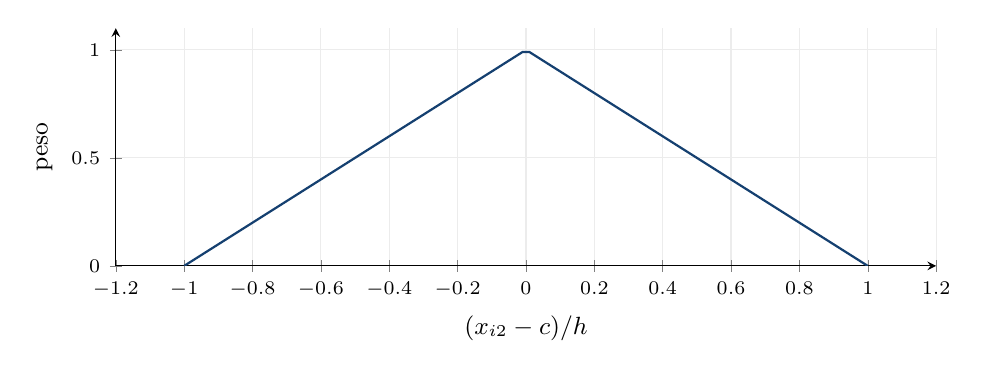
\begin{tikzpicture}\begin{axis}[base,width=12cm,height=4.6cm,xmin=-1.2,xmax=1.2,ymin=0,ymax=1.1,xlabel={$(x_{i2}-c)/h$},ylabel={peso}]
\addplot[azul,thick,domain=-1:1]{1-abs(x)};
\end{axis}\end{tikzpicture}
\caption{Kernel triangular: peso de una observación según distancia normalizada al umbral.}
\end{figure}

\clearpage
\section{Cuatro ecuaciones normales locales con todos los productos visibles}\label{unidad25}
La predicción local es
\[
\beta_1+\beta_2D_i+\beta_3(x_{i2}-c)
+\beta_4D_i(x_{i2}-c).
\]
Su vector de derivadas respecto de los coeficientes es
\((1,D_i,x_{i2}-c,D_i(x_{i2}-c))\T\).
Cada ecuación normal multiplica la discrepancia
por una de esas cuatro entradas y por el peso triangular.

Al reunir las cuatro ecuaciones, la matriz izquierda es
\[
\begin{aligned}
\sum_i&\left(1-\frac{|x_{i2}-c|}{h}\right)
\mathbf1\{|x_{i2}-c|\le h\}\\
&\cdot
\begin{pmatrix}
1&D_i&x_{i2}-c&D_i(x_{i2}-c)\\
D_i&D_i&D_i(x_{i2}-c)&D_i(x_{i2}-c)\\
x_{i2}-c&D_i(x_{i2}-c)&(x_{i2}-c)^2&D_i(x_{i2}-c)^2\\
D_i(x_{i2}-c)&D_i(x_{i2}-c)&D_i(x_{i2}-c)^2&D_i(x_{i2}-c)^2
\end{pmatrix}.
\end{aligned}
\]
Se usó \(D_i^2=D_i\), porque es cero o uno.
El lado derecho es
\[
\sum_i\left(1-\frac{|x_{i2}-c|}{h}\right)
\mathbf1\{|x_{i2}-c|\le h\}
\begin{pmatrix}
y_i\\D_iy_i\\(x_{i2}-c)y_i\\D_i(x_{i2}-c)y_i
\end{pmatrix}.
\]
Cada entrada representa una suma de productos
observables. La esquina \((1,1)\) suma pesos,
no necesariamente el tamaño de muestra total.

Las filas del lado izquierdo tienen
\(D_i=0\); varias entradas quedan cero.
Las del derecho tienen \(D_i=1\).
Los productos de pendiente mantienen
el signo del dato centrado.

El rango exige suficientes valores distintos
con peso positivo en los dos lados.
Si toda la banda tiene \(D_i=1\),
las columnas uno y \(D_i\) son iguales,
y tampoco se distinguen las pendientes.
No se puede estimar un salto con un solo lado.

Esta matriz tiene todas las interacciones
que después se reflejan en su inversa.
Reducirla a cuatro sumas diagonales
eliminaría la geometría del problema.

\clearpage
\section{Intercepto derecho: resolver las dos ecuaciones por eliminación}\label{unidad26}
En el lado derecho se ajusta una recta
con intercepto y pendiente propios.
Su matriz de productos cruzados es
\[
\begin{pmatrix}
\sum_{c\le x_{i2}\le c+h}K(\frac{x_{i2}-c}{h})
&
\sum_{c\le x_{i2}\le c+h}K(\frac{x_{i2}-c}{h})(x_{i2}-c)\\
\sum_{c\le x_{i2}\le c+h}K(\frac{x_{i2}-c}{h})(x_{i2}-c)
&
\sum_{c\le x_{i2}\le c+h}K(\frac{x_{i2}-c}{h})(x_{i2}-c)^2
\end{pmatrix}.
\]
Multiplica el vector de intercepto y pendiente derechos.
El lado derecho contiene
\(\sum K y_i\) y \(\sum K(x_{i2}-c)y_i\)
sobre esas mismas filas.

Multiplicar la primera ecuación por la suma
de cuadrados ponderados y restarle la segunda
por la suma lineal ponderada elimina la pendiente.
Así el intercepto derecho es
\[
\frac{
\begin{gathered}
\left[\sum_+ K(\frac{x_{i2}-c}{h})(x_{i2}-c)^2\right]
\left[\sum_+ K(\frac{x_{i2}-c}{h})y_i\right]
\\
-\left[\sum_+ K(\frac{x_{i2}-c}{h})(x_{i2}-c)\right]
\left[\sum_+ K(\frac{x_{i2}-c}{h})(x_{i2}-c)y_i\right]
\end{gathered}
}{
\begin{gathered}
\left[\sum_+K(\frac{x_{i2}-c}{h})\right]
\left[\sum_+K(\frac{x_{i2}-c}{h})(x_{i2}-c)^2\right]
\\
-\left[\sum_+K(\frac{x_{i2}-c}{h})(x_{i2}-c)\right]^2
\end{gathered}
}.
\]
El subíndice \(+\) indica solamente que se suman
las filas \(c\le x_{i2}\le c+h\).
No reemplaza sus datos por otra variable.

El denominador es positivo si el dato centrado
no es constante entre filas de peso positivo.
La desigualdad de Cauchy--Schwarz entre
raíz de peso y raíz de peso por dato
demuestra su no negatividad.

\begin{ejemplo}[Dos puntos derechos]
Con datos centrados uno y dos, resultados cuatro y cinco,
y pesos uno, la matriz es
\(\begin{psmallmatrix}2&3\\3&5\end{psmallmatrix}\).
Su determinante es uno.
El intercepto es \(5(9)-3(14)=3\).
La recta ajustada llega a tres en el umbral.
\end{ejemplo}
Los resultados observados cuatro y cinco
no se promedian simplemente para estimar
el valor en cero: se extrapola usando
la pendiente determinada por ambos puntos.

\clearpage
\section{Intercepto izquierdo: signos negativos y pesos de extrapolación}\label{unidad27}
El lado izquierdo utiliza filas
\(c-h\le x_{i2}<c\).
Los datos centrados son negativos.
El sistema tiene exactamente la misma estructura
que el derecho, con las sumas sobre esas filas.

Para cada respuesta, su coeficiente en el intercepto es
\[
\frac{
K(\frac{x_{i2}-c}{h})
\left[
\sum_-K(\frac{x_{r2}-c}{h})(x_{r2}-c)^2
-(x_{i2}-c)\sum_-K(\frac{x_{r2}-c}{h})(x_{r2}-c)
\right]
}{
\left[\sum_-K(\frac{x_{r2}-c}{h})\right]
\left[\sum_-K(\frac{x_{r2}-c}{h})(x_{r2}-c)^2\right]
-\left[\sum_-K(\frac{x_{r2}-c}{h})(x_{r2}-c)\right]^2
}.
\]
El índice \(r\) recorre todas las filas izquierdas;
el índice \(i\) señala la respuesta cuyo
coeficiente estamos calculando.
Esto evita usar el mismo índice libre
y sumado de manera ambigua.

Sumar estos coeficientes da uno.
Multiplicarlos por \(x_{i2}-c\) y sumar da cero.
La primera propiedad reproduce funciones constantes;
la segunda elimina el término lineal
al evaluar en el corte.

Algunos coeficientes pueden ser negativos,
aunque el kernel sea no negativo.
Los coeficientes de extrapolación no son
los mismos pesos que entran al objetivo.
No tienen interpretación de probabilidades.

\begin{ejemplo}[Dos puntos izquierdos]
Con datos centrados \(-2,-1\) y resultados uno y dos,
la recta tiene pendiente uno e intercepto tres.
Su intercepto es \(-y_1+2y_2\).
Los coeficientes suman uno:
\(-1+2=1\).
Su suma por datos centrados es
\((-1)(-2)+(2)(-1)=0\).
\end{ejemplo}
La extrapolación utiliza la relación local
entre resultado y distancia al umbral.
Cuanto más alejados estén los puntos
y más débil sea la variación de sus distancias,
más sensible puede ser el intercepto.

La misma lógica se aplicará a polinomios
cuadráticos para estimar curvatura y sesgo.
Sus coeficientes también pueden tener
signos opuestos a los pesos del objetivo.

\clearpage
\section{Esperanza y covarianza finitas del salto con rectas correctas}\label{unidad28}
Supongamos que las dos medias laterales
son exactamente rectas dentro de la banda,
y que los errores tienen media cero dado el diseño.
El estimador conjunto de cuatro coeficientes
es una transformación lineal de las respuestas.
Por la demostración de MCO ponderado,
su esperanza condicionada es el vector verdadero.

El salto es la segunda coordenada,
\[
\widehat\tau=\widehat\beta_2.
\]
La covarianza completa se obtiene
con la matriz de diseño local desplegada
y las varianzas de errores dentro de la suma central.
El salto toma la entrada \((2,2)\)
de esa matriz de covarianza.

Si se ajustan por separado ambos lados,
\[
\begin{aligned}
\Var(\widehat\tau\mid X)
={}&\Var(\text{intercepto derecho}\mid X)\\
&+\Var(\text{intercepto izquierdo}\mid X)\\
&-2\Cov(\text{intercepto derecho},
\text{intercepto izquierdo}\mid X).
\end{aligned}
\]
Con errores independientes entre lados,
el último término es cero.
Con grupos que cruzan el umbral,
puede no serlo.

Para una predicción izquierda a distancia \(d\),
se combina \(\widehat\beta_1+d\widehat\beta_3\).
Su varianza es
\[
\Var(\widehat\beta_1)+d^2\Var(\widehat\beta_3)
+2d\Cov(\widehat\beta_1,\widehat\beta_3).
\]
La derecha combina cuatro coeficientes:
\((1,1,d,d)\widehat\beta\).
Propagar ese vector requiere todas
sus varianzas y covarianzas.

Si los errores son normales con varianzas conocidas,
estas combinaciones tienen distribuciones
normales exactas condicionado en el diseño.
Si se estima una varianza común bajo
un modelo lineal normal, aparecen resultados
Student con sus grados de libertad correspondientes.

Estos resultados finitos no se trasladan
a medias meramente suaves pero no lineales.
La proyección local puede tener un sesgo
que depende de curvatura y de la banda.
Se separará ese sesgo de la variación aleatoria
para no atribuir a un intervalo exactitud
que sus hipótesis no sostienen.

\clearpage
\section{Covarianza local heterocedástica y el cuadrado del kernel}\label{unidad29}
Para cada fila, el diseño local es
\[
(1,D_i,x_{i2}-c,D_i(x_{i2}-c)).
\]
La suma de productos de esas filas,
ponderada por el kernel, determina la
transformación que multiplica las respuestas.
La varianza de esa transformación incluye
el kernel dos veces.

En la matriz central aparece
\[
\begin{aligned}
\sum_i&
\left(1-\frac{|x_{i2}-c|}{h}\right)^2
\mathbf1\{|x_{i2}-c|\le h\}\sigma_i^2\\
&\cdot
\begin{pmatrix}1\\D_i\\x_{i2}-c\\D_i(x_{i2}-c)\end{pmatrix}
(1,D_i,x_{i2}-c,D_i(x_{i2}-c)).
\end{aligned}
\]
El indicador al cuadrado es igual a sí mismo.
La matriz anterior queda entre dos
inversas de la suma con kernel sin cuadrado.
Se usa la misma inversa a ambos lados
por simetría de la matriz de productos.

La entrada cruzada de coeficientes \(j,l\)
requiere multiplicar todas las filas y
columnas correspondientes de esas tres matrices.
No basta tomar el cociente de una varianza
por una suma de cuadrados del dato.

Si los errores de una fila son pequeños,
su contribución a dispersión puede ser pequeña;
su influencia en el ajuste también depende
del peso y de su posición respecto del diseño.
No se confunden influencia y varianza.

\begin{ejemplo}[Un peso .5]
La fila entra con .5 en el producto de
ecuaciones normales, pero con .25
por su varianza en la matriz central.
Usar .5 en ambos lugares describe
otro supuesto sobre dispersión.
\end{ejemplo}
Cuando \(\sigma_i^2\) es desconocida,
se pueden usar cuadrados de residuos
para estimar esta matriz.
Eso produce una covarianza robusta de tipo
sándwich, con justificación asintótica
y cuidados de muestras locales pequeñas.

La dependencia entre filas modifica
la matriz central mediante productos
cruzados de errores.
Si se agrupa por clúster, se suman
contribuciones del grupo antes de
formar el producto exterior.

\clearpage
\section{Residuos, palanca y covarianzas robustas de un ajuste local}\label{unidad30}
La respuesta ajustada es una proyección
de las respuestas ponderadas sobre el
espacio de columnas del diseño local.
Si el diseño de filas ponderadas tiene
factorización QR, la proyección es \(QQ\T\).
Su diagonal está entre cero y uno,
y su traza es el rango del diseño.

Una fila con gran palanca tiene
un residuo que puede ser artificialmente pequeño:
parte de su propia respuesta influye
mucho en su valor ajustado.
Sustituir sin corrección ese cuadrado
por la varianza del error puede
subestimar la dispersión en muestras pequeñas.

La estimación HC0 usa cuadrados de residuos.
HC1 multiplica por un factor de grados
de libertad, cuya elección local depende
de qué filas efectivamente intervienen.
HC2 ajusta cada residuo por el
complemento de su palanca;
HC3 utiliza un ajuste todavía mayor.
Son reglas distintas, no identidades exactas
para cualquier modelo heterocedástico.

Para independencia, la matriz central
robusta local tiene entrada
\[
\sum_i K\left(\frac{x_{i2}-c}{h}\right)^2
x_{ij}x_{il}
\left[y_i-\widehat{\E}(Y_i\mid x_{i2})\right]^2,
\]
con las columnas \(x_{ij}\) interpretadas
aquí como las cuatro columnas explícitas
del diseño local mostrado en la unidad anterior.
Al implementarlo se sustituyen directamente
\(1,D_i,x_{i2}-c,D_i(x_{i2}-c)\).

\begin{ejemplo}[Muy pocos datos por lado]
Dos puntos diferentes determinan una recta
sin residuos en ese lado.
Los residuos cero no demuestran
que los errores tengan varianza cero.
Se ha saturado el ajuste observado.
\end{ejemplo}
Por eso una banda que permite estimar
algebraicamente el salto puede ser
demasiado pequeña para estimar bien
su incertidumbre a partir de residuos.

La inferencia también debe controlar sesgo
de la aproximación local.
Corregir heterocedasticidad no elimina
la curvatura omitida del modelo de media.
Son dos componentes diferentes del problema.

\clearpage
\section{Promedio local constante: calcular su sesgo de pendiente}\label{unidad31}
Un ajuste constante en cada lado estima
un promedio ponderado, sin pendiente:
\[
\frac{\sum_{x_{i2}\ge c}K(\frac{x_{i2}-c}{h})y_i}
{\sum_{x_{i2}\ge c}K(\frac{x_{i2}-c}{h})}.
\]
Con densidad aproximadamente constante
y media derecha suave, Taylor da
\[
\E[Y_i\mid x_{i2}=c+hu]
=\E[Y_i\mid x_{i2}=c+]
+hu\,\frac{\dd}{\dd x}\E[Y_i\mid x_{i2}=x]\bigg|_{c+}
+O(h^2).
\]
El promedio del término lineal bajo
kernel triangular derecho es
\[
h\frac{\int_0^1u(1-u)\dd u}
{\int_0^1(1-u)\dd u}
=\frac h3.
\]
El intercepto constante derecho tiene
sesgo de primer orden \(h/3\)
por la pendiente derecha.

En el lado izquierdo, el momento
del dato centrado cambia de signo,
y su sesgo de pendiente es \(-h/3\)
por la pendiente izquierda.
Al restar lados, el sesgo del salto
contiene la suma de pendientes:
\[
\frac h3\left[
\frac{\dd}{\dd x}\E[Y_i\mid x_{i2}=x]\bigg|_{c+}
+
\frac{\dd}{\dd x}\E[Y_i\mid x_{i2}=x]\bigg|_{c-}
\right].
\]
La densidad variable introduce ajustes
adicionales en términos posteriores.

\begin{ejemplo}[Pendientes iguales a uno]
Un salto verdadero tres con pendiente
uno en cada lado genera contraste
de promedios triangulares aproximadamente
\(3+2h/3\).
Acercar el intervalo reduce esa diferencia;
ajustar una recta elimina su primer orden.
\end{ejemplo}
La razón para usar rectas locales no es
hacer un gráfico más elaborado.
Es reproducir constantes y términos lineales
en la frontera, reduciendo sesgo
de orden \(h\) a orden \(h^2\)
bajo suficiente suavidad.

Esa reducción se logra con coeficientes
de extrapolación que pueden ser negativos.
El signo se deducirá a partir de
los momentos del kernel, no se
ocultará bajo una regla computacional.

\clearpage
\section{Kernel equivalente de la recta local: deducir su signo}\label{unidad32}
En el lado derecho, escalar la distancia por \(h\)
lleva a una matriz poblacional de momentos
\[
\begin{pmatrix}
\int_0^1(1-u)\dd u&\int_0^1u(1-u)\dd u\\
\int_0^1u(1-u)\dd u&\int_0^1u^2(1-u)\dd u
\end{pmatrix}
=\begin{pmatrix}1/2&1/6\\1/6&1/12\end{pmatrix}.
\]
Su determinante es \(1/72\).
La primera fila de su inversa es \((6,-12)\).
Multiplicarla por \((1,u)\T\) y por el kernel
produce la función equivalente
\[
(6-12u)(1-u)=6-18u+12u^2,\qquad0\le u\le1.
\]
No es el kernel original.
Es el coeficiente de extrapolación
que reproduce el valor de una recta en cero.

Se comprueban sus momentos:
\[
\int_0^1(6-18u+12u^2)\dd u=6-9+4=1,
\]
\[
\int_0^1u(6-18u+12u^2)\dd u=3-6+3=0.
\]
El momento cuadrático es
\[
\int_0^1u^2(6-18u+12u^2)\dd u
=2-\frac{18}{4}+\frac{12}{5}=-\frac1{10}.
\]
La parte entre .5 y uno es negativa,
porque \(6-12u<0\) allí.

La integral uno reproduce constantes;
el momento lineal cero elimina pendiente.
El momento cuadrático no es cero,
por lo que la curvatura deja un sesgo.
Estas tres cuentas explican
qué términos de Taylor conserva el ajuste.

La escala temporal \(u\) de integración
se sustituye por \((x_{i2}-c)/h\)
en las observaciones.
La forma equivalente es una aproximación
asintótica bajo densidad local estable,
no la lista exacta de pesos de
una muestra finita irregular.

\begin{figure}[H]\centering
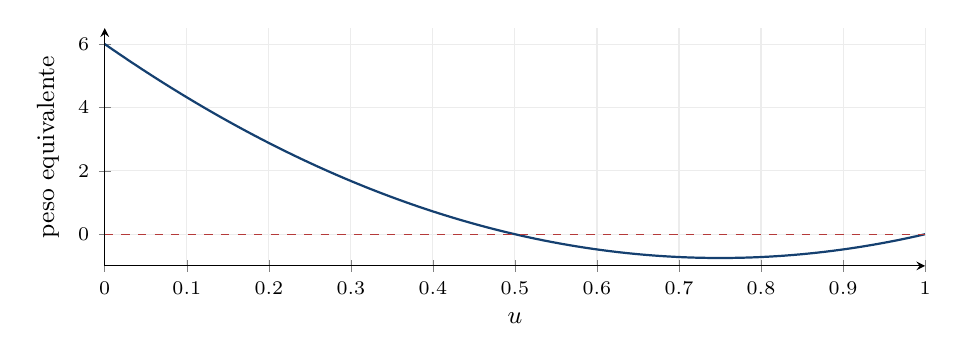
\begin{tikzpicture}\begin{axis}[base,width=12cm,height=4.6cm,xmin=0,xmax=1,ymin=-1,ymax=6.5,xlabel={$u$},ylabel={peso equivalente}]
\addplot[azul,thick,domain=0:1]{6-18*x+12*x^2};\addplot[rojo,dashed] coordinates {(0,0)(1,0)};
\end{axis}\end{tikzpicture}
\caption{Peso equivalente de extrapolación; puede ser negativo aun con kernel triangular positivo.}
\end{figure}

\clearpage
\section{Sesgo de la recta local: conservar el término cuadrático de Taylor}\label{unidad33}
Sea la media lateral suficientemente suave.
En el lado derecho se expande
\[
\begin{aligned}
\E[Y_i\mid x_{i2}=c+hu]
={}&\E[Y_i\mid x_{i2}=c+]\\
&+hu\,\frac{\dd}{\dd x}\E[Y_i\mid x_{i2}=x]\bigg|_{c+}\\
&+\frac{h^2u^2}{2}
\frac{\dd^2}{\dd x^2}\E[Y_i\mid x_{i2}=x]\bigg|_{c+}
+o(h^2).
\end{aligned}
\]
Integrar con la función equivalente anterior
conserva el término constante y anula el lineal.
Como su segundo momento es \(-1/10\),
el sesgo del intercepto derecho es
\[
-\frac{h^2}{20}
\frac{\dd^2}{\dd x^2}\E[Y_i\mid x_{i2}=x]\bigg|_{c+}
+o(h^2).
\]
La reflexión del lado izquierdo conserva
el momento cuadrático, por lo que da
el mismo factor con su curvatura lateral.

Restar los dos interceptos produce
\[
\begin{aligned}
\E[\widehat\tau]-\tau
={}&-\frac{h^2}{20}\left[
\frac{\dd^2}{\dd x^2}\E[Y_i\mid x_{i2}=x]\bigg|_{c+}
-\frac{\dd^2}{\dd x^2}\E[Y_i\mid x_{i2}=x]\bigg|_{c-}
\right]\\
&+o(h^2).
\end{aligned}
\]
El resultado presupone el kernel triangular,
una densidad positiva continua en el corte
y condiciones de aproximación local.
No es una identidad de sesgo finito
para cualquier conjunto de puntajes.

\begin{ejemplo}[Curvatura diferencial]
Si las segundas derivadas son cuatro
a la derecha y uno a la izquierda,
el sesgo principal es \(-3h^2/20\).
Para \(h=.5\), vale \(-.0375\).
\end{ejemplo}
Curvaturas iguales pueden cancelar el
término principal del salto,
aunque cada intercepto esté sesgado.
Eso no garantiza que desaparezcan
los términos de orden mayor.

La especificación global de un polinomio
alto no es necesaria para este argumento:
se utiliza una expansión local en cada lado.
El resto tiene que controlarse
al elegir una banda y hacer inferencia.

\clearpage
\section{Varianza asintótica local: integrar el cuadrado del peso}\label{unidad34}
El intercepto derecho aproxima una combinación
de respuestas con coeficiente
\[
\frac{1}{nh f(c)}
\left[6-18\frac{x_{i2}-c}{h}
+12\left(\frac{x_{i2}-c}{h}\right)^2\right]
\]
para las observaciones del lado derecho
dentro de la banda.
Aquí \(f(c)>0\) es la densidad
del dato de asignación en el corte.

Con varianza condicional continua hacia
ese lado, la suma de cuadrados
de coeficientes produce
\[
\frac{\sigma_+^2}{nhf(c)}
\int_0^1(6-18u+12u^2)^2\dd u.
\]
Expandir el cuadrado da
\(36(1-6u+13u^2-12u^3+4u^4)\).
Su integral es
\[
36\left[1-3+\frac{13}{3}-3+\frac45\right]
=\frac{24}{5}.
\]
El intercepto izquierdo tiene el mismo
factor con su varianza lateral.

Con independencia entre respuestas,
la varianza principal del salto es
\[
\Var(\widehat\tau)
=\frac{24(\sigma_+^2+\sigma_-^2)}
{5nhf(c)}+o((nh)^{-1}).
\]
Si la densidad tiene límites distintos,
se mantienen sus dos densidades
en los términos de cada lado.
La fórmula con un solo \(f(c)\)
necesita continuidad de esa densidad.

El tamaño local efectivo crece como \(nh\).
Reducir \(h\) trae puntos más próximos
y disminuye sesgo, pero deja menos información
para estimar los interceptos.
Por eso el error estándar crece
al reducir demasiado la banda.

\begin{ejemplo}[Escala]
Duplicar \(n\) con \(h\) fijo
divide esta varianza por dos.
Dividir \(h\) por dos con \(n\) fijo
la multiplica por dos en su aproximación principal.
\end{ejemplo}
La fórmula es asintótica.
En una muestra concreta se calculan
pesos y covarianzas con los puntajes realmente observados,
en lugar de sustituirlos mecánicamente
por una integral continua.

\clearpage
\section{Ancho de banda: minimizar el error cuadrático principal}\label{unidad35}
Para la recta local triangular, el sesgo principal
es una constante por \(h^2\), y la varianza
una constante positiva por \(1/(nh)\).
Su error cuadrático principal se escribe
\[
\frac{h^4}{400}
\left[
\frac{\dd^2}{\dd x^2}\E[Y_i\mid x_{i2}=x]\bigg|_{c+}
-\frac{\dd^2}{\dd x^2}\E[Y_i\mid x_{i2}=x]\bigg|_{c-}
\right]^2
+\frac{24(\sigma_+^2+\sigma_-^2)}{5nhf(c)}.
\]
Derivar respecto de \(h>0\) produce
\[
\begin{aligned}
&\frac{h^3}{100}
\left[
\frac{\dd^2}{\dd x^2}\E[Y_i\mid x_{i2}=x]\bigg|_{c+}
-\frac{\dd^2}{\dd x^2}\E[Y_i\mid x_{i2}=x]\bigg|_{c-}
\right]^2\\
&-\frac{24(\sigma_+^2+\sigma_-^2)}{5nh^2f(c)}.
\end{aligned}
\]
Igualar a cero muestra que \(h^5\)
es proporcional a \(1/n\), si la
diferencia de curvaturas no es cero.
Por ello el orden óptimo es \(n^{-1/5}\).
El mínimo equilibra dos errores distintos.

Si la curvatura diferencial se anula,
este cálculo de primer orden no identifica
una banda óptima mediante la misma expresión:
hay que estudiar términos de sesgo posteriores.
No se divide por cero y se llama
óptima a una banda infinita.

Las constantes contienen densidad,
varianzas y derivadas desconocidas.
Un selector práctico debe estimarlas
con procedimientos piloto y suficiente estabilidad.
La tasa sola no determina un número
de puntos o una distancia universal.

\begin{ejemplo}[Dos componentes simples]
Para error principal \(h^4+1/(nh)\),
la derivada es \(4h^3-1/(nh^2)\).
La raíz cumple \(h=(4n)^{-1/5}\).
Con \(n=1000\), aproximadamente .190365.
\end{ejemplo}
Esta optimización busca precisión del estimador puntual.
No garantiza automáticamente cobertura
de un intervalo centrado sin corrección de sesgo.
La escala del sesgo respecto del error estándar
debe estudiarse separadamente.

\begin{figure}[H]\centering
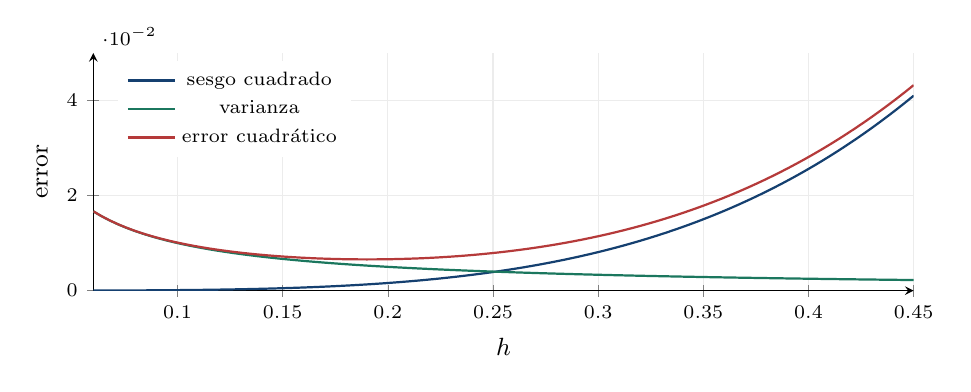
\begin{tikzpicture}\begin{axis}[base,width=12cm,height=4.6cm,xmin=.06,xmax=.45,ymin=0,ymax=.05,xlabel={$h$},ylabel={error},legend pos=north west]
\addplot[azul,thick,domain=.06:.45]{x^4};\addplot[verde,thick,domain=.06:.45]{1/(1000*x)};\addplot[rojo,thick,domain=.06:.45]{x^4+1/(1000*x)};\legend{sesgo cuadrado,varianza,error cuadrático}
\end{axis}\end{tikzpicture}
\caption{Sesgo cuadrado, varianza y su suma en el ejemplo \(h^4+1/(1000h)\).}
\end{figure}

\clearpage
\section{Por qué el ancho óptimo de estimación puede sesgar un intervalo}\label{unidad36}
El sesgo de la recta local tiene orden \(h^2\).
El error estándar tiene orden \((nh)^{-1/2}\).
Su cociente tiene orden
\[
\frac{h^2}{(nh)^{-1/2}}=\sqrt{nh^5}.
\]
Si \(h\) tiene orden \(n^{-1/5}\),
ese cociente puede converger a una constante no nula.
La normal aproximada del estadístico
centrado en el efecto verdadero puede
tener un desplazamiento relevante.

Un intervalo rutinario
\[
\widehat\tau\pm1.95996398\,
\widehat{\mathrm{se}}(\widehat\tau)
\]
controla dispersión, pero no ese desplazamiento.
Estimar varianza robusta a heterocedasticidad
no elimina el sesgo de la media local.

Una solución de subalisado elige una
banda que cumple simultáneamente
\[
h\to0,\qquad nh\to\infty,\qquad nh^5\to0.
\]
La primera reduce aproximación,
la segunda conserva información local
y la tercera hace despreciable
el sesgo de segundo orden frente a la dispersión.
Por ejemplo, \(h=n^{-a}\) con
\(1/5<a<1\) satisface esas tasas
en el caso idealizado correspondiente.

Otra solución estima y resta el sesgo.
Pero la estimación de la curvatura
también es aleatoria.
Su variación y covarianza con el
estimador original tienen que incorporarse.

La inferencia robusta con corrección
de sesgo formaliza esta idea
con polinomios locales y condiciones
de suavidad y banda apropiadas \cite{cct2014}.
El cálculo que sigue mostrará
la propagación por combinaciones lineales
sin presentar la corrección como
una resta determinista.

\begin{ejemplo}[Desplazamiento]
Un sesgo de .05 con error estándar .05
desplaza el centro una desviación estándar.
Aunque ambas cantidades disminuyan al crecer \(n\),
el problema persiste si disminuyen
a la misma tasa.
\end{ejemplo}
No se evalúa cobertura comparando
el número de decimales del estimador.
Se evalúa su distribución centrada
en el parámetro que interesa.

\clearpage
\section{Corrección de sesgo: incluir varianza y covarianza de la curvatura}\label{unidad37}
Con kernel triangular y densidad local continua,
el sesgo principal del salto se estimaría como
\[
-\frac{h^2}{20}\left[
\widehat{\frac{\dd^2}{\dd x^2}\E[Y_i\mid x_{i2}=x]}\bigg|_{c+}
-\widehat{\frac{\dd^2}{\dd x^2}\E[Y_i\mid x_{i2}=x]}\bigg|_{c-}
\right].
\]
Se pueden ajustar cuadráticas laterales
para estimar esas segundas derivadas.
En una cuadrática expresada en \(x_{i2}-c\),
la segunda derivada es dos veces
el coeficiente del término cuadrado.

Restar el sesgo negativo añade
\(h^2/20\) por la diferencia de curvaturas
al salto original.
La varianza de esa suma contiene tres partes:
\[
\begin{aligned}
&\Var(\widehat\tau)
+\frac{h^4}{400}\Var(\text{diferencia estimada de curvaturas})\\
&\qquad+\frac{h^2}{10}
\Cov(\widehat\tau,\text{diferencia estimada de curvaturas}).
\end{aligned}
\]
El signo del cruce proviene de
que aquí se suman las dos cantidades.
Su valor puede ser negativo.
No se omite por utilizar ajustes diferentes:
ambos usan las mismas respuestas.

Condicionado en puntajes y bandas fijos,
cada ajuste polinómico es una
transformación lineal de \(Y\).
Apilar las dos transformaciones permite
calcular su covarianza conjunta
con la misma matriz de errores.
La combinación corregida utiliza
todos los productos cruzados de esas transformaciones.

La expresión \(-1/20\) es una constante
asintótica particular.
Una corrección robusta implementada
puede emplear matrices de momentos
de la muestra y diferentes bandas piloto.
No se afirma que esta sustitución simple
sea una reproducción exacta de cualquier software.

\begin{ejemplo}[Tres componentes]
Si la varianza del salto es .04,
la de la curvatura diferencial es uno,
su covarianza es \(-.1\) y \(h=1\),
la varianza corregida es
\(.04+.0025-.01=.0325\).
\end{ejemplo}
La corrección puede aumentar o disminuir
la varianza por el término cruzado.
Su validez de cobertura requiere además
control del resto de sesgo que queda.

\clearpage
\section{Ajustar covariables: precisión, continuidad y controles posteriores}\label{unidad38}
Se pueden incorporar covariables previas
para mejorar precisión del ajuste.
Considérese la representación
\[
Y_i=\beta_1+\beta_2D_i+\beta_3(x_{i2}-c)
+\beta_4D_i(x_{i2}-c)+\sum_{j=3}^k x_{ij}\eta_j+\varepsilon_i.
\]
Para interpretar \(\beta_2\) como salto
del resultado, se necesita que las
medias de covariables no salten en el corte
bajo los supuestos relevantes.

El contraste observado de la representación es
\[
\beta_2+\sum_{j=3}^k\eta_j\left[
\lim_{x\downarrow c}\E[x_{ij}\mid x_{i2}=x]
-\lim_{x\uparrow c}\E[x_{ij}\mid x_{i2}=x]\right].
\]
Si los saltos de covariables son cero,
queda \(\beta_2\).
Si no son cero, el coeficiente ajustado
y el salto marginal corresponden
a cantidades distintas.

Una variable determinada después del tratamiento
puede ser una vía de su efecto.
Condicionar en ella cambia la pregunta causal
y puede inducir otros sesgos.
No se agrega únicamente porque
su correlación con el resultado sea alta.

La precisión mejora cuando se explica
variación de resultados sin comprometer
la identificación del contraste.
Cada columna extra también exige
rango y suficientes filas locales.
En una banda pequeña, demasiados controles
pueden hacer inestable el sistema.

\begin{ejemplo}[Covariable continua]
Si una covariable previa tiene media
\(1+.2(x-c)\) a ambos lados,
su salto es cero aunque su pendiente no lo sea.
Una covariable con medias uno y dos
en el corte no cumple esa continuidad.
\end{ejemplo}
Un diagnóstico de balance puede ajustar
la misma discontinuidad usando cada
covariable previa como respuesta.
La ausencia de un salto estadísticamente detectable
no demuestra ausencia de todos los
confusores o suficiente potencia.

La metodología de ajuste de covariables
en diseños locales tiene condiciones
propias de identificación e inferencia.
El álgebra muestra qué salto se está
comparando antes de elegir controles.

\clearpage
\section{Manipulación del puntaje: densidad y selección alrededor del corte}\label{unidad39}
La regla conocida no garantiza validez causal.
Si individuos pueden colocarse deliberadamente
a un lado del umbral según características
no observadas, las medias potenciales
pueden dejar de ser continuas.

La densidad del puntaje aporta un diagnóstico:
\[
\lim_{x\downarrow c}f_{x_{i2}}(x)
-\lim_{x\uparrow c}f_{x_{i2}}(x).
\]
Un salto puede ser consistente con
clasificación estratégica, reglas de redondeo
u otros mecanismos.
Su ausencia tampoco demuestra
continuidad de resultados potenciales.

Contar puntos en dos intervalos
de ancho \(h\) aproxima probabilidades:
\[
\Prob(c\le x_{i2}<c+h)
=\int_c^{c+h}f_{x_{i2}}(x)\dd x.
\]
Dividir por \(h\) y llevarlo a cero
recupera la densidad lateral
bajo continuidad dentro de ese lado.
Un conteo bruto no se interpreta
como densidad sin considerar
ancho de intervalos y tamaño de muestra.

\begin{ejemplo}[Clasificación estratégica]
Si personas con motivación alta
pueden subir justo al corte,
el promedio de motivación puede saltar.
Un salto del resultado reflejaría
tratamiento y composición simultáneamente.
\end{ejemplo}
Se estudian también reglas administrativas,
heaping, valores repetidos y discontinuidades
de covariables previas.
Son evidencias sobre mecanismos concretos,
no certificados automáticos de causalidad.

Excluir registros muy próximos al corte
puede intentar abordar ciertos problemas,
pero introduce extrapolación desde más lejos.
No restituye por sí solo la información
que se ha perdido.

La formulación causal requiere que
las otras determinantes relevantes
no produzcan un salto propio en el mismo punto.
Una gráfica visualmente limpia
no sustituye esa discusión institucional
ni las condiciones matemáticas de identificación.

\clearpage
\section{Puntaje discreto: por qué continuidad sola puede no identificar el salto}\label{unidad40}
La identificación por límites requiere
observaciones arbitrariamente próximas al corte.
Si el puntaje solo toma enteros y
el corte está entre cero y uno,
los puntos más cercanos pueden
seguir separados por una distancia positiva.

Considérese observar medias en \(x_{i2}=0\)
y \(x_{i2}=1\).
Dos funciones continuas pueden coincidir
con todos los datos observados y tener
valores diferentes en un corte intermedio.
La continuidad por sí sola
no determina la interpolación dentro
de un intervalo sin soporte.

Si se impone una recta con pendiente conocida,
se puede extrapolar.
Si se impone una cota de curvatura,
se pueden construir límites de sesgo.
Pero estas son hipótesis adicionales,
y deben exponerse como tales.

\begin{ejemplo}[Diferencia y pendiente]
Con modelo
\(Y_i=2+x_{i2}+3D_i+\varepsilon_i\),
comparar medias en \(-1\) y \(1\)
produce diferencia cinco:
dos por el cambio de puntaje
y tres por el tratamiento.
La continuidad de la parte lineal
no convierte esa diferencia en tres.
\end{ejemplo}
Con muchos valores distintos cercanos,
la aproximación local puede ser razonable;
con muy pocos puntos de soporte,
la inferencia depende más de
restricciones sobre la función de media.

Agrupar errores por el valor del puntaje
no identifica una función desconocida
entre valores observados.
Una corrección de dispersión y una
restricción de identificación son
operaciones diferentes.

La aleatorización local ofrece otra
formulación si existe un argumento válido
sobre asignación en una ventana discreta.
Sus hipótesis tampoco aparecen automáticamente
por contar varias observaciones
con el mismo puntaje.

El tamaño de muestra total puede ser enorme
y aun así haber poca información
sobre la forma local por escasez
de valores de asignación distintos.

\clearpage
\section{Donut RD: excluir el centro y analizar la extrapolación restante}\label{unidad41}
Un diseño con exclusión central elimina
filas que cumplen \(|x_{i2}-c|<d\),
para alguna distancia \(d>0\).
El ajuste usa puntos en
\[
d\le|x_{i2}-c|\le h.
\]
La predicción en el corte sigue evaluándose
en distancia cero, aunque no haya
puntos cercanos utilizados.

La función de peso completa sería
\[
\left(1-\frac{|x_{i2}-c|}{h}\right)
\mathbf1\{d\le|x_{i2}-c|\le h\}.
\]
Se recalculan las sumas del diseño
con esa selección. Las constantes
del kernel equivalente cambian;
no se conservan automáticamente
las de integración sobre \([0,1]\).

Si \(d\) permanece fijo al aumentar \(n\),
la extrapolación atraviesa una región
sin datos usados de ancho positivo.
La continuidad por sí sola no controla
cuánto puede curvarse la media allí.

\begin{ejemplo}[Un término cuadrático]
Si la media contiene \((x_{i2}-c)^2\),
una recta ajustada desde puntos lejanos
puede llegar a un intercepto sesgado.
Quitar los puntos más próximos
puede aumentar esa sensibilidad.
\end{ejemplo}
Una exclusión central puede ser útil
para estudiar resultados bajo ciertas
reglas de redondeo o clasificación.
Pero cambia el diseño efectivo
y puede requerir hipótesis más fuertes.

La comparación de varios tamaños
de exclusión es un análisis de sensibilidad,
no una prueba de que el resultado
con cualquier exclusión sea causal.
También deben mostrarse los números
de puntos distintos y observaciones
que quedan a cada lado.

La respuesta matemática consiste en
recalcular pesos, sesgo potencial y dispersión.
No basta borrar filas y conservar
los intervalos y argumentos del
diseño original sin revisarlos.

\clearpage
\section{Discontinuidad fuzzy: elegibilidad y tratamiento recibido}\label{unidad42}
En un diseño fuzzy, la elegibilidad \(D_i\)
cambia en el umbral, pero el tratamiento
recibido \(T_i\) no coincide siempre con ella.
Algunas personas elegibles no participan;
algunas no elegibles pueden recibirlo
por otras vías.

Se estudian dos saltos observables:
\[
\begin{aligned}
&\lim_{x\downarrow c}\E[Y_i\mid x_{i2}=x]
-\lim_{x\uparrow c}\E[Y_i\mid x_{i2}=x],\\
&\lim_{x\downarrow c}\E[T_i\mid x_{i2}=x]
-\lim_{x\uparrow c}\E[T_i\mid x_{i2}=x].
\end{aligned}
\]
El segundo es la primera etapa:
el cambio de probabilidad de tratamiento
inducido por cruzar el umbral.

Bajo exclusión, continuidad de los objetos
potenciales relevantes, monotonía y
primera etapa no nula,
la razón de esos dos saltos identifica
un efecto local entre cumplidores.
No es necesariamente el efecto
promedio de toda la población.

\begin{ejemplo}[Saltos observados]
Si la media del resultado salta .6
y la probabilidad de tratamiento salta .3,
la razón es dos.
Dividir por la probabilidad tratada
a la derecha, por ejemplo .8,
calcularía otra cantidad.
\end{ejemplo}
La elegibilidad puede actuar como
instrumento local. Si también cambia
directamente el resultado por otra política,
la exclusión necesaria puede fallar.

Un salto de tratamiento muy pequeño
hace inestable el cociente.
La precisión de los dos saltos
y su covarianza importan.
Una gráfica donde sube algo
la participación no garantiza
una primera etapa fuerte.

Para estimar, se ajustan las mismas
funciones locales a \(y_i\)
y a \(T_i\). La comparación utiliza
puntajes, pesos y bandas compatibles
con la interpretación elegida.
El contraste no se obtiene mezclando
dos poblaciones locales arbitrarias.

\clearpage
\section{Cumplidores: deducir la razón de Wald desde los tipos de tratamiento}\label{unidad43}
Definamos los tratamientos potenciales
\(T_i(0)\) sin elegibilidad y \(T_i(1)\) con ella.
Monotonía exige
\(T_i(1)\ge T_i(0)\).
Los tipos posibles son siempre tratados,
nunca tratados y cumplidores.
La monotonía excluye quienes harían lo contrario.

Bajo exclusión, los resultados potenciales
dependen del tratamiento recibido,
no directamente de la elegibilidad.
Al cambiar elegibilidad, la diferencia es
\[
Y_i(T_i(1))-Y_i(T_i(0))
=(Y_i(1)-Y_i(0))(T_i(1)-T_i(0)).
\]
La identidad se comprueba en los
tres tipos admitidos.
Para siempre y nunca tratados,
el segundo factor vale cero.
Para cumplidores vale uno.

Al promediar localmente en el corte,
el salto de resultados es
\[
\Prob(T_i(1)>T_i(0)\mid x_{i2}=c)
\,\E[Y_i(1)-Y_i(0)\mid T_i(1)>T_i(0),x_{i2}=c].
\]
El salto de tratamiento es
\[
\E[T_i(1)-T_i(0)\mid x_{i2}=c]
=\Prob(T_i(1)>T_i(0)\mid x_{i2}=c).
\]
La continuidad de las distribuciones
potenciales permite conectar esos
contrastes con los límites observables.
Si la probabilidad es positiva,
dividir cancela ese factor común.

\begin{ejemplo}[Composición]
Con .2 siempre tratados, .5 nunca
y .3 cumplidores, la primera etapa es .3.
Si el efecto medio de cumplidores es dos,
el salto de resultados es .6.
No hace falta que el efecto de los
siempre tratados también sea dos.
\end{ejemplo}
Sin monotonía, el denominador mezcla
cumplidores y quienes actúan en sentido contrario.
La razón ya no tiene esta
interpretación simple con pesos positivos.

La derivación explica por qué se
divide por un salto y qué
población aparece en el resultado.
Las condiciones de identificación no
se reemplazan por el nombre
del estimador o por su fórmula.

\clearpage
\section{IV local y razón de saltos: equivalencia algebraica justificada}\label{unidad44}
En una aproximación local, el resultado se modela como
\[
Y_i=\beta_1+\tau T_i+\beta_3(x_{i2}-c)
+\beta_4D_i(x_{i2}-c)+\varepsilon_i.
\]
La elegibilidad \(D_i\) instrumenta \(T_i\).
Las otras tres columnas son controles locales.
El diseño instrumental es
\((1,D_i,x_{i2}-c,D_i(x_{i2}-c))\).

La proyección local de \(T_i\) sobre
esas cuatro columnas tiene un coeficiente
de \(D_i\), que es su salto ajustado.
La proyección del resultado tiene
su propio coeficiente de \(D_i\).
Si la ecuación IV usa exactamente
esas mismas columnas y ponderación,
sus momentos implican que
\[
\text{salto ajustado de resultados}
=\tau\,\text{salto ajustado de tratamiento}.
\]
Los controles tienen salto propio cero
en distancia cero en esta representación.
Con primera etapa no nula,
la solución para \(\tau\) es la razón.

La igualdad es de un sistema local
exactamente identificado con esas columnas.
Agregar instrumentos, imponer pendientes
o utilizar bandas distintas puede
cambiar la equivalencia muestral.
Debe comprobarse en el sistema realmente usado.

Las matrices instrumental por regresor
se construyen con productos como
\[
\sum_i K\left(\frac{x_{i2}-c}{h}\right)D_iT_i,
\quad
\sum_i K\left(\frac{x_{i2}-c}{h}\right)(x_{i2}-c)T_i.
\]
Los controles e interacciones también
aparecen en todas las otras entradas.
No se decide el coeficiente dividiendo
dos productos aislados y omitiendo
el ajuste por esas columnas.

\begin{ejemplo}[Primera etapa perfecta]
Si \(T_i=D_i\), la proyección del tratamiento
tiene salto uno y pendientes cero.
La razón vuelve al salto sharp.
Este límite conecta ambos diseños.
\end{ejemplo}
La equivalencia algebraica no demuestra
exclusión ni monotonía causal.
Esas hipótesis son las que permiten
interpretar el número estimado como
efecto local de cumplidores.

\clearpage
\section{Covarianza del cociente fuzzy: abrir los tres términos}\label{unidad45}
Los saltos de resultado y de tratamiento
se estiman con las mismas filas.
Por eso se necesita su covarianza conjunta.
El método delta de la razón produce
\[
\begin{aligned}
\Var(\widehat\tau_{\mathrm{fuzzy}})
\approx&
\frac{\Var(\text{salto estimado de resultados})}
{(\text{salto de tratamiento})^2}\\
&+\frac{(\text{salto de resultados})^2}
{(\text{salto de tratamiento})^4}
\Var(\text{salto estimado de tratamiento})\\
&-\frac{2\,\text{salto de resultados}}
{(\text{salto de tratamiento})^3}
\Cov(\text{los dos saltos estimados}).
\end{aligned}
\]
En una implementación se sustituyen
los valores estimados bajo condiciones
que permiten esa aproximación.
Cada derivada se evaluó antes de
introducir esos valores.

Para obtener la covarianza entre saltos,
se propagan sus coeficientes lineales
sobre las respuestas \(Y_i,T_i\).
La matriz central contiene
\(\Cov(Y_i,T_i\mid x_i)\) por fila,
además de sus dos varianzas.
No se puede asumir cero simplemente
porque una respuesta sea continua
y la otra binaria.

\begin{ejemplo}[Una cuenta]
Saltos .6 y .3, varianzas .01 y .0025,
y covarianza .003, producen
\[
.01/.09+.36(.0025)/.0081-1.2(.003)/.027
=.08888889.
\]
El error estándar aproximado es
\(\sqrt{.08888889}\approx.29814240\).
\end{ejemplo}
Los intervalos de Wald utilizan
una expansión local en un denominador
que debe ser suficientemente informativo.
Si el salto de tratamiento es pequeño,
la razón puede tener colas largas
y asimetría que la aproximación
no reproduce bien.

La incertidumbre de primera etapa
forma parte del estimador fuzzy.
Considerar fijo su denominador
eliminaría el segundo término y el cruce,
y calcularía otro problema.

\clearpage
\section{Primera etapa débil: invertir una prueba en vez de dividir a ciegas}\label{unidad46}
Para contrastar que el efecto fuzzy
es un valor \(\tau_0\), se puede estudiar
\[
\text{salto de resultados}
-\tau_0\,\text{salto de tratamiento}=0.
\]
Su varianza conjunta es
\[
\begin{aligned}
&\Var(\text{salto estimado de resultados})
+\tau_0^2\Var(\text{salto estimado de tratamiento})\\
&\quad-2\tau_0\Cov(\text{los dos saltos estimados}).
\end{aligned}
\]
No aparece la división por una
primera etapa estimada cerca de cero.

Bajo una aproximación normal conjunta válida
para los saltos, se aceptan los valores que cumplen
\[
\begin{aligned}
&[\text{salto estimado de resultados}
-\tau_0\,\text{salto estimado de tratamiento}]^2\\
&\le1.95996398^2\left[
\begin{gathered}
\Var(\text{salto estimado de resultados})
\\
+\tau_0^2\Var(\text{salto estimado de tratamiento})
\\
-2\tau_0\Cov(\text{los dos saltos estimados})
\end{gathered}
\right].
\end{aligned}
\]
Al expandir, se obtiene una desigualdad
cuadrática en \(\tau_0\).
Su coeficiente de \(\tau_0^2\) contiene
el cuadrado del salto de tratamiento
menos el valor crítico al cuadrado
por su varianza.

Si ese coeficiente no es positivo,
el conjunto de valores aceptados
puede ser no acotado o disjunto.
No es un fallo de presentación:
los datos no limitan suficientemente
la razón en ambas direcciones.

\begin{ejemplo}[Denominador indistinguible de cero]
Un salto de tratamiento .02 con error
estándar .04 admite cero ampliamente.
Un efecto puntual obtenido al dividir
puede cambiar mucho por pequeñas
fluctuaciones de esa primera etapa.
\end{ejemplo}
Este razonamiento es una inversión
de pruebas sobre una combinación lineal,
relacionada con conjuntos de Fieller.
Todavía requiere controlar el sesgo
y la dispersión de los saltos.
No se lo llama exacto para
cualquier ajuste no paramétrico pequeño.

\clearpage
\section{Regression kink: distinguir un salto de nivel de un cambio de pendiente}\label{unidad47}
Una política puede ser continua en el corte,
pero cambiar su pendiente.
Entonces el tratamiento no necesariamente
presenta un salto de nivel.
Un diseño de kink estudia
derivadas laterales de medias:
\[
\frac{\dd}{\dd x}\E[Y_i\mid x_{i2}=x]\bigg|_{c+}
-
\frac{\dd}{\dd x}\E[Y_i\mid x_{i2}=x]\bigg|_{c-}.
\]
No debe confundirse con la diferencia
de los niveles laterales.

En la representación de rectas,
\(\beta_2\) es salto de nivel
y \(\beta_4\) cambio de pendiente.
Imponer \(\beta_2=0\) describe
una función continua con posible kink.
Las dos restricciones son distintas.

Si una intensidad de política conocida
cambia de pendiente y el resultado
se relaciona causalmente con esa intensidad,
una razón de cambios de pendiente
puede identificar una respuesta causal
bajo hipótesis adicionales específicas.
No se obtiene esa interpretación
de una derivada visual sin discutir
exclusión, suavidad y composición.

\begin{ejemplo}[Función continua]
\(Y=2+.5(x-c)+.8D(x-c)\) es continua.
La pendiente pasa de .5 a 1.3,
por lo que el cambio es .8.
El salto de nivel es cero.
\end{ejemplo}
Estimar derivadas es más exigente
que estimar niveles.
El orden de varianza local depende
de la potencia del ancho de banda:
una derivada de primer orden
tiene típicamente escala \(1/(nh^3)\)
en vez de \(1/(nh)\).

El polinomio local debe tener orden
suficiente para aproximar esa derivada,
y el sesgo se desarrolla con
derivadas superiores de la media.
Un intervalo diseñado para un salto
de niveles no se recicla sin
ajustar esa escala y la matriz
que selecciona la pendiente.

\begin{figure}[H]\centering
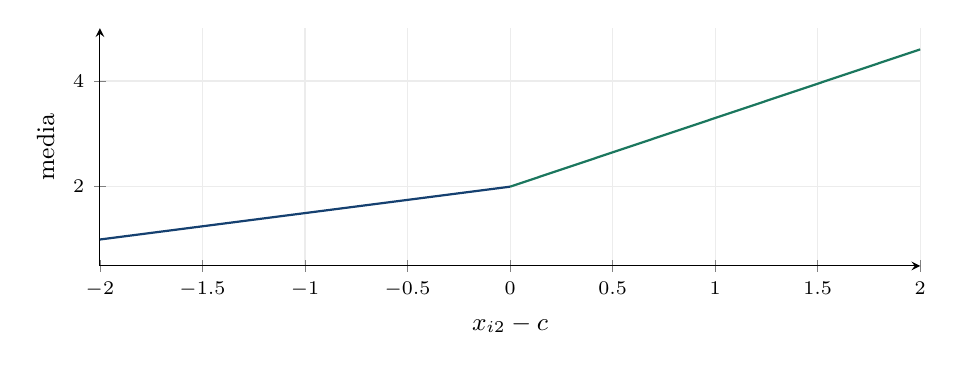
\begin{tikzpicture}\begin{axis}[base,width=12cm,height=4.6cm,xmin=-2,xmax=2,ymin=.5,ymax=5,xlabel={$x_{i2}-c$},ylabel={media}]
\addplot[azul,thick,domain=-2:0]{2+.5*x};\addplot[verde,thick,domain=0:2]{2+1.3*x};
\end{axis}\end{tikzpicture}
\caption{Una función continua con pendiente distinta a cada lado; el nivel no salta.}
\end{figure}

\clearpage
\section{Aleatorización local: construir una prueba por asignaciones}\label{unidad48}
Un enfoque diferente supone que, en una ventana
especificada, la asignación responde
a un mecanismo de aleatorización.
Con un número fijo de tratados,
pueden enumerarse todas las asignaciones
admitidas por ese mecanismo.

Bajo la hipótesis nula sharp de
efecto cero para cada individuo,
todos los resultados potenciales
observados bajo cualquier asignación
son los mismos números.
Se puede entonces recalcular
una diferencia de medias
para cada asignación posible.

Con cuatro individuos y dos tratados,
hay \(\binom42=6\) asignaciones.
Si todas son igualmente probables,
el valor p bilateral es la fracción
cuyos estadísticos absolutos son
al menos el observado.
No se exige una aproximación normal
para esa distribución finita.

\begin{ejemplo}[Cuatro resultados]
Con resultados \(1,2,3,4\)
y tratados los dos mayores,
la diferencia de medias es dos.
Las seis diferencias son
\(-2,-1,0,0,1,2\).
Dos tienen valor absoluto al menos dos,
por lo que el valor p es \(2/6\).
\end{ejemplo}
La validez depende del mecanismo
de asignación supuesto dentro de
esa ventana y de la hipótesis sharp.
No se pueden permutar etiquetas
en cualquier discontinuidad solo
porque los puntos estén cerca.

En el marco de continuidad,
la asignación es determinista
dado el puntaje observado.
Una prueba por permutaciones
requiere la formulación adicional
de aleatorización local correspondiente.

La elección de ventana debe
ser coherente con las hipótesis.
Buscar muchas ventanas y reportar
solo la que produce menor valor p
cambia el procedimiento de inferencia.

Se distinguirán resultados bajo
continuidad de resultados bajo
aleatorización local en las
interpretaciones del tratado.
Ambos enfoques pueden ser útiles,
pero necesitan argumentos distintos.

\clearpage
\section{Varios umbrales, tiempo y fronteras: identificar qué comparación se conserva}\label{unidad49}
Algunas reglas usan varios cortes.
Para un individuo sujeto al corte \(c_g\),
la distancia relevante es \(x_{i2}-c_g\).
Apilar esas distancias combina
poblaciones y potencialmente
efectos locales distintos.

Un promedio de saltos de varios cortes
requiere declarar sus pesos y qué
efecto agregado se busca.
Un coeficiente común impone
homogeneidad o una proyección
que no debe confundirse con
cada efecto local por separado.

Si el puntaje es tiempo,
otras variables pueden cambiar
en la misma fecha por tendencias,
estacionalidad o shocks.
Las unidades antes y después
pueden tener dependencia temporal.
Un corte conocido en fecha
no garantiza la validez de
un diseño causal de discontinuidad.

En una frontera geográfica, la
distancia al límite puede parecer
un puntaje de asignación.
La continuidad de características,
el movimiento estratégico y los
efectos de vecindad requieren
consideración especial.
La posición en una dimensión
no describe necesariamente toda
la heterogeneidad espacial.

\begin{ejemplo}[Dos políticas]
Si una beca y un beneficio adicional
comienzan en el mismo puntaje,
el salto puede representar
su cambio conjunto.
Separarlos exige otra fuente
de variación o hipótesis adicional.
\end{ejemplo}
La fórmula de resta lateral
se conserva algebraicamente,
pero su interpretación depende
de qué tratamientos y poblaciones
cambian a ambos lados.

Una extensión del diseño no
se valida simplemente conservando
el nombre RD.
Hay que reconstruir resultados
potenciales, regla de asignación,
condiciones de continuidad
y estructura de errores
para la comparación concreta.

\clearpage
\section{Laboratorio RD: dieciséis datos y todas las columnas del diseño}\label{unidad50}
Fijemos \(c=0,h=4\).
Las filas contienen puntaje, elegibilidad y resultado
didáctico. La columna de interacción se calcula
multiplicando elegibilidad por puntaje centrado.
La tabla muestra todas las entradas del diseño,
la respuesta y el peso utilizado.
\begin{center}\small\begin{tabular}{rrrrrrr}\toprule
\(i\)&\(1\)&\(D_i\)&\(x_{i2}-c\)&\(D_i(x_{i2}-c)\)&\(y_i\)&\(1-|x_{i2}-c|/4\)\\\midrule
1&1&0&-4.0&-0.0&-0.200&0.000\\
2&1&0&-3.5&-0.0&0.350&0.125\\
3&1&0&-3.0&-0.0&0.500&0.250\\
4&1&0&-2.5&-0.0&1.050&0.375\\
5&1&0&-2.0&-0.0&0.900&0.500\\
6&1&0&-1.5&-0.0&1.450&0.625\\
7&1&0&-1.0&-0.0&1.300&0.750\\
8&1&0&-0.5&-0.0&1.850&0.875\\
9&1&1&0.5&0.5&5.400&0.875\\
10&1&1&1.0&1.0&6.200&0.750\\
11&1&1&1.5&1.5&6.300&0.625\\
12&1&1&2.0&2.0&7.300&0.500\\
13&1&1&2.5&2.5&7.500&0.375\\
14&1&1&3.0&3.0&7.900&0.250\\
15&1&1&3.5&3.5&8.700&0.125\\
16&1&1&4.0&4.0&8.800&0.000\\\bottomrule\end{tabular}\end{center}
Los extremos \(-4,4\) tienen peso cero.
Quedan siete puntajes de peso positivo por lado.
Las rectas locales usan las cuatro columnas
en las mismas dieciséis filas; el peso cero
hace que los extremos no alteren el mínimo.

Para estudiar momentos exactos, el mecanismo
de referencia de este laboratorio es
\[
Y_i=2+3D_i+.5x_{i2}+.5D_ix_{i2}+\varepsilon_i,
\qquad \varepsilon_i\overset{\mathrm{ind}}{\sim}\mathcal N(0,.25).
\]
La tabla constituye una realización didáctica.
Los coeficientes verdaderos de referencia son
\((2,3,.5,.5)\T\).
Se distinguirán sus momentos condicionados
de los coeficientes que resultan de esta tabla.

Las filas con elegibilidad cero no contribuyen
a los productos que incluyen \(D_i\).
Las del otro lado contribuyen
a todos esos productos.
Los productos con \(x_{i2}\) conservan
su signo; los cuadrados son no negativos.

La discontinuidad de referencia es tres.
La diferencia de pendientes es .5.
No se estima el salto promediando
todos los resultados derechos menos
todos los izquierdos: también se ajusta
por la distancia al umbral.

\begin{figure}[H]\centering
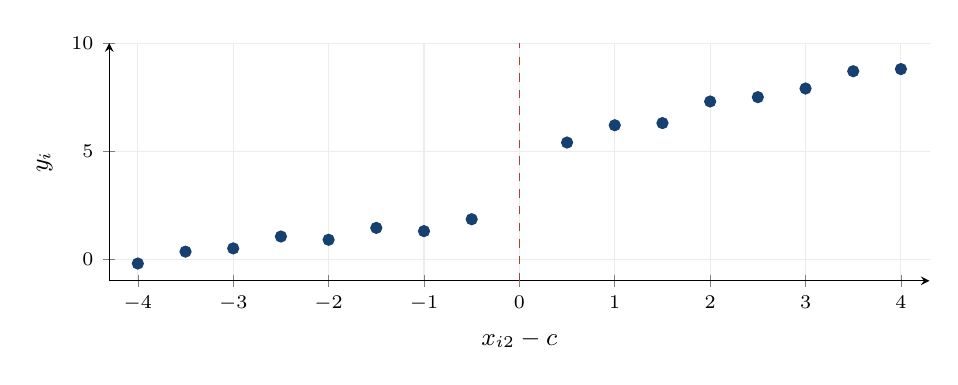
\begin{tikzpicture}\begin{axis}[base,width=12cm,height=4.6cm,xmin=-4.3,xmax=4.3,ymin=-1,ymax=10,xlabel={$x_{i2}-c$},ylabel={$y_i$}]
\addplot[only marks,mark=*,azul] coordinates {(-4.00,-0.2000) (-3.50,0.3500) (-3.00,0.5000) (-2.50,1.0500) (-2.00,0.9000) (-1.50,1.4500) (-1.00,1.3000) (-0.50,1.8500) (0.50,5.4000) (1.00,6.2000) (1.50,6.3000) (2.00,7.3000) (2.50,7.5000) (3.00,7.9000) (3.50,8.7000) (4.00,8.8000)};\addplot[rojo,dashed] coordinates {(0,-1)(0,10)};
\end{axis}\end{tikzpicture}
\caption{Dieciséis resultados del laboratorio; cada recta se extrapola hacia el corte.}
\end{figure}

\clearpage
\section{Laboratorio RD: cinco sumas y recta del lado izquierdo}\label{unidad51}
La selección de esta unidad conserva únicamente el lado izquierdo.
Para cada fila se evalúa \(K=1-|x_{i2}|/4\) dentro de la banda.
Las sumas a continuación están abiertas en los ocho
datos de ese lado, incluyendo el peso cero extremo.
La función del kernel se mostró completa en la tabla;
en estas etiquetas la letra \(K\) designa esa función evaluada.
\[
\begin{aligned}
\sum K&=(0.000000)+(0.125000)+(0.250000)+(0.375000)\\&\quad+(0.500000)+(0.625000)+(0.750000)+(0.875000)\\&=3.50000000.\end{aligned}
\]
\[
\begin{aligned}
\sum K(x_{i2}-c)&=(-0.000000)+(-0.437500)+(-0.750000)+(-0.937500)\\&\quad+(-1.000000)+(-0.937500)+(-0.750000)+(-0.437500)\\&=-5.25000000.\end{aligned}
\]
\[
\begin{aligned}
\sum K(x_{i2}-c)^2&=(0.000000)+(1.531250)+(2.250000)+(2.343750)\\&\quad+(2.000000)+(1.406250)+(0.750000)+(0.218750)\\&=10.50000000.\end{aligned}
\]
\[
\begin{aligned}
\sum Ky_i&=(-0.000000)+(0.043750)+(0.125000)+(0.393750)\\&\quad+(0.450000)+(0.906250)+(0.975000)+(1.618750)\\&=4.51250000.\end{aligned}
\]
\[
\begin{aligned}
\sum K(x_{i2}-c)y_i&=(0.000000)+(-0.153125)+(-0.375000)+(-0.984375)\\&\quad+(-0.900000)+(-1.359375)+(-0.975000)+(-0.809375)\\&=-5.55625000.\end{aligned}
\]

Las tres primeras sumas forman la matriz de la recta.
Las últimas dos forman el lado derecho:
\[
\begin{pmatrix}3.5000000&-5.2500000\\-5.2500000&10.5000000\end{pmatrix}\begin{pmatrix}\text{intercepto}\\\text{pendiente}\end{pmatrix}=\begin{pmatrix}4.5125000\\-5.5562500\end{pmatrix}.
\]

Su determinante es positivo:
\[
(3.50000000)(10.50000000)-(-5.25000000)^2=9.18750000.
\]

Eliminación o inversión de dos por dos produce
\[
\begin{pmatrix}\text{intercepto}\\\text{pendiente}\end{pmatrix}\approx\begin{pmatrix}1.9821429\\0.4619048\end{pmatrix}.
\]

Multiplicar la matriz por ese vector recupera
el lado derecho salvo redondeo.
El intercepto representa el valor extrapolado
a distancia cero, incluso si no hay una
observación exactamente en el corte.

El cálculo no decide la interpretación causal:
esta depende de las hipótesis de continuidad
desarrolladas antes. Aquí se verifica
la operación algebraica sobre datos explícitos.

\clearpage
\section{Laboratorio RD: cinco sumas y recta del lado derecho}\label{unidad52}
La selección de esta unidad conserva únicamente el lado derecho.
Para cada fila se evalúa \(K=1-|x_{i2}|/4\) dentro de la banda.
Las sumas a continuación están abiertas en los ocho
datos de ese lado, incluyendo el peso cero extremo.
La función del kernel se mostró completa en la tabla;
en estas etiquetas la letra \(K\) designa esa función evaluada.
\[
\begin{aligned}
\sum K&=(0.875000)+(0.750000)+(0.625000)+(0.500000)\\&\quad+(0.375000)+(0.250000)+(0.125000)+(0.000000)\\&=3.50000000.\end{aligned}
\]
\[
\begin{aligned}
\sum K(x_{i2}-c)&=(0.437500)+(0.750000)+(0.937500)+(1.000000)\\&\quad+(0.937500)+(0.750000)+(0.437500)+(0.000000)\\&=5.25000000.\end{aligned}
\]
\[
\begin{aligned}
\sum K(x_{i2}-c)^2&=(0.218750)+(0.750000)+(1.406250)+(2.000000)\\&\quad+(2.343750)+(2.250000)+(1.531250)+(0.000000)\\&=10.50000000.\end{aligned}
\]
\[
\begin{aligned}
\sum Ky_i&=(4.725000)+(4.650000)+(3.937500)+(3.650000)\\&\quad+(2.812500)+(1.975000)+(1.087500)+(0.000000)\\&=22.83750000.\end{aligned}
\]
\[
\begin{aligned}
\sum K(x_{i2}-c)y_i&=(2.362500)+(4.650000)+(5.906250)+(7.300000)\\&\quad+(7.031250)+(5.925000)+(3.806250)+(0.000000)\\&=36.98125000.\end{aligned}
\]

Las tres primeras sumas forman la matriz de la recta.
Las últimas dos forman el lado derecho:
\[
\begin{pmatrix}3.5000000&5.2500000\\5.2500000&10.5000000\end{pmatrix}\begin{pmatrix}\text{intercepto}\\\text{pendiente}\end{pmatrix}=\begin{pmatrix}22.8375000\\36.9812500\end{pmatrix}.
\]

Su determinante es positivo:
\[
(3.50000000)(10.50000000)-(5.25000000)^2=9.18750000.
\]

Eliminación o inversión de dos por dos produce
\[
\begin{pmatrix}\text{intercepto}\\\text{pendiente}\end{pmatrix}\approx\begin{pmatrix}4.9678571\\1.0380952\end{pmatrix}.
\]

Multiplicar la matriz por ese vector recupera
el lado derecho salvo redondeo.
El intercepto representa el valor extrapolado
a distancia cero, incluso si no hay una
observación exactamente en el corte.

El cálculo no decide la interpretación causal:
esta depende de las hipótesis de continuidad
desarrolladas antes. Aquí se verifica
la operación algebraica sobre datos explícitos.

\clearpage
\section{Laboratorio RD: ensamblar el sistema de cuatro coeficientes}\label{unidad53}
Sumar los productos exteriores de todas las filas
con su peso triangular produce la matriz
mostrada aquí. Sus entradas corresponden
a las sumas de la matriz general de cuatro columnas:
\[
\sum_i\left(1-\frac{|x_{i2}|}{4}\right)
\begin{pmatrix}1\\D_i\\x_{i2}\\D_ix_{i2}\end{pmatrix}
(1,D_i,x_{i2},D_ix_{i2})
=\begin{pmatrix}7.0000000&3.5000000&0&5.2500000\\3.5000000&3.5000000&5.2500000&5.2500000\\0&5.2500000&21.0000000&10.5000000\\5.2500000&5.2500000&10.5000000&10.5000000\end{pmatrix}.
\]

El vector derecho suma cada columna por
el resultado y el mismo peso:
\[
\sum_i\left(1-\frac{|x_{i2}|}{4}\right)
\begin{pmatrix}y_i\\D_iy_i\\x_{i2}y_i\\D_ix_{i2}y_i\end{pmatrix}
=\begin{pmatrix}27.3500000\\22.8375000\\31.4250000\\36.9812500\end{pmatrix}.
\]

Resolver el sistema completo da
\[
\widehat\beta=\begin{pmatrix}1.9821429\\2.9857143\\0.4619048\\0.5761905\end{pmatrix}.
\]

Las rectas estimadas son
\[
\begin{aligned}
\text{izquierda}:\quad&1.98214286+(0.46190476)x_{i2},\\\text{derecha}:\quad&4.96785714+(1.03809524)x_{i2}.\end{aligned}
\]

El salto es la segunda coordenada.
La diferencia de pendientes es la cuarta.
Ambos resultados coinciden con restar
las soluciones de las rectas laterales,
porque se usaron los mismos datos y pesos.

Los coeficientes tienen esperanza de referencia
\((2,3,.5,.5)\T\) bajo el modelo lineal
normal del laboratorio.
La diferencia de esta realización respecto
de esos valores proviene de sus errores.

El sistema tiene dimensión cuatro,
aunque haya dieciséis respuestas.
Ninguna coordenada se calcula ignorando
las otras tres: el producto cruzado
mezcla intercepto, elegibilidad y pendientes.

\begin{figure}[H]\centering
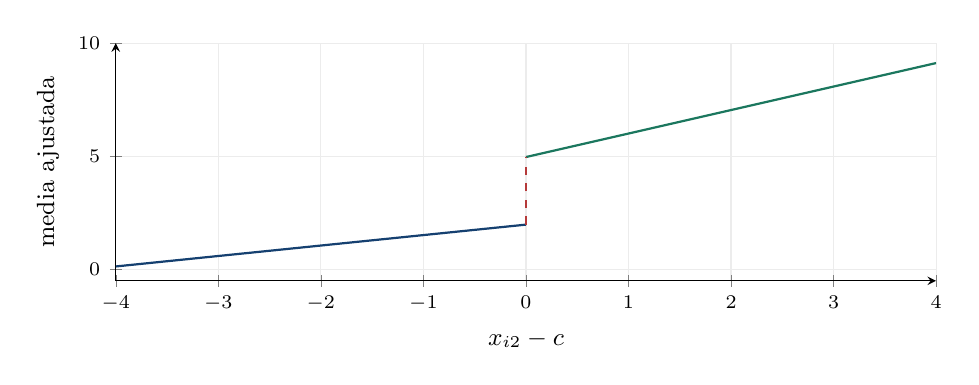
\begin{tikzpicture}\begin{axis}[base,width=12cm,height=4.6cm,xmin=-4,xmax=4,ymin=-.5,ymax=10,xlabel={$x_{i2}-c$},ylabel={media ajustada}]
\addplot[azul,thick,domain=-4:0]{1.9821428571+(0.4619047619)*x};\addplot[verde,thick,domain=0:4]{4.9678571429+(1.0380952381)*x};\addplot[rojo,dashed] coordinates {(0,1.9821428571)(0,4.9678571429)};
\end{axis}\end{tikzpicture}
\caption{Rectas estimadas del laboratorio y contraste en el corte.}
\end{figure}

\clearpage
\section{Laboratorio RD: las dieciséis contribuciones al salto}\label{unidad54}
La solución de cuadrados es lineal en las respuestas.
La segunda fila de la matriz que las multiplica
contiene los coeficientes de cada \(y_i\)
en el salto estimado. Se muestran sin omitir
las filas con coeficiente cero.
\begin{center}\small\begin{tabular}{rrrr}\toprule
\(i\)&\(x_{i2}\)&coeficiente de \(y_i\)&coeficiente por \(y_i\)\\\midrule
1&-4.00&0.000000000&-0.000000000\\
2&-3.50&0.107142857&0.037500000\\
3&-3.00&0.142857143&0.071428571\\
4&-2.50&0.107142857&0.112500000\\
5&-2.00&-0.000000000&-0.000000000\\
6&-1.50&-0.178571429&-0.258928571\\
7&-1.00&-0.428571429&-0.557142857\\
8&-0.50&-0.750000000&-1.387500000\\
9&0.50&0.750000000&4.050000000\\
10&1.00&0.428571429&2.657142857\\
11&1.50&0.178571429&1.125000000\\
12&2.00&0.000000000&0.000000000\\
13&2.50&-0.107142857&-0.803571429\\
14&3.00&-0.142857143&-1.128571429\\
15&3.50&-0.107142857&-0.932142857\\
16&4.00&0.000000000&0.000000000\\\bottomrule\end{tabular}\end{center}
Sumar los productos de la última columna da
\[
\begin{aligned}
\widehat\tau&\approx(-0.0000000)+(0.0375000)+(0.0714286)+(0.1125000)\\&\quad+(-0.0000000)+(-0.2589286)+(-0.5571429)+(-1.3875000)\\&\quad+(4.0500000)+(2.6571429)+(1.1250000)+(0.0000000)\\&\quad+(-0.8035714)+(-1.1285714)+(-0.9321429)+(0.0000000)\\&=2.985714286.\end{aligned}
\]

Esa fila reproduce el salto de la representación:
sus coeficientes por la columna constante suman cero;
por \(D_i\), suman uno;
por \(x_{i2}\), suman cero;
por \(D_ix_{i2}\), suman cero.
Estas cuatro identidades comprueban que elimina
los otros tres términos de una recta lateral correcta.

Con errores independientes de varianza .25,
la varianza del salto es la suma
de cuadrados de esos coeficientes por .25:
\[
.25\sum_i(\text{coeficiente de }y_i)^2=0.4107142857.
\]

Los coeficientes de respuestas alejadas
pueden ser negativos. No son probabilidades;
se usan para extrapolar una recta
al punto donde se evalúa el contraste.
La suma por lado tiene signo propio:
uno para el derecho y menos uno
para el izquierdo.

Este cálculo verifica la misma varianza
que se obtendrá con las tres matrices
de propagación. La igualdad de ambos
procedimientos es una comprobación algebraica,
no una hipótesis de independencia
entre coeficientes estimados.

\clearpage
\section{Laboratorio RD: covarianza completa e intervalo del salto}\label{unidad55}
Bajo varianza conocida .25 del mecanismo de referencia,
la matriz central usa el cuadrado de cada peso:
\[
.25\sum_i\left(1-\frac{|x_{i2}|}{4}\right)^2
\begin{pmatrix}1\\D_i\\x_{i2}\\D_ix_{i2}\end{pmatrix}
(1,D_i,x_{i2},D_ix_{i2})
=\begin{pmatrix}1.0937500&0.5468750&0&0.6562500\\0.5468750&0.5468750&0.6562500&0.6562500\\0&0.6562500&2.1328125&1.0664062\\0.6562500&0.6562500&1.0664062&1.0664062\end{pmatrix}.
\]

Multiplicar a ambos lados por la inversa
de la matriz normal local produce
\[
\Cov(\widehat\beta\mid X)=\begin{pmatrix}0.2053571&-0.2053571&0.0892857&-0.0892857\\-0.2053571&0.4107143&-0.0892857&0\\0.0892857&-0.0892857&0.0476190&-0.0476190\\-0.0892857&0&-0.0476190&0.0952381\end{pmatrix}.
\]

Se conservan las dieciséis entradas.
Las raíces de la diagonal son
los errores estándar de las cuatro coordenadas:
\[
\begin{pmatrix}0.4531635\\0.6408699\\0.2182179\\0.3086067\end{pmatrix}.
\]

El intervalo normal condicionado de 95\%
del salto en este modelo lineal con varianza conocida es
\[
\widehat\beta_2\pm1.95996398\sqrt{\Var(\widehat\beta_2\mid X)}
\approx[1.72963228,4.24179630].
\]

Para el intercepto derecho, la combinación
es \(\widehat\beta_1+\widehat\beta_2\).
Su varianza incluye
\[
\Var(\widehat\beta_1)+\Var(\widehat\beta_2)
+2\Cov(\widehat\beta_1,\widehat\beta_2).
\]
El término cruzado puede compensar
una parte importante de las diagonales.

Esta exactitud normal pertenece al
modelo de referencia con rectas correctas
y errores normales de escala conocida.
No se afirma que sea exacta para
un diseño causal no paramétrico
con curvatura desconocida.
En ese caso habría que considerar
sesgo local y estimación de varianza.

La tabla didáctica permite mostrar
el cálculo completo. Sus coeficientes
pueden diferir de los verdaderos
en una realización, aun cuando
su esperanza condicionada sea correcta.

\clearpage
\section{Laboratorio RD: covarianza robusta basada en residuos}\label{unidad56}
Las discrepancias respecto de las rectas ajustadas son
\(y_i-\widehat\beta_1-\widehat\beta_2D_i
-\widehat\beta_3x_{i2}-\widehat\beta_4D_ix_{i2}\).
Se muestran para reconstruir la matriz central:
\begin{center}\small\begin{tabular}{rrrr}\toprule
\(i\)&residuo&residuo al cuadrado&peso al cuadrado por residuo al cuadrado\\\midrule
1&-0.33452381&0.11190618&0.00000000\\
2&-0.01547619&0.00023951&0.00000374\\
3&-0.09642857&0.00929847&0.00058115\\
4&0.22261905&0.04955924&0.00696927\\
5&-0.15833333&0.02506944&0.00626736\\
6&0.16071429&0.02582908&0.01008949\\
7&-0.22023810&0.04850482&0.02728396\\
8&0.09880952&0.00976332&0.00747504\\
9&-0.08690476&0.00755244&0.00578234\\
10&0.19404762&0.03765448&0.02118064\\
11&-0.22500000&0.05062500&0.01977539\\
12&0.25595238&0.06551162&0.01637791\\
13&-0.06309524&0.00398101&0.00055983\\
14&-0.18214286&0.03317602&0.00207350\\
15&0.09880952&0.00976332&0.00015255\\
16&-0.32023810&0.10255244&0.00000000\\\bottomrule\end{tabular}\end{center}
Sustituir los cuadrados de residuos
por varianzas de error produce
la covarianza HC0 del ajuste local:
\[
\widehat{\Cov}_{\mathrm{HC0}}(\widehat\beta)
=\begin{pmatrix}0.0159860&-0.0159860&0.0063613&-0.0063613\\-0.0159860&0.0295995&-0.0063613&0.0013302\\0.0063613&-0.0063613&0.0035054&-0.0035054\\-0.0063613&0.0013302&-0.0035054&0.0065541\end{pmatrix}.
\]

La estructura sigue siendo inversa,
matriz central e inversa.
La matriz central ahora es una estimación
a partir de la misma muestra,
y no la escala .25 conocida
del mecanismo de referencia.

Por eso no tiene que coincidir
con la covarianza exacta anterior.
Los residuos de una muestra
son aleatorios y están afectados
por el ajuste de coeficientes.
Una muestra local pequeña puede
estimar su dispersión de forma imperfecta.

La comparación ilustra la diferencia
entre identidad de propagación de una
varianza conocida y estimación robusta
de una varianza desconocida.
No se selecciona una de las matrices
porque dé un intervalo más estrecho.

También se puede ajustar por palanca
o grupos si sus supuestos lo requieren.
Cada corrección altera el centro del
producto matricial y debe justificarse
por la estructura de errores.

\clearpage
\section{Problema de sensibilidad RD: ancho de banda 2}\label{unidad57}
Se mantienen los mismos datos del laboratorio,
pero se recalculan todas las ponderaciones:
\[
\left(1-\frac{|x_{i2}|}{2}\right)
\mathbf1\{|x_{i2}|\le2\}.
\]

La banda cambia las filas efectivas y
el peso de las que siguen participando.
No se actualiza únicamente el error estándar
de un ajuste previo.
\begin{center}\small\begin{tabular}{rrr}\toprule
\(i\)&\(x_{i2}\)&peso\\\midrule
1&-4.00&0.000000\\
2&-3.50&0.000000\\
3&-3.00&0.000000\\
4&-2.50&0.000000\\
5&-2.00&0.000000\\
6&-1.50&0.250000\\
7&-1.00&0.500000\\
8&-0.50&0.750000\\
9&0.50&0.750000\\
10&1.00&0.500000\\
11&1.50&0.250000\\
12&2.00&0.000000\\
13&2.50&0.000000\\
14&3.00&0.000000\\
15&3.50&0.000000\\
16&4.00&0.000000\\\bottomrule\end{tabular}\end{center}
Los productos cruzados, el lado derecho
y la raíz son
\[
\begin{pmatrix}3.0000000&1.5000000&0&1.2500000\\1.5000000&1.5000000&1.2500000&1.2500000\\0&1.2500000&2.5000000&1.2500000\\1.2500000&1.2500000&1.2500000&1.2500000\end{pmatrix}\widehat\beta=\begin{pmatrix}11.1250000\\8.7250000\\5.6000000\\7.4875000\end{pmatrix}.
\]
\[
\widehat\beta=\begin{pmatrix}2.0500000\\2.9000000\\0.5400000\\0.5000000\end{pmatrix}.
\]

La covarianza condicionada con errores
independientes de varianza .25 es
\[
\begin{pmatrix}0.6250000&-0.6250000&0.5500000&-0.5500000\\-0.6250000&1.2500000&-0.5500000&0\\0.5500000&-0.5500000&0.5600000&-0.5600000\\-0.5500000&0&-0.5600000&1.1200000\end{pmatrix}.
\]

El salto y su error estándar son
\[
2.90000000,\qquad 1.11803399.
\]

En el mecanismo lineal de referencia,
todas estas bandas tienen la misma
esperanza de coeficientes,
si conservan el rango.
Sus realizaciones y varianzas cambian.

Con medias curvas, también cambiaría
el sesgo de aproximación.
La sensibilidad de resultados a la banda
debe discutirse con ambas componentes,
y no atribuirse automáticamente
a una mejora o deterioro causal.

\clearpage
\section{Problema de sensibilidad RD: ancho de banda 3}\label{unidad58}
Se mantienen los mismos datos del laboratorio,
pero se recalculan todas las ponderaciones:
\[
\left(1-\frac{|x_{i2}|}{3}\right)
\mathbf1\{|x_{i2}|\le3\}.
\]

La banda cambia las filas efectivas y
el peso de las que siguen participando.
No se actualiza únicamente el error estándar
de un ajuste previo.
\begin{center}\small\begin{tabular}{rrr}\toprule
\(i\)&\(x_{i2}\)&peso\\\midrule
1&-4.00&0.000000\\
2&-3.50&0.000000\\
3&-3.00&0.000000\\
4&-2.50&0.166667\\
5&-2.00&0.333333\\
6&-1.50&0.500000\\
7&-1.00&0.666667\\
8&-0.50&0.833333\\
9&0.50&0.833333\\
10&1.00&0.666667\\
11&1.50&0.500000\\
12&2.00&0.333333\\
13&2.50&0.166667\\
14&3.00&0.000000\\
15&3.50&0.000000\\
16&4.00&0.000000\\\bottomrule\end{tabular}\end{center}
Los productos cruzados, el lado derecho
y la raíz son
\[
\begin{pmatrix}5.0000000&2.5000000&0&2.9166667\\2.5000000&2.5000000&2.9166667&2.9166667\\0&2.9166667&8.7500000&4.3750000\\2.9166667&2.9166667&4.3750000&4.3750000\end{pmatrix}\widehat\beta=\begin{pmatrix}19.0750000\\15.4666667\\15.3375000\\19.1000000\end{pmatrix}.
\]
\[
\widehat\beta=\begin{pmatrix}1.9800000\\2.9400000\\0.4600000\\0.6257143\end{pmatrix}.
\]

La covarianza condicionada con errores
independientes de varianza .25 es
\[
\begin{pmatrix}0.3100000&-0.3100000&0.1800000&-0.1800000\\-0.3100000&0.6200000&-0.1800000&0\\0.1800000&-0.1800000&0.1257143&-0.1257143\\-0.1800000&0&-0.1257143&0.2514286\end{pmatrix}.
\]

El salto y su error estándar son
\[
2.94000000,\qquad 0.78740079.
\]

En el mecanismo lineal de referencia,
todas estas bandas tienen la misma
esperanza de coeficientes,
si conservan el rango.
Sus realizaciones y varianzas cambian.

Con medias curvas, también cambiaría
el sesgo de aproximación.
La sensibilidad de resultados a la banda
debe discutirse con ambas componentes,
y no atribuirse automáticamente
a una mejora o deterioro causal.

\clearpage
\section{Problema de sensibilidad RD: ancho de banda 4}\label{unidad59}
Se mantienen los mismos datos del laboratorio,
pero se recalculan todas las ponderaciones:
\[
\left(1-\frac{|x_{i2}|}{4}\right)
\mathbf1\{|x_{i2}|\le4\}.
\]

La banda cambia las filas efectivas y
el peso de las que siguen participando.
No se actualiza únicamente el error estándar
de un ajuste previo.
\begin{center}\small\begin{tabular}{rrr}\toprule
\(i\)&\(x_{i2}\)&peso\\\midrule
1&-4.00&0.000000\\
2&-3.50&0.125000\\
3&-3.00&0.250000\\
4&-2.50&0.375000\\
5&-2.00&0.500000\\
6&-1.50&0.625000\\
7&-1.00&0.750000\\
8&-0.50&0.875000\\
9&0.50&0.875000\\
10&1.00&0.750000\\
11&1.50&0.625000\\
12&2.00&0.500000\\
13&2.50&0.375000\\
14&3.00&0.250000\\
15&3.50&0.125000\\
16&4.00&0.000000\\\bottomrule\end{tabular}\end{center}
Los productos cruzados, el lado derecho
y la raíz son
\[
\begin{pmatrix}7.0000000&3.5000000&0&5.2500000\\3.5000000&3.5000000&5.2500000&5.2500000\\0&5.2500000&21.0000000&10.5000000\\5.2500000&5.2500000&10.5000000&10.5000000\end{pmatrix}\widehat\beta=\begin{pmatrix}27.3500000\\22.8375000\\31.4250000\\36.9812500\end{pmatrix}.
\]
\[
\widehat\beta=\begin{pmatrix}1.9821429\\2.9857143\\0.4619048\\0.5761905\end{pmatrix}.
\]

La covarianza condicionada con errores
independientes de varianza .25 es
\[
\begin{pmatrix}0.2053571&-0.2053571&0.0892857&-0.0892857\\-0.2053571&0.4107143&-0.0892857&0\\0.0892857&-0.0892857&0.0476190&-0.0476190\\-0.0892857&0&-0.0476190&0.0952381\end{pmatrix}.
\]

El salto y su error estándar son
\[
2.98571429,\qquad 0.64086994.
\]

En el mecanismo lineal de referencia,
todas estas bandas tienen la misma
esperanza de coeficientes,
si conservan el rango.
Sus realizaciones y varianzas cambian.

Con medias curvas, también cambiaría
el sesgo de aproximación.
La sensibilidad de resultados a la banda
debe discutirse con ambas componentes,
y no atribuirse automáticamente
a una mejora o deterioro causal.

\clearpage
\section{Laboratorio fuzzy: tratamiento binario y las dos regresiones locales}\label{unidad60}
Este segundo laboratorio mantiene los puntajes,
la elegibilidad y el kernel.
El tratamiento recibido es binario y
puede diferir de la elegibilidad.
Los resultados se construyen didácticamente
como \(y_i=1+.4x_{i2}+2T_i+\varepsilon_i\),
con las discrepancias numéricas del laboratorio anterior.
\begin{center}\small\begin{tabular}{rrrrr}\toprule
\(i\)&\(x_{i2}\)&\(D_i\)&\(T_i\)&\(y_i\)\\\midrule
1&-4.00&0&0&-0.8000\\
2&-3.50&0&1&1.7000\\
3&-3.00&0&0&-0.2000\\
4&-2.50&0&0&0.3000\\
5&-2.00&0&1&2.1000\\
6&-1.50&0&0&0.6000\\
7&-1.00&0&1&2.4000\\
8&-0.50&0&0&0.9000\\
9&0.50&1&1&3.1000\\
10&1.00&1&0&1.6000\\
11&1.50&1&1&3.4000\\
12&2.00&1&1&4.1000\\
13&2.50&1&1&4.0000\\
14&3.00&1&0&2.1000\\
15&3.50&1&1&4.6000\\
16&4.00&1&1&4.4000\\\bottomrule\end{tabular}\end{center}
Ambas respuestas se ajustan sobre
\(1,D_i,x_{i2},D_ix_{i2}\),
con los mismos pesos.
Los vectores de coeficientes son
\[
\widehat\beta^{\,Y}=\begin{pmatrix}1.6250000\\0.7714286\\0.2666667\\0.1714286\end{pmatrix},\qquad\widehat\beta^{\,T}=\begin{pmatrix}0.3214286\\0.3928571\\-0.0476190\\0.0476190\end{pmatrix}.
\]

Sus segundas coordenadas son los
dos saltos ajustados. Su razón es
\[
\frac{\widehat\beta^{\,Y}_2}{\widehat\beta^{\,T}_2}
=0.771428571/0.392857143=1.963636364.
\]

La realización no tiene que producir
exactamente el coeficiente dos del
mecanismo de resultado.
La discrepancia del resultado también
puede afectar su salto local.

Las rectas ajustadas a tratamiento
son aproximaciones lineales locales
a una respuesta binaria.
En algunos puntajes pueden generar
valores fuera de \([0,1]\);
eso no convierte esos valores
en probabilidades válidas globales.
Su papel aquí es estimar
el contraste local de primera etapa.

\clearpage
\section{Laboratorio fuzzy: covarianza de los dos saltos y método delta}\label{unidad61}
Los residuos de las regresiones de resultado
y tratamiento comparten filas.
Al propagar sus productos, la estimación
robusta conjunta del par de saltos es
\[
\begin{pmatrix}0.9236359&0.5327487\\0.5327487&0.3092396\end{pmatrix}.
\]

Su entrada cruzada se obtiene sumando
el cuadrado del coeficiente de cada
fila en el salto por el producto
de sus dos residuos.
No se iguala a cero por conveniencia.

La propagación de la razón conserva
los tres términos:
\[
\begin{aligned}
\widehat{\Var}(\widehat\tau_{\mathrm{fuzzy}})
&\approx\frac{0.923635855}{(0.392857143)^2}\\
&\quad+\frac{(0.771428571)^2(0.309239640)}{(0.392857143)^4}\\
&\quad-\frac{2(0.771428571)(0.532748724)}{(0.392857143)^3}\\
&=0.154036421.\end{aligned}
\]

El error estándar aproximado es
\[
0.392474740.
\]

Si se considerara fijo el salto de tratamiento,
se conservaría solo el primer término.
Si se consideraran independientes las regresiones,
se conservarían dos y se omitiría el tercero.
Ambas decisiones pueden producir
otra dispersión del cociente.

La matriz es una estimación HC0
de un laboratorio pequeño.
No se presenta como una covarianza
finita exacta de una razón no lineal.
Su uso requiere discutir fuerza
de primera etapa, sesgo local
y calidad de la aproximación conjunta.

Esta cuenta numérica permite comprobar
los signos y potencias del denominador
de la fórmula general.
Las coordenadas que se propagan son
saltos de dos regresiones sobre
los mismos datos originales.

\clearpage
\addcontentsline{toc}{part}{Normal, truncamiento y razón inversa de Mills}
\pdfbookmark[0]{Normal, truncamiento y razón inversa de Mills}{parte62}
\section{Normal estándar: calcular la constante de normalización}\label{unidad62}
La densidad normal estándar es
\[
\varphi(t)=\frac1{\sqrt{2\pi}}e^{-t^2/2}.
\]
Para deducir la constante, consideremos la integral
positiva de \(e^{-t^2/2}\) sobre la recta.
Su cuadrado es una integral doble:
\[
\left[\int_{\mathbb R}e^{-t^2/2}\dd t\right]^2
=\int_{\mathbb R^2}e^{-(u^2+v^2)/2}\dd u\dd v.
\]
El cambio a coordenadas polares,
\(u=r\cos\theta,v=r\sin\theta\),
tiene Jacobiano \(r\). Por tanto,
\[
\int_0^{2\pi}\int_0^\infty e^{-r^2/2}r\dd r\dd\theta
=2\pi[-e^{-r^2/2}]_0^\infty=2\pi.
\]
La integral original es positiva,
así que vale \(\sqrt{2\pi}\).
Dividir por esa cantidad hace área total uno.

La densidad es simétrica:
\(\varphi(-t)=\varphi(t)\).
Su media es cero porque \(t\varphi(t)\)
es impar e integrable.
La derivada de la densidad es
\[
\varphi'(t)=-t\varphi(t).
\]
Esta identidad permite integrar momentos
sin memorizar fórmulas de una tabla.

Para el segundo momento,
\[
\begin{aligned}
\int_{\mathbb R}t^2\varphi(t)\dd t
&=-\int_{\mathbb R}t\varphi'(t)\dd t\\
&=-[t\varphi(t)]_{-\infty}^{\infty}
+\int_{\mathbb R}\varphi(t)\dd t=1.
\end{aligned}
\]
El término de frontera desaparece
por el descenso exponencial.
La varianza estándar es uno.

Si \(\varepsilon_i=\sigma\nu_i\),
con \(\nu_i\) estándar y \(\sigma>0\),
su densidad incorpora el Jacobiano:
\[
f_{\varepsilon_i}(e)
=\frac1\sigma\varphi(e/\sigma).
\]
Su esperanza es cero y su varianza \(\sigma^2\).
La división por \(\sigma\) fuera de
la densidad no es opcional:
garantiza normalización después de
cambiar la unidad del error.

\begin{figure}[H]\centering
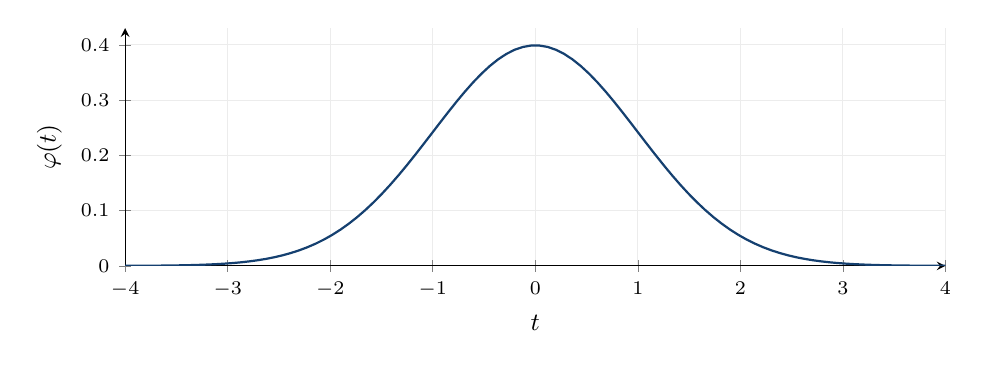
\begin{tikzpicture}\begin{axis}[base,width=12cm,height=4.6cm,xmin=-4,xmax=4,ymin=0,ymax=.43,xlabel={$t$},ylabel={$\varphi(t)$}]
\addplot[azul,thick,domain=-4:4]{exp(-x^2/2)/sqrt(2*pi)};
\end{axis}\end{tikzpicture}
\caption{Densidad normal estándar obtenida por normalización.}
\end{figure}

\clearpage
\section{Distribución acumulada normal: simetría y derivadas de sus argumentos}\label{unidad63}
La acumulada se define por
\[
\Phi(t)=\int_{-\infty}^t\varphi(u)\dd u.
\]
El teorema fundamental del cálculo implica
\(\Phi'(t)=\varphi(t)\).
Por simetría de la densidad,
\[
1-\Phi(t)=\Phi(-t).
\]
Para probarlo, cambiar \(u\) por \(-v\)
en la integral de \(t\) a infinito
transforma sus límites en menos infinito y \(-t\).

Para un producto de regresores,
la regla de la cadena da
\[
\frac{\partial}{\partial\gamma_l}
\Phi\left(\sum_{h=1}^qz_{ih}\gamma_h\right)
=\varphi\left(\sum_hz_{ih}\gamma_h\right)z_{il}.
\]
La segunda derivada es
\[
-\left(\sum_hz_{ih}\gamma_h\right)
\varphi\left(\sum_hz_{ih}\gamma_h\right)
z_{il}z_{ir}.
\]
Los datos permanecen fijos.
Una derivada por coeficiente añade
la coordenada correspondiente del dato.

Para el argumento estandarizado
\((y_i-\sum_jx_{ij}\beta_j)/\sigma\),
las derivadas son
\[
-\frac{x_{il}}{\sigma}
\quad\text{respecto de }\beta_l,\qquad
-\frac{y_i-\sum_jx_{ij}\beta_j}{\sigma^2}
\quad\text{respecto de }\sigma.
\]
Estas dos reglas se usarán muchas veces
en Tobit y en la verosimilitud de Heckman.

\begin{ejemplo}[Probabilidad de selección]
Si la suma \(\sum_lz_{il}\gamma_l\)
vale uno, la selección probit tiene
probabilidad \(\Phi(1)\approx.84134475\).
Su derivada respecto del intercepto
es \(\varphi(1)\approx.24197072\).
\end{ejemplo}
La acumulada no se reemplaza por
la densidad: una representa una
probabilidad y la otra su cambio
por unidad del argumento.

En los extremos, la probabilidad
puede acercarse a cero o uno,
mientras la densidad se vuelve pequeña.
Los cocientes de ambas pueden
permanecer grandes y exigir
evaluación numérica estable.

\clearpage
\section{Normal bivariada: construir la matriz de covarianza de dos errores}\label{unidad64}
Heckman utilizará un error de resultado
\(\varepsilon_i\) y otro de selección \(\nu_i\).
Condicionados en los regresores, supongamos
\[
\begin{pmatrix}\varepsilon_i\\\nu_i\end{pmatrix}
\sim\mathcal N_2\left[
\begin{pmatrix}0\\0\end{pmatrix},
\begin{pmatrix}\sigma^2&\rho\sigma\\\rho\sigma&1\end{pmatrix}
\right],
\quad \sigma>0,\ |\rho|<1.
\]
La varianza del segundo error se fija en uno
para identificar la escala de la ecuación binaria.
La covarianza es \(\rho\sigma\),
no \(\rho\sigma^2\).

El determinante de la matriz es
\(\sigma^2(1-\rho^2)>0\).
Su inversa por cofactores es
\[
\frac1{1-\rho^2}
\begin{pmatrix}
1/\sigma^2&-\rho/\sigma\\
-\rho/\sigma&1
\end{pmatrix}.
\]
La densidad conjunta es
\[
\frac{\exp\left\{
-\frac1{2(1-\rho^2)}
\left[\frac{e^2}{\sigma^2}
-\frac{2\rho ev}{\sigma}+v^2\right]\right\}}
{2\pi\sigma\sqrt{1-\rho^2}}.
\]
El término cruzado determina cómo
se inclinan sus curvas de densidad.

Una construcción equivalente usa
dos normales estándar independientes:
\[
\nu_i\sim\mathcal N(0,1),\quad u_i\sim\mathcal N(0,1),
\qquad
\varepsilon_i=\rho\sigma\nu_i
+\sigma\sqrt{1-\rho^2}\,u_i.
\]
Linealidad de esperanza da media cero.
La varianza es
\(\rho^2\sigma^2+\sigma^2(1-\rho^2)=\sigma^2\).
La covarianza con \(\nu_i\) es \(\rho\sigma\).

Esta construcción permite ver la parte
del error de resultado que comparte
el error de selección y la parte independiente.
Condicionar en un evento de \(\nu_i\)
altera la primera y deja intacta
la distribución de la segunda.

En \(|\rho|=1\), el determinante se anula
y la distribución pierde una dimensión.
Las fórmulas de densidad interior
no se aplican allí por simple sustitución.

\clearpage
\section{Completar cuadrados: derivar ambas normales condicionales}\label{unidad65}
En la densidad bivariada, completar
el cuadrado en el error de resultado da
\[
\frac{e^2}{\sigma^2}
-\frac{2\rho ev}{\sigma}+v^2
=\left(\frac e\sigma-\rho v\right)^2
+(1-\rho^2)v^2.
\]
Dividir por \(1-\rho^2\) separa
una densidad estándar en \(v\)
y una normal en \(e\) con media
\(\rho\sigma v\) y varianza
\(\sigma^2(1-\rho^2)\).
Por ello,
\[
\varepsilon_i\mid\nu_i=v
\sim\mathcal N(\rho\sigma v,\sigma^2(1-\rho^2)).
\]

Completar el cuadrado en el otro orden produce
\[
\frac{e^2}{\sigma^2}
-\frac{2\rho ev}{\sigma}+v^2
=(v-\rho e/\sigma)^2
+(1-\rho^2)e^2/\sigma^2.
\]
Así,
\[
\nu_i\mid\varepsilon_i=e
\sim\mathcal N(\rho e/\sigma,1-\rho^2).
\]
Se usarán las dos direcciones:
la primera para medias seleccionadas,
la segunda para la densidad conjunta
de resultado observado y selección.

\begin{ejemplo}[Correlación .5 y escala dos]
Condicionado en \(\nu_i=1\),
el error de resultado tiene media uno
y varianza tres.
Condicionado en \(\varepsilon_i=2\),
el error de selección tiene media .5
y varianza .75.
\end{ejemplo}
La correlación determina ambas medias,
pero las escalas de los errores
hacen distintos sus coeficientes.
No se intercambia \(\rho\sigma\)
con \(\rho/\sigma\).

Si \(\rho=0\), la densidad conjunta
factoriza en las dos marginales normales,
y los errores son independientes.
Para distribuciones no normales,
covarianza cero por sí sola
no garantiza esa independencia.

La distribución condicional aquí se
dedujo de una hipótesis bivariada específica.
No es una identidad válida para
cualquier pareja de errores
con la misma matriz de covarianza.

\clearpage
\section{Truncar una normal: obtener la densidad condicional}\label{unidad66}
Sea \(\nu_i\sim\mathcal N(0,1)\).
Condicionar en \(\nu_i>a\) restringe
los valores posibles, pero debe
mantener área total uno:
\[
f(v\mid\nu_i>a)
=\frac{\varphi(v)}{1-\Phi(a)}\mathbf1\{v>a\}.
\]
El denominador es la probabilidad
del evento condicionado.
Integrar la densidad restringida
produce exactamente uno.

En selección probit,
\[
S_i=1\left\{\sum_lz_{il}\gamma_l+\nu_i>0\right\}.
\]
Manteniendo fijos los regresores,
el evento es
\(\nu_i>-\sum_lz_{il}\gamma_l\).
Su probabilidad es
\[
1-\Phi\left(-\sum_lz_{il}\gamma_l\right)
=\Phi\left(\sum_lz_{il}\gamma_l\right).
\]
Por tanto la densidad seleccionada es
\[
\frac{\varphi(v)}
{\Phi(\sum_lz_{il}\gamma_l)}
\mathbf1\left\{v>-\sum_lz_{il}\gamma_l\right\}.
\]

El soporte cambia con los regresores.
Una baja probabilidad de selección
conserva solamente valores altos
del error \(\nu_i\).
Aunque su distribución original
tenga media cero, su media
entre seleccionados puede ser grande.

\begin{ejemplo}[Selección con intercepto cero]
El evento es \(\nu_i>0\),
y su densidad es \(2\varphi(v)\)
para valores positivos.
Su media no es cero:
el lado negativo se ha eliminado.
\end{ejemplo}
Censurar en cero conserva también
una masa para los valores eliminados.
Truncar y condicionar renormaliza
la densidad de los restantes.
Este cociente será central para
derivar Mills por integración.

No se puede convertir una distribución
seleccionada en una normal ordinaria
cambiando únicamente su media:
su forma y su varianza
también cambian con el truncamiento.

\clearpage
\section{Primer momento truncado: la integral que produce Mills}\label{unidad67}
La media de una normal estándar
condicionada en \(\nu_i>a\) es
\[
\frac{\int_a^\infty v\varphi(v)\dd v}
{1-\Phi(a)}.
\]
Usar \(\varphi'(v)=-v\varphi(v)\)
resuelve el numerador:
\[
\int_a^\infty v\varphi(v)\dd v
=-[\varphi(v)]_a^\infty=\varphi(a).
\]
La densidad tiende a cero en infinito.
La media truncada queda
\[
\E[\nu_i\mid\nu_i>a]
=\frac{\varphi(a)}{1-\Phi(a)}.
\]

Para el evento de selección,
el umbral es \(a=-\sum_lz_{il}\gamma_l\).
La simetría de densidad y acumulada produce
\[
\boxed{
\E[\nu_i\mid z_i,S_i=1]
=\frac{\varphi(\sum_lz_{il}\gamma_l)}
{\Phi(\sum_lz_{il}\gamma_l)}}.
\]
Esta es la razón inversa de Mills
que entra en Heckman.
Su signo es positivo para cualquier
argumento finito.

No es la probabilidad de selección.
En un argumento cero,
la probabilidad es \(1/2\),
pero el cociente es
\[
\frac{1/\sqrt{2\pi}}{1/2}
=\sqrt{2/\pi}\approx.79788456.
\]
Un cociente mayor que uno
no representa una probabilidad inválida:
representa una media condicional de un error.

\begin{ejemplo}[Evento raro]
Si el producto de selección vale \(-2\),
solo se seleccionan errores mayores que dos.
Su media tiene que superar dos.
La razón es aproximadamente \(2.37321553\),
coherente con ese soporte.
\end{ejemplo}
La nueva columna de segunda etapa
resume una media de error derivada
del mecanismo de selección y
de la hipótesis normal.
Su coeficiente en la ecuación
de resultado dependerá de la
covarianza entre ambos errores.

El nombre de la razón no reemplaza
la demostración: apareció al dividir
una integral de primer momento
por la probabilidad del evento.

\clearpage
\section{Segundo momento truncado: integración por partes completa}\label{unidad68}
El segundo momento condicionado es
\[
\E[\nu_i^2\mid\nu_i>a]
=\frac{\int_a^\infty v^2\varphi(v)\dd v}
{1-\Phi(a)}.
\]
Usando la derivada de la densidad,
\[
\begin{aligned}
\int_a^\infty v^2\varphi(v)\dd v
&=-\int_a^\infty v\varphi'(v)\dd v\\
&=-[v\varphi(v)]_a^\infty
+\int_a^\infty\varphi(v)\dd v\\
&=a\varphi(a)+1-\Phi(a).
\end{aligned}
\]
El término \(v\varphi(v)\) se anula
en infinito.
Al dividir queda
\[
\E[\nu_i^2\mid\nu_i>a]
=1+a\frac{\varphi(a)}{1-\Phi(a)}.
\]

En selección, sustituir el umbral
\(a=-\sum_lz_{il}\gamma_l\) produce
\[
\E[\nu_i^2\mid z_i,S_i=1]
=1-\left(\sum_lz_{il}\gamma_l\right)
\frac{\varphi(\sum_lz_{il}\gamma_l)}
{\Phi(\sum_lz_{il}\gamma_l)}.
\]
La varianza resta el cuadrado
de la media ya deducida:
\[
\boxed{
1-\frac{\varphi(\sum_lz_{il}\gamma_l)}
{\Phi(\sum_lz_{il}\gamma_l)}
\left[
\sum_lz_{il}\gamma_l
+\frac{\varphi(\sum_lz_{il}\gamma_l)}
{\Phi(\sum_lz_{il}\gamma_l)}
\right]}.
\]
El segundo momento y la varianza
no son la misma cantidad.

\begin{ejemplo}[Seminormal]
En producto de selección cero,
el segundo momento es uno
y la varianza es \(1-2/\pi\approx.36338023\).
La media positiva explica la diferencia.
\end{ejemplo}
Seleccionar errores de una sola cola
reduce su variación alrededor de
la nueva media bajo este modelo.
No necesariamente reduce el segundo
momento respecto de cero.

La misma expresión dará
heterocedasticidad en la ecuación
de resultado seleccionado.
Sus valores cambiarán entre filas
porque cambia el producto de selección.

\clearpage
\section{Momentos truncados de orden superior: deducir una recurrencia}\label{unidad69}
Para un entero \(m\ge2\),
usar \(v\varphi(v)=-\varphi'(v)\)
da la identidad
\[
\begin{aligned}
\int_a^\infty v^m\varphi(v)\dd v
&=-\int_a^\infty v^{m-1}\varphi'(v)\dd v\\
&=a^{m-1}\varphi(a)
+(m-1)\int_a^\infty v^{m-2}\varphi(v)\dd v.
\end{aligned}
\]
La integral de orden \(m\) se reduce
a otra de orden \(m-2\).
La frontera en infinito desaparece
porque cualquier potencia fija
por la densidad normal tiende a cero.

Las dos bases son
\[
\int_a^\infty\varphi(v)\dd v=1-\Phi(a),
\qquad
\int_a^\infty v\varphi(v)\dd v=\varphi(a).
\]
Por ejemplo,
\[
\int_a^\infty v^3\varphi(v)\dd v
=(a^2+2)\varphi(a),
\]
\[
\int_a^\infty v^4\varphi(v)\dd v
=(a^3+3a)\varphi(a)+3[1-\Phi(a)].
\]
Dividir por la probabilidad de truncamiento
convierte estos numeradores en
momentos condicionados.

Los momentos de tercero y cuarto orden
permiten estudiar asimetría y colas
de las distribuciones seleccionadas.
También aparecen al verificar
información esperada de una escala normal.

\begin{ejemplo}[Umbral cero]
El tercer momento seminormal es
\(2\sqrt{2/\pi}\approx1.59576912\),
y el cuarto es tres.
La asimetría es compatible con
un segundo momento igual al normal original.
\end{ejemplo}
Un modelo seleccionado no queda
completamente descrito por su media
y varianza. La distribución conserva
una forma truncada y puede ser
marcadamente asimétrica.

La recurrencia evita memorizar
cada integral por separado.
Se obtuvieron todos sus términos
mediante una misma integración por partes.

\clearpage
\section{Derivar Mills: cociente, densidad y acumulada}\label{unidad70}
Consideremos la función escalar
\(\varphi(t)/\Phi(t)\).
El cociente tiene denominador positivo
para todo \(t\) finito.
La regla de derivación produce
\[
\begin{aligned}
\frac{\dd}{\dd t}\frac{\varphi(t)}{\Phi(t)}
&=\frac{\varphi'(t)\Phi(t)-\varphi(t)\Phi'(t)}{\Phi(t)^2}\\
&=\frac{-t\varphi(t)\Phi(t)-\varphi(t)^2}{\Phi(t)^2}\\
&=-\frac{\varphi(t)}{\Phi(t)}
\left[t+\frac{\varphi(t)}{\Phi(t)}\right].
\end{aligned}
\]
Se utilizaron ambas derivadas,
no solamente la de la densidad.

Al aplicar esta función a datos,
\[
\begin{aligned}
&\frac{\partial}{\partial\gamma_l}
\frac{\varphi(\sum_hz_{ih}\gamma_h)}
{\Phi(\sum_hz_{ih}\gamma_h)}\\
&=-\frac{\varphi(\sum_hz_{ih}\gamma_h)}
{\Phi(\sum_hz_{ih}\gamma_h)}
\left[
\sum_hz_{ih}\gamma_h+
\frac{\varphi(\sum_hz_{ih}\gamma_h)}
{\Phi(\sum_hz_{ih}\gamma_h)}
\right]z_{il}.
\end{aligned}
\]
Cada fila conserva sus propios datos.
La coordenada \(z_{il}\) entra
por la regla de la cadena.

La derivada del logaritmo de la acumulada
es la razón misma:
\[
\frac{\dd}{\dd t}\log\Phi(t)=\frac{\varphi(t)}{\Phi(t)}.
\]
Por ello la derivada de Mills
es la segunda derivada de \(\log\Phi\).
Esta conexión determina
la curvatura de probit y Tobit.

\begin{ejemplo}[Centro]
En \(t=0\), la derivada es \(-2/\pi\).
Un pequeño aumento del argumento
disminuye la media del error seleccionado:
la selección se vuelve menos exigente.
\end{ejemplo}
La derivada no es constante.
Usar siempre el valor del centro
en un probit o en una corrección de selección
reemplazaría la función por
una aproximación local que
puede ser mala en las colas.

\clearpage
\section{Signo de Mills y cota de su derivada mediante una varianza}\label{unidad71}
La razón \(\varphi(t)/\Phi(t)\) es positiva.
Además,
\[
t+\frac{\varphi(t)}{\Phi(t)}>0.
\]
Para \(t\ge0\), esto es inmediato.
Para \(t<0\), la razón es
la media de una normal condicionada
a superar \(-t>0\).
Como todos sus valores superan
ese umbral, su media también lo supera.

La derivada deducida es entonces negativa:
\[
\frac{\dd}{\dd t}\frac{\varphi(t)}{\Phi(t)}<0.
\]
La varianza truncada satisface
\[
\Var(\nu_i\mid\nu_i>-t)
=1+\frac{\dd}{\dd t}\frac{\varphi(t)}{\Phi(t)}.
\]
Es estrictamente positiva para
un argumento finito, pues la
distribución no es degenerada.
Por tanto,
\[
-1<
\frac{\dd}{\dd t}\frac{\varphi(t)}{\Phi(t)}
<0.
\]
Esta cota no se obtuvo observando
un gráfico, sino conectando
la derivada con una varianza.

La positividad de la varianza
también implica que
\[
0<
\frac{\varphi(t)}{\Phi(t)}
\left[t+\frac{\varphi(t)}{\Phi(t)}\right]
<1.
\]
El factor será utilizado
para reducir la varianza del
error de resultado seleccionado.

\begin{ejemplo}[Interpretación de la pendiente]
Al incrementar el producto de selección,
la media del error truncado baja.
Su pendiente nunca es menor que \(-1\)
bajo la distribución normal.
\end{ejemplo}
Las cotas ayudan a comprobar
signos de Hessianas y a detectar
errores de implementación.
Un valor de varianza negativo
en una cola puede indicar
cancelación o redondeo numérico,
y no una propiedad real del modelo.

La cota pertenece a esta
razón normal específica.
No se transporta a cualquier
función de corrección de selección
sin deducir sus propios momentos.

\clearpage
\section{Segunda derivada de Mills: abrir producto y cadena}\label{unidad72}
Derivemos otra vez la identidad
\[
-\frac{\varphi(t)}{\Phi(t)}
\left[t+\frac{\varphi(t)}{\Phi(t)}\right].
\]
La regla del producto da
\[
\begin{aligned}
&-\left(\frac{\varphi(t)}{\Phi(t)}\right)'
\left[t+\frac{\varphi(t)}{\Phi(t)}\right]\\
&-\frac{\varphi(t)}{\Phi(t)}
\left[1+\left(\frac{\varphi(t)}{\Phi(t)}\right)'\right].
\end{aligned}
\]
Sustituir la primera derivada
y reunir términos produce
\[
\boxed{
\frac{\dd^2}{\dd t^2}\frac{\varphi(t)}{\Phi(t)}
=\frac{\varphi(t)}{\Phi(t)}
\left[
\left(t+\frac{\varphi(t)}{\Phi(t)}\right)
\left(t+2\frac{\varphi(t)}{\Phi(t)}\right)-1
\right]}.
\]
Cada producto es escalar.
Al usar un argumento lineal en \(\gamma\),
la segunda derivada cruzada multiplica
esta expresión por \(z_{il}z_{ir}\).

Esta fórmula permite calcular
cómo cambia el Jacobiano de
una segunda etapa al mover
parámetros de primera etapa.
También controla restos de Taylor
en una vecindad finita.

\begin{ejemplo}[Evaluación en cero]
Con \(\varphi(0)/\Phi(0)=\sqrt{2/\pi}\),
la segunda derivada es
\[
\sqrt{2/\pi}\left(\frac4\pi-1\right)
\approx.21801361.
\]
La primera derivada en el mismo punto
es aproximadamente \(-.63661977\).
\end{ejemplo}
Las funciones y sus derivadas
deben evaluarse en el argumento
completo de cada fila.
Dos registros con probabilidades
parecidas pueden tener sensibilidades
distintas si sus coordenadas
\(z_{il}\) son distintas.

Para una función vectorial
de todas las razones,
el Jacobiano tiene una fila
por observación y una columna
por coeficiente de selección.
Ese tamaño debe conservarse
al propagar la covarianza de \(\widehat\gamma\).

\clearpage
\section{Mills en la cola: deducir cotas por integración por partes}\label{unidad73}
Para \(a>0\), la cola normal superior es
\(\int_a^\infty\varphi(v)\dd v\).
Como \(v/a\ge1\),
\[
1-\Phi(a)<\frac1a\int_a^\infty v\varphi(v)\dd v
=\frac{\varphi(a)}a.
\]
La desigualdad es estricta
porque la densidad tiene masa
en valores mayores que \(a\).

Integrar por partes de otra forma da
\[
1-\Phi(a)=\frac{\varphi(a)}a
-\int_a^\infty\frac{\varphi(v)}{v^2}\dd v.
\]
El último integral no supera
\([1-\Phi(a)]/a^2\).
Reunir términos implica
\[
1-\Phi(a)>
\frac{a}{a^2+1}\varphi(a).
\]
Al invertir las dos cotas positivas,
\[
\boxed{
a<\frac{\varphi(a)}{1-\Phi(a)}<a+\frac1a}.
\]
Para el argumento \(t=-a\),
la razón de Mills de selección
queda acotada por esas cantidades.

La relación explica por qué
el cociente es grande cuando
la probabilidad de selección
es muy pequeña: solo sobreviven
errores en una cola alta.
No significa que la densidad
por sí sola sea grande.

\begin{ejemplo}[Argumento menos cinco]
Las cotas son cinco y 5.2.
La razón real es aproximadamente 5.18650397.
Ambos factores originales,
densidad y acumulada inferior,
son pequeños, pero su cociente
no lo es.
\end{ejemplo}
Las cotas permiten validar
un cálculo de cola sin
reproducir toda la integral.
Si una rutina devuelve cero
para esa razón, ha perdido
información por subdesbordamiento.

Para varianzas truncadas extremas,
restar cantidades casi iguales
puede requerir métodos de evaluación
más precisos que la fórmula directa.

\clearpage
\section{Evaluación estable de Mills y probabilidades extremas}\label{unidad74}
La expresión directa
\(\varphi(t)/\Phi(t)\) puede perder precisión
si ambos factores son muy pequeños.
Una forma estable trabaja con logaritmos:
\[
\frac{\varphi(t)}{\Phi(t)}
=\exp\left[-\frac{t^2}{2}
-\frac12\log(2\pi)-\log\Phi(t)\right].
\]
El valor \(\log\Phi(t)\) debe
evaluarse con un método de cola,
y no tomando el logaritmo
de un cero redondeado previamente.

Para probabilidades del complemento,
la identidad \(1-\Phi(t)=\Phi(-t)\)
evita restar de uno una
acumulada extremadamente próxima a uno.
La misma regla se aplica
en la log-verosimilitud de
selección no observada.

En una cola con \(t\ll0\),
la razón se aproxima a \(-t\),
con correcciones pequeñas.
La varianza truncada contiene
la diferencia entre uno
y un producto próximo a uno.
Esa cancelación puede perder
dígitos en cálculo ordinario.

\begin{ejemplo}[Una selección extremadamente rara]
Con \(t=-8\),
\(\Phi(t)\approx6.22096\cdot10^{-16}\).
Mills es aproximadamente 8.12136811,
y la varianza truncada aproximadamente .01432488.
Estos números son positivos y
coherentes con las cotas de cola.
\end{ejemplo}
La fórmula matemática sigue válida
en toda la recta real finita.
Una dificultad de aritmética
no modifica el modelo:
requiere una evaluación mejor
de la misma función.

En los laboratorios se calcularán
las razones con la forma logarítmica,
y se verificarán sus momentos
contra integración numérica
cuando la cola lo permita.

Redondear una probabilidad en
una tabla a cero no significa
que su probabilidad matemática
sea cero. La distinción es
especialmente relevante al calcular
derivadas y verosimilitudes.

\clearpage
\section{Seminormal: resolver sus momentos y su asimetría}\label{unidad75}
La normal condicionada en ser positiva
tiene densidad \(2\varphi(v)\)
para \(v>0\).
Sus dos primeros momentos son
\[
\E[\nu_i\mid\nu_i>0]=\sqrt{2/\pi},
\qquad
\E[\nu_i^2\mid\nu_i>0]=1.
\]
Su varianza es
\(1-2/\pi\).
La recurrencia de momentos da
tercer momento \(2\sqrt{2/\pi}\)
y cuarto momento tres.

Para calcular el tercer momento central,
abrir el cubo produce
\[
\begin{aligned}
&\E[(\nu_i-\sqrt{2/\pi})^3\mid\nu_i>0]\\
&=2\sqrt{2/\pi}
-3\sqrt{2/\pi}
+3(2/\pi)\sqrt{2/\pi}
-(2/\pi)^{3/2}\\
&=\sqrt{2/\pi}\left(\frac4\pi-1\right).
\end{aligned}
\]
Dividir por \((1-2/\pi)^{3/2}\)
da su coeficiente de asimetría.

La distribución tiene soporte positivo,
pero una cola derecha infinita.
Una normal ordinaria con la misma
media y varianza tendría soporte
en toda la recta.
Igualar momentos no iguala
las distribuciones.

\begin{ejemplo}[Error de selección con índice cero]
La selección toma exactamente
la mitad superior del error.
Su media .79788456
y varianza .36338023
se obtienen sin estimación alguna
si el parámetro de selección es conocido.
\end{ejemplo}
En Heckman, el error de resultado
es la suma de una parte
proporcional a este error truncado
y otra normal independiente.
Si la correlación no es cero,
su distribución seleccionada
también puede ser asimétrica.

La segunda etapa utiliza correctamente
su media y su varianza
bajo las hipótesis del modelo,
pero no presupone que la
distribución residual seleccionada
sea una normal homocedástica ordinaria.

\clearpage
\section{Truncamiento entre dos límites: normalizar y calcular dos momentos}\label{unidad76}
Si \(a<\nu_i<b\), la probabilidad del evento es
\(\Phi(b)-\Phi(a)>0\).
La densidad condicionada es
\[
\frac{\varphi(v)}{\Phi(b)-\Phi(a)}
\mathbf1\{a<v<b\}.
\]
La integral de primer momento
usa la misma derivada normal:
\[
\int_a^b v\varphi(v)\dd v
=\varphi(a)-\varphi(b).
\]
Por tanto,
\[
\E[\nu_i\mid a<\nu_i<b]
=\frac{\varphi(a)-\varphi(b)}
{\Phi(b)-\Phi(a)}.
\]
La integración por partes de orden dos produce
\[
\int_a^b v^2\varphi(v)\dd v
=a\varphi(a)-b\varphi(b)+\Phi(b)-\Phi(a).
\]
Al dividir y restar el cuadrado de la media,
\[
\begin{aligned}
\Var(\nu_i\mid a<\nu_i<b)
={}&1+\frac{a\varphi(a)-b\varphi(b)}
{\Phi(b)-\Phi(a)}\\
&-\left[\frac{\varphi(a)-\varphi(b)}
{\Phi(b)-\Phi(a)}\right]^2.
\end{aligned}
\]
Los dos términos de frontera importan.
Eliminar uno convertiría el evento
en una truncación de una sola cola.

\begin{ejemplo}[Intervalo simétrico]
Con \(a=-1,b=1\), la media es cero
porque las densidades de frontera
son iguales. La varianza es
\[
1-\frac{2\varphi(1)}{\Phi(1)-\Phi(-1)}
\approx.29112509.
\]
\end{ejemplo}
Estas fórmulas se usan en modelos
con límites inferiores y superiores,
y en datos que llegan solo
dentro de una ventana de valores.

Una censura de dos lados
conserva masas en los límites.
La distribución de los registros
interiores condicionados sí tiene
el denominador de esta unidad.
La verosimilitud del conjunto censurado
no lo agrega automáticamente
a cada observación interior.

\clearpage
\section{Probit: derivar gradiente y Hessiana con la razón normal completa}\label{unidad77}
Con \(S_i\) observado en todas las filas,
la probabilidad de selección es
\(\Phi(\sum_lz_{il}\gamma_l)\).
Su log-verosimilitud es
\[
\sum_i\left[
S_i\log\Phi(\sum_lz_{il}\gamma_l)
+(1-S_i)\log\Phi(-\sum_lz_{il}\gamma_l)\right].
\]
Derivar respecto de \(\gamma_r\) da
\[
\sum_i z_{ir}\left[
S_i\frac{\varphi(\sum_lz_{il}\gamma_l)}
{\Phi(\sum_lz_{il}\gamma_l)}
-(1-S_i)\frac{\varphi(-\sum_lz_{il}\gamma_l)}
{\Phi(-\sum_lz_{il}\gamma_l)}
\right].
\]
El signo negativo del segundo término
proviene de su argumento negativo.
La densidad es simétrica,
pero sus dos acumuladas no son iguales.

La segunda derivada entre coordenadas \(r,h\)
es la suma de \(z_{ir}z_{ih}\)
por la derivada de Mills
en el argumento correspondiente.
Ambos signos de cadena se multiplican,
por lo que el término no seleccionado
también tiene curvatura negativa.

Con la derivada de Mills entre \(-1,0\),
la Hessiana es semidefinida negativa.
Con rango completo y parámetros finitos,
es definida negativa.
La concavidad no garantiza por sí sola
existencia de un máximo finito
si los datos separan selección.

\begin{ejemplo}[Inicio cero]
En \(\gamma=0\), cada probabilidad es \(1/2\).
El gradiente es
\[
\sqrt{2/\pi}\sum_i z_i(2S_i-1),
\]
y el negativo de la Hessiana es
\[
\frac2\pi\sum_i z_iz_i\T.
\]
\end{ejemplo}
La primera etapa de Heckman utilizará
este objetivo sobre seleccionados
y no seleccionados juntos.
Excluir estos últimos antes del probit
impediría estimar el mecanismo
de selección de la población observada.

\clearpage
\section{Problema resuelto de Mills: producto de selección -3}\label{unidad78}
Una fila tiene \(z_i=(1,0)\T\)
y coeficientes de selección
\[
\gamma=\begin{pmatrix}-3.0000000\\0.5000000\end{pmatrix}.
\]

El producto completo es
\[
(1)(-3)+(0)(.5)=-3.
\]

El evento de selección exige un error estándar
por encima del negativo de ese resultado.
La probabilidad y densidad evaluadas son
\[
\Phi(-3)\approx0.001349898032,\qquad\varphi(-3)\approx0.004431848412.
\]

La integral de primer momento, dividida
por la probabilidad, produce
\[
\E[\nu_i\mid S_i=1,z_i]
=\frac{\varphi(-3)}{\Phi(-3)}
\approx3.2830986549.
\]

La integración de segundo orden y
la resta del cuadrado de la media dan
\[
\begin{aligned}
\E[\nu_i^2\mid S_i=1,z_i]&=1-(-3)(3.2830986549)\\
&\approx10.8492959648,\\
\Var(\nu_i\mid S_i=1,z_i)&\approx10.8492959648-(3.2830986549)^2\\
&=0.0705591868.\end{aligned}
\]

Supongamos ahora un error de resultado con
\(\sigma=2,\rho=.6\).
La construcción bivariada implica
\(\varepsilon_i=1.2\nu_i+1.6u_i\),
con \(u_i\) estándar independiente.
Su media y varianza seleccionadas son
\[
\begin{aligned}
\E[\varepsilon_i\mid S_i=1,z_i]&\approx1.2(3.2830986549)
=3.9397183859,\\
\Var(\varepsilon_i\mid S_i=1,z_i)&\approx1.2^2(0.0705591868)+1.6^2\\
&=2.6616052290.\end{aligned}
\]

Con \(x_i=(1,2)\T,\beta=(1,.5)\T\),
la media latente sin selección es
\((1)(1)+(2)(.5)=2\).
Entre seleccionados aumenta en
la media de error recién calculada.
No se interpreta el aumento como
un cambio del coeficiente causal.


\begin{figure}[H]\centering
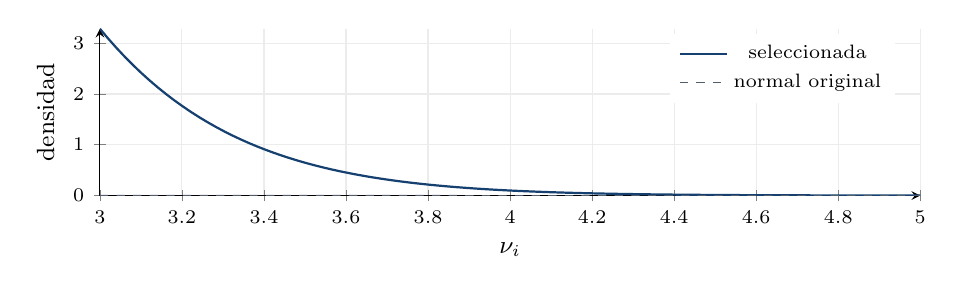
\begin{tikzpicture}\begin{axis}[base,width=12cm,height=3.7cm,xmin=3,xmax=5,xlabel={$\nu_i$},ylabel={densidad},legend pos=north east]
\addplot[azul,thick,domain=3:5]{exp(-x^2/2-(-6.607726221510)-ln(2*pi)/2)};\addplot[gris,dashed,domain=3:5]{exp(-x^2/2)/sqrt(2*pi)};\legend{seleccionada,normal original}
\end{axis}\end{tikzpicture}
\caption{Densidad del error de selección condicionado en la fila del problema.}
\end{figure}

La figura muestra una densidad condicionada,
sin una masa puntual en el límite.
Las cuentas emplean la hipótesis
normal bivariada explícita;
otra distribución de errores requeriría
recalcular las integrales de selección.

\clearpage
\section{Problema resuelto de Mills: producto de selección -1}\label{unidad79}
Una fila tiene \(z_i=(1,0)\T\)
y coeficientes de selección
\[
\gamma=\begin{pmatrix}-1.0000000\\0.5000000\end{pmatrix}.
\]

El producto completo es
\[
(1)(-1)+(0)(.5)=-1.
\]

El evento de selección exige un error estándar
por encima del negativo de ese resultado.
La probabilidad y densidad evaluadas son
\[
\Phi(-1)\approx0.1586552539,\qquad\varphi(-1)\approx0.2419707245.
\]

La integral de primer momento, dividida
por la probabilidad, produce
\[
\E[\nu_i\mid S_i=1,z_i]
=\frac{\varphi(-1)}{\Phi(-1)}
\approx1.5251352762.
\]

La integración de segundo orden y
la resta del cuadrado de la media dan
\[
\begin{aligned}
\E[\nu_i^2\mid S_i=1,z_i]&=1-(-1)(1.5251352762)\\
&\approx2.5251352762,\\
\Var(\nu_i\mid S_i=1,z_i)&\approx2.5251352762-(1.5251352762)^2\\
&=0.1990976656.\end{aligned}
\]

Supongamos ahora un error de resultado con
\(\sigma=2,\rho=.6\).
La construcción bivariada implica
\(\varepsilon_i=1.2\nu_i+1.6u_i\),
con \(u_i\) estándar independiente.
Su media y varianza seleccionadas son
\[
\begin{aligned}
\E[\varepsilon_i\mid S_i=1,z_i]&\approx1.2(1.5251352762)
=1.8301623314,\\
\Var(\varepsilon_i\mid S_i=1,z_i)&\approx1.2^2(0.1990976656)+1.6^2\\
&=2.8467006384.\end{aligned}
\]

Con \(x_i=(1,2)\T,\beta=(1,.5)\T\),
la media latente sin selección es
\((1)(1)+(2)(.5)=2\).
Entre seleccionados aumenta en
la media de error recién calculada.
No se interpreta el aumento como
un cambio del coeficiente causal.


\begin{figure}[H]\centering
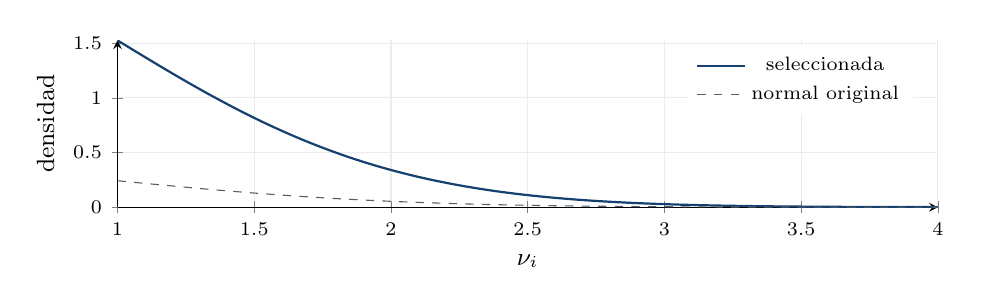
\begin{tikzpicture}\begin{axis}[base,width=12cm,height=3.7cm,xmin=1,xmax=4,xlabel={$\nu_i$},ylabel={densidad},legend pos=north east]
\addplot[azul,thick,domain=1:4]{exp(-x^2/2-(-1.841021645009)-ln(2*pi)/2)};\addplot[gris,dashed,domain=1:4]{exp(-x^2/2)/sqrt(2*pi)};\legend{seleccionada,normal original}
\end{axis}\end{tikzpicture}
\caption{Densidad del error de selección condicionado en la fila del problema.}
\end{figure}

La figura muestra una densidad condicionada,
sin una masa puntual en el límite.
Las cuentas emplean la hipótesis
normal bivariada explícita;
otra distribución de errores requeriría
recalcular las integrales de selección.

\clearpage
\section{Problema resuelto de Mills: producto de selección 0}\label{unidad80}
Una fila tiene \(z_i=(1,0)\T\)
y coeficientes de selección
\[
\gamma=\begin{pmatrix}0\\0.5000000\end{pmatrix}.
\]

El producto completo es
\[
(1)(0)+(0)(.5)=0.
\]

El evento de selección exige un error estándar
por encima del negativo de ese resultado.
La probabilidad y densidad evaluadas son
\[
\Phi(0)\approx0.5,\qquad\varphi(0)\approx0.3989422804.
\]

La integral de primer momento, dividida
por la probabilidad, produce
\[
\E[\nu_i\mid S_i=1,z_i]
=\frac{\varphi(0)}{\Phi(0)}
\approx0.7978845608.
\]

La integración de segundo orden y
la resta del cuadrado de la media dan
\[
\begin{aligned}
\E[\nu_i^2\mid S_i=1,z_i]&=1-(0)(0.7978845608)\\
&\approx1.0000000000,\\
\Var(\nu_i\mid S_i=1,z_i)&\approx1.0000000000-(0.7978845608)^2\\
&=0.3633802276.\end{aligned}
\]

Supongamos ahora un error de resultado con
\(\sigma=2,\rho=.6\).
La construcción bivariada implica
\(\varepsilon_i=1.2\nu_i+1.6u_i\),
con \(u_i\) estándar independiente.
Su media y varianza seleccionadas son
\[
\begin{aligned}
\E[\varepsilon_i\mid S_i=1,z_i]&\approx1.2(0.7978845608)
=0.9574614730,\\
\Var(\varepsilon_i\mid S_i=1,z_i)&\approx1.2^2(0.3633802276)+1.6^2\\
&=3.0832675278.\end{aligned}
\]

Con \(x_i=(1,2)\T,\beta=(1,.5)\T\),
la media latente sin selección es
\((1)(1)+(2)(.5)=2\).
Entre seleccionados aumenta en
la media de error recién calculada.
No se interpreta el aumento como
un cambio del coeficiente causal.


\begin{figure}[H]\centering
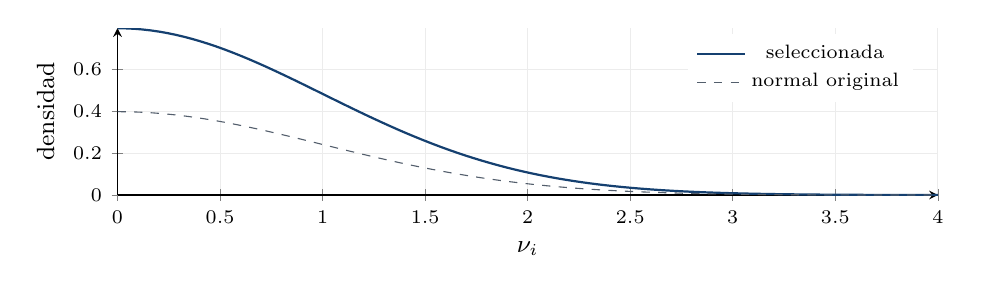
\begin{tikzpicture}\begin{axis}[base,width=12cm,height=3.7cm,xmin=-0,xmax=4,xlabel={$\nu_i$},ylabel={densidad},legend pos=north east]
\addplot[azul,thick,domain=-0:4]{exp(-x^2/2-(-0.693147180560)-ln(2*pi)/2)};\addplot[gris,dashed,domain=-0:4]{exp(-x^2/2)/sqrt(2*pi)};\legend{seleccionada,normal original}
\end{axis}\end{tikzpicture}
\caption{Densidad del error de selección condicionado en la fila del problema.}
\end{figure}

La figura muestra una densidad condicionada,
sin una masa puntual en el límite.
Las cuentas emplean la hipótesis
normal bivariada explícita;
otra distribución de errores requeriría
recalcular las integrales de selección.

\clearpage
\section{Problema resuelto de Mills: producto de selección 1}\label{unidad81}
Una fila tiene \(z_i=(1,0)\T\)
y coeficientes de selección
\[
\gamma=\begin{pmatrix}1.0000000\\0.5000000\end{pmatrix}.
\]

El producto completo es
\[
(1)(1)+(0)(.5)=1.
\]

El evento de selección exige un error estándar
por encima del negativo de ese resultado.
La probabilidad y densidad evaluadas son
\[
\Phi(1)\approx0.8413447461,\qquad\varphi(1)\approx0.2419707245.
\]

La integral de primer momento, dividida
por la probabilidad, produce
\[
\E[\nu_i\mid S_i=1,z_i]
=\frac{\varphi(1)}{\Phi(1)}
\approx0.2875999709.
\]

La integración de segundo orden y
la resta del cuadrado de la media dan
\[
\begin{aligned}
\E[\nu_i^2\mid S_i=1,z_i]&=1-(1)(0.2875999709)\\
&\approx0.7124000291,\\
\Var(\nu_i\mid S_i=1,z_i)&\approx0.7124000291-(0.2875999709)^2\\
&=0.6296862858.\end{aligned}
\]

Supongamos ahora un error de resultado con
\(\sigma=2,\rho=.6\).
La construcción bivariada implica
\(\varepsilon_i=1.2\nu_i+1.6u_i\),
con \(u_i\) estándar independiente.
Su media y varianza seleccionadas son
\[
\begin{aligned}
\E[\varepsilon_i\mid S_i=1,z_i]&\approx1.2(0.2875999709)
=0.3451199651,\\
\Var(\varepsilon_i\mid S_i=1,z_i)&\approx1.2^2(0.6296862858)+1.6^2\\
&=3.4667482515.\end{aligned}
\]

Con \(x_i=(1,2)\T,\beta=(1,.5)\T\),
la media latente sin selección es
\((1)(1)+(2)(.5)=2\).
Entre seleccionados aumenta en
la media de error recién calculada.
No se interpreta el aumento como
un cambio del coeficiente causal.


\begin{figure}[H]\centering
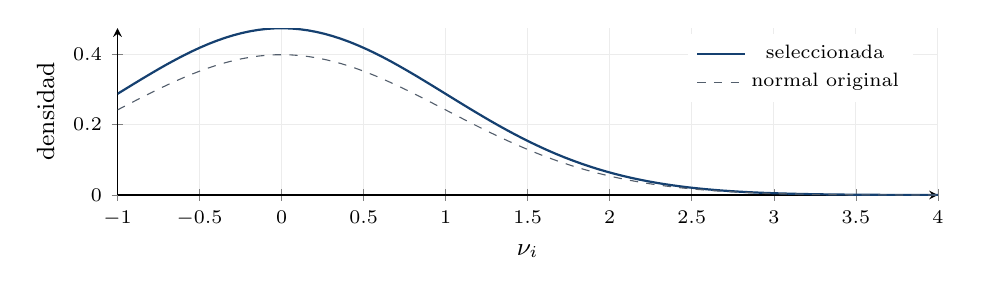
\begin{tikzpicture}\begin{axis}[base,width=12cm,height=3.7cm,xmin=-1,xmax=4,xlabel={$\nu_i$},ylabel={densidad},legend pos=north east]
\addplot[azul,thick,domain=-1:4]{exp(-x^2/2-(-0.172753779023)-ln(2*pi)/2)};\addplot[gris,dashed,domain=-1:4]{exp(-x^2/2)/sqrt(2*pi)};\legend{seleccionada,normal original}
\end{axis}\end{tikzpicture}
\caption{Densidad del error de selección condicionado en la fila del problema.}
\end{figure}

La figura muestra una densidad condicionada,
sin una masa puntual en el límite.
Las cuentas emplean la hipótesis
normal bivariada explícita;
otra distribución de errores requeriría
recalcular las integrales de selección.

\clearpage
\section{Problema resuelto de Mills: producto de selección 3}\label{unidad82}
Una fila tiene \(z_i=(1,0)\T\)
y coeficientes de selección
\[
\gamma=\begin{pmatrix}3.0000000\\0.5000000\end{pmatrix}.
\]

El producto completo es
\[
(1)(3)+(0)(.5)=3.
\]

El evento de selección exige un error estándar
por encima del negativo de ese resultado.
La probabilidad y densidad evaluadas son
\[
\Phi(3)\approx0.998650102,\qquad\varphi(3)\approx0.004431848412.
\]

La integral de primer momento, dividida
por la probabilidad, produce
\[
\E[\nu_i\mid S_i=1,z_i]
=\frac{\varphi(3)}{\Phi(3)}
\approx0.0044378390.
\]

La integración de segundo orden y
la resta del cuadrado de la media dan
\[
\begin{aligned}
\E[\nu_i^2\mid S_i=1,z_i]&=1-(3)(0.0044378390)\\
&\approx0.9866864829,\\
\Var(\nu_i\mid S_i=1,z_i)&\approx0.9866864829-(0.0044378390)^2\\
&=0.9866667885.\end{aligned}
\]

Supongamos ahora un error de resultado con
\(\sigma=2,\rho=.6\).
La construcción bivariada implica
\(\varepsilon_i=1.2\nu_i+1.6u_i\),
con \(u_i\) estándar independiente.
Su media y varianza seleccionadas son
\[
\begin{aligned}
\E[\varepsilon_i\mid S_i=1,z_i]&\approx1.2(0.0044378390)
=0.0053254069,\\
\Var(\varepsilon_i\mid S_i=1,z_i)&\approx1.2^2(0.9866667885)+1.6^2\\
&=3.9808001754.\end{aligned}
\]

Con \(x_i=(1,2)\T,\beta=(1,.5)\T\),
la media latente sin selección es
\((1)(1)+(2)(.5)=2\).
Entre seleccionados aumenta en
la media de error recién calculada.
No se interpreta el aumento como
un cambio del coeficiente causal.


\begin{figure}[H]\centering
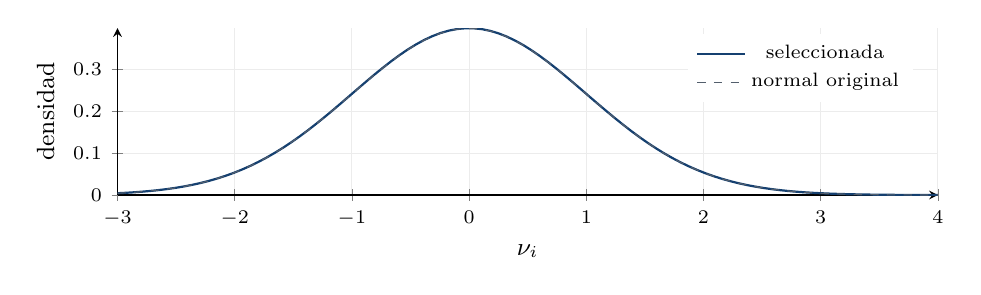
\begin{tikzpicture}\begin{axis}[base,width=12cm,height=3.7cm,xmin=-3,xmax=4,xlabel={$\nu_i$},ylabel={densidad},legend pos=north east]
\addplot[azul,thick,domain=-3:4]{exp(-x^2/2-(-0.001350809965)-ln(2*pi)/2)};\addplot[gris,dashed,domain=-3:4]{exp(-x^2/2)/sqrt(2*pi)};\legend{seleccionada,normal original}
\end{axis}\end{tikzpicture}
\caption{Densidad del error de selección condicionado en la fila del problema.}
\end{figure}

La figura muestra una densidad condicionada,
sin una masa puntual en el límite.
Las cuentas emplean la hipótesis
normal bivariada explícita;
otra distribución de errores requeriría
recalcular las integrales de selección.

\clearpage
\section{Problema resuelto de Mills: producto de selección -8}\label{unidad83}
Una fila tiene \(z_i=(1,0)\T\)
y coeficientes de selección
\[
\gamma=\begin{pmatrix}-8.0000000\\0.5000000\end{pmatrix}.
\]

El producto completo es
\[
(1)(-8)+(0)(.5)=-8.
\]

El evento de selección exige un error estándar
por encima del negativo de ese resultado.
La probabilidad y densidad evaluadas son
\[
\Phi(-8)\approx6.220960574e-16,\qquad\varphi(-8)\approx5.052271084e-15.
\]

La integral de primer momento, dividida
por la probabilidad, produce
\[
\E[\nu_i\mid S_i=1,z_i]
=\frac{\varphi(-8)}{\Phi(-8)}
\approx8.1213681122.
\]

La integración de segundo orden y
la resta del cuadrado de la media dan
\[
\begin{aligned}
\E[\nu_i^2\mid S_i=1,z_i]&=1-(-8)(8.1213681122)\\
&\approx65.9709448979,\\
\Var(\nu_i\mid S_i=1,z_i)&\approx65.9709448979-(8.1213681122)^2\\
&=0.0143248834.\end{aligned}
\]

Supongamos ahora un error de resultado con
\(\sigma=2,\rho=.6\).
La construcción bivariada implica
\(\varepsilon_i=1.2\nu_i+1.6u_i\),
con \(u_i\) estándar independiente.
Su media y varianza seleccionadas son
\[
\begin{aligned}
\E[\varepsilon_i\mid S_i=1,z_i]&\approx1.2(8.1213681122)
=9.7456417347,\\
\Var(\varepsilon_i\mid S_i=1,z_i)&\approx1.2^2(0.0143248834)+1.6^2\\
&=2.5806278322.\end{aligned}
\]

Con \(x_i=(1,2)\T,\beta=(1,.5)\T\),
la media latente sin selección es
\((1)(1)+(2)(.5)=2\).
Entre seleccionados aumenta en
la media de error recién calculada.
No se interpreta el aumento como
un cambio del coeficiente causal.


\begin{figure}[H]\centering
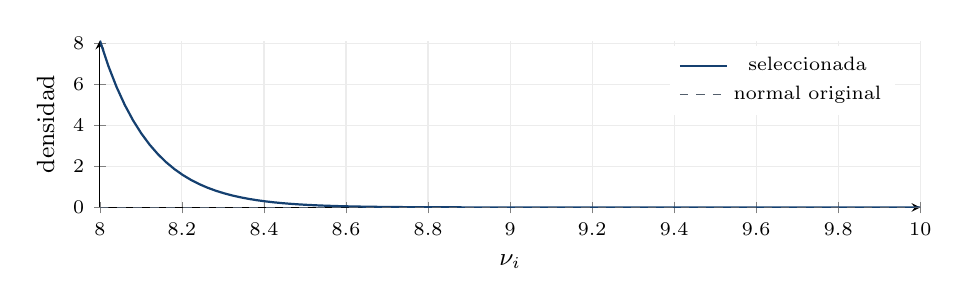
\begin{tikzpicture}\begin{axis}[base,width=12cm,height=3.7cm,xmin=8,xmax=10,xlabel={$\nu_i$},ylabel={densidad},legend pos=north east]
\addplot[azul,thick,domain=8:10]{exp(-x^2/2-(-35.013437159915)-ln(2*pi)/2)};\addplot[gris,dashed,domain=8:10]{exp(-x^2/2)/sqrt(2*pi)};\legend{seleccionada,normal original}
\end{axis}\end{tikzpicture}
\caption{Densidad del error de selección condicionado en la fila del problema.}
\end{figure}

La figura muestra una densidad condicionada,
sin una masa puntual en el límite.
Las cuentas emplean la hipótesis
normal bivariada explícita;
otra distribución de errores requeriría
recalcular las integrales de selección.

\clearpage
\addcontentsline{toc}{part}{Tobit: censura, momentos y máxima verosimilitud}
\pdfbookmark[0]{Tobit: censura, momentos y máxima verosimilitud}{parte84}
\section{Modelo Tobit: definir el latente y el observado antes de estimar}\label{unidad84}
El modelo latente es
\[
Y_i^\ast=\sum_{j=1}^k x_{ij}\beta_j+\varepsilon_i,
\qquad\varepsilon_i\mid x_i\sim\mathcal N(0,\sigma^2),
\quad \sigma>0.
\]
El observado está censurado inferiormente en cero:
\[
Y_i=\max(0,Y_i^\ast).
\]
Los valores negativos latentes no se observan
como negativos: todos generan el mismo cero.
Los positivos conservan su magnitud.

Manteniendo \(x_i\) fijo,
\[
\Prob(Y_i=0\mid x_i)
=\Phi\left(-\frac{\sum_jx_{ij}\beta_j}{\sigma}\right).
\]
Esto se deduce de
\(\varepsilon_i\le-\sum_jx_{ij}\beta_j\),
dividiendo ambos lados por la escala positiva.
La probabilidad positiva es
\[
\Prob(Y_i>0\mid x_i)
=\Phi\left(\frac{\sum_jx_{ij}\beta_j}{\sigma}\right).
\]
Las dos probabilidades suman uno
por simetría normal.

Para \(y_i>0\), la densidad observable es
\[
\frac1\sigma
\varphi\left(\frac{y_i-\sum_jx_{ij}\beta_j}{\sigma}\right).
\]
La masa del cero y el área positiva
forman la distribución mixta completa.
No se divide la densidad positiva
por la probabilidad de positividad
en esta distribución sin condicionar.

\begin{ejemplo}[Media latente uno y escala uno]
La probabilidad de censura es
\(\Phi(-1)\approx.15865525\).
La media observada no es exactamente uno:
la cola negativa se ha reemplazado
por el valor cero.
\end{ejemplo}
El modelo original de Tobin estudia
relaciones con respuestas limitadas \cite{tobin1958}.
La deducción de esta parte se basa
en el mecanismo normal de censura
que acabamos de especificar.

Un gran número de ceros puede proceder
de otros mecanismos, como una decisión
de participación separada.
La frecuencia de ceros por sí sola
no demuestra que Tobit sea
el modelo apropiado de una aplicación.

\clearpage
\section{Media observada Tobit: resolver el integral de positivos}\label{unidad85}
La masa del cero no aporta
al primer momento. La media es
\[
\E[Y_i\mid x_i]
=\int_0^\infty y\,\frac1\sigma
\varphi\left(\frac{y-\sum_jx_{ij}\beta_j}{\sigma}\right)\dd y.
\]
Hagamos el cambio
\(u=(y-\sum_jx_{ij}\beta_j)/\sigma\).
Entonces \(y=\sum_jx_{ij}\beta_j+\sigma u\),
\(\dd y=\sigma\dd u\),
y el límite inferior es
\(-\sum_jx_{ij}\beta_j/\sigma\).

Separar los dos términos produce
\[
\begin{aligned}
\E[Y_i\mid x_i]
={}&\left(\sum_jx_{ij}\beta_j\right)
\int_{-\sum_jx_{ij}\beta_j/\sigma}^\infty\varphi(u)\dd u\\
&+\sigma\int_{-\sum_jx_{ij}\beta_j/\sigma}^\infty u\varphi(u)\dd u.
\end{aligned}
\]
Las integrales ya se dedujeron:
la primera es \(\Phi(\sum_jx_{ij}\beta_j/\sigma)\);
la segunda es \(\varphi(\sum_jx_{ij}\beta_j/\sigma)\).
Así,
\[
\boxed{
\E[Y_i\mid x_i]
=\left(\sum_jx_{ij}\beta_j\right)
\Phi\left(\frac{\sum_jx_{ij}\beta_j}{\sigma}\right)
+\sigma\varphi\left(\frac{\sum_jx_{ij}\beta_j}{\sigma}\right)}.
\]
La suma lineal latente permanece visible
en ambas funciones.

\begin{ejemplo}[Latente centrado]
Si el producto es cero,
la media observada es \(\sigma/\sqrt{2\pi}\),
aunque la media latente sea cero.
Para \(\sigma=1\), vale aproximadamente .39894228.
\end{ejemplo}
Una media latente negativa no
implica una media observada negativa:
las respuestas observadas son no negativas.
El término de densidad y la
probabilidad positiva reflejan
esa transformación.

La pendiente de la media observada
no coincide en general con \(\beta_j\).
Se calculará derivando esta
expresión completa, para comprobar
qué términos se cancelan y
qué cantidad queda como efecto marginal.

\clearpage
\section{Segundo momento Tobit: abrir todos los términos del cuadrado}\label{unidad86}
La integración de \(Y_i^2\) usa
el mismo cambio de variable.
El cuadrado de
\(\sum_jx_{ij}\beta_j+\sigma u\)
genera tres términos:
\[
\begin{aligned}
&\left(\sum_jx_{ij}\beta_j\right)^2
+2\sigma\left(\sum_jx_{ij}\beta_j\right)u
+\sigma^2u^2.
\end{aligned}
\]
Cada uno se integra desde
\(-\sum_jx_{ij}\beta_j/\sigma\)
hasta infinito con densidad \(\varphi(u)\).

El integral de orden cero es
\(\Phi(\sum_jx_{ij}\beta_j/\sigma)\).
El de orden uno es la densidad
en ese argumento.
El de orden dos es
\[
\Phi\left(\frac{\sum_jx_{ij}\beta_j}{\sigma}\right)
-\frac{\sum_jx_{ij}\beta_j}{\sigma}
\varphi\left(\frac{\sum_jx_{ij}\beta_j}{\sigma}\right).
\]
Sustituir los tres y combinar
los dos términos de densidad da
\[
\begin{aligned}
\E[Y_i^2\mid x_i]
={}&\left[
\left(\sum_jx_{ij}\beta_j\right)^2+\sigma^2
\right]\Phi\left(\frac{\sum_jx_{ij}\beta_j}{\sigma}\right)\\
&+\sigma\left(\sum_jx_{ij}\beta_j\right)
\varphi\left(\frac{\sum_jx_{ij}\beta_j}{\sigma}\right).
\end{aligned}
\]
El cruce original tenía factor dos;
una parte se cancela con
el término de frontera de orden dos.
Omitir ese término impediría
obtener el coeficiente final correcto.

La varianza observada se calcula
restando el cuadrado de la
media completa de la unidad anterior.
No se resta el cuadrado
del producto lineal latente.

\begin{ejemplo}[Producto cero]
El segundo momento observado es
\(\sigma^2/2\).
La varianza es
\[
\sigma^2\left(\frac12-\frac1{2\pi}\right).
\]
Para escala uno vale .34084506,
distinta tanto de uno
como de la varianza seminormal.
\end{ejemplo}
La seminormal condiciona en positividad;
Tobit conserva una masa en cero.
Son distribuciones diferentes
con momentos diferentes.

\clearpage
\section{Varianza Tobit y por qué aparece heterocedasticidad observable}\label{unidad87}
Reunir primer y segundo momentos produce
\[
\begin{aligned}
\Var(Y_i\mid x_i)
={}&\left[
\left(\sum_jx_{ij}\beta_j\right)^2+\sigma^2
\right]\Phi\left(\frac{\sum_jx_{ij}\beta_j}{\sigma}\right)\\
&+\sigma\left(\sum_jx_{ij}\beta_j\right)
\varphi\left(\frac{\sum_jx_{ij}\beta_j}{\sigma}\right)\\
&-\left[
\left(\sum_jx_{ij}\beta_j\right)
\Phi\left(\frac{\sum_jx_{ij}\beta_j}{\sigma}\right)
+\sigma\varphi\left(\frac{\sum_jx_{ij}\beta_j}{\sigma}\right)
\right]^2.
\end{aligned}
\]
La expresión depende de los
regresores aunque el error latente
tenga escala constante.
La transformación de censura
genera una distribución observable
que cambia de forma y dispersión.

Cuando el producto lineal
es muy negativo respecto de la escala,
casi todas las respuestas son cero.
La varianza observada se acerca a cero.
Cuando es muy positivo,
la censura es poco frecuente
y la varianza se aproxima a \(\sigma^2\).

Estas propiedades no contradicen
la homocedasticidad latente:
la variable observada y
el error latente son objetos distintos.
No se toma una muestra de positivos
y se atribuye su varianza
directamente a \(\sigma^2\).

\begin{ejemplo}[Tres índices con escala uno]
Con productos \(-1,0,1\),
las medias observadas son aproximadamente
.08331547, .39894228 y 1.08331547.
Sus varianzas son diferentes
y se obtienen sustituyendo en
la misma fórmula de tres líneas.
\end{ejemplo}
La varianza de un coeficiente
estimado se estudiará con
la información del modelo,
no con esta varianza
de una respuesta individual.

Para respuestas independientes dado
el diseño, la covarianza observable
entre dos filas diferentes es cero.
Sus medias estimadas pueden
seguir correlacionadas por
compartir los mismos coeficientes.
La distinción se conserva
al construir intervalos y predicciones.

\clearpage
\section{Media de positivos: conectar Tobit con una normal truncada}\label{unidad88}
Condicionar en \(Y_i>0\)
es condicionar el latente en ser positivo.
La densidad se renormaliza por
\(\Phi(\sum_jx_{ij}\beta_j/\sigma)\).
El error estándar debe superar
\(-\sum_jx_{ij}\beta_j/\sigma\).
Por la media truncada deducida,
\[
\begin{aligned}
\E[Y_i\mid Y_i>0,x_i]
={}&\sum_jx_{ij}\beta_j\\
&+\sigma
\frac{\varphi(\sum_jx_{ij}\beta_j/\sigma)}
{\Phi(\sum_jx_{ij}\beta_j/\sigma)}.
\end{aligned}
\]
La razón de Mills aparece
con el argumento de la ecuación latente
dividido por la escala.

La varianza condicionada es
\[
\begin{aligned}
\sigma^2\Bigg\{1-&
\frac{\varphi(\sum_jx_{ij}\beta_j/\sigma)}
{\Phi(\sum_jx_{ij}\beta_j/\sigma)}\\
&\cdot\left[
\frac{\sum_jx_{ij}\beta_j}{\sigma}
+\frac{\varphi(\sum_jx_{ij}\beta_j/\sigma)}
{\Phi(\sum_jx_{ij}\beta_j/\sigma)}
\right]\Bigg\}.
\end{aligned}
\]
Esta varianza no incluye la
variación entre cero y positivo
porque ya se condicionó
en la parte positiva.

La ley de esperanza total comprueba
la relación entre ambas medias:
\[
\E[Y_i\mid x_i]
=\Prob(Y_i>0\mid x_i)
\,\E[Y_i\mid Y_i>0,x_i].
\]
Sustituir las expresiones cancela
la acumulada del cociente
y recupera la fórmula Tobit completa.

\begin{ejemplo}[Producto cero]
La media positiva es
\(\sigma\sqrt{2/\pi}\).
Multiplicarla por probabilidad \(1/2\)
da \(\sigma/\sqrt{2\pi}\),
la media sin condicionar.
\end{ejemplo}
La ecuación de una muestra
solo de positivos tendría
esa media no lineal,
y no el producto latente original.
MCO sobre los positivos no
recupera automáticamente
los coeficientes del latente.

\clearpage
\section{Efecto marginal Tobit en la media observada: cancelar los términos}\label{unidad89}
Derivemos la media observada respecto de \(\beta_l\).
El producto \(\sum_jx_{ij}\beta_j\) tiene derivada \(x_{il}\).
El argumento estandarizado tiene derivada \(x_{il}/\sigma\).
La regla del producto genera
\[
\begin{aligned}
\frac{\partial}{\partial\beta_l}\E[Y_i\mid x_i]
={}&x_{il}\Phi\left(\frac{\sum_jx_{ij}\beta_j}{\sigma}\right)\\
&+\left(\sum_jx_{ij}\beta_j\right)
\varphi\left(\frac{\sum_jx_{ij}\beta_j}{\sigma}\right)\frac{x_{il}}{\sigma}\\
&-\sigma\left(\frac{\sum_jx_{ij}\beta_j}{\sigma}\right)
\varphi\left(\frac{\sum_jx_{ij}\beta_j}{\sigma}\right)\frac{x_{il}}{\sigma}.
\end{aligned}
\]
Las últimas dos líneas son opuestas.
Por eso queda
\[
\frac{\partial}{\partial\beta_l}\E[Y_i\mid x_i]
=x_{il}\Phi\left(\frac{\sum_jx_{ij}\beta_j}{\sigma}\right).
\]
La derivada respecto del dato \(x_{il}\),
cuando puede variar continuamente y sin
cambiar otras columnas, es
\[
\beta_l\Phi\left(\frac{\sum_jx_{ij}\beta_j}{\sigma}\right).
\]
Una cambia el coeficiente,
la otra cambia el regresor.
Las dos no se confunden.

Si el dato es binario,
el efecto discreto se calcula
como diferencia de dos medias
completas, no como derivada
por una unidad arbitrariamente grande.
Las interacciones exigen cambiar
también las columnas que dependan
de ese dato.

\begin{ejemplo}[Pendiente .7]
Con producto estandarizado cero,
el efecto marginal observado es .35.
Con producto uno, es
\(.7\Phi(1)\approx.58894132\).
El coeficiente latente es el
mismo .7 en ambos individuos.
\end{ejemplo}
El efecto varía por fila
porque cambia la probabilidad
de respuesta positiva.
La media de efectos marginales
se calcula promediando las
derivadas de todas las filas,
y no evaluando necesariamente
una sola fila de datos promedio.

\clearpage
\section{Derivadas Tobit de probabilidad, positivos y escala}\label{unidad90}
La probabilidad de respuesta positiva es
\(\Phi(\sum_jx_{ij}\beta_j/\sigma)\).
Sus derivadas son
\[
\frac{\partial}{\partial\beta_l}\Prob(Y_i>0\mid x_i)
=\frac{x_{il}}{\sigma}
\varphi\left(\frac{\sum_jx_{ij}\beta_j}{\sigma}\right),
\]
\[
\frac{\partial}{\partial\sigma}\Prob(Y_i>0\mid x_i)
=-\frac{\sum_jx_{ij}\beta_j}{\sigma^2}
\varphi\left(\frac{\sum_jx_{ij}\beta_j}{\sigma}\right).
\]
Aumentar escala mueve la probabilidad
hacia un medio: el signo depende
de la media latente.

Para la media entre positivos,
la derivada respecto del coeficiente es
\[
\begin{aligned}
x_{il}\Bigg\{1-&
\frac{\varphi(\sum_jx_{ij}\beta_j/\sigma)}
{\Phi(\sum_jx_{ij}\beta_j/\sigma)}\\
&\cdot\left[
\frac{\sum_jx_{ij}\beta_j}{\sigma}
+\frac{\varphi(\sum_jx_{ij}\beta_j/\sigma)}
{\Phi(\sum_jx_{ij}\beta_j/\sigma)}
\right]\Bigg\}.
\end{aligned}
\]
El corchete es la varianza
estándar truncada.
La media positiva cambia más
lentamente que la media latente
respecto de su producto.

Derivar la media sin condicionar
respecto de escala genera
una cancelación análoga:
\[
\frac{\partial}{\partial\sigma}\E[Y_i\mid x_i]
=\varphi\left(\frac{\sum_jx_{ij}\beta_j}{\sigma}\right).
\]
Es positiva: con media latente fija,
más dispersión aumenta la media
de la parte positiva retenida.

\begin{ejemplo}[Centro]
Con producto cero, la probabilidad positiva
no cambia con la escala: sigue en \(1/2\).
La media positiva y la media observada
sí crecen proporcionalmente con ella.
\end{ejemplo}
El modelo combina una probabilidad
de pasar el límite y una magnitud
condicionada en pasarlo.
Las derivadas de ambos componentes
permiten distinguir el margen
extensivo del margen intensivo
sin atribuir toda la respuesta
al coeficiente latente.

\clearpage
\section{Derivar la varianza Tobit: primer y segundo momento juntos}\label{unidad91}
Sea el producto lineal el argumento
que cambia, manteniendo fija la escala.
Derivar el segundo momento observado
y abrir sus productos permite comprobar
\[
\frac{\partial}{\partial\beta_l}
\E[Y_i^2\mid x_i]=2x_{il}\E[Y_i\mid x_i].
\]
Los términos de densidad se cancelan
al combinar sus tres fuentes:
el cuadrado de la media,
la escala y el cruce.

La derivada del cuadrado de la
media es dos veces la media
por su derivada. Por tanto,
\[
\frac{\partial}{\partial\beta_l}\Var(Y_i\mid x_i)
=2x_{il}\E[Y_i\mid x_i]
\left[1-\Phi\left(\frac{\sum_jx_{ij}\beta_j}{\sigma}\right)\right].
\]
Respecto del producto latente,
la varianza aumenta porque
la media observada es positiva
y el complemento de probabilidad
es positivo en argumentos finitos.

Para escala, el segundo momento
tiene derivada
\[
\frac{\partial}{\partial\sigma}\E[Y_i^2\mid x_i]
=2\sigma\Phi\left(\frac{\sum_jx_{ij}\beta_j}{\sigma}\right).
\]
Restar la derivada del cuadrado
de la media produce
\[
\begin{aligned}
\frac{\partial}{\partial\sigma}\Var(Y_i\mid x_i)
={}&2\sigma\Phi\left(\frac{\sum_jx_{ij}\beta_j}{\sigma}\right)\\
&-2\E[Y_i\mid x_i]
\varphi\left(\frac{\sum_jx_{ij}\beta_j}{\sigma}\right).
\end{aligned}
\]
Estas identidades permiten
comprobar numéricamente las fórmulas
de momentos sin repetir
todas sus integrales.

\begin{ejemplo}[Centro y escala uno]
La derivada de varianza por producto
es .39894228.
La derivada por escala es
\(1-1/\pi\approx.68169011\).
Esta última coincide con derivar
\(\sigma^2(1/2-1/(2\pi))\)
en producto cero.
\end{ejemplo}
Una ecuación latente con varianza
constante no implica una
matriz de errores observables
con todas las diagonales iguales.
La censura afecta tanto
media como dispersión.

\clearpage
\section{Verosimilitud Tobit: multiplicar masas y densidades}\label{unidad92}
Las filas son independientes condicionado
en el diseño. Para cada cero,
la contribución es la masa censurada.
Para cada positivo, la densidad
del latente observado.
La verosimilitud completa es
\[
\begin{aligned}
&\prod_{y_i=0}
\Phi\left(-\frac{\sum_jx_{ij}\beta_j}{\sigma}\right)\\
&\quad\cdot\prod_{y_i>0}
\frac1\sigma
\varphi\left(\frac{y_i-\sum_jx_{ij}\beta_j}{\sigma}\right).
\end{aligned}
\]
Los dos productos recorren
conjuntos distintos de filas.

Tomar logaritmos produce
\[
\begin{aligned}
\ell(\beta,\sigma)
={}&\sum_{y_i=0}
\log\Phi\left(-\frac{\sum_jx_{ij}\beta_j}{\sigma}\right)\\
&+\sum_{y_i>0}\left[
-\log\sigma-\frac12\log(2\pi)
-\frac{(y_i-\sum_jx_{ij}\beta_j)^2}{2\sigma^2}
\right].
\end{aligned}
\]
El término \(-\log\sigma\)
proviene del Jacobiano de escala.
No se puede omitir si
la escala se estima.

La contribución positiva no incluye
un denominador \(\Phi\).
Ese denominador pertenece a una
muestra condicionada en positividad.
Agregarlo aquí cambiaría el
modelo censurado por uno truncado.

\begin{ejemplo}[Una fila de cada tipo]
Con producto latente cero y escala uno,
un cero aporta \(\log(1/2)\).
Un positivo de valor uno aporta
\(-\tfrac12\log(2\pi)-1/2\).
Las dos contribuciones tienen
orígenes distintos.
\end{ejemplo}
El modelo utiliza tanto la
frecuencia de ceros como
las magnitudes de positivos.
La misma combinación de parámetros
tiene que explicar ambas partes.

El máximo se busca sobre
\(\sigma>0\) y coeficientes finitos.
La existencia de una solución
no se presupone antes de
analizar qué patrones de datos
podrían llevar parámetros a sus fronteras.

\clearpage
\section{Score Tobit de cada coeficiente: filas censuradas y positivas}\label{unidad93}
Para un cero, derivar el
logaritmo de la acumulada
multiplica Mills por la
derivada de su argumento:
\[
-\frac{x_{il}}{\sigma}
\frac{\varphi(-\sum_jx_{ij}\beta_j/\sigma)}
{\Phi(-\sum_jx_{ij}\beta_j/\sigma)}.
\]
Para un positivo, derivar el
cuadrado normal genera
\[
\frac{x_{il}(y_i-\sum_jx_{ij}\beta_j)}{\sigma^2}.
\]
Los signos tienen sentido:
un cero favorece un producto
latente menor; un positivo
compara su magnitud con
la predicción latente.

Sumar las dos partes produce
\[
\begin{aligned}
\frac{\partial\ell}{\partial\beta_l}
={}&-\sum_{y_i=0}\frac{x_{il}}{\sigma}
\frac{\varphi(-\sum_jx_{ij}\beta_j/\sigma)}
{\Phi(-\sum_jx_{ij}\beta_j/\sigma)}\\
&+\sum_{y_i>0}
\frac{x_{il}(y_i-\sum_jx_{ij}\beta_j)}{\sigma^2}.
\end{aligned}
\]
La fila censurada aporta
información sobre qué lado
del límite cayó el latente,
aunque no conozcamos su valor.

Para \(k=2\) con intercepto,
la primera ecuación suma
los factores sin \(x_{i2}\);
la segunda multiplica cada
contribución por ese dato.
Ambas se resuelven conjuntamente
con la ecuación de escala.

\begin{ejemplo}[Inicio centrado]
Con \(\beta=0,\sigma=1\),
un cero de fila \(x_i\)
aporta \(-\sqrt{2/\pi}x_i\).
Un positivo aporta \(y_ix_i\).
Un cero no equivale a
un residuo normal de valor cero.
\end{ejemplo}
Usar solamente positivos
eliminaría toda la primera suma.
Codificar los ceros como
datos normales exactos sustituiría
esa suma por otra diferente.
Las dos decisiones cambian
la verosimilitud y el estimador.

\clearpage
\section{Score Tobit de escala: abrir el Jacobiano y el cuadrado}\label{unidad94}
En una fila censurada, el argumento
es \(-\sum_jx_{ij}\beta_j/\sigma\).
Su derivada de escala es
\((\sum_jx_{ij}\beta_j)/\sigma^2\).
La contribución al score es
\[
\frac{\sum_jx_{ij}\beta_j}{\sigma^2}
\frac{\varphi(-\sum_jx_{ij}\beta_j/\sigma)}
{\Phi(-\sum_jx_{ij}\beta_j/\sigma)}.
\]

En un positivo hay dos términos
que dependen de escala:
\(-\log\sigma\) y
\(-(y_i-\sum_jx_{ij}\beta_j)^2/(2\sigma^2)\).
Sus derivadas son
\[
-\frac1\sigma,\qquad
\frac{(y_i-\sum_jx_{ij}\beta_j)^2}{\sigma^3}.
\]
Por ello
\[
\begin{aligned}
\frac{\partial\ell}{\partial\sigma}
={}&\sum_{y_i=0}
\frac{\sum_jx_{ij}\beta_j}{\sigma^2}
\frac{\varphi(-\sum_jx_{ij}\beta_j/\sigma)}
{\Phi(-\sum_jx_{ij}\beta_j/\sigma)}\\
&+\sum_{y_i>0}
\left[-\frac1\sigma+
\frac{(y_i-\sum_jx_{ij}\beta_j)^2}{\sigma^3}\right].
\end{aligned}
\]
El score no se obtiene promediando
solamente residuos cuadrados positivos.
La probabilidad de censura
también informa sobre la escala
cuando cambia el producto latente.

\begin{ejemplo}[Producto cero]
Una fila censurada con producto cero
no aporta a esta derivada de escala,
porque su probabilidad de censura
permanece en \(1/2\).
La información de escala puede venir
de positivos de otras filas.
\end{ejemplo}
Para garantizar positividad numérica
se puede trabajar con \(\log\sigma\).
La regla de la cadena multiplica
este score por \(\sigma\).
La transformación no conserva
una Hessiana por simple multiplicación:
la segunda derivada incluye
un término adicional de primer score.

También se utilizará una
parametrización normalizada para
demostrar concavidad del problema.
Ambas son transformaciones de
parámetros, no cambios de nombre
de los datos originales.

\clearpage
\section{Hessiana Tobit entre coeficientes: desarrollar la curvatura censurada}\label{unidad95}
Derivemos la contribución censurada
del score \(\beta_l\) respecto de \(\beta_h\).
El factor de datos permanece fijo.
La derivada del argumento añade
\(-x_{ih}/\sigma\),
que se multiplica por
el signo negativo inicial:
\[
\frac{x_{il}x_{ih}}{\sigma^2}
\frac{\dd}{\dd t}
\left(\frac{\varphi(t)}{\Phi(t)}\right)
\bigg|_{t=-\sum_jx_{ij}\beta_j/\sigma}.
\]
Sustituir la derivada de Mills da
\[
\begin{aligned}
-\frac{x_{il}x_{ih}}{\sigma^2}
&\frac{\varphi(-\sum_jx_{ij}\beta_j/\sigma)}
{\Phi(-\sum_jx_{ij}\beta_j/\sigma)}\\
&\cdot\left[
-\frac{\sum_jx_{ij}\beta_j}{\sigma}
+\frac{\varphi(-\sum_jx_{ij}\beta_j/\sigma)}
{\Phi(-\sum_jx_{ij}\beta_j/\sigma)}
\right].
\end{aligned}
\]
La contribución positiva es
\(-x_{il}x_{ih}/\sigma^2\).
Al reunirlas se obtiene
cada entrada de la Hessiana
de coeficientes a escala fija.

La forma cuadrática de esa matriz
es negativa porque suma
cuadrados de \(x_i\T v\)
por factores negativos.
Una entrada cruzada aislada
puede tener cualquier signo
si el producto de datos lo tiene.

\begin{ejemplo}[Coeficientes cero]
Para un cero, el factor de
curvatura positiva es
\(2/(\pi\sigma^2)\).
Para un positivo es \(1/\sigma^2\).
El patrón de censura determina
qué peso aporta cada fila.
\end{ejemplo}
A diferencia del logit canónico,
la curvatura observada aquí
depende de la respuesta censurada
o no censurada.
Su esperanza integra esos eventos.

El rango del diseño de coeficientes
determina si la negatividad
es estricta a escala fija.
La concavidad conjunta con escala
se estudiará en las coordenadas
normalizadas del modelo.

\clearpage
\section{Hessiana Tobit cruzada de coeficiente y escala}\label{unidad96}
La derivada censurada de un coeficiente
es \(-x_{il}\sigma^{-1}\)
por la razón normal del argumento negativo.
Derivar respecto de escala
produce dos términos:
uno por \(\sigma^{-1}\)
y otro por el cambio del argumento.
El resultado es
\[
\begin{aligned}
&\frac{x_{il}}{\sigma^2}
\frac{\varphi(-\sum_jx_{ij}\beta_j/\sigma)}
{\Phi(-\sum_jx_{ij}\beta_j/\sigma)}\\
&-\frac{x_{il}\sum_jx_{ij}\beta_j}{\sigma^3}
\frac{\dd}{\dd t}
\left(\frac{\varphi(t)}{\Phi(t)}\right)
\bigg|_{t=-\sum_jx_{ij}\beta_j/\sigma}.
\end{aligned}
\]
El segundo término conserva
la derivada de Mills,
cuyo valor completo se
dedujo en la parte de truncamiento.

Para un positivo, el score
es \(x_{il}(y_i-\sum_jx_{ij}\beta_j)/\sigma^2\).
Como el residuo latente
no cambia al mover escala,
la derivada es
\[
-\frac{2x_{il}(y_i-\sum_jx_{ij}\beta_j)}{\sigma^3}.
\]
La suma de ambos tipos
forma la entrada \((\beta_l,\sigma)\)
de la Hessiana.

Derivar el score de escala
respecto del coeficiente genera
la misma expresión.
La igualdad de derivadas cruzadas
ofrece una comprobación de signos
y de potencias de \(\sigma\).

\begin{ejemplo}[Producto censurado cero]
El segundo término censurado
desaparece y queda
\(x_{il}\sqrt{2/\pi}/\sigma^2\).
La entrada no es cero
aunque la primera derivada
de escala de esa fila sea cero
en ese punto concreto.
\end{ejemplo}
La covarianza estimada entre
coeficiente y escala depende
de esta curvatura cruzada.
Estimar errores estándar de
medias Tobit usando solo
la submatriz de coeficientes
puede omitir su efecto.

\clearpage
\section{Segunda derivada Tobit de escala y signos locales}\label{unidad97}
Derivar el score censurado de escala
genera el producto de
\((\sum_jx_{ij}\beta_j)\sigma^{-2}\)
por la razón normal.
Hay dos contribuciones:
\[
\begin{aligned}
&-\frac{2\sum_jx_{ij}\beta_j}{\sigma^3}
\frac{\varphi(-\sum_jx_{ij}\beta_j/\sigma)}
{\Phi(-\sum_jx_{ij}\beta_j/\sigma)}\\
&+\frac{(\sum_jx_{ij}\beta_j)^2}{\sigma^4}
\frac{\dd}{\dd t}
\left(\frac{\varphi(t)}{\Phi(t)}\right)
\bigg|_{t=-\sum_jx_{ij}\beta_j/\sigma}.
\end{aligned}
\]
Para positivos, la derivada de
\(-1/\sigma+(\text{residuo latente})^2/\sigma^3\)
es
\[
\frac1{\sigma^2}
-\frac{3(y_i-\sum_jx_{ij}\beta_j)^2}{\sigma^4}.
\]
Sumar todas las filas
da la entrada \((\sigma,\sigma)\).

Una contribución positiva puede
tener segunda derivada de escala
positiva si su residuo es pequeño.
La log-verosimilitud no es
globalmente cóncava en estas
coordenadas originales por esa razón.
La concavidad de coeficientes
a escala fija es otra afirmación.

\begin{ejemplo}[Residuo cero]
En una fila positiva perfectamente ajustada,
la segunda derivada de escala
es \(1/\sigma^2>0\).
Disminuir escala aumenta la
altura de su densidad.
Un conjunto entero de positivos
perfectamente ajustados puede
llevar la verosimilitud hacia
una frontera problemática.
\end{ejemplo}
Un algoritmo que supone una
Hessiana negativa en todo
punto de \((\beta,\sigma)\)
puede fallar aunque el
modelo tenga una solución finita.

La parametrización normalizada
mostrará una geometría cóncava.
Esto explica cómo dos
representaciones invertibles del
mismo objetivo pueden tener
distinta curvatura fuera del máximo.

\clearpage
\section{Tobit normalizado: demostrar concavidad conjunta sin esconder los datos}\label{unidad98}
Consideremos como coordenadas libres
los cocientes \(\beta_j/\sigma\)
y la inversa de escala \(1/\sigma>0\).
No se renombran los regresores.
El logaritmo completo se convierte en
\[
\begin{aligned}
&\sum_{y_i=0}\log\Phi\left(-\sum_jx_{ij}\frac{\beta_j}{\sigma}\right)\\
&+\sum_{y_i>0}\left[
\log(1/\sigma)-\tfrac12\log(2\pi)
-\frac12\left(\frac{y_i}{\sigma}
-\sum_jx_{ij}\frac{\beta_j}{\sigma}\right)^2
\right].
\end{aligned}
\]
El término censurado es una
función cóncava de un
argumento lineal en los cocientes.
El positivo tiene logaritmo de
una coordenada positiva y
negativo de un cuadrado lineal.

Para cambios \(v_j\) de los
cocientes y cambio \(v_\sigma\)
de la inversa de escala,
la forma cuadrática de la Hessiana es
\[
\begin{aligned}
&\sum_{y_i=0}
\left(\frac{\varphi}{\Phi}\right)'
\left(-\sum_jx_{ij}\frac{\beta_j}{\sigma}\right)
\left(\sum_jx_{ij}v_j\right)^2\\
&-\sum_{y_i>0}
\left(y_iv_\sigma-\sum_jx_{ij}v_j\right)^2
-\frac{\#\{i:y_i>0\}}{(1/\sigma)^2}v_\sigma^2.
\end{aligned}
\]
Cada término es no positivo.
Si existe al menos un positivo
y el diseño completo tiene rango \(k\),
la forma es estrictamente negativa
para cualquier cambio no nulo.

Si \(v_\sigma\ne0\),
el último término ya es negativo.
Si vale cero, los otros
cuadrados cubren el rango del diseño.
Esto demuestra concavidad estricta
en estas coordenadas cuando
se cumplen esas condiciones.

La transformación al parámetro original
es invertible con escala positiva.
El mismo máximo finito corresponde
a ambas parametrizaciones,
aunque su Hessiana global
tenga distinta apariencia.
La existencia del máximo todavía
se analiza por separado.

\clearpage
\section{Existencia Tobit: todas las censuras y ajuste perfecto}\label{unidad99}
Si todas las respuestas son cero
y hay intercepto sin restricciones,
hacer \(\beta_1\to-\infty\)
manteniendo escala positiva
lleva cada probabilidad de censura a uno.
El logaritmo de verosimilitud
se acerca a cero sin
alcanzarlo en parámetros finitos.

Este evento puede tener probabilidad positiva
en una muestra de tamaño fijo.
Por eso no se promete una
esperanza finita del máximo
ordinario para todas las realizaciones.

Otro problema surge si todos
los positivos se ajustan exactamente
por una ecuación lineal
y los ceros son compatibles
con productos latentes negativos.
La escala puede acercarse a cero,
y las densidades positivas
crecen sin límite.
Se necesita variación residual
suficiente para evitar esa frontera.

En el laboratorio se comprobará
que las filas positivas tienen
rango completo y sus resultados
no pertenecen a una recta exacta.
En coordenadas normalizadas,
ese residuo no nulo penaliza
un crecimiento ilimitado de
la inversa de escala.

\begin{ejemplo}[Solo intercepto]
Con positivos todos iguales a dos
y sin ceros, la media dos
y escala tendiendo a cero
aumentan indefinidamente la densidad.
Un máximo de escala positiva
no existe en ese caso degenerado.
\end{ejemplo}
La concavidad estricta establece
unicidad de una raíz interior,
pero no obliga a que
exista esa raíz.
Una asíntota o una frontera
pueden impedirla.

Restricciones compactas o priors propios
definen otros procedimientos
con propiedades diferentes.
Si se usan, se debe
declarar el procedimiento
antes de interpretar sus
momentos y su incertidumbre.

\clearpage
\section{Esperanza del score Tobit: integrar censurados y positivos}\label{unidad100}
Evaluemos el score en los parámetros
que generan las respuestas.
Para un coeficiente, la esperanza
censurada es su probabilidad
por su contribución:
\[
-\frac{x_{il}}{\sigma}
\Phi\left(-\frac{\sum_jx_{ij}\beta_j}{\sigma}\right)
\frac{\varphi(-\sum_jx_{ij}\beta_j/\sigma)}
{\Phi(-\sum_jx_{ij}\beta_j/\sigma)}.
\]
La acumulada se cancela
y queda \(-x_{il}\varphi(\sum_jx_{ij}\beta_j/\sigma)/\sigma\).

En positivos, estandarizar el error
y usar su integral de primer momento
produce el número opuesto:
\[
\frac{x_{il}}{\sigma}
\int_{-\sum_jx_{ij}\beta_j/\sigma}^\infty
u\varphi(u)\dd u
=\frac{x_{il}}{\sigma}
\varphi\left(\frac{\sum_jx_{ij}\beta_j}{\sigma}\right).
\]
La suma esperada es cero.

Para escala, la parte censurada
tiene esperanza
\[
\frac{\sum_jx_{ij}\beta_j}{\sigma^2}
\varphi\left(\frac{\sum_jx_{ij}\beta_j}{\sigma}\right).
\]
La parte positiva integra
\((u^2-1)/\sigma\)
desde el límite estandarizado.
La integral de orden dos
menos la de orden cero
produce la misma magnitud
con signo negativo.
También se cancela.

\begin{ejemplo}[Comprobación]
En producto cero,
el score censurado de escala
tiene esperanza cero.
El integral positivo de
\((u^2-1)\varphi(u)\) desde cero
también es cero.
\end{ejemplo}
La cancelación muestra por qué
el máximo utiliza ambos tipos
de filas. Eliminar una parte
deja, en general, un score
con esperanza no nula
en los parámetros latentes verdaderos.

Esta es una identidad de
momento del score, no
una prueba de insesgamiento
finito del estimador que
resuelve sus ecuaciones no lineales.

\clearpage
\section{Información esperada Tobit: integrar tres bloques de productos}\label{unidad101}
Para mostrar los integrales, sea \(t\)
el argumento escalar de una normal.
Las funciones que se integran
son \(u^2\), \(u(u^2-1)\)
y \((u^2-1)^2\) en
la región \(u>-t\).
Las recurrencias anteriores dan
\[
\int_{-t}^\infty u^2\varphi(u)\dd u
=\Phi(t)-t\varphi(t),
\]
\[
\int_{-t}^\infty u(u^2-1)\varphi(u)\dd u
=(t^2+1)\varphi(t),
\]
\[
\int_{-t}^\infty (u^2-1)^2\varphi(u)\dd u
=2\Phi(t)-(t^3+t)\varphi(t).
\]
A estos integrales se agregan
los productos de score
de la masa censurada.

Para la entrada de coeficientes \(l,h\),
sustituir el argumento completo produce
\[
\begin{aligned}
\frac{x_{il}x_{ih}}{\sigma^2}\Bigg[
&\Phi\left(\frac{\sum_jx_{ij}\beta_j}{\sigma}\right)
-\frac{\sum_jx_{ij}\beta_j}{\sigma}
\varphi\left(\frac{\sum_jx_{ij}\beta_j}{\sigma}\right)\\
&+\varphi\left(\frac{\sum_jx_{ij}\beta_j}{\sigma}\right)
\frac{\varphi(-\sum_jx_{ij}\beta_j/\sigma)}
{\Phi(-\sum_jx_{ij}\beta_j/\sigma)}
\Bigg].
\end{aligned}
\]
El cruce coeficiente-escala es
\[
\begin{aligned}
&\frac{x_{il}}{\sigma^2}
\varphi\left(\frac{\sum_jx_{ij}\beta_j}{\sigma}\right)\\
&\quad\cdot\left[
\left(\frac{\sum_jx_{ij}\beta_j}{\sigma}\right)^2+1
-\frac{\sum_jx_{ij}\beta_j}{\sigma}
\frac{\varphi(-\sum_jx_{ij}\beta_j/\sigma)}
{\Phi(-\sum_jx_{ij}\beta_j/\sigma)}\right].
\end{aligned}
\]
La entrada de escala es
\[
\begin{aligned}
\frac1{\sigma^2}\Bigg[&
2\Phi\left(\frac{\sum_jx_{ij}\beta_j}{\sigma}\right)\\
&-\left\{\left(\frac{\sum_jx_{ij}\beta_j}{\sigma}\right)^3
+\frac{\sum_jx_{ij}\beta_j}{\sigma}\right\}
\varphi\left(\frac{\sum_jx_{ij}\beta_j}{\sigma}\right)\\
&+\left(\frac{\sum_jx_{ij}\beta_j}{\sigma}\right)^2
\varphi\left(\frac{\sum_jx_{ij}\beta_j}{\sigma}\right)
\frac{\varphi(-\sum_jx_{ij}\beta_j/\sigma)}
{\Phi(-\sum_jx_{ij}\beta_j/\sigma)}
\Bigg].
\end{aligned}
\]
Sumar las filas forma la
información esperada de todos
los coeficientes y la escala.

La matriz coincide con la
covarianza del score correctamente
especificado. No tiene que coincidir
fila por fila con la
Hessiana de una realización concreta.

\clearpage
\section{Covarianza asintótica Tobit: coeficientes y escala en una sola matriz}\label{unidad102}
El vector estimado contiene
\((\beta_1,\ldots,\beta_k,\sigma)\).
Su score tiene las \(k+1\)
ecuaciones desarrolladas antes.
Si existe un máximo interior,
su gradiente es cero.

Taylor integral alrededor del
parámetro verdadero produce una
matriz de Hessianas por el
cambio de parámetros más el
score en el parámetro verdadero.
Bajo consistencia, regularidad
y un límite de información
positivo definido, esa expansión
y el límite central del score
dan una distribución normal
de primer orden.

La covarianza local de los
parámetros originales se estima con
\[
\left[
-\frac{\partial^2\ell(\widehat\beta,\widehat\sigma)}
{\partial(\beta_1,\ldots,\beta_k,\sigma)
\partial(\beta_1,\ldots,\beta_k,\sigma)\T}
\right]^{-1}.
\]
Las entradas de esa Hessiana
son las sumas censuradas
y positivas ya desplegadas.
Su inversa conserva los
cruces entre coeficientes y escala.

Si se estimó en cocientes
\(\beta_j/\sigma\) e inversa de escala,
se aplica el Jacobiano de la
transformación a ambos lados
de la covarianza correspondiente.
Para reconstruir \(\beta_j\),
la derivada respecto del
cociente \(j\) es \(\sigma\)
y respecto de \(1/\sigma\)
es \(-\beta_j\sigma\).
Para reconstruir \(\sigma\),
la derivada es \(-\sigma^2\).

\begin{ejemplo}[Error estándar de una media]
El gradiente de media observada tiene
entradas \(x_{il}\Phi(\sum_jx_{ij}\beta_j/\sigma)\)
y entrada de escala
\(\varphi(\sum_jx_{ij}\beta_j/\sigma)\).
Su covarianza se propaga
con el vector completo.
\end{ejemplo}
Una muestra concreta proporciona
una aproximación local de incertidumbre.
No demuestra momentos exactos
del máximo no lineal sobre
todas las muestras posibles.
Esa distinción se conserva
en los intervalos numéricos.

\clearpage
\section{Censura en dos límites: masas de frontera y densidad interior}\label{unidad103}
Supongamos límites conocidos \(L<U\).
El observado es \(L\) si el
latente no supera \(L\),
es el latente entre \(L,U\),
y es \(U\) por encima.
Las dos masas son
\[
\Phi\left(\frac{L-\sum_jx_{ij}\beta_j}{\sigma}\right),
\qquad
\Phi\left(\frac{\sum_jx_{ij}\beta_j-U}{\sigma}\right).
\]
Se usa simetría para escribir
la cola superior como acumulada
de un argumento negativo equivalente.

La densidad interior es
\[
\frac1\sigma\varphi\left(
\frac{y_i-\sum_jx_{ij}\beta_j}{\sigma}\right),
\quad L<y_i<U.
\]
El logaritmo de verosimilitud
suma el logaritmo de la
masa adecuada en cada frontera,
y la log-densidad normal en
cada registro interior.

La media observada combina
\[
\begin{aligned}
&L\,\Phi\left(\frac{L-\sum_jx_{ij}\beta_j}{\sigma}\right)
+U\,\Phi\left(\frac{\sum_jx_{ij}\beta_j-U}{\sigma}\right)\\
&+\int_L^U y\,\frac1\sigma
\varphi\left(\frac{y-\sum_jx_{ij}\beta_j}{\sigma}\right)\dd y.
\end{aligned}
\]
Estandarizar el integral genera
una probabilidad de intervalo
por el producto latente,
y una diferencia de densidades
por la escala.
Ambas fronteras contribuyen.

\begin{ejemplo}[Límites cero y uno]
Con media latente cero y escala uno,
hay masa \(1/2\) en cero,
masa \(\Phi(-1)\) en uno,
y densidad normal retenida
entre ambos límites.
Las tres partes suman uno.
\end{ejemplo}
Un dato de frontera no debe
tratarse como interior solo
porque es un número observado.
La masa indica un intervalo
de valores latentes compatibles.

Los límites pueden depender de
la fila si son conocidos.
La contribución de cada fila
usa sus límites explícitos.
Un límite estimado añade
otra fuente de incertidumbre.

\clearpage
\section{Tobit frente a hurdle, truncamiento y errores no normales}\label{unidad104}
El Tobit normal impone que
una misma ecuación y una
misma escala expliquen
probabilidad positiva y magnitud latente.
Un modelo de dos partes puede
permitir una decisión de participación
separada de la distribución positiva.

En un modelo hurdle, se define
una probabilidad de respuesta cero
y, condicionado en positividad,
una densidad positiva propia.
La verosimilitud combina esas partes.
No tienen por qué obedecer
la misma normal latente
del Tobit de esta sección.

En una muestra truncada, los ceros
ni siquiera llegan como registros.
La densidad de positivos se
divide por su probabilidad
de aparecer. Esa división
es necesaria y cambia
la ecuación de score.

Si el error latente no es normal,
las fórmulas de \(\Phi\),
\(\varphi\) y Mills normales
ya no describen su distribución.
Una estimación robusta de
covarianza no corrige automáticamente
esa especificación de media
y probabilidad de censura.

\begin{ejemplo}[Cero estructural]
Una persona puede tener
una decisión genuina de
no comprar un bien,
y una ecuación de gasto
distinta si compra.
Eso no implica necesariamente
un gasto normal negativo
que quedó registrado como cero.
\end{ejemplo}
El mecanismo debe decidirse
con la naturaleza de los datos
y con las hipótesis de aplicación.
Contar ceros y positivos
no identifica por sí solo
cuál mecanismo los generó.

La comparación entre modelos
es también una comparación
de restricciones sobre probabilidad,
magnitud y selección.
Los coeficientes pueden
tener interpretaciones diferentes
aunque todas las tablas
usen regresores similares.

\clearpage
\section{Laboratorio Tobit: doce datos, ceros e información latente}\label{unidad105}
El diseño tiene intercepto y un regresor:
\[
x_i=(1,x_{i2})\T,\qquad
Y_i^\ast=\beta_1+x_{i2}\beta_2+\varepsilon_i.
\]
Se observan ceros censurados y positivos.
Todos los datos del ejemplo son
\begin{center}\small\begin{tabular}{rrrrr}\toprule
\(i\)&\(x_{i1}\)&\(x_{i2}\)&\(y_i\)&tipo de contribución\\\midrule
1&1&-2.0&0.0&masa\\
2&1&-1.5&0.0&masa\\
3&1&-1.0&0.4&densidad\\
4&1&-0.5&0.0&masa\\
5&1&0.0&0.8&densidad\\
6&1&0.5&1.4&densidad\\
7&1&1.0&1.1&densidad\\
8&1&1.5&2.0&densidad\\
9&1&2.0&1.7&densidad\\
10&1&2.5&2.8&densidad\\
11&1&3.0&2.6&densidad\\
12&1&3.5&3.4&densidad\\\bottomrule\end{tabular}\end{center}
Hay tres ceros y nueve positivos.
Los ceros no se eliminan.
Su contribución usa
\(\Phi(-(\beta_1+x_{i2}\beta_2)/\sigma)\),
mientras los positivos aportan
densidades normales con sus magnitudes.

Las filas positivas tienen
valores distintos del regresor
y no se ajustan perfectamente
a una única recta.
Eso evita el ejemplo degenerado
de una escala que colapsa a cero
con todos los positivos perfectamente explicados.

El laboratorio es didáctico:
no se presenta como una base
empírica de ingresos o de
gastos de una encuesta concreta.
Sirve para reconstruir el
score, la Hessiana y
la solución de máxima verosimilitud.

El cálculo empleará las
coordenadas \(\beta_1/\sigma,\beta_2/\sigma,1/\sigma\).
Se reconstruirán luego
los coeficientes y la escala
del modelo original.

\begin{figure}[H]\centering
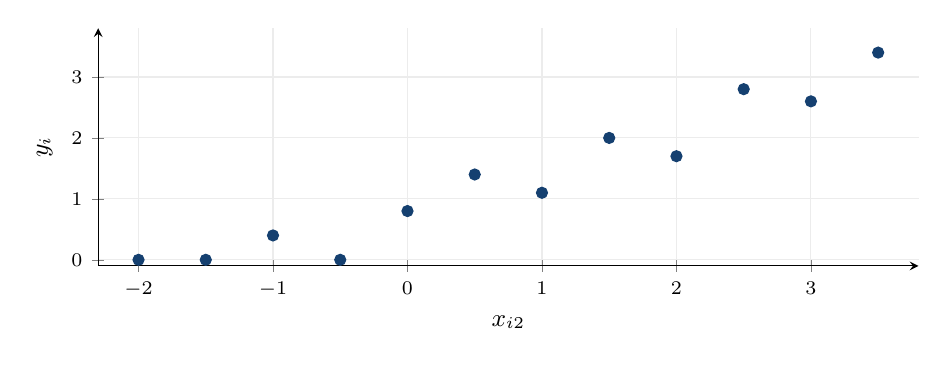
\begin{tikzpicture}\begin{axis}[base,width=12cm,height=4.6cm,xmin=-2.3,xmax=3.8,ymin=-.1,ymax=3.8,xlabel={$x_{i2}$},ylabel={$y_i$}]
\addplot[only marks,mark=*,azul] coordinates {(-2.00,0.00) (-1.50,0.00) (-1.00,0.40) (-0.50,0.00) (0.00,0.80) (0.50,1.40) (1.00,1.10) (1.50,2.00) (2.00,1.70) (2.50,2.80) (3.00,2.60) (3.50,3.40)};
\end{axis}\end{tikzpicture}
\caption{Ceros censurados y resultados positivos del laboratorio Tobit.}
\end{figure}

\clearpage
\section{Newton Tobit 0: probabilidades, dos scores y escala normalizada}\label{unidad106}
Se evalúa el modelo en un solo vector
de parámetros para las doce filas.
Las coordenadas y su reconstrucción son
\[
\begin{pmatrix}\beta_1/\sigma\\\beta_2/\sigma\\1/\sigma\end{pmatrix}=\begin{pmatrix}0\\0\\1.0000000\end{pmatrix},\quad\begin{pmatrix}\beta_1\\\beta_2\\\sigma\end{pmatrix}=\begin{pmatrix}0\\0\\1.0000000\end{pmatrix}.
\]

La tabla muestra el producto latente,
la probabilidad de censura y
las dos contribuciones al score
de coeficientes normalizados.
\begin{center}\small\begin{tabular}{rrrrr}\toprule
\(i\)&\(\beta_1+x_{i2}\beta_2\)&\(\Prob(Y_i=0\mid x_i)\)&score de \(\beta_1/\sigma\)&score de \(\beta_2/\sigma\)\\\midrule
1&0.0000000&0.5000000&-0.7978846&1.5957691\\
2&0.0000000&0.5000000&-0.7978846&1.1968268\\
3&0.0000000&0.5000000&0.4000000&-0.4000000\\
4&0.0000000&0.5000000&-0.7978846&0.3989423\\
5&0.0000000&0.5000000&0.8000000&0.0000000\\
6&0.0000000&0.5000000&1.4000000&0.7000000\\
7&0.0000000&0.5000000&1.1000000&1.1000000\\
8&0.0000000&0.5000000&2.0000000&3.0000000\\
9&0.0000000&0.5000000&1.7000000&3.4000000\\
10&0.0000000&0.5000000&2.8000000&7.0000000\\
11&0.0000000&0.5000000&2.6000000&7.8000000\\
12&0.0000000&0.5000000&3.4000000&11.9000000\\\bottomrule\end{tabular}\end{center}
Para ceros se multiplica
\(-\varphi(-\sum_jx_{ij}\beta_j/\sigma)/
\Phi(-\sum_jx_{ij}\beta_j/\sigma)\)
por la fila de datos.
Para positivos se multiplica
\(y_i/\sigma-\sum_jx_{ij}\beta_j/\sigma\).
La tercera coordenada del score
usa solamente positivos:
\[
\frac{\#\{i:y_i>0\}}{1/\sigma}
-\sum_{y_i>0}y_i\left(\frac{y_i}{\sigma}
-\sum_jx_{ij}\frac{\beta_j}{\sigma}\right).
\]
El score total y la curvatura positiva son
\[
\begin{pmatrix}10.9098593&10.4535209&-16.2000000\\10.4535209&40.1380285&-34.5000000\\-16.2000000&-34.5000000&46.0200000\end{pmatrix}\Delta^{(0)}=\begin{pmatrix}13.8063463\\37.6915382\\-28.0200000\end{pmatrix}.
\]

Resolver conserva sus términos cruzados:
\[
\Delta^{(0)}=\begin{pmatrix}1.1823278\\1.3090139\\0.7886721\end{pmatrix},\qquad\ell=-28.859888341.
\]

La propuesta se acepta solo con
inversa de escala positiva
y ascenso del objetivo original.
Al reducir un paso se modifica
todo el vector conjuntamente.

Una corrección final muy pequeña
puede aparecer como cero
en las cifras impresas.
La parada se verifica con
el score interno de mayor precisión,
no solo mirando la tabla.

\clearpage
\section{Newton Tobit 1: probabilidades, dos scores y escala normalizada}\label{unidad107}
Se evalúa el modelo en un solo vector
de parámetros para las doce filas.
Las coordenadas y su reconstrucción son
\[
\begin{pmatrix}\beta_1/\sigma\\\beta_2/\sigma\\1/\sigma\end{pmatrix}=\begin{pmatrix}1.1823278\\1.3090139\\1.7886721\end{pmatrix},\quad\begin{pmatrix}\beta_1\\\beta_2\\\sigma\end{pmatrix}=\begin{pmatrix}0.6610087\\0.7318356\\0.5590740\end{pmatrix}.
\]

La tabla muestra el producto latente,
la probabilidad de censura y
las dos contribuciones al score
de coeficientes normalizados.
\begin{center}\small\begin{tabular}{rrrrr}\toprule
\(i\)&\(\beta_1+x_{i2}\beta_2\)&\(\Prob(Y_i=0\mid x_i)\)&score de \(\beta_1/\sigma\)&score de \(\beta_2/\sigma\)\\\midrule
1&-0.8026625&0.9244561&-0.1539687&0.3079374\\
2&-0.4367447&0.7826555&-0.3756839&0.5635259\\
3&-0.0708269&0.5504056&0.8421549&-0.8421549\\
4&0.2950909&0.2988118&-1.1614918&0.5807459\\
5&0.6610087&0.1185378&0.2486099&0.0000000\\
6&1.0269265&0.0331171&0.6673062&0.3336531\\
7&1.3928443&0.0063631&-0.5238024&-0.5238024\\
8&1.7587621&0.0008280&0.4314955&0.6472433\\
9&2.1246799&0.0000722&-0.7596130&-1.5192261\\
10&2.4905977&0.0000042&0.5534193&1.3835483\\
11&2.8565155&0.0000002&-0.4588221&-1.3764662\\
12&3.2224333&0.0000000&0.3176087&1.1116304\\\bottomrule\end{tabular}\end{center}
Para ceros se multiplica
\(-\varphi(-\sum_jx_{ij}\beta_j/\sigma)/
\Phi(-\sum_jx_{ij}\beta_j/\sigma)\)
por la fila de datos.
Para positivos se multiplica
\(y_i/\sigma-\sum_jx_{ij}\beta_j/\sigma\).
La tercera coordenada del score
usa solamente positivos:
\[
\frac{\#\{i:y_i>0\}}{1/\sigma}
-\sum_{y_i>0}y_i\left(\frac{y_i}{\sigma}
-\sum_jx_{ij}\frac{\beta_j}{\sigma}\right).
\]
El score total y la curvatura positiva son
\[
\begin{pmatrix}10.4153829&11.4905497&-16.2000000\\11.4905497&38.1409328&-34.5000000\\-16.2000000&-34.5000000&39.8330732\end{pmatrix}\Delta^{(1)}=\begin{pmatrix}-0.3727875\\0.6666347\\3.1297146\end{pmatrix}.
\]

Resolver conserva sus términos cruzados:
\[
\Delta^{(1)}=\begin{pmatrix}0.6366140\\0.6046799\\0.8612019\end{pmatrix},\qquad\ell=-6.004521060.
\]

La propuesta se acepta solo con
inversa de escala positiva
y ascenso del objetivo original.
Al reducir un paso se modifica
todo el vector conjuntamente.

Una corrección final muy pequeña
puede aparecer como cero
en las cifras impresas.
La parada se verifica con
el score interno de mayor precisión,
no solo mirando la tabla.

\clearpage
\section{Newton Tobit 2: probabilidades, dos scores y escala normalizada}\label{unidad108}
Se evalúa el modelo en un solo vector
de parámetros para las doce filas.
Las coordenadas y su reconstrucción son
\[
\begin{pmatrix}\beta_1/\sigma\\\beta_2/\sigma\\1/\sigma\end{pmatrix}=\begin{pmatrix}1.8189418\\1.9136938\\2.6498740\end{pmatrix},\quad\begin{pmatrix}\beta_1\\\beta_2\\\sigma\end{pmatrix}=\begin{pmatrix}0.6864258\\0.7221829\\0.3773764\end{pmatrix}.
\]

La tabla muestra el producto latente,
la probabilidad de censura y
las dos contribuciones al score
de coeficientes normalizados.
\begin{center}\small\begin{tabular}{rrrrr}\toprule
\(i\)&\(\beta_1+x_{i2}\beta_2\)&\(\Prob(Y_i=0\mid x_i)\)&score de \(\beta_1/\sigma\)&score de \(\beta_2/\sigma\)\\\midrule
1&-0.7579401&0.9777020&-0.0542954&0.1085909\\
2&-0.3968486&0.8535082&-0.2688858&0.4033288\\
3&-0.0357571&0.5377441&1.1547015&-1.1547015\\
4&0.3253343&0.1943176&-1.4158340&0.7079170\\
5&0.6864258&0.0344602&0.3009573&0.0000000\\
6&1.0475173&0.0027534&0.9340348&0.4670174\\
7&1.4086087&0.0000947&-0.8177742&-0.8177742\\
8&1.7697002&0.0000014&0.6102655&0.9153982\\
9&2.1307917&0.0000000&-1.1415436&-2.2830872\\
10&2.4918831&0.0000000&0.8164709&2.0411772\\
11&2.8529746&0.0000000&-0.6703508&-2.0110524\\
12&3.2140661&0.0000000&0.4927015&1.7244552\\\bottomrule\end{tabular}\end{center}
Para ceros se multiplica
\(-\varphi(-\sum_jx_{ij}\beta_j/\sigma)/
\Phi(-\sum_jx_{ij}\beta_j/\sigma)\)
por la fila de datos.
Para positivos se multiplica
\(y_i/\sigma-\sum_jx_{ij}\beta_j/\sigma\).
La tercera coordenada del score
usa solamente positivos:
\[
\frac{\#\{i:y_i>0\}}{1/\sigma}
-\sum_{y_i>0}y_i\left(\frac{y_i}{\sigma}
-\sum_jx_{ij}\frac{\beta_j}{\sigma}\right).
\]
El score total y la curvatura positiva son
\[
\begin{pmatrix}10.2510597&11.8514144&-16.2000000\\11.8514144&37.4428745&-34.5000000\\-16.2000000&-34.5000000&38.3017168\end{pmatrix}\Delta^{(2)}=\begin{pmatrix}-0.0595525\\0.1012692\\0.7873462\end{pmatrix}.
\]

Resolver conserva sus términos cruzados:
\[
\Delta^{(2)}=\begin{pmatrix}0.2803793\\0.2479690\\0.3625013\end{pmatrix},\qquad\ell=-4.318740787.
\]

La propuesta se acepta solo con
inversa de escala positiva
y ascenso del objetivo original.
Al reducir un paso se modifica
todo el vector conjuntamente.

Una corrección final muy pequeña
puede aparecer como cero
en las cifras impresas.
La parada se verifica con
el score interno de mayor precisión,
no solo mirando la tabla.

\clearpage
\section{Newton Tobit 3: probabilidades, dos scores y escala normalizada}\label{unidad109}
Se evalúa el modelo en un solo vector
de parámetros para las doce filas.
Las coordenadas y su reconstrucción son
\[
\begin{pmatrix}\beta_1/\sigma\\\beta_2/\sigma\\1/\sigma\end{pmatrix}=\begin{pmatrix}2.0993211\\2.1616627\\3.0123752\end{pmatrix},\quad\begin{pmatrix}\beta_1\\\beta_2\\\sigma\end{pmatrix}=\begin{pmatrix}0.6968989\\0.7175941\\0.3319640\end{pmatrix}.
\]

La tabla muestra el producto latente,
la probabilidad de censura y
las dos contribuciones al score
de coeficientes normalizados.
\begin{center}\small\begin{tabular}{rrrrr}\toprule
\(i\)&\(\beta_1+x_{i2}\beta_2\)&\(\Prob(Y_i=0\mid x_i)\)&score de \(\beta_1/\sigma\)&score de \(\beta_2/\sigma\)\\\midrule
1&-0.7382893&0.9869259&-0.0340857&0.0681715\\
2&-0.3794922&0.8735166&-0.2376081&0.3564121\\
3&-0.0206952&0.5248546&1.2672917&-1.2672917\\
4&0.3381019&0.1542226&-1.5399637&0.7699818\\
5&0.6968989&0.0178943&0.3105791&0.0000000\\
6&1.0556960&0.0007360&1.0371728&0.5185864\\
7&1.4144931&0.0000102&-0.9473711&-0.9473711\\
8&1.7732901&0.0000000&0.6829352&1.0244028\\
9&2.1320872&0.0000000&-1.3016087&-2.6032174\\
10&2.4908842&0.0000000&0.9311726&2.3279316\\
11&2.8496813&0.0000000&-0.7521338&-2.2564013\\
12&3.2084784&0.0000000&0.5769350&2.0192726\\\bottomrule\end{tabular}\end{center}
Para ceros se multiplica
\(-\varphi(-\sum_jx_{ij}\beta_j/\sigma)/
\Phi(-\sum_jx_{ij}\beta_j/\sigma)\)
por la fila de datos.
Para positivos se multiplica
\(y_i/\sigma-\sum_jx_{ij}\beta_j/\sigma\).
La tercera coordenada del score
usa solamente positivos:
\[
\frac{\#\{i:y_i>0\}}{1/\sigma}
-\sum_{y_i>0}y_i\left(\frac{y_i}{\sigma}
-\sum_jx_{ij}\frac{\beta_j}{\sigma}\right).
\]
El score total y la curvatura positiva son
\[
\begin{pmatrix}10.2081043&11.9524101&-16.2000000\\11.9524101&37.2468282&-34.5000000\\-16.2000000&-34.5000000&38.0118006\end{pmatrix}\Delta^{(3)}=\begin{pmatrix}-0.0066846\\0.0104773\\0.0559116\end{pmatrix}.
\]

Resolver conserva sus términos cruzados:
\[
\Delta^{(3)}=\begin{pmatrix}0.0224409\\0.0207200\\0.0298406\end{pmatrix},\qquad\ell=-4.164610683.
\]

La propuesta se acepta solo con
inversa de escala positiva
y ascenso del objetivo original.
Al reducir un paso se modifica
todo el vector conjuntamente.

Una corrección final muy pequeña
puede aparecer como cero
en las cifras impresas.
La parada se verifica con
el score interno de mayor precisión,
no solo mirando la tabla.

\clearpage
\section{Newton Tobit 4: probabilidades, dos scores y escala normalizada}\label{unidad110}
Se evalúa el modelo en un solo vector
de parámetros para las doce filas.
Las coordenadas y su reconstrucción son
\[
\begin{pmatrix}\beta_1/\sigma\\\beta_2/\sigma\\1/\sigma\end{pmatrix}=\begin{pmatrix}2.1217620\\2.1823828\\3.0422158\end{pmatrix},\quad\begin{pmatrix}\beta_1\\\beta_2\\\sigma\end{pmatrix}=\begin{pmatrix}0.6974397\\0.7173662\\0.3287078\end{pmatrix}.
\]

La tabla muestra el producto latente,
la probabilidad de censura y
las dos contribuciones al score
de coeficientes normalizados.
\begin{center}\small\begin{tabular}{rrrrr}\toprule
\(i\)&\(\beta_1+x_{i2}\beta_2\)&\(\Prob(Y_i=0\mid x_i)\)&score de \(\beta_1/\sigma\)&score de \(\beta_2/\sigma\)\\\midrule
1&-0.7372927&0.9875517&-0.0326489&0.0652978\\
2&-0.3786096&0.8753009&-0.2347846&0.3521770\\
3&-0.0199265&0.5241694&1.2775071&-1.2775071\\
4&0.3387566&0.1513711&-1.5496736&0.7748368\\
5&0.6974397&0.0169289&0.3120107&0.0000000\\
6&1.0561228&0.0006569&1.0461488&0.5230744\\
7&1.4148059&0.0000084&-0.9577074&-0.9577074\\
8&1.7734890&0.0000000&0.6890955&1.0336432\\
9&2.1321720&0.0000000&-1.3147606&-2.6295213\\
10&2.4908551&0.0000000&0.9404854&2.3512134\\
11&2.8495382&0.0000000&-0.7591492&-2.2774475\\
12&3.2082213&0.0000000&0.5834321&2.0420123\\\bottomrule\end{tabular}\end{center}
Para ceros se multiplica
\(-\varphi(-\sum_jx_{ij}\beta_j/\sigma)/
\Phi(-\sum_jx_{ij}\beta_j/\sigma)\)
por la fila de datos.
Para positivos se multiplica
\(y_i/\sigma-\sum_jx_{ij}\beta_j/\sigma\).
La tercera coordenada del score
usa solamente positivos:
\[
\frac{\#\{i:y_i>0\}}{1/\sigma}
-\sum_{y_i>0}y_i\left(\frac{y_i}{\sigma}
-\sum_jx_{ij}\frac{\beta_j}{\sigma}\right).
\]
El score total y la curvatura positiva son
\[
\begin{pmatrix}10.2042894&11.9608574&-16.2000000\\11.9608574&37.2307913&-34.5000000\\-16.2000000&-34.5000000&37.9924392\end{pmatrix}\Delta^{(4)}=\begin{pmatrix}-0.0000448\\0.0000716\\0.0002903\end{pmatrix}.
\]

Resolver conserva sus términos cruzados:
\[
\Delta^{(4)}=\begin{pmatrix}0.0001167\\0.0001112\\0.0001583\end{pmatrix},\qquad\ell=-4.163739870.
\]

La propuesta se acepta solo con
inversa de escala positiva
y ascenso del objetivo original.
Al reducir un paso se modifica
todo el vector conjuntamente.

Una corrección final muy pequeña
puede aparecer como cero
en las cifras impresas.
La parada se verifica con
el score interno de mayor precisión,
no solo mirando la tabla.

\clearpage
\section{Newton Tobit 5: probabilidades, dos scores y escala normalizada}\label{unidad111}
Se evalúa el modelo en un solo vector
de parámetros para las doce filas.
Las coordenadas y su reconstrucción son
\[
\begin{pmatrix}\beta_1/\sigma\\\beta_2/\sigma\\1/\sigma\end{pmatrix}=\begin{pmatrix}2.1218787\\2.1824939\\3.0423741\end{pmatrix},\quad\begin{pmatrix}\beta_1\\\beta_2\\\sigma\end{pmatrix}=\begin{pmatrix}0.6974417\\0.7173654\\0.3286907\end{pmatrix}.
\]

La tabla muestra el producto latente,
la probabilidad de censura y
las dos contribuciones al score
de coeficientes normalizados.
\begin{center}\small\begin{tabular}{rrrrr}\toprule
\(i\)&\(\beta_1+x_{i2}\beta_2\)&\(\Prob(Y_i=0\mid x_i)\)&score de \(\beta_1/\sigma\)&score de \(\beta_2/\sigma\)\\\midrule
1&-0.7372891&0.9875551&-0.0326410&0.0652821\\
2&-0.3786064&0.8753112&-0.2347684&0.3521525\\
3&-0.0199237&0.5241672&1.2775649&-1.2775649\\
4&0.3387590&0.1513568&-1.5497228&0.7748614\\
5&0.6974417&0.0169240&0.3120207&0.0000000\\
6&1.0561244&0.0006565&1.0461982&0.5230991\\
7&1.4148071&0.0000084&-0.9577610&-0.9577610\\
8&1.7734898&0.0000000&0.6891287&1.0336931\\
9&2.1321725&0.0000000&-1.3148305&-2.6296609\\
10&2.4908552&0.0000000&0.9405341&2.3513353\\
11&2.8495379&0.0000000&-0.7591877&-2.2775630\\
12&3.2082206&0.0000000&0.5834647&2.0421264\\\bottomrule\end{tabular}\end{center}
Para ceros se multiplica
\(-\varphi(-\sum_jx_{ij}\beta_j/\sigma)/
\Phi(-\sum_jx_{ij}\beta_j/\sigma)\)
por la fila de datos.
Para positivos se multiplica
\(y_i/\sigma-\sum_jx_{ij}\beta_j/\sigma\).
La tercera coordenada del score
usa solamente positivos:
\[
\frac{\#\{i:y_i>0\}}{1/\sigma}
-\sum_{y_i>0}y_i\left(\frac{y_i}{\sigma}
-\sum_jx_{ij}\frac{\beta_j}{\sigma}\right).
\]
El score total y la curvatura positiva son
\[
\begin{pmatrix}10.2042670&11.9609052&-16.2000000\\11.9609052&37.2307014&-34.5000000\\-16.2000000&-34.5000000&37.9923380\end{pmatrix}\Delta^{(5)}=\begin{pmatrix}0\\0\\0\end{pmatrix}.
\]

Resolver conserva sus términos cruzados:
\[
\Delta^{(5)}=\begin{pmatrix}0\\0\\0\end{pmatrix},\qquad\ell=-4.163739845.
\]

La propuesta se acepta solo con
inversa de escala positiva
y ascenso del objetivo original.
Al reducir un paso se modifica
todo el vector conjuntamente.

Una corrección final muy pequeña
puede aparecer como cero
en las cifras impresas.
La parada se verifica con
el score interno de mayor precisión,
no solo mirando la tabla.

\clearpage
\section{Newton Tobit 6: probabilidades, dos scores y escala normalizada}\label{unidad112}
Se evalúa el modelo en un solo vector
de parámetros para las doce filas.
Las coordenadas y su reconstrucción son
\[
\begin{pmatrix}\beta_1/\sigma\\\beta_2/\sigma\\1/\sigma\end{pmatrix}=\begin{pmatrix}2.1218787\\2.1824939\\3.0423741\end{pmatrix},\quad\begin{pmatrix}\beta_1\\\beta_2\\\sigma\end{pmatrix}=\begin{pmatrix}0.6974417\\0.7173654\\0.3286907\end{pmatrix}.
\]

La tabla muestra el producto latente,
la probabilidad de censura y
las dos contribuciones al score
de coeficientes normalizados.
\begin{center}\small\begin{tabular}{rrrrr}\toprule
\(i\)&\(\beta_1+x_{i2}\beta_2\)&\(\Prob(Y_i=0\mid x_i)\)&score de \(\beta_1/\sigma\)&score de \(\beta_2/\sigma\)\\\midrule
1&-0.7372891&0.9875551&-0.0326410&0.0652821\\
2&-0.3786064&0.8753112&-0.2347684&0.3521525\\
3&-0.0199237&0.5241672&1.2775649&-1.2775649\\
4&0.3387590&0.1513568&-1.5497228&0.7748614\\
5&0.6974417&0.0169240&0.3120207&0.0000000\\
6&1.0561244&0.0006565&1.0461982&0.5230991\\
7&1.4148071&0.0000084&-0.9577610&-0.9577610\\
8&1.7734898&0.0000000&0.6891287&1.0336931\\
9&2.1321725&0.0000000&-1.3148305&-2.6296609\\
10&2.4908552&0.0000000&0.9405341&2.3513353\\
11&2.8495379&0.0000000&-0.7591877&-2.2775630\\
12&3.2082206&0.0000000&0.5834647&2.0421264\\\bottomrule\end{tabular}\end{center}
Para ceros se multiplica
\(-\varphi(-\sum_jx_{ij}\beta_j/\sigma)/
\Phi(-\sum_jx_{ij}\beta_j/\sigma)\)
por la fila de datos.
Para positivos se multiplica
\(y_i/\sigma-\sum_jx_{ij}\beta_j/\sigma\).
La tercera coordenada del score
usa solamente positivos:
\[
\frac{\#\{i:y_i>0\}}{1/\sigma}
-\sum_{y_i>0}y_i\left(\frac{y_i}{\sigma}
-\sum_jx_{ij}\frac{\beta_j}{\sigma}\right).
\]
El score total y la curvatura positiva son
\[
\begin{pmatrix}10.2042670&11.9609052&-16.2000000\\11.9609052&37.2307014&-34.5000000\\-16.2000000&-34.5000000&37.9923380\end{pmatrix}\Delta^{(6)}=\begin{pmatrix}0\\0\\0\end{pmatrix}.
\]

Resolver conserva sus términos cruzados:
\[
\Delta^{(6)}=\begin{pmatrix}0\\0\\0\end{pmatrix},\qquad\ell=-4.163739845.
\]

La propuesta se acepta solo con
inversa de escala positiva
y ascenso del objetivo original.
Al reducir un paso se modifica
todo el vector conjuntamente.

Una corrección final muy pequeña
puede aparecer como cero
en las cifras impresas.
La parada se verifica con
el score interno de mayor precisión,
no solo mirando la tabla.

\clearpage
\section{Tobit: raíz final y toda la covarianza de parámetros originales}\label{unidad113}
La solución final en los parámetros
del modelo latente es
\[
\begin{pmatrix}\widehat\beta_1\\\widehat\beta_2\\\widehat\sigma\end{pmatrix}\approx\begin{pmatrix}0.6974417\\0.7173654\\0.3286907\end{pmatrix}.
\]

Al sustituir en las tres ecuaciones
del score original, sus residuos
tienen valor absoluto menor que \(10^{-9}\).
El negativo de la Hessiana original es
\[
\begin{pmatrix}94.4511084&110.7106224&14.1584247\\110.7106224&344.6088775&-15.4896252\\14.1584247&-15.4896252&170.3722815\end{pmatrix}.
\]

La inversa local completa es
\[
\widehat{\Cov}
\begin{pmatrix}\widehat\beta_1\\\widehat\beta_2\\\widehat\sigma\end{pmatrix}
\approx\begin{pmatrix}0.0176286&-0.0057528&-0.0019880\\-0.0057528&0.0047911&0.0009137\\-0.0019880&0.0009137&0.0061178\end{pmatrix}.
\]

Su diagonal da varianzas aproximadas.
Sus raíces son
\[
\begin{pmatrix}0.1327729\\0.0692177\\0.0782162\end{pmatrix}.
\]

Las entradas de la última fila
contienen covarianzas de escala
con los dos coeficientes.
No se omiten al construir
incertidumbre de una probabilidad
o media Tobit.

También se verifica la inversa
en las coordenadas normalizadas.
El Jacobiano que reconstruye
los parámetros originales es
\[
\begin{pmatrix}0.3286907&0&-0.2292426\\0&0.3286907&-0.2357913\\0&0&-0.1080376\end{pmatrix}.
\]

Multiplicar Jacobiano, inversa de
curvatura normalizada y Jacobiano
transpuesto coincide con la
matriz original anterior,
salvo redondeo en la raíz.

Esta igualdad es una identidad
de cambio de coordenadas
en la solución.
La interpretación como covarianza
muestral del máximo es
una aproximación asintótica,
con las condiciones de
existencia y regularidad ya discutidas.

La raíz no se obtuvo tratando
los ceros como residuos
normales observados exactamente.
La primera parte de la
verosimilitud explica su
información de censura.

\clearpage
\section{Predicción Tobit de la fila 1: masa, media y dos varianzas}\label{unidad114}
El dato es \(x_i=(1,-2)\T\).
El producto latente conserva
sus dos multiplicaciones:
\[
(1)(0.69744172)+(-2)(0.71736539)=-0.73728907.
\]

Al dividir por escala se obtiene
\[
\frac{-0.73728907}{0.32869067}\approx-2.24310919.
\]

La masa censurada y la
probabilidad positiva son
\[
\Phi(-(-2.24310919))\approx0.98755511,\qquad\Phi(-2.24310919)\approx0.01244489.
\]

Primer momento, segundo momento
y varianza observados resultan
\[
\begin{aligned}
\E[Y_i\mid x_i]&\approx(-0.73728907)(0.01244489)+(0.32869067)(0.03223482)\\
&=0.00141981,\\
\E[Y_i^2\mid x_i]&\approx0.00029771,\\
\Var(Y_i\mid x_i)&\approx0.00029771-(0.00141981)^2=0.00029569.\end{aligned}
\]

Condicionado en positividad,
la media y varianza son
\[
0.11408753,\qquad 0.01090611.
\]

La incertidumbre de la media estimada
es otra varianza.
Su gradiente respecto de
\((\beta_1,\beta_2,\sigma)\) es
\[
\begin{pmatrix}0.0124449\\-0.0248898\\0.0322348\end{pmatrix}.
\]

Propagar ese vector con la
covarianza completa de parámetros
da varianza local de la
media estimada
\[
0.00001256,\quad\text{error estándar}\approx0.00354372.
\]

\begin{figure}[H]\centering
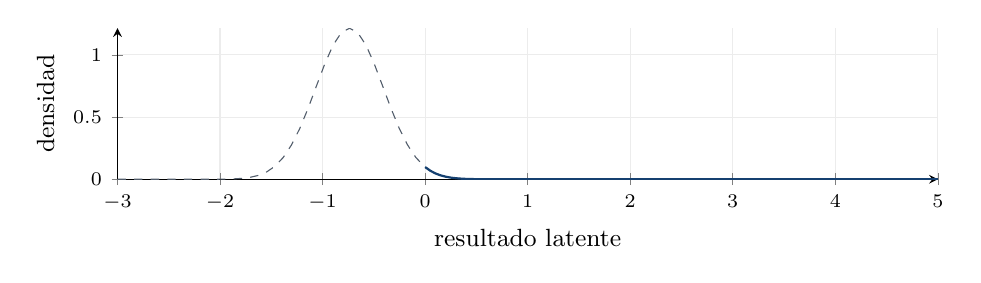
\begin{tikzpicture}\begin{axis}[base,width=12cm,height=3.5cm,xmin=-3,xmax=5,ymin=0,xlabel={resultado latente},ylabel={densidad}]
\addplot[gris,dashed,domain=-3:5]{exp(-((x-(-0.7372890670))/(0.3286906713))^2/2)/((0.3286906713)*sqrt(2*pi))};\addplot[azul,thick,domain=0:5]{exp(-((x-(-0.7372890670))/(0.3286906713))^2/2)/((0.3286906713)*sqrt(2*pi))};
\end{axis}\end{tikzpicture}
\caption{Densidad latente y parte continua observada: la cola negativa se acumula en una masa en cero.}
\end{figure}

La figura muestra densidades;
la masa del cero se calculó
por separado como probabilidad.
No se utiliza su altura
como si fuera una densidad continua.
El valor observado de la fila
no tiene que coincidir
con ninguna de sus medias.

\clearpage
\section{Predicción Tobit de la fila 3: masa, media y dos varianzas}\label{unidad115}
El dato es \(x_i=(1,-1)\T\).
El producto latente conserva
sus dos multiplicaciones:
\[
(1)(0.69744172)+(-1)(0.71736539)=-0.01992367.
\]

Al dividir por escala se obtiene
\[
\frac{-0.01992367}{0.32869067}\approx-0.06061527.
\]

La masa censurada y la
probabilidad positiva son
\[
\Phi(-(-0.06061527))\approx0.52416719,\qquad\Phi(-0.06061527)\approx0.47583281.
\]

Primer momento, segundo momento
y varianza observados resultan
\[
\begin{aligned}
\E[Y_i\mid x_i]&\approx(-0.01992367)(0.47583281)+(0.32869067)(0.39821005)\\
&=0.12140759,\\
\E[Y_i^2\mid x_i]&\approx0.04898893,\\
\Var(Y_i\mid x_i)&\approx0.04898893-(0.12140759)^2=0.03424913.\end{aligned}
\]

Condicionado en positividad,
la media y varianza son
\[
0.25514759,\qquad 0.03785379.
\]

La incertidumbre de la media estimada
es otra varianza.
Su gradiente respecto de
\((\beta_1,\beta_2,\sigma)\) es
\[
\begin{pmatrix}0.4758328\\-0.4758328\\0.3982101\end{pmatrix}.
\]

Propagar ese vector con la
covarianza completa de parámetros
da varianza local de la
media estimada
\[
0.00755175,\quad\text{error estándar}\approx0.08690080.
\]

\begin{figure}[H]\centering
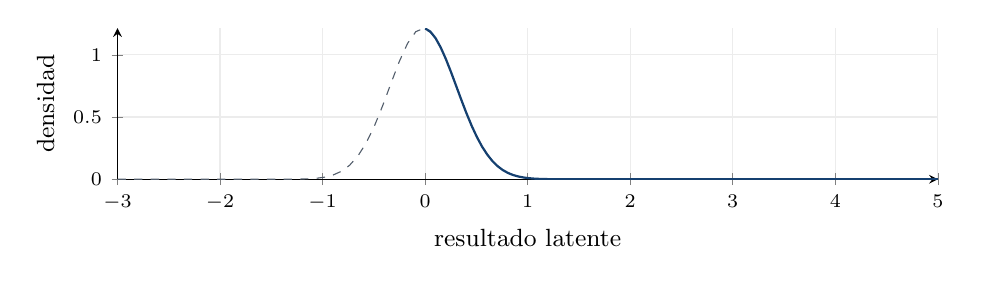
\begin{tikzpicture}\begin{axis}[base,width=12cm,height=3.5cm,xmin=-3,xmax=5,ymin=0,xlabel={resultado latente},ylabel={densidad}]
\addplot[gris,dashed,domain=-3:5]{exp(-((x-(-0.0199236728))/(0.3286906713))^2/2)/((0.3286906713)*sqrt(2*pi))};\addplot[azul,thick,domain=0:5]{exp(-((x-(-0.0199236728))/(0.3286906713))^2/2)/((0.3286906713)*sqrt(2*pi))};
\end{axis}\end{tikzpicture}
\caption{Densidad latente y parte continua observada: la cola negativa se acumula en una masa en cero.}
\end{figure}

La figura muestra densidades;
la masa del cero se calculó
por separado como probabilidad.
No se utiliza su altura
como si fuera una densidad continua.
El valor observado de la fila
no tiene que coincidir
con ninguna de sus medias.

\clearpage
\section{Predicción Tobit de la fila 5: masa, media y dos varianzas}\label{unidad116}
El dato es \(x_i=(1,0)\T\).
El producto latente conserva
sus dos multiplicaciones:
\[
(1)(0.69744172)+(0)(0.71736539)=0.69744172.
\]

Al dividir por escala se obtiene
\[
\frac{0.69744172}{0.32869067}\approx2.12187866.
\]

La masa censurada y la
probabilidad positiva son
\[
\Phi(-(2.12187866))\approx0.01692396,\qquad\Phi(2.12187866)\approx0.98307604.
\]

Primer momento, segundo momento
y varianza observados resultan
\[
\begin{aligned}
\E[Y_i\mid x_i]&\approx(0.69744172)(0.98307604)+(0.32869067)(0.04199843)\\
&=0.69944273,\\
\E[Y_i^2\mid x_i]&\approx0.59402968,\\
\Var(Y_i\mid x_i)&\approx0.59402968-(0.69944273)^2=0.10480954.\end{aligned}
\]

Condicionado en positividad,
la media y varianza son
\[
0.71148386,\qquad 0.09804680.
\]

La incertidumbre de la media estimada
es otra varianza.
Su gradiente respecto de
\((\beta_1,\beta_2,\sigma)\) es
\[
\begin{pmatrix}0.9830760\\0\\0.0419984\end{pmatrix}.
\]

Propagar ese vector con la
covarianza completa de parámetros
da varianza local de la
media estimada
\[
0.01688363,\quad\text{error estándar}\approx0.12993703.
\]

\begin{figure}[H]\centering
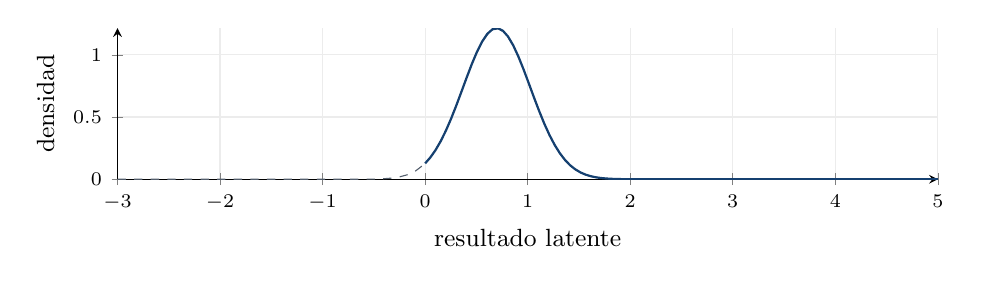
\begin{tikzpicture}\begin{axis}[base,width=12cm,height=3.5cm,xmin=-3,xmax=5,ymin=0,xlabel={resultado latente},ylabel={densidad}]
\addplot[gris,dashed,domain=-3:5]{exp(-((x-(0.6974417213))/(0.3286906713))^2/2)/((0.3286906713)*sqrt(2*pi))};\addplot[azul,thick,domain=0:5]{exp(-((x-(0.6974417213))/(0.3286906713))^2/2)/((0.3286906713)*sqrt(2*pi))};
\end{axis}\end{tikzpicture}
\caption{Densidad latente y parte continua observada: la cola negativa se acumula en una masa en cero.}
\end{figure}

La figura muestra densidades;
la masa del cero se calculó
por separado como probabilidad.
No se utiliza su altura
como si fuera una densidad continua.
El valor observado de la fila
no tiene que coincidir
con ninguna de sus medias.

\clearpage
\section{Predicción Tobit de la fila 7: masa, media y dos varianzas}\label{unidad117}
El dato es \(x_i=(1,1)\T\).
El producto latente conserva
sus dos multiplicaciones:
\[
(1)(0.69744172)+(1)(0.71736539)=1.41480712.
\]

Al dividir por escala se obtiene
\[
\frac{1.41480712}{0.32869067}\approx4.30437259.
\]

La masa censurada y la
probabilidad positiva son
\[
\Phi(-(4.30437259))\approx0.00000837,\qquad\Phi(4.30437259)\approx0.99999163.
\]

Primer momento, segundo momento
y varianza observados resultan
\[
\begin{aligned}
\E[Y_i\mid x_i]&\approx(1.41480712)(0.99999163)+(0.32869067)(0.00003782)\\
&=1.41480770,\\
\E[Y_i^2\mid x_i]&\approx2.10971665,\\
\Var(Y_i\mid x_i)&\approx2.10971665-(1.41480770)^2=0.10803583.\end{aligned}
\]

Condicionado en positividad,
la media y varianza son
\[
1.41481955,\qquad 0.10801997.
\]

La incertidumbre de la media estimada
es otra varianza.
Su gradiente respecto de
\((\beta_1,\beta_2,\sigma)\) es
\[
\begin{pmatrix}0.9999916\\0.9999916\\0.0000378\end{pmatrix}.
\]

Propagar ese vector con la
covarianza completa de parámetros
da varianza local de la
media estimada
\[
0.01091383,\quad\text{error estándar}\approx0.10446929.
\]

\begin{figure}[H]\centering
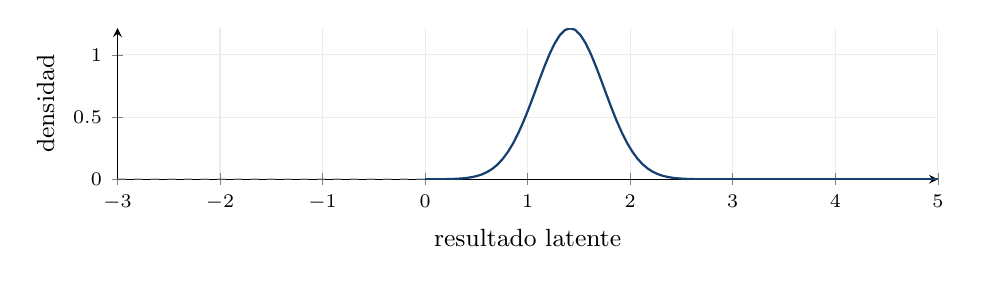
\begin{tikzpicture}\begin{axis}[base,width=12cm,height=3.5cm,xmin=-3,xmax=5,ymin=0,xlabel={resultado latente},ylabel={densidad}]
\addplot[gris,dashed,domain=-3:5]{exp(-((x-(1.4148071155))/(0.3286906713))^2/2)/((0.3286906713)*sqrt(2*pi))};\addplot[azul,thick,domain=0:5]{exp(-((x-(1.4148071155))/(0.3286906713))^2/2)/((0.3286906713)*sqrt(2*pi))};
\end{axis}\end{tikzpicture}
\caption{Densidad latente y parte continua observada: la cola negativa se acumula en una masa en cero.}
\end{figure}

La figura muestra densidades;
la masa del cero se calculó
por separado como probabilidad.
No se utiliza su altura
como si fuera una densidad continua.
El valor observado de la fila
no tiene que coincidir
con ninguna de sus medias.

\clearpage
\section{Predicción Tobit de la fila 9: masa, media y dos varianzas}\label{unidad118}
El dato es \(x_i=(1,2)\T\).
El producto latente conserva
sus dos multiplicaciones:
\[
(1)(0.69744172)+(2)(0.71736539)=2.13217251.
\]

Al dividir por escala se obtiene
\[
\frac{2.13217251}{0.32869067}\approx6.48686651.
\]

La masa censurada y la
probabilidad positiva son
\[
\Phi(-(6.48686651))\approx0.00000000,\qquad\Phi(6.48686651)\approx1.00000000.
\]

Primer momento, segundo momento
y varianza observados resultan
\[
\begin{aligned}
\E[Y_i\mid x_i]&\approx(2.13217251)(1.00000000)+(0.32869067)(0.00000000)\\
&=2.13217251,\\
\E[Y_i^2\mid x_i]&\approx4.65419717,\\
\Var(Y_i\mid x_i)&\approx4.65419717-(2.13217251)^2=0.10803756.\end{aligned}
\]

Condicionado en positividad,
la media y varianza son
\[
2.13217251,\qquad 0.10803756.
\]

La incertidumbre de la media estimada
es otra varianza.
Su gradiente respecto de
\((\beta_1,\beta_2,\sigma)\) es
\[
\begin{pmatrix}1.0000000\\2.0000000\\0\end{pmatrix}.
\]

Propagar ese vector con la
covarianza completa de parámetros
da varianza local de la
media estimada
\[
0.01378171,\quad\text{error estándar}\approx0.11739555.
\]

\begin{figure}[H]\centering
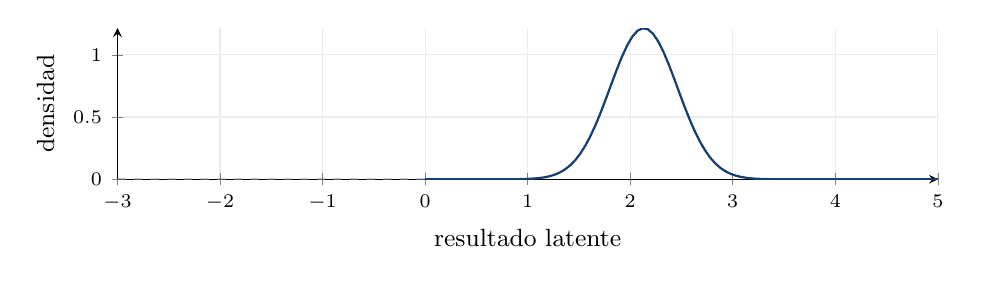
\begin{tikzpicture}\begin{axis}[base,width=12cm,height=3.5cm,xmin=-3,xmax=5,ymin=0,xlabel={resultado latente},ylabel={densidad}]
\addplot[gris,dashed,domain=-3:5]{exp(-((x-(2.1321725096))/(0.3286906713))^2/2)/((0.3286906713)*sqrt(2*pi))};\addplot[azul,thick,domain=0:5]{exp(-((x-(2.1321725096))/(0.3286906713))^2/2)/((0.3286906713)*sqrt(2*pi))};
\end{axis}\end{tikzpicture}
\caption{Densidad latente y parte continua observada: la cola negativa se acumula en una masa en cero.}
\end{figure}

La figura muestra densidades;
la masa del cero se calculó
por separado como probabilidad.
No se utiliza su altura
como si fuera una densidad continua.
El valor observado de la fila
no tiene que coincidir
con ninguna de sus medias.

\clearpage
\section{Predicción Tobit de la fila 12: masa, media y dos varianzas}\label{unidad119}
El dato es \(x_i=(1,3.5)\T\).
El producto latente conserva
sus dos multiplicaciones:
\[
(1)(0.69744172)+(3.5)(0.71736539)=3.20822060.
\]

Al dividir por escala se obtiene
\[
\frac{3.20822060}{0.32869067}\approx9.76060741.
\]

La masa censurada y la
probabilidad positiva son
\[
\Phi(-(9.76060741))\approx0.00000000,\qquad\Phi(9.76060741)\approx1.00000000.
\]

Primer momento, segundo momento
y varianza observados resultan
\[
\begin{aligned}
\E[Y_i\mid x_i]&\approx(3.20822060)(1.00000000)+(0.32869067)(0.00000000)\\
&=3.20822060,\\
\E[Y_i^2\mid x_i]&\approx10.40071698,\\
\Var(Y_i\mid x_i)&\approx10.40071698-(3.20822060)^2=0.10803756.\end{aligned}
\]

Condicionado en positividad,
la media y varianza son
\[
3.20822060,\qquad 0.10803756.
\]

La incertidumbre de la media estimada
es otra varianza.
Su gradiente respecto de
\((\beta_1,\beta_2,\sigma)\) es
\[
\begin{pmatrix}1.0000000\\3.5000000\\0\end{pmatrix}.
\]

Propagar ese vector con la
covarianza completa de parámetros
da varianza local de la
media estimada
\[
0.03604971,\quad\text{error estándar}\approx0.18986761.
\]

\begin{figure}[H]\centering
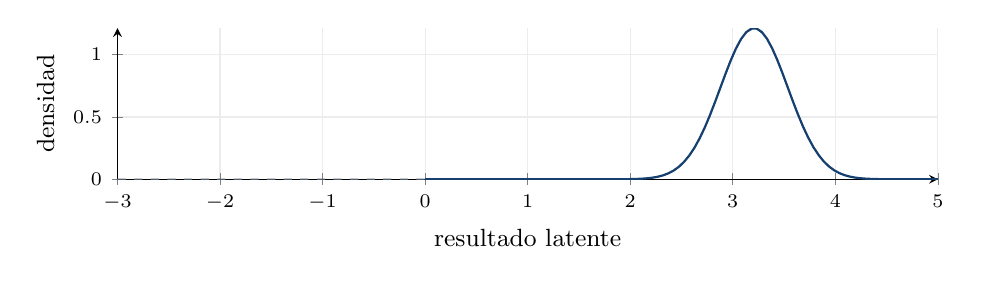
\begin{tikzpicture}\begin{axis}[base,width=12cm,height=3.5cm,xmin=-3,xmax=5,ymin=0,xlabel={resultado latente},ylabel={densidad}]
\addplot[gris,dashed,domain=-3:5]{exp(-((x-(3.2082206008))/(0.3286906713))^2/2)/((0.3286906713)*sqrt(2*pi))};\addplot[azul,thick,domain=0:5]{exp(-((x-(3.2082206008))/(0.3286906713))^2/2)/((0.3286906713)*sqrt(2*pi))};
\end{axis}\end{tikzpicture}
\caption{Densidad latente y parte continua observada: la cola negativa se acumula en una masa en cero.}
\end{figure}

La figura muestra densidades;
la masa del cero se calculó
por separado como probabilidad.
No se utiliza su altura
como si fuera una densidad continua.
El valor observado de la fila
no tiene que coincidir
con ninguna de sus medias.

\clearpage
\section{Problema Tobit: comparar MCO de todos, MCO de positivos y máximo censurado}\label{unidad120}
Sobre los mismos doce datos se pueden
calcular tres reglas distintas.
MCO de todos los observados trata
cada cero como magnitud exacta.
MCO de positivos elimina la
información de las filas censuradas.
Tobit utiliza masas y densidades
según el tipo de fila.

Las soluciones numéricas son
\[
\begin{aligned}
\widehat\beta_{\mathrm{MCO,todos}}&=\begin{pmatrix}0.8811189\\0.6251748\end{pmatrix},\\
\widehat\beta_{\mathrm{MCO,positivos}}&=\begin{pmatrix}0.8690323\\0.6445161\end{pmatrix},\\
\widehat\beta_{\mathrm{Tobit}}&=\begin{pmatrix}0.6974417\\0.7173654\end{pmatrix}.\end{aligned}
\]

El primer MCO aproxima una
media observada no lineal.
El segundo aproxima una
media condicionada positiva que
incluye una razón normal.
El tercero estima los
coeficientes de la ecuación latente
bajo su modelo de censura.

Las diferencias de una realización
no prueban por sí solas
el sesgo de cada procedimiento.
La inconsistencia de una regresión
lineal para coeficientes latentes
se deduce de que la
media observable no coincide
con la suma latente,
salvo circunstancias especiales.

Los tres pueden producir
predicciones e interpretaciones distintas.
No se compara un coeficiente
de proyección observada con
uno latente como si ambos
respondieran exactamente
a la misma pregunta.

\begin{ejemplo}[Datos sin censura casi frecuente]
Si la probabilidad de censura
es despreciable en todas las filas,
Tobit se aproxima al
modelo normal no censurado.
Con censura importante,
la diferencia de mecanismos
se vuelve relevante.
\end{ejemplo}
El ejercicio permite reconstruir
qué información utiliza cada regla.
El modelo de aplicación
debe determinar cuál
cantidad se busca estimar
antes de escoger por
un resultado numérico atractivo.

\clearpage
\addcontentsline{toc}{part}{Heckman: selección, dos etapas y verosimilitud conjunta}
\pdfbookmark[0]{Heckman: selección, dos etapas y verosimilitud conjunta}{parte121}
\section{Modelo de selección: dos ecuaciones y un resultado que puede faltar}\label{unidad121}
La ecuación de resultado potencial es
\[
Y_i^\ast=\sum_{j=1}^kx_{ij}\beta_j+\varepsilon_i.
\]
La ecuación de selección es
\[
S_i=\mathbf1\left\{\sum_{l=1}^qz_{il}\gamma_l+\nu_i>0\right\}.
\]
Se observa \(Y_i^\ast\) como \(y_i\)
únicamente si \(S_i=1\).
Los regresores de selección deben
estar disponibles también en las filas
con resultado no observado.

Condicionados en \(x_i,z_i\), los dos errores
siguen la normal bivariada construida antes:
\[
\Cov\begin{pmatrix}\varepsilon_i\\\nu_i\end{pmatrix}
=\begin{pmatrix}\sigma^2&\rho\sigma\\\rho\sigma&1\end{pmatrix}.
\]
La correlación \(\rho\) permite
que la selección de errores de
participación cambie la media
del error de resultado observado.

La escala de \(\nu_i\) está normalizada.
Multiplicar una ecuación latente binaria
por una constante positiva no cambia
su indicador. Por eso su escala
no se identifica separadamente
sin una normalización.

Un valor no observado no es
un cero salarial ni un cero censurado.
El evento \(S_i=0\) informa
sobre la ecuación de selección;
no revela que \(Y_i^\ast\le0\).
El resultado seleccionado puede
tener cualquier signo bajo
la ecuación normal.

\begin{ejemplo}[Ecuación de log ingreso]
En aplicaciones salariales, el resultado
puede ser log ingreso por hora
y la selección disponibilidad de
ingreso y horas válidos.
El conjunto que participa en
la selección es más amplio
que el conjunto con ingreso observado.
\end{ejemplo}
El modelo de Heckman formaliza
selección como problema de especificación
de una media condicionada \cite{heckman1979}.
La corrección de este tratado se
deducirá de su hipótesis normal,
sin asumir que funcione para
cualquier mecanismo de ausencia.

Definir quién pertenece a la
población y qué implica \(S_i=1\)
es parte del modelo.
La técnica no decide automáticamente
qué registros debieron llegar
a cada ecuación.

\clearpage
\section{Probabilidad de selección y el conjunto de datos de primera etapa}\label{unidad122}
Mantener fijos los regresores convierte
selección en un umbral del error:
\[
S_i=1\Longleftrightarrow
\nu_i>-\sum_lz_{il}\gamma_l.
\]
La normal estándar produce
\[
\Prob(S_i=1\mid z_i)
=\Phi\left(\sum_lz_{il}\gamma_l\right),
\]
\[
\Prob(S_i=0\mid z_i)
=\Phi\left(-\sum_lz_{il}\gamma_l\right).
\]
La suma de ambas es uno.

El indicador se observa en
todas las personas de la
población usada en selección.
Su verosimilitud probit combina
los dos eventos en todas esas filas.
Si primero se eliminan todos
los no seleccionados, solo queda
un indicador constante igual a uno.

La matriz de selección es
\[
Z=\begin{pmatrix}
z_{11}&\cdots&z_{1q}\\
\vdots&&\vdots\\
z_{n1}&\cdots&z_{nq}
\end{pmatrix}.
\]
Su rango permite distinguir
coeficientes de selección.
Puede incluir columnas presentes
en la ecuación de resultado
y otras excluidas de ella
con una justificación sustantiva.

\begin{ejemplo}[Intercepto único]
Si hay \(m\) seleccionados de \(n\)
y \(0<m<n\), el probit de
intercepto único satisface
\(\Phi(\widehat\gamma_1)=m/n\).
Su raíz es el cuantil normal
de esa proporción.
\end{ejemplo}
La ecuación binaria modela
disponibilidad de resultado,
no su nivel.
Un buen ajuste de esa probabilidad
no valida por sí solo
la ecuación salarial ni
la exclusión de variables.

La consistencia requiere que
el modelo de probabilidad
sea apropiado y que
las observaciones aporten
información suficiente.
Separación o todos los indicadores
iguales pueden impedir
un máximo probit finito.

Se verificará existencia del
probit del laboratorio antes
de usar sus coeficientes
para construir la segunda etapa.

\clearpage
\section{Derivar la media del error seleccionado por esperanza iterada}\label{unidad123}
La normal bivariada implica
\[
\E[\varepsilon_i\mid\nu_i,x_i,z_i]=\rho\sigma\nu_i.
\]
Seleccionar restringe \(\nu_i\)
a superar su umbral.
La ley de esperanza iterada da
\[
\begin{aligned}
\E[\varepsilon_i\mid x_i,z_i,S_i=1]
&=\E[\E[\varepsilon_i\mid\nu_i,x_i,z_i]\mid x_i,z_i,S_i=1]\\
&=\rho\sigma\E[\nu_i\mid z_i,S_i=1].
\end{aligned}
\]
La media truncada ya fue integrada,
por lo que
\[
\boxed{
\E[\varepsilon_i\mid x_i,z_i,S_i=1]
=\rho\sigma
\frac{\varphi(\sum_lz_{il}\gamma_l)}
{\Phi(\sum_lz_{il}\gamma_l)}}.
\]
No se asumió que el error
de resultado tenga media cero
entre quienes se seleccionan.

Si \(\rho=0\), la media es cero
bajo esta distribución conjunta.
Si \(\rho>0\), es positiva.
Si \(\rho<0\), es negativa.
La razón normal es siempre positiva,
pero el coeficiente puede tener
cualquiera de esos signos.

\begin{ejemplo}[Selección a probabilidad un medio]
Con índice cero, \(\rho=.5,\sigma=2\),
la media del error observado es
\(\sqrt{2/\pi}\approx.79788456\).
No es un aumento causal
del producto lineal de ingresos;
es composición del error observado.
\end{ejemplo}
La corrección se obtiene de
la covarianza entre errores y
del evento truncado.
No aparece por agregar una
variable correlacionada cualquiera
a una regresión.

Una hipótesis de normalidad
solo marginal de cada error
no garantiza toda esta deducción:
se requiere la estructura conjunta
que produjo la media condicional
lineal en \(\nu_i\).

En otra distribución conjunta,
la función de corrección puede
ser distinta de la razón
normal que se está usando.

\clearpage
\section{Varianza del error seleccionado: deducir los dos componentes}\label{unidad124}
La construcción bivariada es
\[
\varepsilon_i=\rho\sigma\nu_i
+\sigma\sqrt{1-\rho^2}\,u_i,
\]
con \(u_i\) normal independiente.
Seleccionar depende de \(\nu_i\),
y deja intacta la distribución de \(u_i\).
La varianza condicionada es
\[
\rho^2\sigma^2\Var(\nu_i\mid z_i,S_i=1)
+\sigma^2(1-\rho^2).
\]
El cruce es cero por independencia
y media cero del segundo error.

Sustituir la varianza truncada produce
\[
\begin{aligned}
\Var(\varepsilon_i\mid x_i,z_i,S_i=1)
=\sigma^2\Bigg\{1-&\rho^2
\frac{\varphi(\sum_lz_{il}\gamma_l)}
{\Phi(\sum_lz_{il}\gamma_l)}\\
&\cdot\left[
\sum_lz_{il}\gamma_l+
\frac{\varphi(\sum_lz_{il}\gamma_l)}
{\Phi(\sum_lz_{il}\gamma_l)}
\right]\Bigg\}.
\end{aligned}
\]
El factor de razón por corchete
está entre cero y uno.
Por eso la varianza está entre
\(\sigma^2(1-\rho^2)\) y \(\sigma^2\)
para argumentos finitos.

La dependencia del índice de
selección genera heterocedasticidad
en la segunda etapa.
Una misma escala latente
no implica iguales varianzas
de errores observados.

\begin{ejemplo}[Índice cero]
El factor de corrección es \(2/\pi\).
Con \(\sigma=2,\rho=.6\),
la varianza seleccionada es
\[
4[1-.36(2/\pi)]\approx3.08326753.
\]
\end{ejemplo}
El valor cambia con cada fila.
Una varianza cercana a la
escala latente puede ocurrir
si selección es casi universal.
Con selección muy rara,
la parte compartida de error
varía poco alrededor de su
nueva media, pero la parte
independiente sigue aportando.

Estas dos partes son esenciales
para estimar incertidumbre
de coeficientes de resultado
sin suponer homocedasticidad
de la muestra seleccionada.

\clearpage
\section{Media de no seleccionados y cancelación de la media poblacional}\label{unidad125}
Para \(S_i=0\), el error de selección
cumple \(\nu_i\le-\sum_lz_{il}\gamma_l\).
La integral de primer momento
de la cola inferior es
el negativo de su densidad de frontera.
Así,
\[
\E[\nu_i\mid z_i,S_i=0]
=-\frac{\varphi(\sum_lz_{il}\gamma_l)}
{\Phi(-\sum_lz_{il}\gamma_l)}.
\]
Multiplicar por la media condicional
bivariada produce
\[
\E[\varepsilon_i\mid x_i,z_i,S_i=0]
=-\rho\sigma
\frac{\varphi(\sum_lz_{il}\gamma_l)}
{\Phi(-\sum_lz_{il}\gamma_l)}.
\]

La ley de esperanza total
comprueba que las dos medias
seleccionadas se compensan:
\[
\begin{aligned}
&\Phi(\sum_lz_{il}\gamma_l)
\left[\rho\sigma\frac{\varphi(\sum_lz_{il}\gamma_l)}
{\Phi(\sum_lz_{il}\gamma_l)}\right]\\
&+\Phi(-\sum_lz_{il}\gamma_l)
\left[-\rho\sigma\frac{\varphi(\sum_lz_{il}\gamma_l)}
{\Phi(-\sum_lz_{il}\gamma_l)}\right]=0.
\end{aligned}
\]
El error original mantiene media cero
dado los regresores.
Las medias condicionadas pueden
ser distintas y no nulas.

\begin{ejemplo}[Selección rara]
Si pocos se seleccionan y
la correlación es positiva,
los seleccionados pueden tener
un error medio grande positivo.
La mayoría no seleccionada
tiene una media negativa
de menor magnitud que
compensa al ponderar por probabilidades.
\end{ejemplo}
No observar el resultado de
los no seleccionados impide
calcular directamente su media
a partir de esas respuestas.
La expresión pertenece al modelo
y no a una comparación
empírica observada completa.

La deducción también muestra
que un error con media cero
en población puede generar
sesgo al analizar solo
un subconjunto condicionado.

\clearpage
\section{Sesgo de MCO seleccionado: desplegar la proyección omitida}\label{unidad126}
Entre seleccionados, la media de resultado es
\[
\sum_jx_{ij}\beta_j+
\rho\sigma\frac{\varphi(\sum_lz_{il}\gamma_l)}
{\Phi(\sum_lz_{il}\gamma_l)}.
\]
Si se ajusta solo la parte
lineal en \(x_i\), se omite
la segunda función.

Condicionemos en un patrón de
selección y en todos los regresores.
Si la matriz de filas seleccionadas
tiene rango completo, la esperanza
del MCO sin corrección satisface
\[
\begin{aligned}
\E[\widehat\beta_{\mathrm{MCO}}\mid X,Z,S]-\beta
={}&\rho\sigma
\left[\sum_{S_i=1}x_ix_i\T\right]^{-1}\\
&\cdot\sum_{S_i=1}x_i
\frac{\varphi(\sum_lz_{il}\gamma_l)}
{\Phi(\sum_lz_{il}\gamma_l)}.
\end{aligned}
\]
Cada coordenada del sesgo
depende de la proyección
de la razón normal sobre
todas las columnas incluidas.

Una correlación positiva entre errores
no implica que todas las
pendientes tengan sesgo positivo.
La razón es positiva,
pero su relación con
cada regresor y la inversa
del producto cruzado pueden
cambiar signos de coordenadas.

\begin{ejemplo}[Razón constante]
Si todas las filas seleccionadas
tienen exactamente el mismo índice,
la corrección es una constante.
Con intercepto, puede desplazar
solo su coeficiente sin
alterar pendientes identificables.
Sin variación de la razón,
su coeficiente propio no se
distingue del intercepto.
\end{ejemplo}
La dirección de un sesgo
no se memoriza a partir
del nombre Heckman.
Se deduce de la matriz
de proyección y del mecanismo
de selección concreto.

La falta de resultado entre
no seleccionados no se corrige
simplemente agrupando errores
o agregando efectos de año.
La media condicionada omitida
es otro problema del modelo.

\clearpage
\section{Ecuación corregida: definir el coeficiente de Mills y el nuevo error}\label{unidad127}
Definamos el coeficiente
\(\delta=\rho\sigma\).
Es un parámetro de la ecuación
de media seleccionada,
no un dato renombrado.
El nuevo error es
el error original menos
su media condicionada:
\[
\varepsilon_i-
\delta\frac{\varphi(\sum_lz_{il}\gamma_l)}
{\Phi(\sum_lz_{il}\gamma_l)}.
\]
Por construcción tiene
esperanza cero entre seleccionados,
dados sus regresores.

La ecuación corregida es
\[
\begin{aligned}
Y_i^\ast
={}&\sum_jx_{ij}\beta_j
+\delta\frac{\varphi(\sum_lz_{il}\gamma_l)}
{\Phi(\sum_lz_{il}\gamma_l)}\\
&+\left[
\varepsilon_i-\delta
\frac{\varphi(\sum_lz_{il}\gamma_l)}
{\Phi(\sum_lz_{il}\gamma_l)}
\right],\qquad S_i=1.
\end{aligned}
\]
La corchetera final no se elimina
como si fuera un número conocido:
es el error aleatorio seleccionado
centrado en su media.

Su varianza es
\[
\sigma^2-\delta^2
\frac{\varphi(\sum_lz_{il}\gamma_l)}
{\Phi(\sum_lz_{il}\gamma_l)}
\left[
\sum_lz_{il}\gamma_l+
\frac{\varphi(\sum_lz_{il}\gamma_l)}
{\Phi(\sum_lz_{il}\gamma_l)}
\right].
\]
Restar una media fija
dado los regresores no
cambia la varianza condicionada.

\begin{ejemplo}[Qué se prueba con \(\delta=0\)]
Bajo el modelo normal,
la escala positiva implica
\(\delta=0\Longleftrightarrow\rho=0\).
La corrección de media desaparece.
Una prueba sobre ese coeficiente
necesita errores estándar
que contemplen su regresor generado.
\end{ejemplo}
La segunda etapa estima
\(\beta\) y \(\delta\)
como coeficientes de una
ecuación de media.
Reconstruir \(\rho=\delta/\sigma\)
necesita estimar también escala,
con su incertidumbre correspondiente.

\clearpage
\section{Restricción de exclusión: variación que identifica la corrección}\label{unidad128}
Una variable puede entrar en \(z_i\)
para explicar selección y
estar excluida de \(x_i\)
en la ecuación de resultado.
La exclusión exige una justificación:
condicionando en los controles,
esa variable no debe afectar
directamente la ecuación de resultado.

Su variación permite que
la probabilidad de selección
y la razón normal cambien
sin reproducir únicamente
la misma suma de regresores
de resultado.
Esto ayuda a distinguir
\(\delta\) de los coeficientes
de la ecuación principal.

Sin una exclusión, el modelo
normal puede identificarse
por su forma funcional no lineal
en situaciones con suficiente variación.
Pero la razón puede parecer
casi lineal en los regresores
sobre el rango de una muestra.
La distinción puede ser débil
y muy sensible a la hipótesis normal.

\begin{ejemplo}[Un instrumento de selección]
Una característica que modifica
costos de participación podría
afectar disponibilidad de resultado.
Su exclusión de la ecuación
de ingreso requiere argumentar
por qué no modifica directamente
productividad o salario potencial.
El ejemplo no valida automáticamente
esa variable en una base real.
\end{ejemplo}
Una variable excluida casi sin
efecto en selección aporta
poca variación útil.
Tener una columna adicional
no basta: importan su
relevancia, su rango y
la relación con las
otras columnas.

La exclusión de Heckman
no equivale a un instrumento
que corrige automáticamente
endogeneidad de todos los
regresores de ingreso.
El modelo todavía necesita
sus hipótesis de exogeneidad
condicionada para la ecuación
de resultado potencial.

La calidad de identificación
debe evaluarse antes de
interpretar un coeficiente
de Mills grande o impreciso
como evidencia económica concluyente.

\clearpage
\section{Dos etapas: construir la matriz seleccionada sin abreviar Mills}\label{unidad129}
Primero se estima \(\gamma\)
con todos los indicadores de selección.
Después, en cada fila seleccionada,
se evalúa
\[
\frac{\varphi(\sum_lz_{il}\widehat\gamma_l)}
{\Phi(\sum_lz_{il}\widehat\gamma_l)}.
\]
La segunda etapa utiliza las
filas seleccionadas con una
columna adicional completa.

Con intercepto y una pendiente,
el diseño es
\[
\begin{pmatrix}
1&x_{i2}&
\frac{\varphi(\sum_lz_{il}\widehat\gamma_l)}
{\Phi(\sum_lz_{il}\widehat\gamma_l)}\\
\vdots&\vdots&\vdots
\end{pmatrix}_{S_i=1}.
\]
El vector de coeficientes es
\((\beta_1,\beta_2,\delta)\T\).

Las seis sumas distintas de
su producto cruzado son
\[
\begin{gathered}
\sum_{S_i=1}1,\quad
\sum_{S_i=1}x_{i2},\quad
\sum_{S_i=1}x_{i2}^2,\\
\sum_{S_i=1}
\frac{\varphi(\sum_lz_{il}\widehat\gamma_l)}
{\Phi(\sum_lz_{il}\widehat\gamma_l)},\quad
\sum_{S_i=1}x_{i2}
\frac{\varphi(\sum_lz_{il}\widehat\gamma_l)}
{\Phi(\sum_lz_{il}\widehat\gamma_l)},\\
\sum_{S_i=1}\left[
\frac{\varphi(\sum_lz_{il}\widehat\gamma_l)}
{\Phi(\sum_lz_{il}\widehat\gamma_l)}
\right]^2.
\end{gathered}
\]
Se colocan en las nueve
posiciones por simetría,
como en cualquier producto
de tres columnas.
El lado derecho suma cada
una de las columnas por \(y_i\).

La raíz lineal de esta etapa
no resuelve una ecuación
Tobit de censura.
Se está ajustando una
media condicionada en selección
que se derivó con otro mecanismo.

El regresor adicional es estimado.
La covarianza de los coeficientes
debe estudiar tanto
la dispersión del nuevo error
como la incertidumbre de
\(\widehat\gamma\).

\clearpage
\section{Primera etapa conocida: esperanza exacta de los coeficientes corregidos}\label{unidad130}
Supongamos temporalmente que \(\gamma\)
es conocido y el patrón seleccionado
produce un diseño ampliado de rango completo.
La columna normal es entonces
fija condicionado en \(X,Z,S\).
La media seleccionada es
exactamente lineal en ese diseño.

La expansión de la segunda etapa es
\[
\begin{aligned}
&\begin{pmatrix}\widehat\beta\\\widehat\delta\end{pmatrix}
-\begin{pmatrix}\beta\\\delta\end{pmatrix}\\
&=
\left[\sum_{S_i=1}
\begin{pmatrix}x_i\\\varphi(\sum_lz_{il}\gamma_l)/\Phi(\sum_lz_{il}\gamma_l)\end{pmatrix}
(x_i\T,\varphi(\sum_lz_{il}\gamma_l)/\Phi(\sum_lz_{il}\gamma_l))
\right]^{-1}\\
&\quad\cdot\sum_{S_i=1}
\begin{pmatrix}x_i\\\varphi(\sum_lz_{il}\gamma_l)/\Phi(\sum_lz_{il}\gamma_l)\end{pmatrix}
\left[\varepsilon_i-
\delta\frac{\varphi(\sum_lz_{il}\gamma_l)}
{\Phi(\sum_lz_{il}\gamma_l)}\right].
\end{aligned}
\]
Cada nuevo error tiene
media condicionada cero.
Tomar esperanza demuestra
insesgamiento exacto condicionado
en esta situación ideal.

La afirmación está condicionada
en un patrón con rango.
Un patrón que selecciona
demasiadas pocas filas puede
impedir calcular una raíz.
No se afirma existencia
en todos los patrones posibles.

\begin{ejemplo}[Un límite]
Con solo intercepto y
un índice de selección constante,
la columna normal es constante.
No se distinguen intercepto y
coeficiente de corrección.
La matriz ampliada es singular.
\end{ejemplo}
Al sustituir \(\gamma\) por
un estimador aleatorio,
la misma prueba finita ya
no es automática.
La columna generada cambia
con las respuestas de selección.

La consistencia de dos etapas
se justificará por convergencia
de esa primera etapa
y por las ecuaciones conjuntas,
no declarando conocida una
columna que realmente fue estimada.

\clearpage
\section{Covarianza corregida con selección conocida: heterocedasticidad fila a fila}\label{unidad131}

Supongamos selección conocida y un patrón observado de rango completo.
Cada fila ampliada contiene los regresores de resultado y su
razón normal calculada con el parámetro verdadero.
El error seleccionado centrado tiene varianza distinta por fila.

La propagación completa de todos los coeficientes
de resultado y del coeficiente de corrección es
\[
\begin{aligned}
\Cov\!\left(\begin{pmatrix}\widehat\beta\\\widehat\delta\end{pmatrix}
\Bigm|X,Z,S\right)
={}&\left[\sum_{S_i=1}\begin{pmatrix}x_i\\\frac{\varphi(\sum_lz_{il}\gamma_l)}{\Phi(\sum_lz_{il}\gamma_l)}\end{pmatrix}\left(x_i\T,\ \frac{\varphi(\sum_lz_{il}\gamma_l)}{\Phi(\sum_lz_{il}\gamma_l)}\right)\right]^{-1}\\
&\cdot\Bigg\{\sum_{S_i=1}
\left[\sigma^2-\delta^2\frac{\varphi(\sum_lz_{il}\gamma_l)}{\Phi(\sum_lz_{il}\gamma_l)}\left[\sum_lz_{il}\gamma_l+\frac{\varphi(\sum_lz_{il}\gamma_l)}{\Phi(\sum_lz_{il}\gamma_l)}\right]\right]\\
&\qquad\quad\cdot\begin{pmatrix}x_i\\\frac{\varphi(\sum_lz_{il}\gamma_l)}{\Phi(\sum_lz_{il}\gamma_l)}\end{pmatrix}\left(x_i\T,\ \frac{\varphi(\sum_lz_{il}\gamma_l)}{\Phi(\sum_lz_{il}\gamma_l)}\right)\Bigg\}\\
&\cdot\left[\sum_{S_i=1}\begin{pmatrix}x_i\\\frac{\varphi(\sum_lz_{il}\gamma_l)}{\Phi(\sum_lz_{il}\gamma_l)}\end{pmatrix}\left(x_i\T,\ \frac{\varphi(\sum_lz_{il}\gamma_l)}{\Phi(\sum_lz_{il}\gamma_l)}\right)\right]^{-1}.
\end{aligned}
\]

No se asignó una letra nueva a la razón ni a la matriz de
productos cruzados. Las dos inversas contienen todas las
sumas de datos de las filas seleccionadas.

La matriz central pondera cada producto exterior
por su varianza seleccionada. Con intercepto y una pendiente,
su entrada \((1,3)\) suma la razón por esa varianza;
su entrada \((3,3)\) suma la razón al cuadrado por la varianza.
La entrada de pendiente por corrección también conserva
cada \(x_{i2}\).

Esta es una identidad finita si los parámetros de selección
y la varianza del modelo son conocidos y las filas latentes
son independientes. Al estimar esos parámetros,
se necesitan los términos de incertidumbre heredada.

La fórmula homocedástica ordinaria de MCO ampliado no reemplaza
esta operación: la selección ha cambiado la varianza entre filas.
Con varianzas conocidas se puede construir un ajuste generalizado;
con varianzas estimadas se trata de otro procedimiento factible
cuyo alcance estadístico debe justificarse.


\clearpage
\section{Recuperar escala y correlación: la corrección de segundos momentos}\label{unidad132}
La varianza de error seleccionado
puede escribirse como \(\sigma^2\)
menos \(\delta^2\) por el
factor normal de truncamiento.
Por ello, promediar solamente
residuos cuadrados seleccionados
puede subestimar la escala latente.

Una regla consistente de momentos
en dos etapas agrega ese
factor estimado al promedio
de residuos cuadrados:
\[
\begin{aligned}
\widehat\sigma^2
={}&\frac1{\#\{i:S_i=1\}}\sum_{S_i=1}
\Bigg\{
\left[y_i-\sum_jx_{ij}\widehat\beta_j
-\widehat\delta
\frac{\varphi(\sum_lz_{il}\widehat\gamma_l)}
{\Phi(\sum_lz_{il}\widehat\gamma_l)}\right]^2\\
&+\widehat\delta^2
\frac{\varphi(\sum_lz_{il}\widehat\gamma_l)}
{\Phi(\sum_lz_{il}\widehat\gamma_l)}
\left[
\sum_lz_{il}\widehat\gamma_l+
\frac{\varphi(\sum_lz_{il}\widehat\gamma_l)}
{\Phi(\sum_lz_{il}\widehat\gamma_l)}
\right]\Bigg\}.
\end{aligned}
\]
Su justificación utiliza consistencia
y condiciones de promedios,
no un insesgamiento exacto
de cada término estimado en muestra finita.

Reconstruir la correlación usa
\(\widehat\rho=\widehat\delta/\widehat\sigma\).
Una segunda etapa sin restricciones
puede producir \(|\widehat\rho|>1\)
en muestras pequeñas.
Eso indica incompatibilidad de
esa reconstrucción con el
espacio paramétrico bivariado;
no se llama correlación válida.

\begin{ejemplo}[Parámetros conocidos]
Si se conociera la razón,
\(\delta\) y la media exacta,
sumar al cuadrado del error
centrado el factor \(\delta^2\)
corregido tendría esperanza \(\sigma^2\)
en cada fila seleccionada.
Al estimarlos, aparece
incertidumbre adicional.
\end{ejemplo}
Una corrección de grados de libertad
para residuos de una regresión
no elimina todos esos
términos de estimación generada.

Los intervalos de \(\rho\) requieren
propagar la covarianza de
\(\delta,\sigma\).
No se divide simplemente
un error estándar de
\(\widehat\delta\) por una
escala considerada fija.

\clearpage
\section{Información del probit: esperanza y covarianza de sus coeficientes}\label{unidad133}
El score de selección es
la suma de \(z_i\) por
los dos cocientes normales
ponderados por \(S_i\) y \(1-S_i\).
Su esperanza en el
modelo correcto es cero:
\[
\Phi(t)\frac{\varphi(t)}{\Phi(t)}
-\Phi(-t)\frac{\varphi(-t)}{\Phi(-t)}=0.
\]
En esta comprobación \(t\)
es un argumento escalar;
en cada fila se sustituye
por \(\sum_lz_{il}\gamma_l\).

La covarianza de score por fila es
\[
\frac{\varphi(\sum_lz_{il}\gamma_l)^2}
{\Phi(\sum_lz_{il}\gamma_l)\Phi(-\sum_lz_{il}\gamma_l)}
\,z_iz_i\T.
\]
Se deduce sumando los
cuadrados de las dos
contribuciones por sus
probabilidades y usando
que estas suman uno.

La información esperada total
suma esas matrices sobre
todas las filas, seleccionadas
y no seleccionadas.
Bajo regularidad, su inversa
proporciona una covarianza
asintótica para \(\widehat\gamma\).

Las entradas de esa matriz
conservan productos \(z_{il}z_{ir}\).
Con tres columnas,
hay tres varianzas y
tres covarianzas distintas.
Las coordenadas estimadas
no son independientes por
usar respuestas binarias independientes.

\begin{ejemplo}[Índice cero]
La razón de información
es \((1/(2\pi))/(1/4)=2/\pi\).
Coincide con el negativo
de la Hessiana por fila
en el inicio cero.
Fuera de ese punto,
la curvatura observada
puede diferir de su esperanza.
\end{ejemplo}
La aproximación requiere un
máximo finito identificado.
La misma inversión no
soluciona separación de la
ecuación de selección.

La primera etapa aportará
su score y su información
a la covarianza conjunta
de los coeficientes de
resultado y corrección.

\clearpage
\section{Jacobiano de todas las razones estimadas respecto de selección}\label{unidad134}
La razón de la fila \(i\)
depende de las \(q\)
coordenadas de \(\gamma\).
Su derivada respecto de \(\gamma_l\) es
\[
\begin{aligned}
-&\frac{\varphi(\sum_hz_{ih}\gamma_h)}
{\Phi(\sum_hz_{ih}\gamma_h)}
\left[
\sum_hz_{ih}\gamma_h+
\frac{\varphi(\sum_hz_{ih}\gamma_h)}
{\Phi(\sum_hz_{ih}\gamma_h)}
\right]z_{il}.
\end{aligned}
\]
El Jacobiano tiene \(n\) filas
y \(q\) columnas.
La fila \(i\) es el
factor escalar negativo por \(z_i\T\).

Para una perturbación \(\Delta\gamma\),
el cambio de cada razón
es aproximadamente la suma
de sus \(q\) derivadas
por las perturbaciones.
No se mueve solamente
el intercepto de selección
si las otras coordenadas
también fueron estimadas.

La covarianza aproximada de
las razones de dos filas
es el producto de sus
gradientes, la covarianza
de \(\widehat\gamma\) y
el gradiente transpuesto
de la otra fila.
Puede ser no nula,
aunque sus indicadores de
selección sean independientes
dados los parámetros verdaderos.

\begin{ejemplo}[Primera etapa compartida]
Dos individuos utilizan el
mismo \(\widehat\gamma\).
Un aumento de su intercepto
reduce ambas razones,
con sensibilidad distinta
según cada índice.
Ese cambio compartido puede
correlacionar las columnas generadas.
\end{ejemplo}
Esta propagación explica el
origen de incertidumbre heredada,
pero todavía no es la
covarianza completa de la
segunda etapa.
Hay que considerar cómo
la columna entra en
sus ecuaciones normales.

La siguiente deducción mantendrá
el cambio de la razón
dentro del residuo y
también dentro de la
fila ampliada cuando corresponda.

\clearpage
\section{Ecuaciones apiladas: resultados, corrección y selección}\label{unidad135}
La segunda etapa tiene \(k+1\)
ecuaciones. Para cada coeficiente
de resultado se utiliza
\[
\sum_i S_i x_{ij}\left[
y_i-\sum_hx_{ih}\beta_h
-\delta\frac{\varphi(\sum_lz_{il}\gamma_l)}
{\Phi(\sum_lz_{il}\gamma_l)}\right]=0.
\]
La ecuación de \(\delta\) es
\[
\sum_i S_i
\frac{\varphi(\sum_lz_{il}\gamma_l)}
{\Phi(\sum_lz_{il}\gamma_l)}
\left[
y_i-\sum_hx_{ih}\beta_h
-\delta\frac{\varphi(\sum_lz_{il}\gamma_l)}
{\Phi(\sum_lz_{il}\gamma_l)}\right]=0.
\]
El producto \(S_i\) indica que
solo se usan resultados disponibles.
No se necesita asignar
un resultado cero ficticio
a los no seleccionados.

Debajo se apilan las \(q\)
ecuaciones de score probit
que usan todos los indicadores.
El vector conjunto de parámetros
es \((\beta\T,\delta,\gamma\T)\T\).
Su dimensión es \(k+1+q\).

Las ecuaciones de selección
no dependen de \(\beta,\delta\)
en el procedimiento de dos etapas.
Su bloque de derivadas hacia
esas coordenadas es cero.
Las ecuaciones de resultados
sí dependen de \(\gamma\),
porque cambian las razones normales.

\begin{ejemplo}[Dos regresores de resultado y tres de selección]
La matriz conjunta tiene dimensión seis.
Los tres primeros parámetros son
intercepto, pendiente y coeficiente
de corrección; los tres
restantes son de selección.
\end{ejemplo}
Esta estructura triangular
permite resolver primero
selección y luego resultados,
pero no hace independientes
los cambios estimados.

Su covarianza conjunta se
obtendrá al linearizar
todo el sistema,
con los bloques cruzados
que aquí se han identificado.

\clearpage
\section{Derivar el bloque cruzado: la razón cambia en dos lugares}\label{unidad136}
En una ecuación de \(\beta_j\),
la fila \(x_{ij}\) es fija.
Derivar respecto de \(\gamma_l\)
actúa únicamente sobre la
razón dentro del residuo:
\[
-\delta\sum_iS_ix_{ij}
\frac{\partial}{\partial\gamma_l}
\frac{\varphi(\sum_hz_{ih}\gamma_h)}
{\Phi(\sum_hz_{ih}\gamma_h)}.
\]
Sustituir su derivada completa
conserva cada \(z_{il}\)
y cada factor normal.

La ecuación de \(\delta\)
contiene la razón fuera
y dentro del residuo.
La regla del producto genera
\[
\begin{aligned}
&\sum_iS_i
\frac{\partial}{\partial\gamma_l}
\frac{\varphi(\sum_hz_{ih}\gamma_h)}
{\Phi(\sum_hz_{ih}\gamma_h)}
\left[
y_i-\sum_jx_{ij}\beta_j
-\delta\frac{\varphi(\sum_hz_{ih}\gamma_h)}
{\Phi(\sum_hz_{ih}\gamma_h)}
\right]\\
&-\delta\sum_iS_i
\frac{\varphi(\sum_hz_{ih}\gamma_h)}
{\Phi(\sum_hz_{ih}\gamma_h)}
\frac{\partial}{\partial\gamma_l}
\frac{\varphi(\sum_hz_{ih}\gamma_h)}
{\Phi(\sum_hz_{ih}\gamma_h)}.
\end{aligned}
\]
La primera línea no es
automáticamente cero en muestra.

En los parámetros verdaderos,
su esperanza es cero por
la media condicional cero
del error seleccionado centrado.
Esa simplificación poblacional
no autoriza a borrar
todas sus realizaciones numéricas.

La derivada de segunda etapa
respecto de \((\beta,\delta)\)
es el negativo del
producto cruzado ampliado.
La de primera etapa
respecto de \(\gamma\)
es la Hessiana probit.

\begin{ejemplo}[Un residuo observado]
Un residuo distinto de cero
multiplica el cambio de
la fila de Mills en
la ecuación de \(\delta\).
Ignorarlo modifica el
Jacobiano exacto del
sistema muestral.
\end{ejemplo}
Estos bloques permiten verificar
por diferencias finitas cada
entrada de la matriz conjunta,
antes de invertirla para
calcular dispersión.

\clearpage
\section{Covarianza entre momentos de ambas etapas: demostrar el cero poblacional}\label{unidad137}
El momento de resultados por fila
es la fila ampliada por
el error seleccionado centrado,
multiplicado por \(S_i\).
El score probit depende
solo de \(S_i,z_i\).
Condicionemos en \(x_i,z_i,S_i\).

Si \(S_i=0\), el momento
de resultado es cero.
Si \(S_i=1\), el error
centrado tiene media cero.
La fila ampliada y
el score de selección
son constantes dados esos
condicionantes.

Por esperanza iterada,
el producto cruzado de ambos
momentos tiene esperanza cero
bajo el modelo correcto.
Como ambas medias de momentos
son cero, su covarianza
poblacional cruzada es cero.

Esto no significa que
los estimadores sean independientes.
La segunda etapa responde
al cambio de \(\gamma\)
a través de su Jacobiano
cruzado, aun cuando las
perturbaciones originales de
momentos sean ortogonales.

La covarianza central de
momentos de resultado es
la esperanza de
\[
\begin{aligned}
S_i&
\begin{pmatrix}x_i\\\varphi(\sum_lz_{il}\gamma_l)/\Phi(\sum_lz_{il}\gamma_l)\end{pmatrix}
(x_i\T,\varphi(\sum_lz_{il}\gamma_l)/\Phi(\sum_lz_{il}\gamma_l))\\
&\cdot\Var(\varepsilon_i\mid x_i,z_i,S_i=1).
\end{aligned}
\]
La de selección es
la información probit
deducida anteriormente.

\begin{ejemplo}[Muestra finita]
Los productos de residuos
por score pueden sumar
un número distinto de cero
en la muestra observada.
La identidad de esperanza
no implica una cancelación
fila por fila de esos productos.
\end{ejemplo}
Bajo especificación incorrecta,
la media condicional del
error centrado puede no ser cero
y la ortogonalidad puede fallar.
Un sándwich conjunto empírico
puede conservar esos cruces
en lugar de imponer
el cero poblacional.

\clearpage
\section{Covarianza de dos etapas: linearizar todo el sistema}\label{unidad138}
Taylor de las ecuaciones de resultados
produce su momento verdadero,
menos el producto cruzado
ampliado por el cambio
de \((\beta,\delta)\),
más el bloque cruzado
por el cambio de \(\gamma\).

Las ecuaciones probit producen
su score verdadero más
su Hessiana por
\(\widehat\gamma-\gamma\).
Resolver este segundo sistema
y sustituirlo en el primero
muestra dos fuentes de
variación en resultados:
sus momentos seleccionados y
el score de primera etapa.

Bajo el modelo correcto,
la ortogonalidad poblacional
demostrada antes elimina
el cruce entre esas dos
fuentes originales.
La matriz central de
la covarianza de segunda etapa
contiene entonces su propia
dispersión más el bloque
de sensibilidad por la
covarianza de primera etapa
por la sensibilidad transpuesta.

Las dos matrices exteriores
son las inversas del
producto cruzado ampliado.
Toda esa expresión tiene
\(k+1\) filas y columnas.
No se reduce a
una sola inversa homocedástica.

En formulación completamente general,
se usa el Jacobiano conjunto
de las \(k+1+q\) ecuaciones:
\[
\begin{aligned}
&\left[\frac{\partial\,\text{ecuaciones conjuntas}}
{\partial(\beta\T,\delta,\gamma\T)}\right]^{-1}\\
&\quad\cdot
\left[\sum_i
(\text{vector de momentos de la fila }i)
(\text{vector de momentos de la fila }i)\T\right]\\
&\quad\cdot
\left[\frac{\partial\,\text{ecuaciones conjuntas}}
{\partial(\beta\T,\delta,\gamma\T)}\right]^{-\mathsf T}.
\end{aligned}
\]
Sus entradas y vectores son
las sumas completas escritas
en las unidades anteriores.

\begin{ejemplo}[Referencia]
Si \(\gamma\) fuese conocido,
su cambio aleatorio sería cero.
Desaparecería el término heredado,
recuperando la covarianza
de selección conocida.
\end{ejemplo}
La fórmula es asintótica para
el procedimiento real estimado.
La corrección de dispersión
no garantiza exactitud de
momentos finitos de una
raíz no lineal completa.

\clearpage
\section{Matriz conjunta de seis parámetros: sus tres bloques no nulos}\label{unidad139}
Con dos coeficientes de resultado, \(\delta\)
y tres de selección, el Jacobiano
tiene seis filas y columnas.
El bloque superior izquierdo es
el negativo de
\[
\sum_iS_i
\begin{pmatrix}
1&x_{i2}&\frac{\varphi(\sum_lz_{il}\gamma_l)}{\Phi(\sum_lz_{il}\gamma_l)}\\
x_{i2}&x_{i2}^2&x_{i2}\frac{\varphi(\sum_lz_{il}\gamma_l)}{\Phi(\sum_lz_{il}\gamma_l)}\\
\frac{\varphi(\sum_lz_{il}\gamma_l)}{\Phi(\sum_lz_{il}\gamma_l)}
&x_{i2}\frac{\varphi(\sum_lz_{il}\gamma_l)}{\Phi(\sum_lz_{il}\gamma_l)}
&\left[\frac{\varphi(\sum_lz_{il}\gamma_l)}{\Phi(\sum_lz_{il}\gamma_l)}\right]^2
\end{pmatrix}.
\]
El bloque inferior izquierdo es cero,
porque la primera etapa no
usa parámetros de resultados.

La entrada \((j,l)\), \(j=1,2\),
del bloque superior derecho es
\[
-\delta\sum_iS_ix_{ij}z_{il}
\left(\frac{\varphi}{\Phi}\right)'
\left(\sum_hz_{ih}\gamma_h\right).
\]
La fila tercera de ese bloque
contiene el producto de derivada
por residuo y el cambio
de la razón dentro del residuo,
desarrollados en la unidad anterior.

El bloque inferior derecho es
\[
\sum_i
\left[
S_i\left(\frac{\varphi}{\Phi}\right)'(\sum_lz_{il}\gamma_l)
+(1-S_i)\left(\frac{\varphi}{\Phi}\right)'(-\sum_lz_{il}\gamma_l)
\right]z_iz_i\T.
\]
La notación de derivada de la
función normal significa la
expresión completa de Mills
ya deducida; cada argumento
conserva su suma de datos.

La matriz puede ser no simétrica,
porque estas son ecuaciones de
dos etapas, no el gradiente
de una sola verosimilitud conjunta.
Por eso el sándwich general
usa inversa transpuesta
en el último factor.

La matriz central suma los
productos exteriores de los
seis momentos por fila.
Incluye cruces muestrales entre etapas.
El laboratorio imprimirá ambos
bloques y su matriz de
covarianza numérica completa.

\clearpage
\section{Bootstrap de dos etapas: qué debe volver a estimarse}\label{unidad140}
Un remuestreo que busca reproducir
la variación del procedimiento
debe reconstruir las dos etapas.
En cada muestra replicada se
estima nuevamente el probit,
se calculan nuevamente todas
las razones y se estima
la ecuación de resultados.

Mantener fija la primera
columna de Mills de la
muestra original reproduce
el problema de primera etapa
conocida, no el procedimiento
completo que se aplicó
a los datos originales.

Para filas independientes,
el remuestreo debe conservar
el registro completo:
regresores de ambas ecuaciones,
indicador y resultado disponible.
El resultado ausente sigue
ausente si su indicador es cero.
No se rellena con un
cero salarial inventado.

Si hay grupos dependientes,
un remuestreo de grupos
puede ser apropiado bajo
sus condiciones asintóticas.
Remuestrear registros aislados
dentro de esa dependencia
no reproduce necesariamente
el mecanismo relevante.

\begin{ejemplo}[Una réplica]
Si el probit de una réplica
cambia su coeficiente excluido,
cambian las razones de
todas las filas seleccionadas.
Eso puede mover \(\widehat\delta\)
y también las pendientes
de resultado por sus cruces.
\end{ejemplo}
El bootstrap no garantiza
validez en toda muestra pequeña.
Una réplica puede presentar
separación o falta de rango.
Su frecuencia informa sobre
fragilidad del procedimiento,
y no debe ocultarse
sustituyendo siempre una
raíz arbitraria sin declaración.

Las varianzas empíricas entre
replicaciones son aproximaciones
de remuestreo.
Se distinguen de las
identidades de covarianza
con parámetros de selección
conocidos y de las
matrices asintóticas analíticas.

\clearpage
\section{Heckman por máxima verosimilitud: deducir la densidad conjunta}\label{unidad141}
En una fila seleccionada, el resultado
determina el error de resultado
\(e=y_i-\sum_jx_{ij}\beta_j\).
Su densidad marginal es
\(\varphi(e/\sigma)/\sigma\).
Condicionado en ese error,
la selección utiliza la
normal condicional de \(\nu_i\):
\[
\nu_i\mid\varepsilon_i=e
\sim\mathcal N(\rho e/\sigma,1-\rho^2).
\]
La probabilidad de superar
\(-\sum_lz_{il}\gamma_l\)
es
\[
\Phi\left(
\frac{\sum_lz_{il}\gamma_l+
\rho(y_i-\sum_jx_{ij}\beta_j)/\sigma}
{\sqrt{1-\rho^2}}\right).
\]

Multiplicar densidad marginal por
probabilidad condicional produce
la densidad conjunta de
resultado y selección:
\[
\boxed{
\frac1\sigma
\varphi\left(\frac{y_i-\sum_jx_{ij}\beta_j}{\sigma}\right)
\Phi\left(
\frac{\sum_lz_{il}\gamma_l+
\rho(y_i-\sum_jx_{ij}\beta_j)/\sigma}
{\sqrt{1-\rho^2}}\right)}.
\]
Para \(S_i=0\), se integra
todo resultado no observado,
y queda
\(\Phi(-\sum_lz_{il}\gamma_l)\).

La densidad de resultado
condicionado en selección sí
divide la expresión seleccionada
por \(\Phi(\sum_lz_{il}\gamma_l)\).
La verosimilitud conjunta ya
incluye el evento de selección;
no agrega ese denominador
otra vez.

\begin{ejemplo}[Independencia]
Si \(\rho=0\), la probabilidad
condicional seleccionada se
reduce a \(\Phi(\sum_lz_{il}\gamma_l)\),
independiente del resultado.
La densidad conjunta factoriza.
\end{ejemplo}
Integrar la densidad conjunta
sobre todos los resultados
seleccionados recupera
la probabilidad de selección.
Es una comprobación de
normalización del mecanismo,
no una densidad normal
ordinaria de la muestra seleccionada.

\clearpage
\section{Log-verosimilitud conjunta Heckman: tres partes en una fila seleccionada}\label{unidad142}
La suma completa es
\[
\begin{aligned}
\ell(\beta,\gamma,\sigma,\rho)
={}&\sum_{S_i=0}\log\Phi(-\sum_lz_{il}\gamma_l)\\
&+\sum_{S_i=1}\Bigg[
-\log\sigma-\frac12\log(2\pi)
-\frac{(y_i-\sum_jx_{ij}\beta_j)^2}{2\sigma^2}\\
&\qquad+
\log\Phi\left(
\frac{\sum_lz_{il}\gamma_l+
\rho(y_i-\sum_jx_{ij}\beta_j)/\sigma}
{\sqrt{1-\rho^2}}\right)
\Bigg].
\end{aligned}
\]
La fila seleccionada combina
Jacobiano de escala, densidad
normal del resultado y
probabilidad condicional de selección.

Los parámetros de resultado
intervienen también en esa
última acumulada.
Por ello el máximo conjunto
no equivale a ajustar
independientemente una normal
a los resultados seleccionados
cuando \(\rho\ne0\).

La primera etapa de dos etapas
estima selección marginal.
La verosimilitud conjunta
aprovecha también la relación
entre resultado y selección
a través de la correlación.

\begin{ejemplo}[Resultado favorable y correlación positiva]
Un error de resultado alto
incrementa la media condicional
del error de selección.
Con \(\rho>0\),
la probabilidad de observar
esa fila depende de su
magnitud de resultado.
\end{ejemplo}
El espacio paramétrico interior
exige \(\sigma>0\) y \(|\rho|<1\).
Las expresiones con raíz
de \(1-\rho^2\) no
se evalúan fuera de
esas restricciones.

La existencia, estabilidad y
posibles máximos deben
analizarse en un ajuste concreto.
No se atribuye concavidad
global de todos los parámetros
a una función que contiene
estos términos de escala
y correlación no lineales.

\clearpage
\section{Score conjunto de cada coeficiente de resultado}\label{unidad143}
En una fila seleccionada,
la parte normal produce
\(x_{ij}(y_i-\sum_hx_{ih}\beta_h)/\sigma^2\).
La parte acumulada requiere
derivar su argumento completo
respecto del coeficiente:
\[
-\frac{\rho x_{ij}}{\sigma\sqrt{1-\rho^2}}.
\]
La regla de \(\log\Phi\)
multiplica esa derivada
por la razón normal
en el mismo argumento.

El score total de \(\beta_j\) es
\[
\begin{aligned}
\sum_{S_i=1}\Bigg[
&\frac{x_{ij}(y_i-\sum_hx_{ih}\beta_h)}{\sigma^2}\\
&-\frac{\rho x_{ij}}{\sigma\sqrt{1-\rho^2}}
\frac{
\varphi\left(\frac{\sum_lz_{il}\gamma_l+
\rho(y_i-\sum_hx_{ih}\beta_h)/\sigma}{\sqrt{1-\rho^2}}\right)}
{\Phi\left(\frac{\sum_lz_{il}\gamma_l+
\rho(y_i-\sum_hx_{ih}\beta_h)/\sigma}{\sqrt{1-\rho^2}}\right)}
\Bigg].
\end{aligned}
\]
Los no seleccionados no
aportan directamente a esta
derivada, porque no se
observa su resultado y
su contribución marginal
no depende de \(\beta\).

\begin{ejemplo}[Correlación cero]
Si \(\rho=0\), desaparece
la segunda línea.
El score de resultados
se reduce al normal
de las filas seleccionadas.
La hipótesis de independencia
restaura ese ajuste separado.
\end{ejemplo}
Para intercepto, \(x_{i1}=1\).
Para otras coordenadas
se conserva \(x_{ij}\).
El signo de la
corrección depende de \(\rho\)
y del dato,
mientras la razón
es positiva.

No se reemplazó el argumento
de selección condicional
por una letra por fila.
Cada suma latente se
mantiene dentro de
densidad y acumulada.

\clearpage
\section{Score conjunto de selección: sumar seleccionados y no seleccionados}\label{unidad144}
En una fila seleccionada,
la derivada del argumento
respecto de \(\gamma_l\) es
\(z_{il}/\sqrt{1-\rho^2}\).
Su contribución es
\[
\frac{z_{il}}{\sqrt{1-\rho^2}}
\frac{
\varphi\left(\frac{\sum_hz_{ih}\gamma_h+
\rho(y_i-\sum_jx_{ij}\beta_j)/\sigma}{\sqrt{1-\rho^2}}\right)}
{\Phi\left(\frac{\sum_hz_{ih}\gamma_h+
\rho(y_i-\sum_jx_{ij}\beta_j)/\sigma}{\sqrt{1-\rho^2}}\right)}.
\]
En una fila no seleccionada,
el argumento es la suma
de selección con signo negativo,
y la derivada aporta
\[
-z_{il}
\frac{\varphi(-\sum_hz_{ih}\gamma_h)}
{\Phi(-\sum_hz_{ih}\gamma_h)}.
\]
Sumar ambas expresiones sobre
sus conjuntos respectivos
da el score de \(\gamma_l\).

El score marginal probit
utiliza una razón de
índice \(\sum_hz_{ih}\gamma_h\)
también en seleccionados.
El score conjunto usa
un argumento condicionado
en el resultado observado.
No son el mismo sistema
si \(\rho\ne0\).

\begin{ejemplo}[Un seleccionado inesperado]
Un individuo de probabilidad
marginal baja que se
selecciona con un resultado
alto puede informar
simultáneamente sobre selección
y correlación.
La verosimilitud conjunta
usa esa información.
\end{ejemplo}
El signo negativo de
los no seleccionados
proviene de la cadena,
no de que sus
resultados se hayan
codificado como negativos.

Las tres o más
coordenadas de \(\gamma\)
se estiman con todas
las filas y sus
propios \(z_{il}\).
La covarianza conjunta
con resultado y escala
se conserva al invertir
la información completa.

\clearpage
\section{Score conjunto de escala: derivar la probabilidad condicional}\label{unidad145}
La parte normal de una
fila seleccionada aporta
\[
-\frac1\sigma+
\frac{(y_i-\sum_jx_{ij}\beta_j)^2}{\sigma^3}.
\]
El argumento de su
acumulada también depende de escala.
Su derivada es
\[
-\frac{\rho(y_i-\sum_jx_{ij}\beta_j)}
{\sigma^2\sqrt{1-\rho^2}}.
\]
La razón normal multiplica
esa contribución por cadena.

El score completo de escala es
\[
\begin{aligned}
\sum_{S_i=1}\Bigg[
&-\frac1\sigma+
\frac{(y_i-\sum_jx_{ij}\beta_j)^2}{\sigma^3}\\
&-\frac{\rho(y_i-\sum_jx_{ij}\beta_j)}
{\sigma^2\sqrt{1-\rho^2}}
\frac{
\varphi\left(\frac{\sum_lz_{il}\gamma_l+
\rho(y_i-\sum_jx_{ij}\beta_j)/\sigma}{\sqrt{1-\rho^2}}\right)}
{\Phi\left(\frac{\sum_lz_{il}\gamma_l+
\rho(y_i-\sum_jx_{ij}\beta_j)/\sigma}{\sqrt{1-\rho^2}}\right)}
\Bigg].
\end{aligned}
\]
La contribución marginal no
seleccionada no depende
de esta escala del
resultado, porque la
escala de selección está
normalizada separadamente.

\begin{ejemplo}[Independencia]
Con \(\rho=0\), queda
el score normal de
escala entre seleccionados.
Con correlación no nula,
sus residuos no representan
por sí solos la
escala latente total.
\end{ejemplo}
Trabajar numéricamente con
\(\log\sigma\) preserva
positividad. El score en
esa coordenada es
\(\sigma\,\partial\ell/\partial\sigma\).

Su segunda derivada es
\[
\sigma^2\frac{\partial^2\ell}{\partial\sigma^2}
+\sigma\frac{\partial\ell}{\partial\sigma}.
\]
El segundo término desaparece
en una raíz interior,
pero no durante todas
las iteraciones.
Este detalle importa
al construir Newton
en coordenadas transformadas.

\clearpage
\section{Score conjunto de correlación: derivar la raíz del denominador}\label{unidad146}
La correlación solo interviene
directamente en la acumulada
de las filas seleccionadas.
Derivar su argumento exige
producto entre numerador y
\((1-\rho^2)^{-1/2}\).
El resultado simplificado es
\[
\frac{
(y_i-\sum_jx_{ij}\beta_j)/\sigma+
\rho\sum_lz_{il}\gamma_l
}{(1-\rho^2)^{3/2}}.
\]
El término de residuo
que se combina al simplificar
tiene factor \(1-\rho^2+\rho^2=1\).

Multiplicarlo por la
razón normal produce
\[
\begin{aligned}
\frac{\partial\ell}{\partial\rho}
=\sum_{S_i=1}
&\frac{
(y_i-\sum_jx_{ij}\beta_j)/\sigma+
\rho\sum_lz_{il}\gamma_l
}{(1-\rho^2)^{3/2}}\\
&\cdot
\frac{
\varphi\left(\frac{\sum_lz_{il}\gamma_l+
\rho(y_i-\sum_jx_{ij}\beta_j)/\sigma}{\sqrt{1-\rho^2}}\right)}
{\Phi\left(\frac{\sum_lz_{il}\gamma_l+
\rho(y_i-\sum_jx_{ij}\beta_j)/\sigma}{\sqrt{1-\rho^2}}\right)}.
\end{aligned}
\]
La potencia \(3/2\)
es una consecuencia
de derivar el denominador,
no una constante que
pueda omitirse.

\begin{ejemplo}[Evaluación en cero]
En \(\rho=0\), el
score contiene el residuo
estandarizado por la
razón de selección marginal.
Puede no ser cero:
eso determina si
la verosimilitud favorece
correlación distinta de cero.
\end{ejemplo}
Para respetar \(|\rho|<1\),
se puede trabajar con
\(\operatorname{atanh}\rho\).
La derivada de \(\rho\)
respecto de esa coordenada
es \(1-\rho^2\).
El score transformado
multiplica el anterior
por ese factor.

Los extremos tienen geometría
y posibles problemas de
existencia propios.
No se sustituye \(\rho=1\)
en una fórmula interior
con denominador cero.

\clearpage
\section{Todas las primeras derivadas del argumento conjunto}\label{unidad147}
La acumulada seleccionada tiene
el argumento completo
\[
\frac{\sum_lz_{il}\gamma_l+
\rho(y_i-\sum_jx_{ij}\beta_j)/\sigma}
{\sqrt{1-\rho^2}}.
\]
Para construir la Hessiana,
se necesitan sus primeras
derivadas por cada tipo
de parámetro. Son
\[
\begin{aligned}
\beta_j:\quad&
-\frac{\rho x_{ij}}{\sigma\sqrt{1-\rho^2}},\\
\gamma_l:\quad&
\frac{z_{il}}{\sqrt{1-\rho^2}},\\
\sigma:\quad&
-\frac{\rho(y_i-\sum_jx_{ij}\beta_j)}
{\sigma^2\sqrt{1-\rho^2}},\\
\rho:\quad&
\frac{(y_i-\sum_jx_{ij}\beta_j)/\sigma+
\rho\sum_lz_{il}\gamma_l}{(1-\rho^2)^{3/2}}.
\end{aligned}
\]
Se conservan los datos
y las dos sumas latentes
en las derivadas.

Para cualquier par de parámetros,
la regla de segunda cadena
de \(\log\Phi\) contiene
\[
\begin{aligned}
&\left(\frac{\varphi}{\Phi}\right)'
\left(\frac{\sum_lz_{il}\gamma_l+\rho(y_i-\sum_jx_{ij}\beta_j)/\sigma}
{\sqrt{1-\rho^2}}\right)\\
&\quad\cdot\frac{\partial}{\partial\theta_r}
\left(\frac{\sum_lz_{il}\gamma_l+\rho(y_i-\sum_jx_{ij}\beta_j)/\sigma}
{\sqrt{1-\rho^2}}\right)
\frac{\partial}{\partial\theta_s}
\left(\frac{\sum_lz_{il}\gamma_l+\rho(y_i-\sum_jx_{ij}\beta_j)/\sigma}
{\sqrt{1-\rho^2}}\right)\\
&+\frac{\varphi\left(\frac{\sum_lz_{il}\gamma_l+\rho(y_i-\sum_jx_{ij}\beta_j)/\sigma}
{\sqrt{1-\rho^2}}\right)}
{\Phi\left(\frac{\sum_lz_{il}\gamma_l+\rho(y_i-\sum_jx_{ij}\beta_j)/\sigma}
{\sqrt{1-\rho^2}}\right)}\\
&\quad\cdot\frac{\partial^2}{\partial\theta_r\partial\theta_s}
\left(\frac{\sum_lz_{il}\gamma_l+\rho(y_i-\sum_jx_{ij}\beta_j)/\sigma}
{\sqrt{1-\rho^2}}\right).
\end{aligned}
\]
Aquí \(\theta_r,\theta_s\) eligen dos coordenadas
del vector de coeficientes, escala y correlación.
Esta es una regla operatoria
con todos sus componentes
especificados, no una
presunción de Hessiana diagonal.

La primera parte multiplica
derivadas en dos direcciones;
la segunda registra curvatura
del propio argumento.
Para pares de coeficientes
lineales, la segunda puede ser cero.
Para escala y correlación,
no debe suponerse cero.

La tabla de segundas derivadas
de la siguiente unidad
completará todas las
entradas de la Hessiana,
incluyendo las cruzadas.

\clearpage
\section{Diez tipos de segundas derivadas del argumento Heckman}\label{unidad148}
El argumento completo de
la unidad anterior es
lineal en cada coeficiente
de resultado y de selección,
manteniendo escala y correlación.
Sus segundas derivadas entre
dos coeficientes de resultado,
dos de selección, o uno
de cada grupo, son cero.

Las otras derivadas son
\[
\begin{aligned}
\beta_j,\sigma:\quad&
\frac{\rho x_{ij}}{\sigma^2\sqrt{1-\rho^2}},\\
\beta_j,\rho:\quad&
-\frac{x_{ij}}{\sigma(1-\rho^2)^{3/2}},\\
\gamma_l,\sigma:\quad&0,\\
\gamma_l,\rho:\quad&
\frac{\rho z_{il}}{(1-\rho^2)^{3/2}},\\
\sigma,\sigma:\quad&
\frac{2\rho(y_i-\sum_jx_{ij}\beta_j)}
{\sigma^3\sqrt{1-\rho^2}},\\
\sigma,\rho:\quad&
-\frac{y_i-\sum_jx_{ij}\beta_j}
{\sigma^2(1-\rho^2)^{3/2}},\\
\rho,\rho:\quad&
\frac{
(1+2\rho^2)\sum_lz_{il}\gamma_l
+3\rho(y_i-\sum_jx_{ij}\beta_j)/\sigma
}{(1-\rho^2)^{5/2}}.
\end{aligned}
\]
Con los tres tipos cero,
se cubren los diez pares
de los cuatro grupos
de parámetros.

Cada segunda entrada de
\(\log\Phi\) se obtiene
multiplicando la derivada de
Mills por las dos
primeras derivadas y agregando
Mills por la segunda
derivada aquí mostrada.

La parte normal aporta además
\[
\begin{aligned}
\beta_j,\beta_h:\quad&-x_{ij}x_{ih}/\sigma^2,\\
\beta_j,\sigma:\quad&
-2x_{ij}(y_i-\sum_lx_{il}\beta_l)/\sigma^3,\\
\sigma,\sigma:\quad&
1/\sigma^2-3(y_i-\sum_jx_{ij}\beta_j)^2/\sigma^4.
\end{aligned}
\]
Sus otros pares con
selección o correlación
son cero.
Las filas no seleccionadas
solo agregan el bloque
de selección normal marginal.

Esta construcción enumera
todos los bloques;
no se omiten escala
y correlación al
calcular la información conjunta.

\clearpage
\section{Hessianas conjuntas de coeficientes: tres bloques abiertos}\label{unidad149}
Para los pares de coeficientes,
la segunda derivada del
argumento conjunto es cero.
La curvatura de la
acumulada viene entonces
de la derivada de Mills
por las primeras derivadas.

En una fila seleccionada,
el bloque resultado-resultado es
\[
\begin{aligned}
-\frac{x_{ij}x_{ih}}{\sigma^2}
+\frac{\rho^2x_{ij}x_{ih}}{\sigma^2(1-\rho^2)}
\left(\frac{\varphi}{\Phi}\right)'
\left(
\frac{\sum_lz_{il}\gamma_l+
\rho(y_i-\sum_lx_{il}\beta_l)/\sigma}
{\sqrt{1-\rho^2}}\right).
\end{aligned}
\]
La derivada normal es negativa.
El bloque es negativo
en sus formas cuadráticas
a escala y correlación fijas.

El cruce resultado-selección es
\[
-\frac{\rho x_{ij}z_{ih}}{\sigma(1-\rho^2)}
\left(\frac{\varphi}{\Phi}\right)'
\left(
\frac{\sum_lz_{il}\gamma_l+
\rho(y_i-\sum_lx_{il}\beta_l)/\sigma}
{\sqrt{1-\rho^2}}\right).
\]
El bloque selección-selección es
\[
\frac{z_{ij}z_{ih}}{1-\rho^2}
\left(\frac{\varphi}{\Phi}\right)'
\left(
\frac{\sum_lz_{il}\gamma_l+
\rho(y_i-\sum_lx_{il}\beta_l)/\sigma}
{\sqrt{1-\rho^2}}\right).
\]
Se agregan a este último
las filas no seleccionadas
con derivada de Mills
en \(-\sum_lz_{il}\gamma_l\)
por \(z_{ij}z_{ih}\).

Sumar filas produce los
bloques de la Hessiana.
Los cruces de escala
y correlación se completan
con las dos tablas anteriores.

Los argumentos se mantienen
dentro de cada operador.
La relación entre bloques
no se pierde al
reemplazar una suma
por un nombre auxiliar.

\clearpage
\section{Inferencia conjunta y transformación de escala y correlación}\label{unidad150}
La estimación conjunta contiene
\(k+q+2\) parámetros:
resultado, selección, escala y correlación.
La información observada tiene
ese mismo tamaño cuadrado.
Invertir únicamente un bloque
de coeficientes no produce
su covarianza marginal correcta:
importa el ajuste de
todos los parámetros simultáneamente.

En un máximo interior regular,
la inversa del negativo
de la Hessiana completa
estima covarianza de primer orden.
Cada diagonal estima una varianza;
cada cruce entre grupos
estima una covarianza
que puede importar al
propagar predicciones.

Si se optimiza con
\(\log\sigma\) y
\(\operatorname{atanh}\rho\),
el Jacobiano de reconstrucción
tiene factores \(\sigma\)
y \(1-\rho^2\)
en esas coordenadas.
Se multiplica la covarianza
transformada a ambos lados
por el Jacobiano y
su transpuesta.

Una prueba de \(\rho=0\)
puede usar una razón
de verosimilitudes entre
el ajuste restringido
y el no restringido,
bajo condiciones regulares.
Una muestra pequeña o
una solución cercana a frontera
requieren estudiar la calidad
de esa aproximación.

\begin{ejemplo}[Compuesto \(\delta=\rho\sigma\)]
Su gradiente respecto de
escala y correlación es
\((\rho,\sigma)\).
La varianza aproximada es
\[
\rho^2\Var(\widehat\sigma)
+\sigma^2\Var(\widehat\rho)
+2\rho\sigma\Cov(\widehat\sigma,\widehat\rho).
\]
\end{ejemplo}
Dos etapas y máxima
verosimilitud pueden estimar
el mismo parámetro de
modelo con distinta
eficiencia y sensibilidad.
No se comparan sus
errores estándar ignorando
qué procedimiento y
qué covarianza se utilizó.

La hipótesis normal conjunta
es más que una conveniencia
de cálculo: determina
la media de corrección,
las probabilidades condicionadas
y las distribuciones que
el objetivo está ajustando.

\clearpage
\section{Efectos marginales Heckman: media potencial y media seleccionada}\label{unidad151}
La media potencial condicionada
en regresores es
\(\sum_jx_{ij}\beta_j\).
La media seleccionada agrega
\[
\delta\frac{\varphi(\sum_lz_{il}\gamma_l)}
{\Phi(\sum_lz_{il}\gamma_l)}.
\]
Si \(x_{i2}\) entra también
como \(z_{i2}\) y las
otras columnas se mantienen fijas,
su derivada seleccionada es
\[
\beta_2+\delta\gamma_2
\left(\frac{\varphi}{\Phi}\right)'
\left(\sum_lz_{il}\gamma_l\right).
\]
La derivada potencial es
solo \(\beta_2\).
El segundo término representa
un cambio de composición
de errores seleccionados.

Para una variable excluida
de la ecuación de resultado,
la derivada seleccionada
puede ser no nula:
\[
\delta\gamma_l
\left(\frac{\varphi}{\Phi}\right)'
\left(\sum_hz_{ih}\gamma_h\right).
\]
Aunque no cambie la
media potencial directamente,
puede cambiar quién
aparece entre observados.

\begin{ejemplo}[Signos]
Con \(\delta>0,\gamma_l>0\),
aumentar selección reduce
la media de su error
compartido, porque la
derivada de Mills es negativa.
Eso no implica que
disminuya directamente
el salario potencial.
\end{ejemplo}
Si la variable es binaria,
se calcula la diferencia
de dos medias seleccionadas
completas con sus dos índices.
Si hay interacciones,
también se cambian
las columnas dependientes.

La media potencial, la
probabilidad de selección
y la media seleccionada
son tres funciones
diferentes del modelo.
Sus gradientes y
sus intervalos requieren
la covarianza de los
parámetros que realmente
aparecen en cada función.

\clearpage
\section{Correlación cero: factorizar el modelo y delimitar lo que se corrige}\label{unidad152}
Con \(\rho=0\), la normal
bivariada de errores factoriza.
El error de resultado
es independiente del evento
de selección dados los
regresores.
La media y varianza
del error seleccionado
son cero y \(\sigma^2\).

La log-verosimilitud conjunta
se separa en probit
de todos los indicadores
más log-densidad normal
de resultados seleccionados:
\[
\begin{aligned}
&\sum_i[
S_i\log\Phi(\sum_lz_{il}\gamma_l)
+(1-S_i)\log\Phi(-\sum_lz_{il}\gamma_l)]\\
&+\sum_{S_i=1}
\left[-\log\sigma-\tfrac12\log(2\pi)
-\frac{(y_i-\sum_jx_{ij}\beta_j)^2}{2\sigma^2}\right].
\end{aligned}
\]
Los parámetros se ajustan
separadamente en esa
restricción de independencia.

Si \(\delta=0\) en
dos etapas, la sensibilidad
poblacional de resultados
a la primera etapa
se anula en su
parte sistemática.
Eso no vuelve exactos
todos los cálculos
de una muestra pequeña.

\begin{ejemplo}[Regresor todavía endógeno]
Aunque selección no comparta
el error de resultado,
un regresor de ingreso
puede correlacionarse con
ese error por otro mecanismo.
Heckman no corrige
automáticamente esa endogeneidad.
\end{ejemplo}
La hipótesis de media
condicional normal especificada
sigue siendo necesaria.
Correlación cero de dos
errores no normales no
garantiza independencia ni
la misma media seleccionada.

La corrección de selección,
efectos fijos y variables
instrumentales atienden
problemas distintos.
Combinar procedimientos requiere
definir un modelo coherente,
en lugar de esperar
que una sola columna
resuelva todos los sesgos.

\clearpage
\section{Momentos de estimadores Heckman: patrones faltantes y restricciones}\label{unidad153}
Para cada patrón de indicadores,
puede haber distinto número
de resultados observados.
Algunos patrones no producen
un diseño de segunda etapa
de rango completo.
Otros impiden un máximo
probit finito por separación.

Esos eventos pueden tener
probabilidad positiva en
una muestra de tamaño fijo.
Por eso no se declara
una esperanza finita
de todos los coeficientes
de un procedimiento ordinario
sin definir qué hace
en cada patrón.

Con un procedimiento restringido
a una región compacta,
escala positiva acotada y
correlación alejada de uno,
se puede definir una
regla completa y finita.
Sus momentos implican
sumar probabilidades de
patrones y dentro de
cada patrón integrar
sobre resultados seleccionados.

La esperanza de un
coeficiente no es
la raíz obtenida al
sustituir resultados por
sus esperanzas.
La solución de probit,
la razón normal y
la segunda etapa
combinan funciones no lineales.

\begin{ejemplo}[Primera etapa conocida]
Condicionado en un patrón
con rango y \(\gamma\) conocido,
sí se obtuvo una
esperanza exacta de
la segunda etapa lineal.
Ese resultado no
resuelve los patrones
sin rango ni el
procedimiento con \(\gamma\)
estimado aleatoriamente.
\end{ejemplo}
En simulación se deben
declarar fallos, restricciones
y qué población de
realizaciones se promedia.
Descartar silenciosamente
todas las problemáticas
calcula una distribución
condicionada distinta.

Los intervalos del laboratorio
se marcarán como locales
o asintóticos cuando
dependan de ese tipo
de aproximación.
La precisión numérica
de una raíz regular
no demuestra sus
momentos exactos globales.

\clearpage
\section{Laboratorio Heckman: doce indicadores y resultado disponible en siete filas}\label{unidad154}
El resultado usa \(x_i=(1,x_{i2})\T\).
La selección usa
\(z_i=(1,z_{i2},z_{i3})\T\),
con \(z_{i2}=x_{i2}\).
La tercera columna está
excluida de la ecuación de resultado
en este laboratorio didáctico.

Los datos de selección completos son
\begin{center}\small\begin{tabular}{rrrrr}\toprule
\(i\)&\(z_{i1}\)&\(z_{i2}=x_{i2}\)&\(z_{i3}\)&\(S_i\)\\\midrule
1&1&-2&0&0\\
2&1&-1&0&0\\
3&1&0&1&1\\
4&1&1&0&0\\
5&1&2&1&1\\
6&1&3&1&1\\
7&1&-1&0&1\\
8&1&0&1&0\\
9&1&1&1&1\\
10&1&2&1&1\\
11&1&3&1&0\\
12&1&4&1&1\\\bottomrule\end{tabular}\end{center}
El patrón selecciona siete filas.
Las parejas 2,7; 3,8; y 6,11
comparten regresores de selección
y tienen indicadores opuestos.
Los tres patrones compartidos
son linealmente independientes.

Una dirección de separación
debe anularse en esos
tres patrones para cumplir
ambos signos de cada pareja.
Eso obliga a la dirección
cero, y descarta separación
completa o cuasiseparación.
El probit tiene un
máximo finito identificado.

Los resultados seleccionados
se mostrarán después de
calcular las razones normales.
No se coloca un cero
de resultado en las otras
cinco filas.

La variable excluida se
asume válida en el
mecanismo didáctico.
Este uso no justifica
automáticamente una exclusión
análoga en una aplicación real.

El laboratorio permitirá reconstruir
las dos etapas, su
Jacobiano conjunto y
las covarianzas cruzadas
sin condensar la columna
generada en una letra
por observación.

\clearpage
\section{Newton probit de selección 0: doce contribuciones y tres correcciones}\label{unidad155}
Se evalúan todos los indicadores,
incluidos los cinco no seleccionados.
Los coeficientes actuales son
\[
\gamma^{(0)}=\begin{pmatrix}0\\0\\0\end{pmatrix}.
\]

La suma por fila es
\(\gamma_1+z_{i2}\gamma_2+z_{i3}\gamma_3\).
La tabla reconstruye probabilidades
y factores de score.
El factor vale la razón
positiva si \(S_i=1\),
y la razón de argumento
negativo con signo opuesto
si \(S_i=0\).
\begin{center}\small\begin{tabular}{rrrrr}\toprule
\(i\)&\(S_i\)&\(\sum_lz_{il}\gamma_l\)&\(\Phi(\sum_lz_{il}\gamma_l)\)&factor del score\\\midrule
1&0&0.0000000&0.5000000&-0.7978846\\
2&0&0.0000000&0.5000000&-0.7978846\\
3&1&0.0000000&0.5000000&0.7978846\\
4&0&0.0000000&0.5000000&-0.7978846\\
5&1&0.0000000&0.5000000&0.7978846\\
6&1&0.0000000&0.5000000&0.7978846\\
7&1&0.0000000&0.5000000&0.7978846\\
8&0&0.0000000&0.5000000&-0.7978846\\
9&1&0.0000000&0.5000000&0.7978846\\
10&1&0.0000000&0.5000000&0.7978846\\
11&0&0.0000000&0.5000000&-0.7978846\\
12&1&0.0000000&0.5000000&0.7978846\\\bottomrule\end{tabular}\end{center}
Multiplicar cada factor por
\(1,z_{i2},z_{i3}\)
y sumar da el vector
de score.
El negativo de la Hessiana
utiliza las derivadas
normales de cada evento.
El sistema es
\[
\begin{pmatrix}7.6394373&7.6394373&5.0929582\\7.6394373&31.8309886&9.5492966\\5.0929582&9.5492966&5.0929582\end{pmatrix}\Delta^{(0)}=\begin{pmatrix}1.5957691\\7.9788456\\3.1915382\end{pmatrix}.
\]

Su solución y objetivo actual son
\[
\Delta^{(0)}=\begin{pmatrix}-0.5787597\\0.0638631\\1.0856734\end{pmatrix},\qquad\ell=-8.3177661667.
\]

La búsqueda de paso
acepta solamente ascenso
de la log-verosimilitud probit.
La concavidad estricta y
ausencia de separación
justifican la raíz finita
que se está aproximando.

Cada matriz tiene tres
filas y columnas.
La tercera coordenada
de selección se estima
aunque no aparezca
en el diseño de resultado.

\clearpage
\section{Newton probit de selección 1: doce contribuciones y tres correcciones}\label{unidad156}
Se evalúan todos los indicadores,
incluidos los cinco no seleccionados.
Los coeficientes actuales son
\[
\gamma^{(1)}=\begin{pmatrix}-0.5787597\\0.0638631\\1.0856734\end{pmatrix}.
\]

La suma por fila es
\(\gamma_1+z_{i2}\gamma_2+z_{i3}\gamma_3\).
La tabla reconstruye probabilidades
y factores de score.
El factor vale la razón
positiva si \(S_i=1\),
y la razón de argumento
negativo con signo opuesto
si \(S_i=0\).
\begin{center}\small\begin{tabular}{rrrrr}\toprule
\(i\)&\(S_i\)&\(\sum_lz_{il}\gamma_l\)&\(\Phi(\sum_lz_{il}\gamma_l)\)&factor del score\\\midrule
1&0&-0.7064860&0.2399430&-0.4089600\\
2&0&-0.6426229&0.2602344&-0.4386740\\
3&1&0.5069137&0.6938923&0.5056145\\
4&0&-0.5148966&0.3033126&-0.5015363\\
5&1&0.6346400&0.7371684&0.4424696\\
6&1&0.6985031&0.7575687&0.4126107\\
7&1&-0.6426229&0.2602344&1.2470139\\
8&0&0.5069137&0.6938923&-1.1461391\\
9&1&0.5707768&0.7159245&0.4734774\\
10&1&0.6346400&0.7371684&0.4424696\\
11&0&0.6985031&0.7575687&-1.2893588\\
12&1&0.7623662&0.7770793&0.3839178\\\bottomrule\end{tabular}\end{center}
Multiplicar cada factor por
\(1,z_{i2},z_{i3}\)
y sumar da el vector
de score.
El negativo de la Hessiana
utiliza las derivadas
normales de cada evento.
El sistema es
\[
\begin{pmatrix}6.5465305&6.1913581&4.3525588\\6.1913581&25.8934306&7.8219465\\4.3525588&7.8219465&4.3525588\end{pmatrix}\Delta^{(1)}=\begin{pmatrix}0.1229052\\0.6568265\\0.2250617\end{pmatrix}.
\]

Su solución y objetivo actual son
\[
\Delta^{(1)}=\begin{pmatrix}-0.0342198\\0.0166070\\0.0560834\end{pmatrix},\qquad\ell=-6.7235807929.
\]

La búsqueda de paso
acepta solamente ascenso
de la log-verosimilitud probit.
La concavidad estricta y
ausencia de separación
justifican la raíz finita
que se está aproximando.

Cada matriz tiene tres
filas y columnas.
La tercera coordenada
de selección se estima
aunque no aparezca
en el diseño de resultado.

\clearpage
\section{Newton probit de selección 2: doce contribuciones y tres correcciones}\label{unidad157}
Se evalúan todos los indicadores,
incluidos los cinco no seleccionados.
Los coeficientes actuales son
\[
\gamma^{(2)}=\begin{pmatrix}-0.6129795\\0.0804701\\1.1417568\end{pmatrix}.
\]

La suma por fila es
\(\gamma_1+z_{i2}\gamma_2+z_{i3}\gamma_3\).
La tabla reconstruye probabilidades
y factores de score.
El factor vale la razón
positiva si \(S_i=1\),
y la razón de argumento
negativo con signo opuesto
si \(S_i=0\).
\begin{center}\small\begin{tabular}{rrrrr}\toprule
\(i\)&\(S_i\)&\(\sum_lz_{il}\gamma_l\)&\(\Phi(\sum_lz_{il}\gamma_l)\)&factor del score\\\midrule
1&0&-0.7739198&0.2194891&-0.3788527\\
2&0&-0.6934496&0.2440137&-0.4149311\\
3&1&0.5287773&0.7015200&0.4944865\\
4&0&-0.5325094&0.2971866&-0.4926000\\
5&1&0.6897176&0.7548141&0.4166495\\
6&1&0.7701877&0.7794057&0.3804846\\
7&1&-0.6934496&0.2440137&1.2855108\\
8&0&0.5287773&0.7015200&-1.1621958\\
9&1&0.6092474&0.7288198&0.4546620\\
10&1&0.6897176&0.7548141&0.4166495\\
11&0&0.7701877&0.7794057&-1.3443317\\
12&1&0.8506578&0.8025203&0.3461961\\\bottomrule\end{tabular}\end{center}
Multiplicar cada factor por
\(1,z_{i2},z_{i3}\)
y sumar da el vector
de score.
El negativo de la Hessiana
utiliza las derivadas
normales de cada evento.
El sistema es
\[
\begin{pmatrix}6.4345023&6.0244372&4.2717998\\6.0244372&25.1607711&7.6139328\\4.2717998&7.6139328&4.2717998\end{pmatrix}\Delta^{(2)}=\begin{pmatrix}0.0017277\\0.0090291\\0.0026008\end{pmatrix}.
\]

Su solución y objetivo actual son
\[
\Delta^{(2)}=\begin{pmatrix}-0.0001391\\0.0003600\\0.0001063\end{pmatrix},\qquad\ell=-6.7138398661.
\]

La búsqueda de paso
acepta solamente ascenso
de la log-verosimilitud probit.
La concavidad estricta y
ausencia de separación
justifican la raíz finita
que se está aproximando.

Cada matriz tiene tres
filas y columnas.
La tercera coordenada
de selección se estima
aunque no aparezca
en el diseño de resultado.

\clearpage
\section{Newton probit de selección 3: doce contribuciones y tres correcciones}\label{unidad158}
Se evalúan todos los indicadores,
incluidos los cinco no seleccionados.
Los coeficientes actuales son
\[
\gamma^{(3)}=\begin{pmatrix}-0.6131186\\0.0808301\\1.1418631\end{pmatrix}.
\]

La suma por fila es
\(\gamma_1+z_{i2}\gamma_2+z_{i3}\gamma_3\).
La tabla reconstruye probabilidades
y factores de score.
El factor vale la razón
positiva si \(S_i=1\),
y la razón de argumento
negativo con signo opuesto
si \(S_i=0\).
\begin{center}\small\begin{tabular}{rrrrr}\toprule
\(i\)&\(S_i\)&\(\sum_lz_{il}\gamma_l\)&\(\Phi(\sum_lz_{il}\gamma_l)\)&factor del score\\\midrule
1&0&-0.7747789&0.2192352&-0.3784776\\
2&0&-0.6939487&0.2438572&-0.4147016\\
3&1&0.5287444&0.7015086&0.4945031\\
4&0&-0.5322885&0.2972631&-0.4927116\\
5&1&0.6904047&0.7550302&0.4163328\\
6&1&0.7712349&0.7797161&0.3800263\\
7&1&-0.6939487&0.2438572&1.2858907\\
8&0&0.5287444&0.7015086&-1.1621717\\
9&1&0.6095746&0.7289282&0.4545038\\
10&1&0.6904047&0.7550302&0.4163328\\
11&0&0.7712349&0.7797161&-1.3451400\\
12&1&0.8520650&0.8029110&0.3456134\\\bottomrule\end{tabular}\end{center}
Multiplicar cada factor por
\(1,z_{i2},z_{i3}\)
y sumar da el vector
de score.
El negativo de la Hessiana
utiliza las derivadas
normales de cada evento.
El sistema es
\[
\begin{pmatrix}6.4331892&6.0220583&4.2707463\\6.0220583&25.1500551&7.6109241\\4.2707463&7.6109241&4.2707463\end{pmatrix}\Delta^{(3)}=\begin{pmatrix}0.0000004\\0.0000019\\0.0000005\end{pmatrix}.
\]

Su solución y objetivo actual son
\[
\Delta^{(3)}=\begin{pmatrix}0\\0.0000001\\0\end{pmatrix},\qquad\ell=-6.7138382226.
\]

La búsqueda de paso
acepta solamente ascenso
de la log-verosimilitud probit.
La concavidad estricta y
ausencia de separación
justifican la raíz finita
que se está aproximando.

Cada matriz tiene tres
filas y columnas.
La tercera coordenada
de selección se estima
aunque no aparezca
en el diseño de resultado.

\clearpage
\section{Newton probit de selección 4: doce contribuciones y tres correcciones}\label{unidad159}
Se evalúan todos los indicadores,
incluidos los cinco no seleccionados.
Los coeficientes actuales son
\[
\gamma^{(4)}=\begin{pmatrix}-0.6131186\\0.0808302\\1.1418630\end{pmatrix}.
\]

La suma por fila es
\(\gamma_1+z_{i2}\gamma_2+z_{i3}\gamma_3\).
La tabla reconstruye probabilidades
y factores de score.
El factor vale la razón
positiva si \(S_i=1\),
y la razón de argumento
negativo con signo opuesto
si \(S_i=0\).
\begin{center}\small\begin{tabular}{rrrrr}\toprule
\(i\)&\(S_i\)&\(\sum_lz_{il}\gamma_l\)&\(\Phi(\sum_lz_{il}\gamma_l)\)&factor del score\\\midrule
1&0&-0.7747791&0.2192351&-0.3784775\\
2&0&-0.6939488&0.2438571&-0.4147016\\
3&1&0.5287444&0.7015086&0.4945031\\
4&0&-0.5322884&0.2972631&-0.4927116\\
5&1&0.6904049&0.7550302&0.4163328\\
6&1&0.7712351&0.7797162&0.3800262\\
7&1&-0.6939488&0.2438571&1.2858907\\
8&0&0.5287444&0.7015086&-1.1621716\\
9&1&0.6095746&0.7289282&0.4545038\\
10&1&0.6904049&0.7550302&0.4163328\\
11&0&0.7712351&0.7797162&-1.3451402\\
12&1&0.8520653&0.8029111&0.3456133\\\bottomrule\end{tabular}\end{center}
Multiplicar cada factor por
\(1,z_{i2},z_{i3}\)
y sumar da el vector
de score.
El negativo de la Hessiana
utiliza las derivadas
normales de cada evento.
El sistema es
\[
\begin{pmatrix}6.4331889&6.0220578&4.2707461\\6.0220578&25.1500528&7.6109235\\4.2707461&7.6109235&4.2707461\end{pmatrix}\Delta^{(4)}=\begin{pmatrix}0\\0\\0\end{pmatrix}.
\]

Su solución y objetivo actual son
\[
\Delta^{(4)}=\begin{pmatrix}0\\0\\0\end{pmatrix},\qquad\ell=-6.7138382226.
\]

La búsqueda de paso
acepta solamente ascenso
de la log-verosimilitud probit.
La concavidad estricta y
ausencia de separación
justifican la raíz finita
que se está aproximando.

Cada matriz tiene tres
filas y columnas.
La tercera coordenada
de selección se estima
aunque no aparezca
en el diseño de resultado.

\clearpage
\section{Heckman: construir las doce razones y conservar solo resultados disponibles}\label{unidad160}
El probit final produce
\[
\widehat\gamma=\begin{pmatrix}-0.6131186\\0.0808302\\1.1418630\end{pmatrix}.
\]

Cada razón se evalúa
en su suma de datos
y esos coeficientes.
La tabla muestra también
las filas no seleccionadas,
para verificar el mecanismo completo.
\begin{center}\small\begin{tabular}{rrrrr}\toprule
\(i\)&\(S_i\)&producto de selección&probabilidad&\(\varphi/\Phi\) con el producto mostrado\\\midrule
1&0&-0.77477906&0.21923511&1.34787695\\
2&0&-0.69394883&0.24385715&1.28589073\\
3&1&0.52874442&0.70150862&0.49450314\\
4&0&-0.53228837&0.29726314&1.16478153\\
5&1&0.69040488&0.75503019&0.41633276\\
6&1&0.77123511&0.77971621&0.38002621\\
7&1&-0.69394883&0.24385715&1.28589073\\
8&0&0.52874442&0.70150862&0.49450314\\
9&1&0.60957465&0.72892819&0.45450375\\
10&1&0.69040488&0.75503019&0.41633276\\
11&0&0.77123511&0.77971621&0.38002621\\
12&1&0.85206534&0.80291109&0.34561325\\\bottomrule\end{tabular}\end{center}
La segunda etapa usa
la última columna únicamente
en las siete filas
con \(S_i=1\).
Se combina con intercepto,
\(x_{i2}\) y resultado.
La razón de cada fila
no es una constante común.

Los resultados didácticos son
\begin{center}\small\begin{tabular}{rrrr}\toprule
\(i\)&\(x_{i2}\)&razón normal&\(y_i\)\\\midrule
3&0.00&0.49450314&1.03888529\\
5&2.00&0.41633276&4.19100459\\
6&3.00&0.38002621&2.83412120\\
7&-1.00&1.28589073&2.01821425\\
9&1.00&0.45450375&4.43017337\\
10&2.00&0.41633276&2.23663548\\
12&4.00&0.34561325&4.26824685\\\bottomrule\end{tabular}\end{center}
Se construyeron como
\(2+.5x_{i2}+.4\)
por su razón de selección
más una discrepancia
ortogonal a las tres columnas.
Esa construcción permite comprobar
exactamente la solución lineal
de segunda etapa en
un ejemplo numérico transparente.

No se presenta esa
tabla como una encuesta real.
Las discrepancias numéricas
y la parametrización
son datos de estudio.

\clearpage
\section{Heckman: seis sumas del producto cruzado ampliado}\label{unidad161}
Las siete filas seleccionadas
forman una matriz con
tres columnas.
Las sumas distintas se
abren numéricamente:
\[
\begin{aligned}
\sum_{S_i=1}1&=(1.0000000)+(1.0000000)+(1.0000000)+(1.0000000)\\&\quad+(1.0000000)+(1.0000000)+(1.0000000)\\&=7.0000000000.\end{aligned}
\]
\[
\begin{aligned}
\sum_{S_i=1}x_{i2}&=(0.0000000)+(2.0000000)+(3.0000000)+(-1.0000000)\\&\quad+(1.0000000)+(2.0000000)+(4.0000000)\\&=11.0000000000.\end{aligned}
\]
\[
\begin{aligned}
\sum_{S_i=1}x_{i2}^2&=(0.0000000)+(4.0000000)+(9.0000000)+(1.0000000)\\&\quad+(1.0000000)+(4.0000000)+(16.0000000)\\&=35.0000000000.\end{aligned}
\]
\[
\begin{aligned}
\sum_{S_i=1}\frac{\varphi(\sum_lz_{il}\widehat\gamma_l)}{\Phi(\sum_lz_{il}\widehat\gamma_l)}&=(0.4945031)+(0.4163328)+(0.3800262)+(1.2858907)\\&\quad+(0.4545038)+(0.4163328)+(0.3456133)\\&=3.7932025989.\end{aligned}
\]
\[
\begin{aligned}
\sum_{S_i=1}x_{i2}\frac{\varphi(\sum_lz_{il}\widehat\gamma_l)}{\Phi(\sum_lz_{il}\widehat\gamma_l)}&=(0.0000000)+(0.8326655)+(1.1400786)+(-1.2858907)\\&\quad+(0.4545038)+(0.8326655)+(1.3824530)\\&=3.3564756640.\end{aligned}
\]
\[
\begin{aligned}
\sum_{S_i=1}\left[\frac{\varphi(\sum_lz_{il}\widehat\gamma_l)}{\Phi(\sum_lz_{il}\widehat\gamma_l)}\right]^2&=(0.2445334)+(0.1733330)+(0.1444199)+(1.6535150)\\&\quad+(0.2065737)+(0.1733330)+(0.1194485)\\&=2.7151563631.\end{aligned}
\]

Se colocan en las
nueve entradas por simetría:
\[
\begin{pmatrix}7.0000000&11.0000000&3.7932026\\11.0000000&35.0000000&3.3564757\\3.7932026&3.3564757&2.7151564\end{pmatrix}.
\]

El término de pendiente
por razón normal es
una suma cruzada.
No se puede calcular
la precisión de \(\delta\)
usando solo la suma
de cuadrados de su columna.

La matriz tiene rango tres.
Su inversa se utiliza
para resolver el sistema,
pero no se toma
una sola diagonal recíproca
por cada coeficiente.

\clearpage
\section{Heckman: resolver tres coeficientes y reconstruir la escala}\label{unidad162}
Los productos de las tres
columnas por resultados
dan el lado derecho.
El sistema de segunda etapa es
\[
\begin{pmatrix}7.0000000&11.0000000&3.7932026\\11.0000000&35.0000000&3.3564757\\3.7932026&3.3564757&2.7151564\end{pmatrix}\begin{pmatrix}\widehat\beta_1\\\widehat\beta_2\\\widehat\delta\end{pmatrix}=\begin{pmatrix}21.0172810\\40.8425903\\10.3507056\end{pmatrix}.
\]

Su solución es
\[
\begin{pmatrix}2.0000000\\0.5000000\\0.4000000\end{pmatrix}.
\]

La construcción didáctica de
discrepancias ortogonales permite
recuperar exactamente los
coeficientes dos, .5 y .4
hasta precisión numérica.
No es un resultado
de insesgamiento general
de dos etapas.

Los residuos y factores
de varianza normal por fila
son
\begin{center}\small\begin{tabular}{rrrr}\toprule
fila seleccionada&residuo&residuo cuadrado&factor de truncamiento\\\midrule
3&-1.15891597&1.34308622&0.50599914\\
5&1.02447149&1.04954183&0.46077113\\
6&-0.81788928&0.66894288&0.43750947\\
7&0.00385796&0.00001488&0.76117261\\
9&1.74837187&3.05680420&0.48362763\\
10&-0.92989762&0.86470959&0.46077113\\
12&0.13000155&0.01690040&0.41393359\\\bottomrule\end{tabular}\end{center}
La regla de momentos
para escala y reconstrucción
de correlación produce
\[
\widehat\sigma^2\approx1.0805436499,\quad\widehat\sigma\approx1.0394920153,\quad\widehat\rho\approx0.3848033406.
\]

La correlación reconstruida queda
dentro del intervalo admisible
en este ejemplo.
La regla de momentos
es de dos etapas:
no se confunde con
el máximo de una
verosimilitud conjunta normal.

En una aplicación, los
residuos y coeficientes
no estarán construidos
para recuperar una raíz
tan simple. El cálculo
numérico del sistema
y sus covarianzas
seguirá la misma estructura.

\clearpage
\section{Heckman: comparar covarianza de selección fija y sándwich conjunto}\label{unidad163}
La matriz factible que
considera selección conocida
usa las varianzas seleccionadas
calculadas con escala y
coeficiente de corrección estimados.
Su resultado es
\[
\widehat{\Cov}_{\gamma\ \text{fijo}}
\begin{pmatrix}\widehat\beta_1\\\widehat\beta_2\\\widehat\delta\end{pmatrix}
\approx\begin{pmatrix}2.4290146&-0.4998785&-2.7630498\\-0.4998785&0.1352872&0.5306467\\-2.7630498&0.5306467&3.5471956\end{pmatrix}.
\]

La estimación real también
usa el probit de la
misma muestra.
El Jacobiano completo de
seis ecuaciones es
\[
\begin{pmatrix}-7.000000&-11.000000&-3.793203&1.409514&1.813521&1.105045\\-11.000000&-35.000000&-3.356476&1.813521&6.196597&2.117990\\-3.793203&-3.356476&-2.715156&0.855081&0.360237&0.466504\\0&0&0&-6.433189&-6.022058&-4.270746\\0&0&0&-6.022058&-25.150053&-7.610923\\0&0&0&-4.270746&-7.610923&-4.270746\end{pmatrix}.
\]

La matriz central conserva
todos los productos de
momentos por fila:
\[
\begin{pmatrix}7.000000&8.959722&3.110531&0&0.115692&-0.004961\\8.959722&17.004717&3.769252&0.115692&-1.121391&0.120653\\3.110531&3.769252&1.390340&-0.002045&0.095329&-0.008424\\0&0.115692&-0.002045&6.433189&5.369948&4.221687\\0.115692&-1.121391&0.095329&5.369948&23.730051&7.239166\\-0.004961&0.120653&-0.008424&4.221687&7.239166&4.221687\end{pmatrix}.
\]

Multiplicar inversa de Jacobiano,
matriz central e inversa
transpuesta produce la
covarianza conjunta.
Su bloque de resultado y
corrección es
\[
\begin{pmatrix}3.0517051&-0.5950413&-2.8592978\\-0.5950413&0.1268713&0.5624850\\-2.8592978&0.5624850&2.7091500\end{pmatrix}.
\]

Los cruces de etapas
en la matriz central
no se impusieron iguales
a cero en esta realización.
La esperanza de esos
cruces bajo el modelo
correcto es otra afirmación.

La comparación no decide
cuál aproximación tiene
cobertura superior en una
muestra de doce filas.
Muestra qué incertidumbre
y qué momentos
usa cada cálculo.
La selección fija omite
el cambio aleatorio de
sus coeficientes y la
columna que generan.

\clearpage
\section{Heckman: toda la covarianza conjunta de los seis estimadores}\label{unidad164}
La matriz de la unidad anterior
puede conservarse completa,
en el orden
\[
(\widehat\beta_1,\widehat\beta_2,
\widehat\delta,\widehat\gamma_1,
\widehat\gamma_2,\widehat\gamma_3).
\]
Su covarianza robusta
de primer orden es
\[
\begin{pmatrix}3.051705&-0.595041&-2.859298&-0.067716&0.026052&0.090466\\-0.595041&0.126871&0.562485&0.002566&-0.002892&0.000493\\-2.859298&0.562485&2.709150&0.157455&-0.037565&-0.145086\\-0.067716&0.002566&0.157455&0.505648&0.055370&-0.609018\\0.026052&-0.002892&-0.037565&0.055370&0.090116&-0.222356\\0.090466&0.000493&-0.145086&-0.609018&-0.222356&1.252823\end{pmatrix}.
\]

Los errores estándar
de sus seis coordenadas son
\[
\begin{pmatrix}1.746913\\0.356190\\1.645950\\0.711089\\0.300193\\1.119296\end{pmatrix}.
\]

El bloque superior derecho
contiene la dependencia
entre coeficientes de resultado
y de selección estimados.
Aunque el momento cruzado
poblacional pueda anularse,
la sensibilidad del sistema
puede generar covarianza
entre sus soluciones.

Una combinación de los
seis parámetros se
propaga con todas
sus entradas.
Por ejemplo, una media
seleccionada depende de
resultado, corrección y
las tres coordenadas
del índice de selección.

Se puede comprobar simetría
y no negatividad de
formas cuadráticas de
esta matriz.
El sándwich de productos
exteriores por una
inversa y su transpuesta
es semidefinido positivo
cuando la matriz central
lo es.

La identificación débil
puede producir varianzas
grandes en determinadas
combinaciones de columnas.
No es una justificación
para reemplazar sus
valores por ceros
o para omitir
las covarianzas cruzadas.

Estas son aproximaciones
de inferencia de dos etapas
en un laboratorio pequeño.
Los números se presentan
para enseñar la operación
completa, con su alcance
estadístico declarado.

\clearpage
\section{Heckman simulado: especificar por completo la generación de datos}\label{unidad165}
Este experimento artificial usa 600 individuos.
Se generan normales estándar independientes
para un regresor de resultado, otro
excluido de resultado y dos errores.
Los parámetros verdaderos son
\[
\beta=(2,.6)\T,\quad
\gamma=(.2,.7,.8)\T,\quad
\sigma=1.2,\quad\rho=.55.
\]
El mecanismo es
\[
\begin{aligned}
S_i&=\mathbf1\{.2+.7z_{i2}+.8z_{i3}+\nu_i>0\},\\
Y_i^\ast&=2+.6x_{i2}
+1.2[.55\nu_i+\sqrt{1-.55^2}\,u_i],\qquad x_{i2}=z_{i2}.
\end{aligned}
\]
Solo los seleccionados aportan resultados
a la estimación.
En esta realización se seleccionaron 335 individuos.

La generación puede reproducirse con
el algoritmo y semilla especificados:
\begin{lstlisting}[language=Python]
import numpy as np
rng = np.random.Generator(np.random.PCG64(20261013))
x2 = rng.normal(size=600)
z3 = rng.normal(size=600)
nu = rng.normal(size=600)
u = rng.normal(size=600)
S = (0.2 + 0.7*x2 + 0.8*z3 + nu > 0)
Y_latente = 2 + 0.6*x2 + 1.2*(
    0.55*nu + np.sqrt(1-0.55**2)*u)
\end{lstlisting}
El código solo fija datos del experimento.
Las ecuaciones de estimación, sus scores
y todas sus derivadas se han
deducido matemáticamente antes.
Los resultados latentes no seleccionados
se conservan para describir simulación,
pero no se utilizan como resultados
observados en la verosimilitud.

La variable excluida es independiente
de los errores en este mecanismo
y no entra directamente al resultado.
La exclusión es válida por construcción;
no se toma como evidencia para
una variable empírica de una encuesta.

\begin{figure}[H]\centering
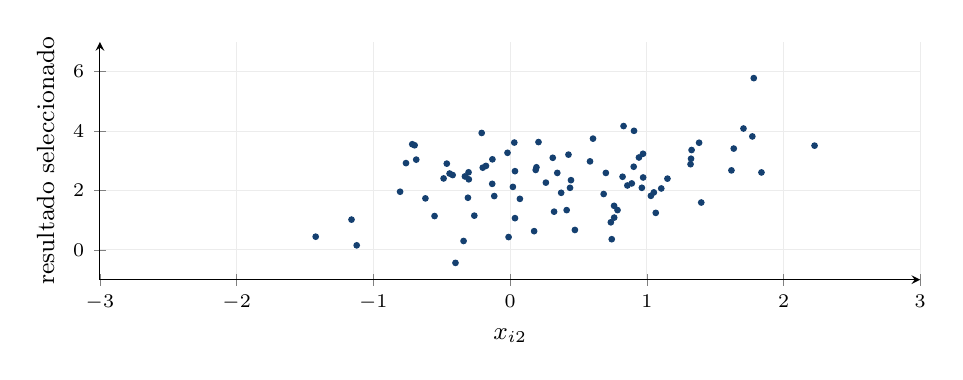
\begin{tikzpicture}\begin{axis}[base,width=12cm,height=4.6cm,xmin=-3,xmax=3,ymin=-1,ymax=7,xlabel={$x_{i2}$},ylabel={resultado seleccionado}]
\addplot[only marks,mark=*,mark size=1pt,azul] coordinates {(0.76139,1.08865) (0.82286,2.46351) (0.85788,2.16931) (-0.01877,3.26953) (0.89001,2.23872) (0.94244,3.11205) (0.96385,2.09110) (0.19289,2.78217) (-0.39928,-0.43611) (-0.46284,2.90491) (-0.71563,3.55829) (1.83861,2.60852) (-0.61933,1.73515) (0.76067,1.48440) (1.32357,3.06975) (-0.41992,2.52065) (0.83007,4.16939) (-0.48621,2.40676) (0.37363,1.92286) (0.42712,3.20812) (2.22694,3.51095) (-0.44240,2.57208) (0.68441,1.88212) (-0.19983,2.76882) (0.07173,1.71954) (-1.42178,0.44589) (-0.55243,1.14031) (0.97322,2.43861) (-0.34004,0.30112) (-0.69817,3.52277) (-1.12178,0.15494) (0.03087,3.61436) (0.03590,1.07014) (0.03581,2.65175) (-0.13074,2.22432) (0.26184,2.26550) (1.31987,2.88571) (1.06550,1.24746) (0.74353,0.36081) (-0.30203,2.37667) (0.20789,3.63058) (0.18744,2.69268) (0.34528,2.59287) (0.90410,2.80059) (0.32190,1.28794) (-0.20769,3.93773) (0.58466,2.98069) (0.90649,4.00907) (1.32760,3.36350) (-0.30828,1.75688) (-0.26148,1.15446) (1.39823,1.59608) (0.73702,0.93004) (0.70055,2.59215) (0.44545,2.34870) (1.77188,3.82061) (0.60650,3.74673) (-0.12924,3.04965) (1.70704,4.08701) (1.61904,2.67768) (-0.76133,2.92259) (1.02991,1.82136) (-0.17640,2.82840) (-1.15977,1.02057) (1.15092,2.40012) (1.63582,3.41211) (1.38253,3.60847) (0.78571,1.34089) (0.43844,2.09043) (-0.11577,1.81271) (1.10575,2.06933) (1.05147,1.93634) (-0.33037,2.47433) (-0.30372,2.61312) (0.41382,1.33983) (1.78232,5.78340) (-0.01095,0.43320) (-0.68635,3.03914) (0.47398,0.67228) (0.97231,3.23667) (0.31220,3.10151) (0.02048,2.12231) (0.17589,0.63203) (-0.80443,1.95914)};
\end{axis}\end{tikzpicture}
\caption{Resultados seleccionados de una muestra artificial; se dibuja una submuestra para legibilidad.}
\end{figure}

\clearpage
\section{Heckman simulado: comparar dos etapas y ajuste conjunto}\label{unidad166}
El probit marginal sobre todos
los indicadores produce
\[
\widehat\gamma_{\mathrm{dos\ etapas}}=\begin{pmatrix}0.2129404\\0.7747328\\0.7803294\end{pmatrix}.
\]

La regresión seleccionada con
la razón normal estimada da
\[
\begin{pmatrix}\widehat\beta_1\\\widehat\beta_2\\\widehat\delta\end{pmatrix}_{\mathrm{dos\ etapas}}=\begin{pmatrix}1.9614107\\0.6479937\\0.6889393\end{pmatrix}.
\]

La reconstrucción de escala
y correlación de momentos produce
\[
1.16910727,\qquad 0.58928664.
\]

El ajuste conjunto se hizo
con coeficientes originales,
log escala y correlación transformada.
Se probaron tres puntos iniciales;
las soluciones convergieron al
mismo objetivo regular en
esta realización.
La raíz final es
\begin{center}\small\begin{tabular}{rrr}\toprule
parámetro&verdadero&estimado conjunto\\\midrule
\(\beta_1\)&2.0000000&1.8924882\\
\(\beta_2\)&0.6000000&0.6777903\\
\(\gamma_1\)&0.2000000&0.2242176\\
\(\gamma_2\)&0.7000000&0.7882224\\
\(\gamma_3\)&0.8000000&0.7817999\\
\(\sigma\)&1.2000000&1.1959147\\
\(\rho\)&0.5500000&0.6718738\\\bottomrule\end{tabular}\end{center}
La diferencia entre procedimientos
en una realización no prueba
sesgo general de uno de ellos.
Ambos están dirigidos a los
parámetros del modelo normal
bajo condiciones correspondientes.

La log-verosimilitud conjunta
en la raíz es
\[
-784.5674405894.
\]

Las siete ecuaciones de score
tienen residuos absolutos menores
que \(10^{-7}\).
La información local tiene
autovalores positivos.
Se reporta una solución
numérica regular verificada,
sin atribuir unicidad global
a todas las muestras posibles
del modelo no lineal.

\clearpage
\section{Heckman simulado: covarianza de los siete parámetros conjuntos}\label{unidad167}
La matriz de información transformada
se obtiene derivando los siete
scores en la raíz.
Se verifica simetría y
positividad local antes de invertir.
El Jacobiano de reconstrucción
de escala y correlación conserva
sus factores \(\sigma\) y \(1-\rho^2\).

En el orden
\[
(\beta_1,\beta_2,\gamma_1,\gamma_2,\gamma_3,\sigma,\rho),
\]
la covarianza local de
parámetros originales es
\[
\begin{pmatrix}0.014985&-0.006712&0.000859&0.000281&0.002400&-0.005417&-0.011192\\-0.006712&0.007567&-0.000131&0.001320&-0.001160&0.002571&0.005259\\0.000859&-0.000131&0.003709&0.000294&0.000618&0.000038&0.000818\\0.000281&0.001320&0.000294&0.005334&0.001621&-0.000460&-0.000450\\0.002400&-0.001160&0.000618&0.001621&0.005486&-0.001266&-0.002079\\-0.005417&0.002571&0.000038&-0.000460&-0.001266&0.004216&0.005066\\-0.011192&0.005259&0.000818&-0.000450&-0.002079&0.005066&0.012274\end{pmatrix}.
\]

Sus errores estándar son
\begin{center}\small\begin{tabular}{rrrr}\toprule
parámetro&error estándar&límite inferior de Wald&límite superior de Wald\\\midrule
\(\beta_1\)&0.1224144&1.6525604&2.1324160\\
\(\beta_2\)&0.0869865&0.5072999&0.8482806\\
\(\gamma_1\)&0.0608983&0.1048591&0.3435761\\
\(\gamma_2\)&0.0730357&0.6450751&0.9313697\\
\(\gamma_3\)&0.0740694&0.6366265&0.9269734\\
\(\sigma\)&0.0649275&1.0686592&1.3231702\\
\(\rho\)&0.1107859&0.4547374&0.8890103\\\bottomrule\end{tabular}\end{center}
Estos son intervalos de primer orden.
Para escala y correlación puede
preferirse transformar intervalos
de las coordenadas no restringidas,
preservando positividad y
el rango interior de correlación.

Los cruces entre selección,
resultado y escala no se
omitieron. La covarianza de
\(\delta=\rho\sigma\) utiliza
la combinación de las
últimas dos coordenadas.
Su varianza aproximada es
\[
0.027597664.
\]

La matriz corresponde al
mecanismo normal conjunto correcto
y a esta realización simulada.
No representa una covarianza
exacta finita ni una
tabla estimada con una
base empírica no proporcionada.

\clearpage
\addcontentsline{toc}{part}{Problemas integrados, efectos fijos y curiosidades matemáticas}
\pdfbookmark[0]{Problemas integrados, efectos fijos y curiosidades matemáticas}{parte168}
\section{Problema integrado RD: curvatura, sesgo finito y corrección}\label{unidad168}
Mantengamos los dieciséis puntajes y
el kernel del laboratorio.
Las medias verdaderas son ahora
\[
\begin{aligned}
\text{izquierda}:&\quad2+.5x_{i2}+.3x_{i2}^2,\\
\text{derecha}:&\quad5+x_{i2}+.8x_{i2}^2.
\end{aligned}
\]
El salto verdadero sigue siendo tres.
La diferencia de segundas derivadas
es \(1.6-.6=1\).
Ajustar rectas a esos valores
de media produce
\[
\E[\widehat\beta_{\mathrm{lineal}}\mid X]
=\begin{pmatrix}1.3250000\\1.8750000\\-0.5500000\\4.3500000\end{pmatrix}.
\]

El sesgo finito del salto es
\[
1.87500000-3=-1.12500000.
\]

Una cuadrática local añade columnas
\(x_{i2}^2,D_ix_{i2}^2\).
Su solución sobre estas medias es
\[
\begin{pmatrix}2.0000000\\3.0000000\\0.5000000\\0.5000000\\0.3000000\\0.5000000\end{pmatrix}.
\]

El coeficiente de interacción cuadrática
es .5. Dos veces ese coeficiente
recupera la diferencia de curvaturas uno.

El coeficiente finito de curvatura
en el intercepto derecho de una recta
es la suma de sus pesos
por \(x_{i2}^2\):
\[
-2.2500000000.
\]

Con este diseño simétrico,
el izquierdo tiene el mismo coeficiente.
La corrección finita resta
esa cantidad por .5
al salto lineal:
\[
1.87500000-(-2.25000000)(.5)=3.00000000.
\]

Se recupera exactamente tres
para estas medias cuadráticas.
La constante asintótica \(-h^2/20\)
por curvatura diferencial no
se confundió con el coeficiente
exacto de esta muestra de puntajes.

\begin{figure}[H]\centering
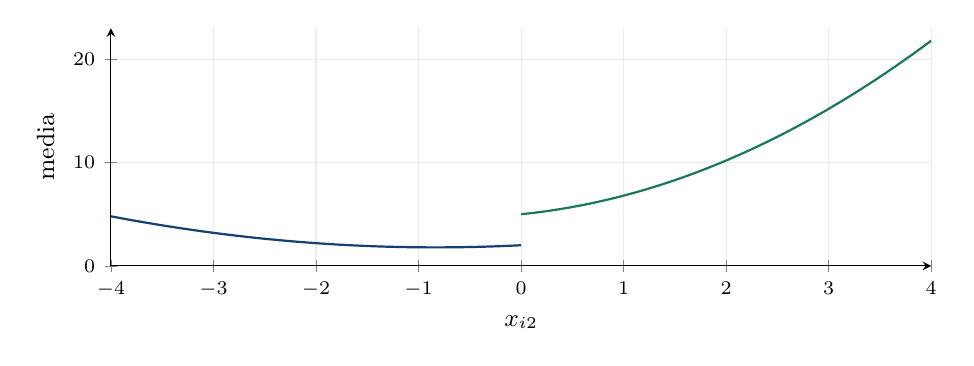
\begin{tikzpicture}\begin{axis}[base,width=12cm,height=4.6cm,xmin=-4,xmax=4,ymin=0,ymax=23,xlabel={$x_{i2}$},ylabel={media}]
\addplot[azul,thick,domain=-4:0]{2+.5*x+.3*x^2};\addplot[verde,thick,domain=0:4]{5+x+.8*x^2};
\end{axis}\end{tikzpicture}
\caption{Medias curvas con salto tres; una recta local puede extrapolar un salto distinto.}
\end{figure}

\clearpage
\section{Problema integrado RD: covarianza de la corrección de curvatura}\label{unidad169}
El ajuste cuadrático utiliza seis
columnas y tiene producto cruzado
\[
\begin{pmatrix}7.00000&3.50000&0&5.25000&21.00000&10.50000\\3.50000&3.50000&5.25000&5.25000&10.50000&10.50000\\0&5.25000&21.00000&10.50000&0&24.93750\\5.25000&5.25000&10.50000&10.50000&24.93750&24.93750\\21.00000&10.50000&0&24.93750&131.25000&65.62500\\10.50000&10.50000&24.93750&24.93750&65.62500&65.62500\end{pmatrix}.
\]

Con errores independientes de varianza .25,
su covarianza condicionada es
\[
\begin{pmatrix}0.676020&-0.676020&0.750000&-0.750000&0.173469&-0.173469\\-0.676020&1.352041&-0.750000&0&-0.173469&0.346939\\0.750000&-0.750000&0.964286&-0.964286&0.238095&-0.238095\\-0.750000&0&-0.964286&1.928571&-0.238095&0\\0.173469&-0.173469&0.238095&-0.238095&0.061224&-0.061224\\-0.173469&0.346939&-0.238095&0&-0.061224&0.122449\end{pmatrix}.
\]

La diferencia estimada de curvaturas
es dos veces su sexta coordenada.
Su varianza y la covarianza con
el salto lineal se calculan
propagando ambas transformaciones
sobre las mismas respuestas.

Los valores son
\[
\begin{aligned}
\Var(\widehat\tau_{\mathrm{lineal}})&=0.410714286,\\
\Var(\text{diferencia de curvaturas})&=0.489795918,\\
\Cov(\widehat\tau_{\mathrm{lineal}},
\text{diferencia de curvaturas})&=0.142857143.\end{aligned}
\]

La corrección resta la diferencia
de curvaturas por la mitad del
coeficiente finito de extrapolación.
La propagación completa es
\[
\begin{aligned}
&0.410714286+\left(-1.125000000\right)^2(0.489795918)\\
&\qquad-2(-1.125000000)(0.142857143)
=1.352040816.\end{aligned}
\]

También se verifica sumando
los cuadrados de todos
los pesos corregidos por .25.
El cálculo coincide con
la varianza del salto cuadrático
para este diseño y
corrección finita equivalentes.

Las respuestas usadas antes eran
las medias verdaderas,
para estudiar sesgo sin
una realización de ruido.
La covarianza de esta unidad
se refiere al mecanismo
con errores de varianza conocida,
no a residuos cero
tomados como varianza cero.

Corregir el centro del estimador
y corregir su incertidumbre
son operaciones que deben
hacerse conjuntamente.

\clearpage
\section{Problema de efectos fijos: la censura no desaparece al centrar}\label{unidad170}
Consideremos dos tiempos y
la misma parte regresora
\((-1,1)\) en dos individuos.
El primer intercepto es cero
y el segundo es dos.
Sin errores, sus latentes son
\[
(-1,1)\quad\text{y}\quad(1,3).
\]
Tras censura en cero,
los observados son
\[
(0,1)\quad\text{y}\quad(1,3).
\]
Las medias observadas son .5 y dos.
Al restarlas dentro de individuo,
se obtiene
\[
(-.5,.5)\quad\text{y}\quad(-1,1).
\]
Aunque la parte regresora
original es la misma,
los observados centrados
son distintos por sus interceptos.

En un modelo lineal sin
censura, centrar habría
eliminado ambos interceptos,
dejando la misma parte
\((-1,1)\).
Aquí no se eliminó
su efecto sobre cuáles
valores se acumulan en cero.

La identidad que falla es
\[
\begin{aligned}
&\max(0,\alpha_i+x_{it}\T\beta)
-\frac1T\sum_s\max(0,\alpha_i+x_{is}\T\beta)\\
&\ne x_{it}\T\beta-\frac1T\sum_sx_{is}\T\beta
\end{aligned}
\]
en general.
La función máximo es no lineal
y cambia la forma de
dependencia de cada respuesta
en el intercepto.

\begin{ejemplo}[Qué sigue siendo exacto]
Centrar los latentes lineales sí
elimina \(\alpha_i\).
El problema es que
los latentes censurados no
se observan, por lo que
esa transformación no está
disponible en los datos.
\end{ejemplo}
Este ejemplo no demuestra
que nunca se pueda
estimar un panel censurado.
Demuestra que el procedimiento
lineal within no se
traslada automáticamente al Tobit.

Un modelo de panel
censurado necesita discutir
cómo se tratan sus
interceptos, su número
y la distribución conjunta
de errores en el tiempo.

\clearpage
\section{Problema de parámetros incidentales: muchos interceptos con dos observaciones}\label{unidad171}
Considérese
\(Y_{it}=\alpha_i+\varepsilon_{it}\),
\(t=1,2\), con errores
normales independientes de
varianza \(\sigma^2\).
El máximo de cada intercepto es
\[
\widehat\alpha_i=(Y_{i1}+Y_{i2})/2.
\]
Sus dos residuos son
\((Y_{i1}-Y_{i2})/2\)
y su opuesto.
La suma de cuadrados
dentro del individuo es
\[
(Y_{i1}-Y_{i2})^2/2.
\]

El máximo normal de
varianza divide la suma
de todos los residuos
por \(2N\):
\[
\widehat\sigma^2_{\mathrm{MV}}
=\frac1{4N}\sum_{i=1}^N(Y_{i1}-Y_{i2})^2.
\]
La diferencia elimina
el intercepto y tiene
varianza \(2\sigma^2\).
Su esperanza cuadrada es
\(2\sigma^2\).
Por tanto,
\[
\E[\widehat\sigma^2_{\mathrm{MV}}]
=\sigma^2/2.
\]
Una ley de grandes números
también lleva el estimador
hacia \(\sigma^2/2\)
al crecer \(N\) con
dos tiempos fijos.

El número de interceptos
crece junto con la muestra,
pero cada uno utiliza
solo dos observaciones.
La inconsistencia persiste,
a diferencia de un
modelo de dimensión fija.

\begin{ejemplo}[Corrección en este modelo]
Duplicar esta regla de
varianza recupera una
estimación consistente.
Esa corrección se dedujo
para el ejemplo normal;
no se transporta como
factor universal a Tobit
o selección no lineal.
\end{ejemplo}
Los paneles no lineales
con efectos individuales
pueden tener problemas
de parámetros incidentales.
La presencia de muchos
registros totales no
garantiza la misma precisión
por cada intercepto.

El ejemplo muestra un
mecanismo matemático concreto.
No afirma que toda
pendiente de un modelo
lineal within sea
inconsistente por usar
muchos efectos fijos.

\clearpage
\section{Selección y efectos fijos: centrar también la corrección}\label{unidad172}
Supongamos una ecuación seleccionada
con intercepto individual:
\[
Y_{it}^\ast=\alpha_i+\sum_jx_{itj}\beta_j
+\delta\frac{\varphi(\sum_lz_{itl}\gamma_l)}
{\Phi(\sum_lz_{itl}\gamma_l)}
+\text{error seleccionado centrado}.
\]
Para los tiempos observados,
restar su media elimina
\(\alpha_i\), pero también
centra la columna de Mills.

Si hay \(m_i\) tiempos seleccionados,
el término de corrección que queda es
\[
\begin{aligned}
\delta\Bigg[
&\frac{\varphi(\sum_lz_{itl}\gamma_l)}
{\Phi(\sum_lz_{itl}\gamma_l)}\\
&-\frac1{m_i}\sum_{s:S_{is}=1}
\frac{\varphi(\sum_lz_{isl}\gamma_l)}
{\Phi(\sum_lz_{isl}\gamma_l)}
\Bigg].
\end{aligned}
\]
Los regresores se transforman
restando sus medias sobre
esos mismos tiempos seleccionados.
No se conserva intacta
una razón sin centrar
al lado de datos centrados.

El número \(m_i\) depende
del patrón de selección.
Con un solo tiempo observado,
toda la variación within
de ese individuo es cero.
Con razones constantes
en sus tiempos seleccionados,
la corrección también pierde
variación within.

\begin{ejemplo}[Dos razones distintas]
Si las razones son .4 y .8,
su media es .6
y sus valores centrados
son \(-.2,.2\).
Omitir esta transformación
cambia la ecuación.
\end{ejemplo}
La identidad es algebraica
para una media seleccionada
correctamente especificada.
Un modelo de panel completo
necesita además especificar
dependencia temporal y
efectos en la selección.

El Heckman transversal básico
no se convierte automáticamente
en un estimador de
panel válido por añadir
dummies individuales.
Hay que volver a
analizar identificación,
regresores generados y
covarianzas entre tiempos.

\clearpage
\section{Ecuación Mincer y selección: qué muestra pertenece a cada etapa}\label{unidad173}
Una ecuación de ingreso por hora
puede utilizar como resultado
su logaritmo y una media
de tipo Mincer:
\[
\begin{aligned}
Y_i^\ast={}&\beta_1+\beta_2x_{i2}
+\beta_3x_{i3}+\beta_4x_{i3}^2\\
&+\sum_{j=5}^kx_{ij}\beta_j+\varepsilon_i.
\end{aligned}
\]
Por ejemplo, \(x_{i2}\)
puede medir educación y
\(x_{i3}\) experiencia.
Las demás columnas deben
definirse según la pregunta
y la población del estudio.

La selección no es
tener salario igual a cero:
puede representar que
ingreso y horas válidos
están disponibles.
El probit se estima
sobre la población elegible,
incluyendo indicadores cero
de ausencia de resultado.

La segunda etapa utiliza
solo quienes tienen
el resultado logarítmico válido:
\[
Y_i=\sum_jx_{ij}\beta_j+
\delta\frac{\varphi(\sum_lz_{il}\widehat\gamma_l)}
{\Phi(\sum_lz_{il}\widehat\gamma_l)}
+\text{error centrado},\qquad S_i=1.
\]
El uso de logaritmos
debe corresponder a
ingresos positivos observables;
no se toma logaritmo
de una ausencia de salario.

\begin{ejemplo}[Efecto marginal de experiencia]
La derivada de la
media potencial respecto
de experiencia es
\(\beta_3+2\beta_4x_{i3}\).
La media seleccionada
puede añadir también
un cambio de su razón
si experiencia participa
en la ecuación de selección.
\end{ejemplo}
Dummies de año y mes
pueden describir cambios
de media temporal.
Su inclusión no sustituye
el mecanismo de selección,
ni prueba exogeneidad
de los regresores de ingreso.

Este es un ejemplo
de especificación matemática.
No se han estimado
resultados con una base
empírica de ingresos
no proporcionada en esta tarea.

\clearpage
\section{Curiosidad Tobit: la media censurada es convexa aunque el latente sea lineal}\label{unidad174}
La media observada a escala uno,
como función de su producto latente,
es
\[
\left(\sum_jx_{ij}\beta_j\right)
\Phi\left(\sum_jx_{ij}\beta_j\right)
+\varphi\left(\sum_jx_{ij}\beta_j\right).
\]
Su primera derivada respecto
de ese producto es
la acumulada normal.
Su segunda derivada es
la densidad normal,
estrictamente positiva.

Por ello la media observada
es una función convexa
del producto latente.
Una recta de coeficientes
latentes no produce una
recta de medias observadas
bajo censura.

Además, \(Y_i\ge Y_i^\ast\)
y \(Y_i\ge0\) en
cada realización.
Tomar esperanza muestra
\[
\E[Y_i\mid x_i]\ge
\max\left(0,\sum_jx_{ij}\beta_j\right).
\]
La desigualdad se obtuvo
directamente de dos
comparaciones punto a punto,
sin reemplazar una
esperanza de función
por una función de esperanza.


\begin{figure}[H]\centering
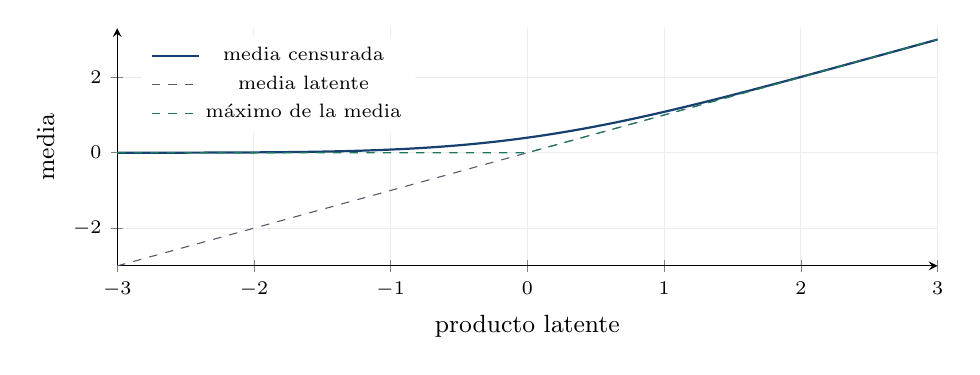
\begin{tikzpicture}\begin{axis}[base,width=12cm,height=4.6cm,xmin=-3,xmax=3,ymin=-3,ymax=3.3,xlabel={producto latente},ylabel={media},legend pos=north west]
\addplot[azul,thick] coordinates {(-3.000000,0.000382154) (-2.939394,0.000472619) (-2.878788,0.000582619) (-2.818182,0.000715916) (-2.757576,0.000876899) (-2.696970,0.001070660) (-2.636364,0.001303086) (-2.575758,0.001580955) (-2.515152,0.001912038) (-2.454545,0.002305205) (-2.393939,0.002770539) (-2.333333,0.003319456) (-2.272727,0.003964818) (-2.212121,0.004721065) (-2.151515,0.005604326) (-2.090909,0.006632546) (-2.030303,0.007825599) (-1.969697,0.009205396) (-1.909091,0.010795987) (-1.848485,0.012623646) (-1.787879,0.014716945) (-1.727273,0.017106809) (-1.666667,0.019826552) (-1.606061,0.022911882) (-1.545455,0.026400890) (-1.484848,0.030334004) (-1.424242,0.034753907) (-1.363636,0.039705432) (-1.303030,0.045235413) (-1.242424,0.051392503) (-1.181818,0.058226957) (-1.121212,0.065790376) (-1.060606,0.074135417) (-1.000000,0.083315471) (-0.939394,0.093384305) (-0.878788,0.104395686) (-0.818182,0.116402968) (-0.757576,0.129458669) (-0.696970,0.143614035) (-0.636364,0.158918588) (-0.575758,0.175419682) (-0.515152,0.193162055) (-0.454545,0.212187402) (-0.393939,0.232533959) (-0.333333,0.254236114) (-0.272727,0.277324057) (-0.212121,0.301823457) (-0.151515,0.327755192) (-0.090909,0.355135122) (-0.030303,0.383973920) (0.030303,0.414276951) (0.090909,0.446044213) (0.151515,0.479270343) (0.212121,0.513944669) (0.272727,0.550051330) (0.333333,0.587569448) (0.393939,0.626473353) (0.454545,0.666732857) (0.515152,0.708313570) (0.575758,0.751177257) (0.636364,0.795282224) (0.696970,0.840583732) (0.757576,0.887034427) (0.818182,0.934584786) (0.878788,0.983183565) (0.939394,1.032778245) (1.000000,1.083315471) (1.060606,1.134741478) (1.121212,1.187002497) (1.181818,1.240045139) (1.242424,1.293816746) (1.303030,1.348265716) (1.363636,1.403341796) (1.424242,1.458996331) (1.484848,1.515182488) (1.545455,1.571855436) (1.606061,1.628972488) (1.666667,1.686493218) (1.727273,1.744379537) (1.787879,1.802595733) (1.848485,1.861108495) (1.909091,1.919886896) (1.969697,1.978902366) (2.030303,2.038128629) (2.090909,2.097541637) (2.151515,2.157119477) (2.212121,2.216842277) (2.272727,2.276692091) (2.333333,2.336652789) (2.393939,2.396709933) (2.454545,2.456850659) (2.515152,2.517063553) (2.575758,2.577338531) (2.636364,2.637666722) (2.696970,2.698040356) (2.757576,2.758452656) (2.818182,2.818897734) (2.878788,2.879370498) (2.939394,2.939866559) (3.000000,3.000382154)};\addplot[gris,dashed,domain=-3:3]{x};\addplot[verde,dashed,domain=-3:3]{max(0,x)};\legend{media censurada,media latente,máximo de la media}
\end{axis}\end{tikzpicture}
\caption{Media observada censurada, media latente y máximo de cero con la media latente.}
\end{figure}

El máximo de la media
tiene un quiebre en cero.
La esperanza de la
respuesta censurada es suave:
integra una distribución
de errores alrededor
del límite.

La diferencia es mayor
cerca del punto donde
la censura tiene probabilidad
intermedia. En colas positivas,
la media se aproxima
a la lineal latente.
En colas negativas,
se aproxima a cero.

\clearpage
\section{Curiosidad Heckman: visualizar la selección dentro de una normal bivariada}\label{unidad175}
Usemos errores estandarizados de
correlación .6 y un
índice de selección cero.
La selección conserva
\(\nu_i>0\).
Una curva de nivel
de densidad conjunta
puede parametrizarse como
\[
\begin{aligned}
\nu_i&=2\sin\theta,\\
\varepsilon_i/\sigma
&=2[.6\sin\theta+.8\cos\theta].
\end{aligned}
\]
Sustituir verifica
\[
\nu_i^2+\frac{(\varepsilon_i/\sigma-.6\nu_i)^2}{.8^2}=4.
\]
La escala igual de
ambos ejes conserva
la geometría de esa elipse.

La media original de
ambos errores es cero.
Entre seleccionados,
\[
\E[\nu_i\mid S_i=1]=\sqrt{2/\pi},
\quad
\E[\varepsilon_i/\sigma\mid S_i=1]
=.6\sqrt{2/\pi}.
\]
Ambas coordenadas se
desplazan al condicionar
en la mitad superior.


\begin{figure}[H]\centering
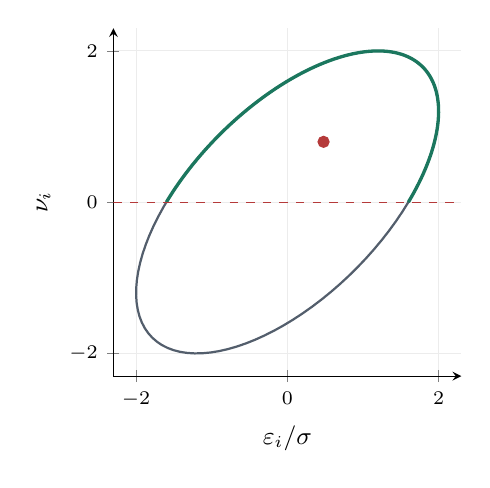
\begin{tikzpicture}\begin{axis}[base,width=12cm,height=6cm,axis equal image,xmin=-2.3,xmax=2.3,ymin=-2.3,ymax=2.3,xlabel={$\varepsilon_i/\sigma$},ylabel={$\nu_i$}]
\addplot[gris,thick,domain=0:360,variable=\t] ({2*(.6*sin(\t)+.8*cos(\t))},{2*sin(\t)});\addplot[verde,very thick,domain=0:180,variable=\t] ({2*(.6*sin(\t)+.8*cos(\t))},{2*sin(\t)});\addplot[rojo,dashed] coordinates {(-2.3,0)(2.3,0)};\addplot[rojo,only marks,mark=*] coordinates {(.478730736,.797884561)};
\end{axis}\end{tikzpicture}
\caption{Elipse de nivel de densidad original, frontera de selección y desplazamiento de media.}
\end{figure}

La curva no es una
elipse de confianza de
un estimador.
Es un nivel de
densidad de dos errores
y una región de selección.

Cortar la normal conjunta
cambia la composición
del error de resultado
si ambos están correlacionados.
Esta imagen corresponde
a la integral que
produjo Mills y a
la corrección de media,
no a una relación
causal automática entre errores.

\clearpage
\section{Curiosidad Mills: media condicionada y varianza se mueven de forma distinta}\label{unidad176}
Para el evento \(\nu_i>-\sum_lz_{il}\gamma_l\),
la media del error
es una razón normal,
mientras su varianza
es uno más la
derivada de esa razón.
La primera función
disminuye con el índice;
la varianza pasa desde
valores pequeños en
selección de cola alta
hasta valores cercanos a uno.

Las dos gráficas evalúan
argumentos escalares
entre menos cuatro y cuatro.
Al aplicarlas a una fila,
el argumento se reemplaza
por su suma de
regresores de selección.

\begin{figure}[H]\centering
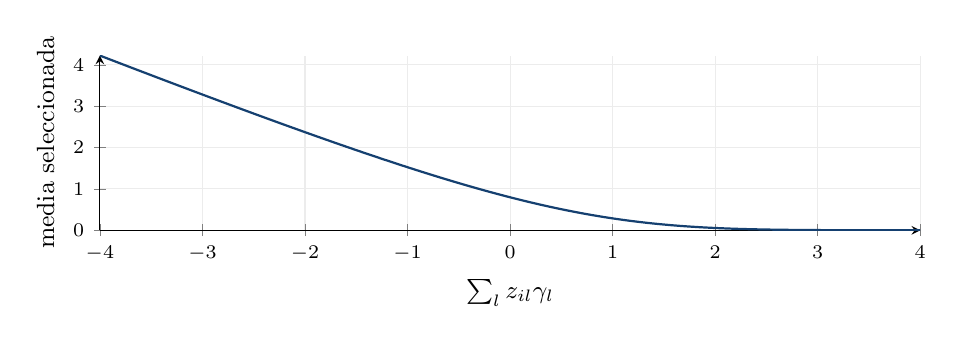
\begin{tikzpicture}\begin{axis}[base,width=12cm,height=3.8cm,xmin=-4,xmax=4,ymin=0,xlabel={$\sum_lz_{il}\gamma_l$},ylabel={media seleccionada}]
\addplot[azul,thick] coordinates {(-4.000000,4.225607144) (-3.919192,4.148629754) (-3.838384,4.071774140) (-3.757576,3.995045741) (-3.676768,3.918450296) (-3.595960,3.841993864) (-3.515152,3.765682849) (-3.434343,3.689524014) (-3.353535,3.613524512) (-3.272727,3.537691908) (-3.191919,3.462034206) (-3.111111,3.386559877) (-3.030303,3.311277890) (-2.949495,3.236197747) (-2.868687,3.161329514) (-2.787879,3.086683859) (-2.707071,3.012272096) (-2.626263,2.938106219) (-2.545455,2.864198953) (-2.464646,2.790563799) (-2.383838,2.717215085) (-2.303030,2.644168018) (-2.222222,2.571438739) (-2.141414,2.499044386) (-2.060606,2.427003151) (-1.979798,2.355334348) (-1.898990,2.284058480) (-1.818182,2.213197309) (-1.737374,2.142773927) (-1.656566,2.072812835) (-1.575758,2.003340015) (-1.494949,1.934383009) (-1.414141,1.865970996) (-1.333333,1.798134869) (-1.252525,1.730907311) (-1.171717,1.664322862) (-1.090909,1.598417990) (-1.010101,1.533231150) (-0.929293,1.468802832) (-0.848485,1.405175598) (-0.767677,1.342394108) (-0.686869,1.280505122) (-0.606061,1.219557480) (-0.525253,1.159602057) (-0.444444,1.100691685) (-0.363636,1.042881037) (-0.282828,0.986226467) (-0.202020,0.930785803) (-0.121212,0.876618090) (-0.040404,0.823783262) (0.040404,0.772341763) (0.121212,0.722354088) (0.202020,0.673880260) (0.282828,0.626979227) (0.363636,0.581708192) (0.444444,0.538121875) (0.525253,0.496271705) (0.606061,0.456204968) (0.686869,0.417963915) (0.767677,0.381584849) (0.848485,0.347097214) (0.929293,0.314522719) (1.010101,0.283874514) (1.090909,0.255156467) (1.171717,0.228362551) (1.252525,0.203476404) (1.333333,0.180471060) (1.414141,0.159308908) (1.494949,0.139941863) (1.575758,0.122311794) (1.656566,0.106351180) (1.737374,0.091984004) (1.818182,0.079126844) (1.898990,0.067690150) (1.979798,0.057579648) (2.060606,0.048697828) (2.141414,0.040945469) (2.222222,0.034223143) (2.303030,0.028432647) (2.383838,0.023478321) (2.464646,0.019268212) (2.545455,0.015715053) (2.626263,0.012737047) (2.707071,0.010258438) (2.787879,0.008209885) (2.868687,0.006528633) (2.949495,0.005158518) (3.030303,0.004049813) (3.111111,0.003158960) (3.191919,0.002448191) (3.272727,0.001885094) (3.353535,0.001442123) (3.434343,0.001096098) (3.515152,0.000827697) (3.595960,0.000620963) (3.676768,0.000462839) (3.757576,0.000342739) (3.838384,0.000252154) (3.919192,0.000184303) (4.000000,0.000133834)};
\end{axis}\end{tikzpicture}
\caption{Media del error seleccionado como función del índice.}
\end{figure}

\begin{figure}[H]\centering
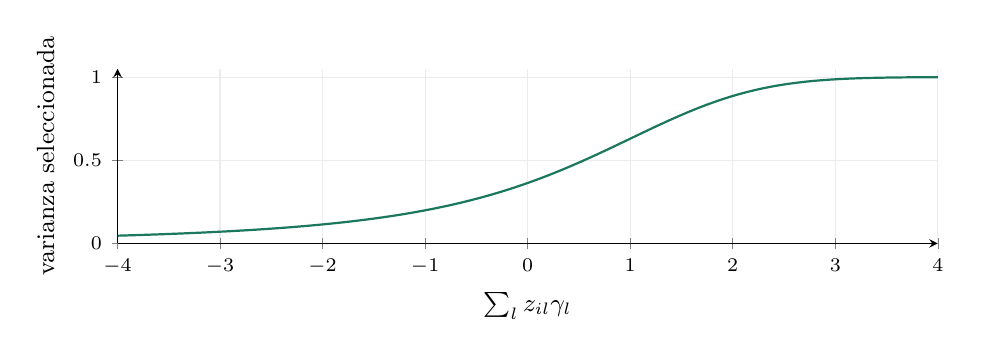
\begin{tikzpicture}\begin{axis}[base,width=12cm,height=3.8cm,xmin=-4,xmax=4,ymin=0,ymax=1.05,xlabel={$\sum_lz_{il}\gamma_l$},ylabel={varianza seleccionada}]
\addplot[verde,thick] coordinates {(-4.000000,0.046672838) (-3.919192,0.048147372) (-3.838384,0.049687404) (-3.757576,0.051296553) (-3.676768,0.052978669) (-3.595960,0.054737850) (-3.515152,0.056578455) (-3.434343,0.058505125) (-3.353535,0.060522804) (-3.272727,0.062636754) (-3.191919,0.064852582) (-3.111111,0.067176263) (-3.030303,0.069614159) (-2.949495,0.072173053) (-2.868687,0.074860170) (-2.787879,0.077683209) (-2.707071,0.080650373) (-2.626263,0.083770402) (-2.545455,0.087052603) (-2.464646,0.090506885) (-2.383838,0.094143798) (-2.303030,0.097974565) (-2.222222,0.102011120) (-2.141414,0.106266145) (-2.060606,0.110753108) (-1.979798,0.115486293) (-1.898990,0.120480842) (-1.818182,0.125752780) (-1.737374,0.131319044) (-1.656566,0.137197506) (-1.575758,0.143406989) (-1.494949,0.149967277) (-1.414141,0.156899105) (-1.333333,0.164224150) (-1.252525,0.171964998) (-1.171717,0.180145089) (-1.090909,0.188788645) (-1.010101,0.197920573) (-0.929293,0.207566327) (-0.848485,0.217751743) (-0.767677,0.228502828) (-0.686869,0.239845504) (-0.606061,0.251805299) (-0.525253,0.264406978) (-0.444444,0.277674118) (-0.363636,0.291628610) (-0.282828,0.306290095) (-0.202020,0.321675325) (-0.121212,0.337797463) (-0.040404,0.354665310) (0.040404,0.372282473) (0.121212,0.390646500) (0.202020,0.409747969) (0.282828,0.429569591) (0.363636,0.450085327) (0.444444,0.471259570) (0.525253,0.493046429) (0.606061,0.515389168) (0.686869,0.538219840) (0.767677,0.561459180) (0.848485,0.585016797) (0.929293,0.608791721) (1.010101,0.632673326) (1.090909,0.656542668) (1.171717,0.680274222) (1.252525,0.703738019) (1.333333,0.726802116) (1.414141,0.749335348) (1.494949,0.771210258) (1.575758,0.792306090) (1.656566,0.812511714) (1.737374,0.831728350) (1.818182,0.849871954) (1.898990,0.866875132) (1.979798,0.882688513) (2.060606,0.897281482) (2.141414,0.910642262) (2.222222,0.922777348) (2.303030,0.933710337) (2.383838,0.943480245) (2.464646,0.952139405) (2.545455,0.959751084) (2.626263,0.966386938) (2.707071,0.972124447) (2.787879,0.977044433) (2.868687,0.981228773) (2.949495,0.984758368) (3.030303,0.987711437) (3.111111,0.990162145) (3.191919,0.992179577) (3.272727,0.993827049) (3.353535,0.995161711) (3.434343,0.996234422) (3.515152,0.997089836) (3.595960,0.997766658) (3.676768,0.998298033) (3.757576,0.998712014) (3.838384,0.999032074) (3.919192,0.999277645) (4.000000,0.999464644)};
\end{axis}\end{tikzpicture}
\caption{Varianza del mismo error estandarizado condicionado en selección.}
\end{figure}

Una media seleccionada alta
no implica gran dispersión
alrededor de esa media.
En una cola rara,
los errores conservados
están concentrados cerca
de un umbral alto.

En Heckman, una parte
normal independiente del
error de selección permanece.
Por eso su varianza
de resultado no tiene
que acercarse a cero
aunque la del
error truncado sí
se vuelva pequeña.

\clearpage
\section{Problema avanzado: desplegar la varianza heredada de la selección}\label{unidad177}
En el modelo correcto, las perturbaciones originales de
momentos de ambas etapas son ortogonales en población.
La sensibilidad poblacional de la segunda etapa respecto
de selección contiene \(\delta\) por una suma de
filas ampliadas, el factor normal de truncamiento y \(z_i\T\).

El término adicional que se suma a la matriz central
de la covarianza de resultados es
\[
\begin{aligned}
\delta^2&
\left[\sum_{S_i=1}
\begin{pmatrix}x_i\\\frac{\varphi(\sum_lz_{il}\gamma_l)}{\Phi(\sum_lz_{il}\gamma_l)}\end{pmatrix}
\frac{\varphi(\sum_lz_{il}\gamma_l)}{\Phi(\sum_lz_{il}\gamma_l)}\left[\sum_lz_{il}\gamma_l+\frac{\varphi(\sum_lz_{il}\gamma_l)}{\Phi(\sum_lz_{il}\gamma_l)}\right]z_i\T\right]\\
&\cdot\left[\sum_{i=1}^n
\frac{\varphi(\sum_lz_{il}\gamma_l)^2}
{\Phi(\sum_lz_{il}\gamma_l)\Phi(-\sum_lz_{il}\gamma_l)}
z_iz_i\T\right]^{-1}\\
&\cdot\left[\sum_{S_r=1}
z_r\frac{\varphi(\sum_lz_{rl}\gamma_l)}
{\Phi(\sum_lz_{rl}\gamma_l)}
\left[\sum_lz_{rl}\gamma_l+
\frac{\varphi(\sum_lz_{rl}\gamma_l)}
{\Phi(\sum_lz_{rl}\gamma_l)}\right]\right.\\
&\qquad\qquad\left.\cdot
\left(x_r\T,\frac{\varphi(\sum_lz_{rl}\gamma_l)}
{\Phi(\sum_lz_{rl}\gamma_l)}\right)\right].
\end{aligned}
\]

El primer y último factores son transpuestos.
La inversa central pertenece al probit de todas las filas,
no solamente de seleccionados.
Por eso la dimensión de esa inversa es \(q\).

Esta matriz es semidefinida positiva.
Para obtener la contribución final a la covarianza
de \((\widehat\beta,\widehat\delta)\),
se multiplica a izquierda y derecha por
\[
\left[\sum_{S_i=1}\begin{pmatrix}x_i\\\frac{\varphi(\sum_lz_{il}\gamma_l)}{\Phi(\sum_lz_{il}\gamma_l)}\end{pmatrix}\left(x_i\T,\ \frac{\varphi(\sum_lz_{il}\gamma_l)}{\Phi(\sum_lz_{il}\gamma_l)}\right)\right]^{-1}.
\]

Se suma a la propagación de la varianza de error
seleccionado de primera etapa conocida.
Si \(\delta=0\), desaparece este término poblacional
de sensibilidad sistemática.

La expresión es una aproximación de primer orden del modelo
correctamente especificado. En un sándwich empírico general,
se conservan además los cruces muestrales y el término de
derivada por residuo de la ecuación de corrección.
Esos componentes se imprimieron en el laboratorio conjunto.

\clearpage
\section{Problema completo FIML: una fila y las siete derivadas}\label{unidad178}
\begin{ejemplo}[Sustituir una fila en el score conjunto]Tomemos \(x_i=(1,0.761389)\T\), \(z_i=(1,0.761389,0.386337)\T\), \(y_i=1.088645\), con \(S_i=1\). En el vector de parámetros \[
\beta=\begin{pmatrix}1.892488\\0.677790\end{pmatrix},\quad\gamma=\begin{pmatrix}0.224218\\0.788222\\0.781800\end{pmatrix},\quad\sigma=1.195915,\quad\rho=0.671874.
\]
Las multiplicaciones de los datos por esos coeficientes dan \[
\sum_jx_{ij}\beta_j=2.40855031,\quad\sum_lz_{il}\gamma_l=1.12639986.
\]
El residuo dividido por escala es \[
\frac{1.08864520-(2.40855031)}{1.19591472}=-1.10367828.
\]
La acumulada condicional usa \[
\frac{(1.12639986)+(0.67187382)(-1.10367828)}{\sqrt{1-(0.67187382)^2}}=0.51962357.
\]
Su razón normal es \[
\frac{\varphi(0.51962357)}{\Phi(0.51962357)}=0.49912965.
\]

La parte normal del score de resultados y su parte de selección
son, por separado,
\[
\begin{pmatrix}-0.92287373\\-0.70266601\end{pmatrix},\qquad\begin{pmatrix}-0.37859832\\-0.28826064\end{pmatrix}.
\]

Sumar esos vectores da las dos primeras coordenadas.
Las tres de selección multiplican la razón normal por
\(z_i/\sqrt{1-\rho^2}\).
La de escala suma el Jacobiano, el residuo cuadrado
y el cambio de la acumulada.
La de correlación incluye la derivada del denominador.

Reunir las siete contribuciones, en el orden
\((\beta_1,\beta_2,\gamma_1,\gamma_2,\gamma_3,\sigma,\rho)\),
produce
\[
\begin{pmatrix}-1.30147205\\-0.99092665\\0.67389336\\0.51309506\\0.26035002\\0.60022642\\-0.42611389\end{pmatrix}.
\]

Los datos y el argumento se mantuvieron idénticos para
todos los componentes. Esta es una contribución de fila;
la raíz conjunta exige que la suma de todos los vectores
por observación sea cero.

Una fila no seleccionada aportaría solamente
sus tres coordenadas de selección, con el cociente
de argumento \(-\sum_lz_{il}\gamma_l\).
Las cuatro coordenadas de resultado, escala y correlación
serían cero porque ese resultado no se observó.
\end{ejemplo}

\clearpage
\addcontentsline{toc}{part}{Referencias y cierre matemático}
\pdfbookmark[0]{Referencias y cierre matemático}{parte179}
\section{Fuentes primarias y condiciones de lectura}\label{unidad179}
Las demostraciones del documento desarrollan
las ecuaciones y los datos explícitos.
Las fuentes primarias siguientes permiten
continuar el estudio de los mecanismos
y de la inferencia no paramétrica.

Los tres problemas no se intercambian.
La discontinuidad necesita hipótesis causales
en el corte. Tobit necesita un
mecanismo de censura. Heckman necesita
un modelo de selección y su
relación con resultados no observados.

Las identidades de momentos condicionados,
los resultados numéricos y los
límites asintóticos se han identificado
por separado. Las covarianzas de
estimadores no se confunden con
las varianzas de respuestas o
errores de una sola observación.

\begin{thebibliography}{9}
\bibitem{tobin1958}
James Tobin. Estimation of Relationships for Limited Dependent Variables.
\emph{Econometrica}, 26(1), 24--36, 1958.
\url{https://doi.org/10.2307/1907382}.
\bibitem{heckman1979}
James J. Heckman. Sample Selection Bias as a Specification Error.
\emph{Econometrica}, 47(1), 153--161, 1979.
\url{https://doi.org/10.2307/1912352}.
\bibitem{lee2010}
David S. Lee y Thomas Lemieux.
Regression Discontinuity Designs in Economics.
\emph{Journal of Economic Literature}, 48(2), 281--355, 2010.
\url{https://doi.org/10.1257/jel.48.2.281}.
\bibitem{cct2014}
Sebastian Calonico, Matias D. Cattaneo y Rocio Titiunik.
Robust Nonparametric Confidence Intervals for Regression-Discontinuity Designs.
\emph{Econometrica}, 82(6), 2295--2326, 2014.
\url{https://doi.org/10.3982/ECTA11757}.
\bibitem{cit2023}
Matias D. Cattaneo, Nicolas Idrobo y Rocio Titiunik.
\emph{A Practical Introduction to Regression Discontinuity Designs: Extensions}.
Manuscrito de los autores, 2023.
\url{https://arxiv.org/abs/2301.08958}.
\bibitem{hansen}
Bruce E. Hansen. \emph{Econometrics}.
Princeton University Press, 2022.
Material del autor:
\url{https://users.ssc.wisc.edu/~behansen/econometrics/}.
\end{thebibliography}
\end{document}
